\documentclass[
  utf8,%     More capable input encoding than latin-1.
  parskip,%  For vertical whitespace between paragraphs.  This comes down to more than just using parskip.sty, so it's better to use this class option.
  % S5MP % If you intend to really use margin paragraphs (not recommended!).
 % crop,%     Produce output with crop marks and paper size A4.  Liu-Tryck should like this.  Automatically adds information, including the physical page number, at the top of each page.
       %     Add option 'noInfo' to suppress the info at the top of each page when using option 'crop'.
  % Font options: 'kp' (default), 'times', 'lm'.  The KpFonts (l%oaded using 'kp'), is the most complete font among the provided options.  Among other, it supports slanted small caps.  See rtthesis.cls for more details regarding the font options.
  largesmallcaps,intlimits,widermath,% Good options to KpFonts.
  sharecounter,nobreak,definition=marks,%  See comments in the results chapter of this document for more information on these options!
  %numbers, % If you want to cite references by numbers, use this option.
  noparts,% Use option 'noparts' if you do not make use of part divisions.
  fleqn
]{rtthesis}
\usepackage{etex}

\usepackage{mythesis}
\usepackage{fancyvrb}
\usepackage{textcomp}
\usepackage{listings}
\usepackage{todonotes}
\usepackage[ruled]{algorithm}
\lstset{basicstyle=\ttfamily,
  showstringspaces=false,
  commentstyle=\color{red},
  keywordstyle=\color{blue},
  frame=single,
  breaklines=true,
}
\usetikzlibrary{shapes,arrows,positioning,calc}

% redefine \VerbatimInput
\RecustomVerbatimCommand{\VerbatimInput}{VerbatimInput}%
{fontsize=\footnotesize,
 %
 frame=lines,  % top and bottom rule only
 framesep=2em, % separation between frame and text
 %
 label=\fbox{measuredthrust.txt},
 labelposition=topline,
 %
 commandchars=\|\(\), % escape character and argument delimiters for
                      % commands within the verbatim
 commentchar=*        % comment character
}

\DeclareMathOperator*{\argmin}{\arg\!\min}

\begin{document}
\selectlanguage{english}
\makeFrontPage
\frontmatter
\maketitle
\makeLibraryPage{With the rising poplulatity of \abbrROV{}s and other \abbrUV solutions, more robust and high performance controllers have become a necessity. A model of the \abbrROV or \abbrUV can be a valuable tool during control synthesis. To use a model in design and development of controllers for an \abbrROV has been the main goal of this thesis.

In this thesis an \abbrROV from Blue Robotics has been used. It has been further developed with sensor fusion capabilities and a control systems.     
An attitude model of the \abbrROV has been estimated to aid while creating the control system. 

To model the \abbrROV, the framework of \citet{fossen2011} has been used. The model has been estimated using the prediction-error method and \abbrEKF estimation. The resulting model has been compared to validation data and describes the angular velocities well with around $70\ \%$ fit. Using the prediction-error method, it was found that the initial states of the quaternions had a large impact on the estimated parameters and the overall fit to validation data; a Kalman smoother was used to estimate the initial states. The attitude model was used to implement an attitude controller and an angular velocity controller. Furthermore, a depth controller was developed and trimmed without the use of the model.  

Performance of the controllers has been tested both in real tests and simulations. The angular velocity controller using feedback linearisation has good reference tracking. However, the attitude controller could not be stabilised using feedback linearisation. Both controllers' performance could be improved further by trimming the controllers' parameters. 

The tests of the controllers also indicate that the attitude model's parameters are erroneously estimated due to the fact that the unscaled feedback linearisation made the \abbrROV unstable. The assumption that the \abbrROV{}s center of rotation coincides with the placement of the \abbrROV{}s center of gravity is presented as a possible source of error. }
\listoftodos

\begin{abstract}[english]
  With the rising poplulatity of \abbrROV{}s and other \abbrUV solutions, more robust and high performance controllers have become a necessity. A model of the \abbrROV or \abbrUV can be a valuable tool during control synthesis. To use a model in design and development of controllers for an \abbrROV has been the main goal of this thesis.

In this thesis an \abbrROV from Blue Robotics has been used. It has been further developed with sensor fusion capabilities and a control systems.     
An attitude model of the \abbrROV has been estimated to aid while creating the control system. 

To model the \abbrROV, the framework of \citet{fossen2011} has been used. The model has been estimated using the prediction-error method and \abbrEKF estimation. The resulting model has been compared to validation data and describes the angular velocities well with around $70\ \%$ fit. Using the prediction-error method, it was found that the initial states of the quaternions had a large impact on the estimated parameters and the overall fit to validation data; a Kalman smoother was used to estimate the initial states. The attitude model was used to implement an attitude controller and an angular velocity controller. Furthermore, a depth controller was developed and trimmed without the use of the model.  

Performance of the controllers has been tested both in real tests and simulations. The angular velocity controller using feedback linearisation has good reference tracking. However, the attitude controller could not be stabilised using feedback linearisation. Both controllers' performance could be improved further by trimming the controllers' parameters. 

The tests of the controllers also indicate that the attitude model's parameters are erroneously estimated due to the fact that the unscaled feedback linearisation made the \abbrROV unstable. The assumption that the \abbrROV{}s center of rotation coincides with the placement of the \abbrROV{}s center of gravity is presented as a possible source of error. 
\end{abstract}
\begin{acknowledgments}
First of all, would we like to thank our supervisor Jonas Linder for his support, inspirational ideas and for not being afraid to use his red ballpoint pen.

We would also like to thank Rikard Hagman and Combine for the opportunity to write this thesis.

We thank Albin and Cornelis for their company and the never ending supply of "quality" coffee.

Lastly, we would like to thank Ljungsbro fritidscenter and Linköpings simhall for letting us test the \abbrROV in their pools.

  \addvspace{1em}
  \begin{flushright}
    \textit{%
      Linköping, June 2016\\
      A A and E E%
    }
  \end{flushright}
\end{acknowledgments}
\tableofcontents
\begin{notation}% Passing the option "old" to the notation environment will redefine the notationtabular environment so that it produces an old style LaTeX tabular instead of a ctable.sty style tabular.
  \centering
  
% Lägg in förkortningarna i bokstavsordning!
  \begin{notationtabular}{Abbreviations}{Abbreviation}{Description}
    \abbrCB\index{CB@\abbrCG!abbreviation} & Center of buoyancy. \\
    \abbrCG\index{CG@\abbrCG!abbreviation} & Center of gravity. \\
    \abbrCO\index{CO@\abbrCO!abbreviation} & Center of origin. \\
    \abbrDOF\index{DOF@\abbrDOF!abbreviation} & Degrees of freedom. \\
    \abbrEKF\index{EKF@\abbrEKF!abbreviation} & Extended Kalman filter.\\
    \abbrESC\index{ESC@\abbrESC!abbreviation} & Electronic speed controller.\\
    \abbrIMU\index{IMU@\abbrIMU!abbreviation} & Inertial measurement unit.\\
    \abbrIO\index{I/O@\abbrIO!abbreviation}   & Input/Output.\\
    \abbrKF\index{KF@\abbrKF!abbreviation}	& Kalman filter.\\
    \abbrMPC\index{MPC@\abbrMPC!abbreviation} & Model predictive control.\\
    \abbrPID\index{PID@\abbrPID!abbreviation} & Proportional, integral, differential (regulator). \\
    \abbrPI\index{PI@\abbrPI!abbreviation} & Proportional, integral (regulator). \\
    \abbrSLAM\index{SLAM@\abbrSLAM!abbreviation} & Simultaneous localisation and mapping. \\
    \abbrSNR\index{SNR@\abbrSNR!abbreviation} & Signal to noise ratio. \\
    \abbrROS\index{ROS@\abbrROS!abbreviation} & Robot Operating System. \\
    \abbrROV\index{ROV@\abbrROV!abbreviation} & Remotely operated vehicle. \\
    \abbrUV\index{UV@\abbrUV!abbreviation} & Unmanned vehicle. \\

    
    
  \end{notationtabular}
  
\end{notation}


\mainmatter
\chapter{Introduction}\label{cha:intro}
This is the master's thesis \textit{Model-based Design Development and Control of An Underwater Vehicle}.
The master's thesis was performed at Combine in Linköping.

%%%%%%%%%%%%%%%%%%%%%%%%%%%%%%%%%%%%%%%%%%%%%%%%%%%%%%%%
\section{Background}
During the recent years there has been an explosive growth in popularity and public availability of drones and unmanned vehicles (\abbrUV:s) \citep{popmechanics}. With this increased popularity some new remotely operated underwater vehicles (\abbrROV:s) have been made available for public purchase. There have been new releases like the BlueROV from Blue Robotics \citep{bluerobotics} and the Trident from Open ROV \citep{openrov}. With open source products like the aforementioned \abbrROV:s being readily available, the subject of underwater navigation and control has become more and more relevant to hobbyists and enthusiasts.

\abbrROV:s have a large area of application and commercial \abbrROV:s are at the present time used for inspection of naval structures and divers, seabed examination, underwater welding, ship cleaning, object location and recovery \citep{saab}, while the open source products are more oriented towards exploration. It was of special interest for us to investigate how the control systems of a open source \abbrROV solution, in this thesis the BlueROV from Blue Robotics, could be developed via model-based design and control. The possibility of autonomous operation and underwater positioning was also of interest.

Since a typical \abbrROV solution has 6 degrees of freedom (\abbrDOF) and most often isn't decoupled, it is advantageous to use a control system when executing advanced manoeuvres during exploration and missions. The controller structure originally implemented in the BlueROV platform was an open-loop controller with ad hoc decoupling. This type of control is somewhat capable during manual operation with low requirements on accuracy but might be too inexact in autonomous and more delicate operation. 

Autonomous operation places special requirements on a control system. This is due to safety and precision requirements during operation \citep[p.416-417]{safety}. To meet these needs, a model-based control strategy might be used. A model-based control needs a good model of the system. A model can be created via some base knowledge of the system and the underlying physics, via system identification or a combination of both \citet{modellbygge}. 

A typical \abbrUV uses a GPS unit to estimate its position and to improve the velocity estimates. Unfortunately GPS signals quickly lose strength in underwater environments, which in turn places extra importance in how system identification of \abbrROV platforms is performed.


%%%%%%%%%%%%%%%%%%%%%%%%%%%%%%%%%%%%%%%%%%%%%%%%%%%%%%%%
\section{Purpose}
The purpose of this master's thesis was to show how model-based design development could be used to implement a robust control system for a \abbrROV. The result of the master's thesis will also be an input for future work regarding control of nautical vehicles. 

%%%%%%%%%%%%%%%%%%%%%%%%%%%%%%%%%%%%%%%%%%%%%%%%%%%%%%%%

\section{Goals}
The goal of this thesis was to develop a model of a \abbrROV and to use the model for developing a robust control system to the \abbrROV.

\subsubsection{Sub-goals}
To get a better overview, the goal has been divided into the following sub-goals:
\begin{itemize}
    \item Assemble the \abbrROV.
    \item Develop a framework for changing controllers in the \abbrROV.
    \item Estimate a model of the \abbrROV.
    \item Create a plant model of the \abbrROV in MATLAB/Simulink.
    \item Develop a robust model-based controller and evaluate its performance against a controller without a model.
\end{itemize}

%%%%%%%%%%%%%%%%%%%%%%%%%%%%%%%%%%%%%%%%%%%%%%%%%%%%%%%%
\section{Methodology}
At first, a theoretical study of the \abbrROV's model was performed. A literature study was also performed to gain experience of earlier studies. Then a plan for estimating the model parameters was formulated. Different approaches of system identification were tested and well thought-out before experiments were conducted. The parameter estimation was iterated several times using several methods to get well estimated parameters. 

The \abbrROV's computer system was built on top of Robot Operating System (\abbrROS) using several different packages, a list of dependencies is available in \appref{app:dependencies}. The different computer system was integrated with the divide and conqueror method, \textit{i.e.} the nodes were implemented stepwise with increasing complexity. The different nodes in the system had only basal communication in the beginning and were developed to contain more complex functions, such as sensor fusion and controllers. 

Different predetermined tests were conducted to evaluate the different controllers against each other. The controllers were finely tuned before the tests and thus the most suitable controller/controllers were found.


%%%%%%%%%%%%%%%%%%%%%%%%%%%%%%%%%%%%%%%%%%%%%%%%%%%%%%%%
\section{Exclusions}
Since no absolute position measurements are available on the \abbrROV platform this thesis will only concern parameter estimation and control in attitude and angular velocities. Moreover, the number of different controller have been kept low to reduce implementation time and complexity.
\section{Thesis Outline}
\Chapterref{cha:hardware} describes the \abbrROV and its components. The \abbrROV's capabilities, physical limitations and its performance are explained and the operating system on which the \abbrROV platform is built on is briefly explained.

The necessary prerequisites for parameter estimation, namely sensor fusion and modelling, are explained in \chapterref{cha:modelling} and \Chapterref{cha:sensor_fusion}. In \Chapterref{cha:modelling} the coordinate systems used to model the \abbrROV are displayed and kinematic relations are presented. Furthermore, the complete \abbrROV model is presented step by step. The effects of rigid-body kinetics, hydro statics, hydro dynamics and the \abbrROV's actuators are modelled on their own and then combined to produce the complete Fossen 6-\abbrDOF model. 
Lastly in \Chapterref{cha:modelling}, ways of simplifying the model structure to improve observability and to reduce the number of parameters to be estimated are presented together with assumptions that had been made in order for the changes in structure to hold. 

In \Chapterref{cha:sensor_fusion} an implementation of the chosen method of sensor fusion is explained, two different motion models are presented together with measurements equations for each \abbrROV sensor. Moreover, methods of outlier rejection are presented for the sensors.

In \Chapterref{cha:parameterEstimation} the general idea and purpose of parameter estimation is explained. Two different ways of estimating parameters are presented, estimation using the prediction-error method and estimation using an \abbrEKF with an expanded sate vector. Furthermore, the process of collecting and preprocessing data for parameter estimation is presented. Results using the different methods and different model structures are presented with parameter values, comparisons between simulations and validation data and fit-values. Lastly, the advantages and drawbacks of the different approaches and models are discussed and a set of parameters are chosen for controller design.\\

\Chapterref{cha:controller} briefly describes the control problem, different ways of state control and exact linearisation. The controllers implemented on the \abbrROV are further explained and results from tests and simulations are presented. Additionally, problems encountered during tests and ideas for solving these issues are presented and discussed.

The thesis is concluded in \Chapterref{cha:conclusions} and areas of improvement of the \abbrROV platform are brought up. 

\chapter{Hardware and Software}\label{cha:hardware}
This chapter describes the hardware used in the thesis. The \abbrROV frame and thrusters was a package from BlueRobotics. In addition to the \abbrROV frame, a Raspberry pi was used as an onboard computer and a HKPilot Mega 2.7  was used as a input/output (\abbrIO) unit. The software in the \abbrROV was built on top off \abbrROS. In \Appref{app:dependencies} and \Appref{app:operation} instruction for installation of software and instructions for using the \abbrROV can be found.

\section{BlueROV Package}
In this thesis the BlueRov from BlueRobotics was used. The BlueROV package, see \Figureref{fig:bluerov}, includes the acrylic chassi, acrylic tube, six electronic speed controllers, six BlueRobotics T200 thrusters, cable penetrators and a cradle for mounting of electronics.

\section{\abbrROV \abbrIO}
The \abbrROV's \abbrIO consists of an HKPilot Mega 2.7 which is based on Ardupilot Mega. The HKPilot Mega 2.7 has the following on chip sensors
\begin{itemize}
    \item Magnetometer - HMC5883L.
    \item Barometer - MS5611-01BA.
    \item Inertial measurement unit (\abbrIMU) - MPU6000.
\end{itemize}
An external pressure sensor MS5837-30BA which was encased in a watertight case by BlueRobotics was connected to the HKPilot Mega 2.7 by \abbrIC.
The HKPilot Mega 2.7 also controls the six \abbrESC. The \abbrESC's are 30A AfroESC's flashed with BlueRobotics linearising software. The HKPilot Mega 2.7 is connected to the onboard computer by \abbrUSB cable.The HKPilot Mega 2.7 runs a rosserial-arduino node which is a lite \abbrROS node that communicates with a master node by serial communication. Scaling calibration of the sensors are done automatically. However, the offset of the magnetometer and \abbrROV has to be done manually by following the instructions that are produced in the workstation terminal window. The external pressure sensor uses the internal barometer to remove the atmospheric pressure offset. The atmospheric pressure offset is measured at the start up of the \abbrROV.

\section{Power}
To power the \abbrROV a Turnigy 5000mAh 4S 25C Lipo Pack was used. This is a high discharge battery which ensures that all thrusters can be run at the same time without any voltage drops.
To power the Raspberry pi 2 a HobbyKing LIPO to USB Charging Adapter was used. This adapter connects to the JST-XH connector on the Lipo battery and then outputs regular USB voltages and currents. A \abbrUSB to micro-\abbrUSB adapter was used to route the power to the Raspberry pi. 
The speed controllers are powered via the main lead of the Lipo battery. Lastly the HKPilot Mega 2.7 is powered by the Raspberry and by the speed controllers. 

\section{Onboard Computer}
The onboard computer was a Raspberry pi 2 Model B which can be seen in \Figureref{fig:raspberryandcamera}. To the Raspberry pi 2 a Raspicam is connected. 
Nodes running on the onboard computer can be seen in \Tableref{tab:raspnodes}.
 \begin{table}[tbp]
  \centering
  \caption{\label{tab:raspnodes}%
    The different nodes that run on the onboard computer.}

  \begin{tabular}{l p{0.5\linewidth}}
    \toprule%
    \textbf{Node} & \textbf{Description} \\
    \otoprule%
    roscore             &  Node that handles the \abbrROS backend.\\

    raspicam\_node      &  Camera node for streaming video from the \abbrROV.\\
    
    controller          &  Simulink generated node that can run different controllers.\\
    
    rosserial           &  Serial node for communication with the HKPilot Mega 2.7.\\
    
    matlab\_controller  &  Dynamic reconfigure node for the controller node.\\
    \bottomrule%
  \end{tabular}
\end{table}

\begin{figure}
    \centering
    \includegraphics[trim={0 0 0 5cm},clip,width=0.9\textwidth]{raspberryandcamera}
    \caption{The Raspberry pi 2 Model B, the onboard computer, is shown to the left and the raspicam is shown on the right.}
    \label{fig:raspberryandcamera}
\end{figure}

\section{Workstation}
The used workstation computer in the thesis is a Lenovo T430 with i5-3210M processor and Intel\textregistered HD Graphics 4000. The workstation was connected via a tether to the Raspberry pi 2 which in our case was a cat 6 cable.
\begin{table}[tbp]
  \centering
  \caption{\label{tab:workstationnodes}%
    The different node that run on the workstation.}

  \begin{tabular}{l p{0.5\linewidth}}
    \toprule%
    \textbf{Node} & \textbf{Description} \\
    \otoprule%
    heartbeat       & Node for checking the connection with the HKPilot Mega 2.7.\\

    teleop\_xbox    & Xbox node for handling inputs from the xbox controller.\\

    joy             & A joystick node for interacting with the \abbrOS:s \abbrUSB inputs.\\
        
    
    rqt             & A \abbrGUI for the \abbrROV.\\
    
    sensorfusion    & The sensor fusion node. \\
    \bottomrule%
  \end{tabular}
\end{table}


\section{Acoustic Sensors}
The acoustic sensors, or hydrophones, consists of four main parts:
\begin{itemize}
    \item A piezo element.
    \item A RVVP cable.
    \item A 3.5mm stereo plug.
    \item A canister.
\end{itemize}
An acoustic sensor is shown in \Figureref{fig:acousticSensor}. For handling the acoustic sensors output a Behringer Firepower FCA1616 sound card was used.
\chapter{Modelling the ROV} \label{cha:modelling}
This chapter describes how the \abbrROV is modelled using the framework of \citet{fossen2011}. A model describes how an object is affected by forces such as gravity and friction. Models can be derived by using different physical laws. Assumptions can often be made how the physical properties of the object affect the model and a simpler model can be derived. Assumptions can be symmetry of the object, no coupling inertia, low speed and several others. 

An underwater vehicle with 6 \abbrDOF can be described by\index{Model of an underwater vehicle}
\begin{align}
\etaVectordot& = \boldsymbol{J}(\etaVector)\nuVector \\\label{eq:model}
 \inertia \nuVectordot &+ \coriolis(\nuVector)\nuVector + \damping(\nuVector)\nuVector + \gravity(\etaVector) = \tauVector 
\end{align}
where $\etaVector$ are generalised positions and $\nuVector$ are generalised velocities that are used to describe motion in 6 \abbrDOF \citep[p. 15]{fossen2011}. The matrices $\inertia$\index{Inertia matrix}, $\coriolis(\nuVector)$\index{Coriolis matrix}, $\damping(\etaVector)$\index{Damping matrix} and the vector $\gravity(\nuVector)$\index{Restoring forces matrix} respectively describes how inertia, Coriolis forces, damping forces, gravity and buoyancy affect the \abbrROV. The vector $\tauVector$ are the generalised forces caused by the \abbrROV's actuators and unmodelled disturbances.
 
%%%%%%%%%%%%%%%%%%%%%%%%%%%%%%%%%%%%%%%%
In this chapter, the vector cross-product $\cross{\cdot}$ is defined as $\cross{a\boldsymbol{A}} \boldsymbol{B} = a\boldsymbol{A} \times \boldsymbol{B}$. The notation used for the parameters in this thesis can be seen in \Tableref{tab:notationModelling}. The notation for forces, moments, linear and angular velocities, positions and Euler angles used in the model is summarised in \Tableref{tab:notationMarine}. 

 \begin{table}[tbp]
  \centering
  \caption{\label{tab:notationModelling}%
    The notation and description of the parameters used in the \abbrROV model.}

  \begin{tabular}{l p{0.7\linewidth}}
    \toprule%
    \textbf{Notation} & \textbf{Description} \\
    \otoprule%
    $\bodyinertia{b}$ & Inertia matrix for rotation around \abbrCO.\\
    $\bodyinertia{g}$ & Inertia matrix for rotation around \abbrCG.\\
    $\Kp, \Mq,\Nr$    & Linear damping coefficients for rotation in water. \\
    $\Kpabsp, \Mqabsq,\Nrabsr$ & Quadratic damping coefficients for rotation in water. \\
    $\Kpdot, \Mqdot,\Nrdot$    & Increased inertia about $\xPosition, \yPosition, \zPosition$-axis due to rotation in water.\\
    $\Xu, \Yv, \Zw$ & Linear damping coefficients for translation in water.\\
    $\Xuabsu, \Yvabsv, \Zwabsw$ & Quadratic damping coefficients for translation in water.\\
    $\Xudot, \Yvdot, \Zwdot$   & Added mass in $\xPosition, \yPosition, \zPosition$-direction due to translation in water. \\
    $\distance{x}{i}, \distance{y}{i},\distance{z}{i}$. & Moment arms from \abbrCG to each thruster $i$. \\
    $m$ & The \abbrROV's mass \\
    $z_B$ & Distance between \abbrCB and \abbrCG along the $z$-axis. \\
    $V$ & Displaced volume. \\
    $\rho$ & Water density. \\
    $g$ & Gravitational constant. \\
    $r^g_b$ & The distance between \abbrCO and \abbrCG. \\
    \bottomrule%
  \end{tabular}
\end{table}

 \begin{table}[tbp]
  \centering
  \caption{\label{tab:notationMarine}%
    The notation of \citet{sname} for marine vessels.}

  \begin{tabular}{l p{0.35\linewidth}  p{0.14\linewidth} p{0.14\linewidth} p{0.14\linewidth}}
    \toprule%
    \textbf{DOF} & \textbf{Description}  & \textbf{Forces and moments} & \textbf{Linear and angular velocities} & \textbf{Positions and Euler angles} \\
    \otoprule%
    1 & Motions in the $x$ direction (surge).     & \xForce       & \xVelocity        & \xPosition \\
        
    2 & Motions in the $y$ direction (sway).      & \yForce       & \yVelocity        & \yPosition \\
    
    3 & Motions in the $z$ direction (heave).     & \zForce       & \zVelocity        & \zPosition \\
    
    4 & Rotation about the $x$ axis (roll, heel). & \rollMoment   & \rollVelocity     & \rollAngle \\
    
    5 & Rotation about the $y$ axis (pitch, trim).& \pitchMoment  & \pitchVelocity    & \pitchAngle \\
    
    6 & Rotation about the $z$ axis (yaw).        & \yawMoment    & \yawVelocity      & \yawAngle \\
    \bottomrule%
  \end{tabular}
\end{table}

\vspace{10em}
To get a more compact way of writing, the following vector notation has been used
\begin{itemize}
\item $\boldsymbol{p}$: Positions.
\item $\boldsymbol{\upsilon}$: Linear velocities.
\item $\boldsymbol{\eulerAngles}$: Euler Angles.
\item $\boldsymbol{\quaternion}$: Quaternions.
\item $\boldsymbol{\omega}$: Angular velocities.
\item $\etaVectorLin$ and $\nuVectorLin$ means positions and linear velocities.
\item $\etaVectorAng$ and $\nuVectorAng$ means attitude and angular velocities.
\end{itemize}

%%%%%%%%%%%%%%%%%%%%%%%%%%%%%%%%%%%%%%%%
\section{Coordinate Systems and Kinematics} 
\label{sec:coordinates}\index{NED}\index{body-fixed coordinate system}\index{global coordinate system} \index{Kinematics}
When modelling it is important to choose proper coordinate systems in which to describe the systems behaviour.
In this thesis, two coordinate systems are used in the \abbrROV model. 

The first system, the body-fixed coordinate system, is fixed to the \abbrROV and rotates with the \abbrROV. 
The body-fixed coordinate system is a right-hand system, the $\xPosition$-axis is placed along the length of the \abbrROV pointing towards its bow. The $\yPosition$-axis points starboard, and the $\zPosition$-axis points downwards towards the vehicles keel. The coordinate system is assumed to be centred in the \abbrROV's  center of gravity (\abbrCG), \emph{i.e.} $r^g_b = 0$. The body-fixed coordinate system makes it easier to describe sensor readings, since the sensors rotate with the \abbrROV. It is also easier to express the effect of each thruster with forces and moments expressed in the body-fixed coordinate system. How the body-fixed coordinate system is placed in the \abbrROV can be seen in \Figureref{fig:thrusterlocationtop} and \Figureref{fig:thrusterlocationfront}.

The second global coordinate system is Earth fixed, with axes $\north$, $\east$ and $\down$. The $\north$ axis points in the direction of the calibrated North, the $\east$ axis points in the direction of calibrated East and the $\down$ axis points down towards the \abbrCG of the Earth.
This coordinate system is used to express buoyancy and gravitational forces acting on the \abbrROV, their effects are transformed to the body-fixed coordinate system by a rotation matrix. The transformation for linear velocities from the body-fixed to the global coordinate system is 
\begin{equation}
\linVelGlobal = \boldsymbol{R}^n_b(\eulerAngles) \linVelBody
\end{equation}
where the transformation matrix $\boldsymbol{R}^n_b(\eulerAngles)$ in $zyx$ convention is 
\begin{equation}
\boldsymbol{R}^n_b(\eulerAngles) =\begin{bmatrix}
 c\yawAngle c\pitchAngle & -s\yawAngle c\rollAngle + c\yawAngle s\pitchAngle s\rollAngle & s\yawAngle s\rollAngle + c\yawAngle c\rollAngle s \pitchAngle \\
 s\yawAngle c\pitchAngle & c\yawAngle c\rollAngle + s\rollAngle  s\pitchAngle s\yawAngle & -c\yawAngle s\rollAngle + s\pitchAngle s\yawAngle c\rollAngle \\
 -s\pitchAngle & c\pitchAngle s\rollAngle & c\pitchAngle c\rollAngle
 \end{bmatrix} 
\end{equation}
where $s\cdot$ stands for $\sin(\cdot)$ and $c\cdot$ stands for $\cos(\cdot)$ \citep[p. 22]{fossen2011}. The inverse of the transformation matrix $\boldsymbol{R}^n_b(\eulerAngles)$ is
\begin{equation}
\boldsymbol{R}^n_b(\eulerAngles)^{-1} = \boldsymbol{R}^n_b(\eulerAngles)^T
\end{equation}
The super- and subscript notation is defined as
\begin{equation}
\boldsymbol{\upsilon}^{\text{to}}=\boldsymbol{R}^{\text{to}}_{\text{from}}(\eulerAngles)\boldsymbol{v}^{\text{from}}
\end{equation}
where $n$ denotes the global coordinate system, while $b$ denotes the body-fixed coordinate system.
The notation $v_{b/n}$ means that $v$ is measured in $b$ relative $n$.

Transformation of angular velocities is similarly given by 
\begin{equation}\label{eq:eulerAnglesdot}
\eulerAnglesdot = \boldsymbol{T}_{\theta}(\eulerAngles)\angVelBody
\end{equation}
where
\begin{equation}
\boldsymbol{T}_{\theta}(\eulerAngles) = \begin{bmatrix}
1 & s\rollAngle t\pitchAngle & c\rollAngle t\pitchAngle \\
0 & c\rollAngle & -s\rollAngle \\
0 & s\rollAngle/c\pitchAngle & c\rollAngle/c\pitchAngle
\end{bmatrix}
\end{equation}
and $t\cdot$ stands for $\tan(\cdot)$ \citep[p. 24]{fossen2011}. Similar to the linear velocities transformation matrix, the inverse of the transformation matrix is
\begin{equation}
\boldsymbol{T}_{\theta}(\eulerAngles)^{-1} = \boldsymbol{T}_{\theta}(\eulerAngles)^T
\end{equation}

The kinematic equations can then be expressed in vector form as \index{Kinematics}
\begin{equation} \label{eq:kinematicsticsEuler}
\etaVectordot = \boldsymbol{J}_\theta(\etaVector)\nuVector
\quad\Longleftrightarrow\quad
\begin{bmatrix}
\posGlobaldot \\
\eulerAnglesdot
\end{bmatrix}
=
\begin{bmatrix}
\boldsymbol{R}^n_b(\eulerAngles) & \zero{3} \\
\boldsymbol{0}_{3x3} & \boldsymbol{T}_\theta(\eulerAngles)
\end{bmatrix}
\begin{bmatrix}
\linVelBody \\
\angVelBody
\end{bmatrix}
\end{equation}
where 
\begin{equation}
\etaVector = \begin{bmatrix}
N\\
E\\
D\\
\phi\\
\theta\\
\psi
\end{bmatrix}
\end{equation}
and
\begin{equation}
\nuVector = \begin{bmatrix}
    \xVelocity\\ \yVelocity\\ \zVelocity \\ \rollVelocity \\ \pitchVelocity \\ \yawVelocity 
    \end{bmatrix}
\end{equation}


\newcommand*{\coordinateRadius}{0.05}
\newcommand*{\coordRot}{30}
\begin{figure}
\centering 
\begin{tikzpicture}
    \node[anchor=south west,inner sep=0] (image) at (0,0) {\includegraphics[trim={28cm 0cm 22cm 5cm},clip,width=0.9\textwidth]{thrusterlocationtop}};
    \begin{scope}[x={(image.south east)},y={(image.north west)}]
		\pgfmathsetmacro\coordinateRadius{0.025}
        \pgfmathsetmacro\by{\coordinateRadius*sin(45)}
        \pgfmathsetmacro\bx{\coordinateRadius*cos(45)}
        \pgfmathsetmacro\ay{\coordinateRadius*sin(\coordRot)}
        \pgfmathsetmacro\ax{\coordinateRadius*cos(\coordRot)}
        \pgfmathsetmacro\coordYRot{sin(\coordRot)}
        \pgfmathsetmacro\coordXRot{cos(\coordRot)}
        
        \coordinate (O) at (0.48,0.52);
        \draw[red, ultra thick,->] (O) ++(\coordinateRadius,0) -- ++(0.4,0) node[anchor=north east]{\large\color{red}$\xPosition$};
        \draw[red, ultra thick,->] (O) ++(0,-\coordinateRadius)-- ++(0,-0.4) node[anchor=south east]{\large\color{red}$\yPosition$};
        \draw[red, ultra thick] (O) circle (\coordinateRadius); 
        \draw[red, ultra thick] (O) ++(0,\coordinateRadius) node[above]{\large\color{red}$\zPosition$};
        \draw[red, ultra thick] (O) -- ++(\bx,\by) (O) -- ++(-\bx,-\by) (O) -- ++(-\bx,\by) (O)  -- ++(\bx,-\by);
        
        \draw[yellow, ultra thick, <->] (O) ++(0.34,0) -- ++(0,0.23)  node [midway, left] {\large\distance{y}{1}};
        \draw[red, ultra thick] (O) ++(0.34,0.23) node[right]{\large Thruster 1};
        \draw[yellow, ultra thick, <->] (O) ++(0.34,0) -- ++(0,-0.28) node [midway, left] {\large\distance{y}{2}};
        \draw[red, ultra thick] (O) ++(0.34,-0.28) node[right]{\large Thruster 2};
        \draw[yellow, ultra thick, <->] (O) ++(0.03,0) -- ++(0,0.24)  node [midway, right] {\large\distance{y}{3}};
        \draw[red, ultra thick] (O) ++(0.03,0.24) node[right]{\large Thruster 3};
        \draw[yellow, ultra thick, <->] (O) ++(0.03,0) -- ++(0,-0.28) node [midway, right] {\large\distance{y}{4}};
        \draw[red, ultra thick] (O) ++(0.03,-0.28) node[right]{\large Thruster 4};
        
        \draw[yellow, ultra thick, <->] (O) ++(0,0.27) -- ++(0.34,0)  node [midway, above] {\large\distance{x}{1}};
        \draw[yellow, ultra thick, <->] (O) ++(0,-0.32) -- ++(0.34,0)  node [midway, below] {\large\distance{x}{2}};
        \draw[yellow, ultra thick, <->] (O) -- ++(-0.30,0)  node [midway, below] {\large\distance{x}{5}};
        \draw[red, thick] (O) ++(-0.35,0) node[rotate=90]{\large Thruster 5};
    \end{scope}
\end{tikzpicture}
    \caption{Top view of the \abbrROV. The body-fixed coordinate system (red) is fixed in the \abbrROV. Yellow lines show the different moment arms to the thrusters. Each thruster is numbered in red.}
    \label{fig:thrusterlocationtop}
\end{figure}

\begin{figure}
\centering 
\begin{tikzpicture}
    \node[anchor=south west,inner sep=0] (image) at (0,0) {\includegraphics[trim={25cm 2cm 0cm 0cm},clip,width=0.9\textwidth]{thrusterlocationfront}};
    \begin{scope}[x={(image.south east)},y={(image.north west)}]
		\pgfmathsetmacro\coordinateRadius{0.025}
        \pgfmathsetmacro\by{\coordinateRadius*sin(45)}
        \pgfmathsetmacro\bx{\coordinateRadius*cos(45)}
        \pgfmathsetmacro\ay{\coordinateRadius*sin(\coordRot)}
        \pgfmathsetmacro\ax{\coordinateRadius*cos(\coordRot)}
        \pgfmathsetmacro\coordYRot{sin(\coordRot)}
        \pgfmathsetmacro\coordXRot{cos(\coordRot)}
        
        \coordinate (O) at (0.48,0.55);
        \draw[red, ultra thick,->] (O) ++(-\coordinateRadius,0) -- ++(-0.4,0) node[anchor=north east]{\large\color{red}$\yPosition$};
        \draw[red, ultra thick,->] (O) ++(0,-\coordinateRadius)-- ++(0,-0.5) node[anchor=south east]{\large\color{red}$\zPosition$};
        \draw[red, ultra thick] (O) circle (\coordinateRadius);        
        \draw[red, ultra thick] (O) ++(0,\coordinateRadius) node[above]{\large\color{red}$\xPosition$};
		\draw[red, ultra thick] (O) node[circle,fill,inner sep=1pt]{};
        
        \draw[yellow, thick, <->] (O) ++(0.04,0) -- ++(0,-0.37)  node [midway, right]{\large\distance{z}{6}};
        \draw[red, thick] (O) ++(0.04,-0.37) node[right]{\large Thruster 6};
    \end{scope}
\end{tikzpicture}
    \caption{Front view of the \abbrROV. The body-fixed coordinate system (red) is fixed in the \abbrROV. The yellow line shows the moment arm to thruster 6 which is numbered in red.}
    \label{fig:thrusterlocationfront}
\end{figure}

\begin{figure}
    \centering
    \begin{tikzpicture}[scale=2]
        \pgfmathsetmacro\by{\coordinateRadius*sin(45)}
        \pgfmathsetmacro\bx{\coordinateRadius*cos(45)}
        \pgfmathsetmacro\ay{\coordinateRadius*sin(\coordRot)}
        \pgfmathsetmacro\ax{\coordinateRadius*cos(\coordRot)}
        \pgfmathsetmacro\coordYRot{sin(\coordRot)}
        \pgfmathsetmacro\coordXRot{cos(\coordRot)}
        
        \coordinate (O) at (0,0);
        \draw[thick,->] (O) ++(\coordinateRadius,0) -- ++(1,0) node[anchor=north east]{$\north$};
        \draw[thick,->] (O) ++(0,-\coordinateRadius)-- ++(0,-1) node[anchor=south east]{$\east$};
        \draw (O) circle (0.05) node[anchor=south,]{$\down$,\color{blue}$z''$};
        \draw (O) -- ++(\bx,\by) (O) -- ++(-\bx,-\by) (O) -- ++(-\bx,\by) (O)  -- ++(\bx,-\by);
        
        \draw[thick,blue,->] (O) ++(\ax,-\ay) -- ++(\coordXRot,-\coordYRot) node[anchor=north west]{$x''$ };
        \draw[thick,blue,->] (O) ++(-\ay,-\ax) -- ++(-\coordYRot,-\coordXRot) node[anchor=north east]{$y''$};
        \draw[->] (O) ++(0.5,0) arc (0:-\coordRot:0.5) node[right]{\yawAngle};
        
        \def\coordDistance{1.5}
        
         \coordinate (O) at (\coordDistance,0);
         \draw[blue,thick,->] (O) ++(\coordinateRadius,0) -- ++(1,0) node[anchor=north east]{$x''$};
         \draw[blue,thick,->] (O) ++(0,-\coordinateRadius)-- ++(0,-1) node[anchor=south east]{$z''$};
         \draw (O) circle (0.05) node[anchor=south,]{{\color{blue}$y''$},\color{gray}$y'$};
         \draw[fill=black] (O) circle (0.0125);
        
         \draw[thick,gray,->] (O) ++(\ax,\ay) -- ++(\coordXRot,\coordYRot) node[anchor=south west]{$x'$};
         \draw[thick,gray,->] (O) ++(\ay,-\ax) -- ++(\coordYRot,-\coordXRot) node[anchor=north east]{$z'$};
         \draw[->] (O) ++(0.5,0) arc (0:\coordRot:0.5) node[right]{\pitchAngle};
         
          
        \pgfmathsetmacro\coordDistanceZ{2*\coordDistance+1}
        
         \coordinate (O) at (\coordDistanceZ,0);
         \draw[thick,gray,->] (O) ++(-\coordinateRadius,0) -- ++(-1,0) node[anchor=north west]{$y'$};
         \draw[thick,gray,->] (O) ++(0,-\coordinateRadius) -- ++(0,-1) node[anchor=south east]{$z'$};
         \draw (O) circle (0.05) node[anchor=south,]{{\color{gray}$x'$},\color{red}$x$};
         \draw[fill=black] (O) circle (0.0125);
        
        \draw[thick,red,->] (O) ++(\ay,-\ax) -- ++(\coordYRot,-\coordXRot) node[anchor=north west]{$z$};
        \draw[thick,red,->] (O) ++(-\ax,-\ay) -- ++(-\coordXRot,-\coordYRot) node[anchor=south east]{$y$};
        \draw[->] (O) ++(-0.5,0) arc (180:180+\coordRot:0.5) node[left]{\rollAngle};
    
    \end{tikzpicture}
    \caption{The local and global coordinate systems relate to each other by the rotations \yawAngle, \pitchAngle and \rollAngle. The rotations are defined from the global coordinate system (black) to the body-fixed coordinate system (red).} 
    \label{fig:coordinate_frames}
\end{figure}




%%%%%%%%%%%%%%%%%%%%%%%%%%%%%%%%%%%%%%%%
%\section{Quaternions} 
\index{Quaternions} \index{Transformation matrices}
Euler angles are singular for $\pm \frac{\pi}{2}$ in $\pitchAngle$ which might occur in an \abbrROV. Thus it is useful to express angles with unit quaternions since these are always well defined \citep{sensorfusion}. To use quaternions, $\etaVector$ is instead defined as
\begin{equation}
\etaVector = \begin{bmatrix}
\north \\
\east \\
\down \\
\quaternion
\end{bmatrix}
\end{equation} where $\boldsymbol{q} =[\quatO\quad \quatI\quad \quatII\quad \quatIII]^T$

The quaternions need to satisfy $\quaternion^T\quaternion = 1$ in order to represent angles and thus needs to be normalised.
Approximate quaternion normalisation in continuous time can be achieved by adding a normalising term
%\boldsymbol{T}_q(\quaternion) \angVelBody +
\begin{equation}
\frac{\gamma}{2} ( 1 - \quaternion^T\quaternion)\quaternion
\end{equation}
to the dynamics of $\dot{q}$ \citep[p. 31]{fossen2011}. The parameter $\gamma$ is a design parameter, $\gamma \geq 0$, usually $\gamma = 100$, indicating the convergence rate of the normalisation. In discrete time, approximate quaternion normalisation is given by 
\begin{equation} \label{eq:quatnorm}
\quaternion(k+1) = \frac{\quaternion(k+1)}{\sqrt{\quaternion^T(k+1)\quaternion(k+1)}}
\end{equation}  

%%%%%%%%%%%%%%%%%%%%%%%%%%%%%%%%%%%%%%%%

If quaternions are used to represent the attitude, the transformation matrix from body-fixed coordinates to global coordinates is defined as 
\begin{equation}
\boldsymbol{R}^n_b(\quaternion) = \begin{bmatrix}
  1 - 2(\quatII^2 + \quatIII^2) & 2(\quatI\quatII - \quatIII\quatO)   & 2(\quatI\quatIII + \quatII\quatO) \\
     2(\quatI\quatII + \quatIII\quatO) &  1-2(\quatI^2 + \quatIII^2) & 2(\quatII\quatIII-\quatI\quatO)    \\
     2(\quatI\quatIII - \quatII\quatO) &  2(\quatII\quatIII + \quatI\quatO)  & 1-2(\quatI^2 + \quatII^2) \\
\end{bmatrix},
\end{equation} the angular velocities transformation matrix is defined as
\begin{equation} \label{eq:Tquat}
\boldsymbol{T}_q(\quaternion) = \frac{1}{2}
\begin{bmatrix}
-\quatI  & -\quatII  & -\quatIII \\
\quatO   & -\quatIII & \quatII \\
\quatIII & \quatO    &  -\quatI \\
-\quatII & \quatI    & \quatO \\
\end{bmatrix}
\end{equation}
and the kinematic equation \eqref{eq:kinematicsticsEuler} is changed to \index{Kinematics}
\begin{equation}
\etaVectordot = \boldsymbol{J}_q(\etaVector)\nuVector
\quad\Longleftrightarrow\quad
\begin{bmatrix}
\posGlobaldot \\
\quaterniondot
\end{bmatrix}
=
\begin{bmatrix}
\boldsymbol{R}^n_b(\quaternion) & \zero{3} \\
\boldsymbol{0}_{4x3} & \boldsymbol{T}_q(\quaternion)
\end{bmatrix}
\begin{bmatrix}
\linVelBody \\
\angVelBody
\end{bmatrix},
\end{equation}
see \citet[Ch. 2]{fossen2011} for more information. 
%%%%%%%%%%%%%%%%%%%%%%%%%%%%%%%%%%%%%%%%
\section{Rigid-Body Kinetics} \index{Rigid-Body Kinetics}
The rigid-body kinetic relations of the \abbrROV can derived using the Newton-Euler formulation and can be expressed as
\begin{equation}\label{eq:rb}
\inertia_{\text{RB}}\dot{\nuVector} + \coriolis_{\text{RB}}(\nuVector)\nuVector = \tauVector_{\text{RB}}
\end{equation} where $\inertia_{\text{RB}}$ is the rigid-body inertia matrix, $\coriolis_{\text{RB}}(\nuVector)\nuVector$ is a vector describing the centripetal and Coriolis effects and $\tauVector_{\text{RB}}$ are the forces and moments acting on the rigid body \citep[p. 45]{fossen2011}.
The rigid-body inertia matrix \index{Inertia}
\begin{equation}
\label{eq:inertia}
    \inertia_{RB} = 
    \begin{bmatrix}
    m\eye{3}       & -m\cross{r^b_g} \\
    m\cross{\boldsymbol{r}^b_g} & \bodyinertia{b}
    \end{bmatrix}
\end{equation}
describes the resistance to change in linear- and angular velocity in the \abbrROV's 6 \abbrDOF. Here, $\boldsymbol{r}^b_g$ is the vector from the \abbrROV's center of origin (\abbrCO) to its \abbrCG, $m$ is the mass of the \abbrROV and $\bodyinertia{b}$ is the inertia matrix for rotation about the \abbrROV's \abbrCO \citep[p. 50]{fossen2011}.
Assuming that the \abbrROV's \abbrCO and \abbrCG coincide, simplifies \eqref{eq:inertia} to
\begin{equation}
   \inertia_{RB} = 
    \begin{bmatrix}
        m\eye{3} & \zero{3} \\
        \zero{3} & \bodyinertia{g}
    \end{bmatrix}
\end{equation}
where $\bodyinertia{g}$ is the inertia matrix about the \abbrROV's \abbrCG.
Since the \abbrROV travels in a rotating reference frame, the Earth, the \abbrROV is subjected to inertial forces called Coriolis forces. These forces are modelled by the vector $\coriolis_{RB}(\nuVector)\nuVector$ which describes the Coriolis and centripetal forces caused by the rigid body's mass. The vector $\coriolis_{RB}(\nuVector)\nuVector$ is defined as
\begin{equation}
\begin{split}
    \coriolis_{RB}(\nuVector)\nuVector &= 
    \begin{bmatrix}
        m\cross{\nuVectorAng}              & -m\cross{\nuVectorAng}\cross{r_g^b}  \\
        m\cross{r_g^b}\cross{\nuVectorAng} & -\cross{\bodyinertia{b}\nuVectorAng} \\
    \end{bmatrix}
    \nuVector = 
    \begin{bmatrix}
    m (q w-r v) \\
    m (r u-p w) \\
    m (p v-q u) \\
    q r(\bodyinertiaconstant{y}-\bodyinertiaconstant{z}) \\
    r p(\bodyinertiaconstant{z}-\bodyinertiaconstant{x}) \\
    q p(\bodyinertiaconstant{x}-\bodyinertiaconstant{y}) \\
    \end{bmatrix}
\end{split}
\end{equation}
where it is assumed that the \abbrROV is symmetric about the $xyz$-plane to eliminate cross-terms \citep[p. 55]{fossen2011}. \index{Coriolis}

\section{Hydrodynamics} 
The \abbrROV experiences forces and effects caused by interaction with water. These hydrodynamic effects can be modelled as \index{Hydrodynamics}
\begin{equation}\label{eq:dyn}
 \tauVector_\text{{Dyn}}=-\inertia_{\text{A}} \dot{\nuVector} -\coriolis_{\text{A}}(\nuVector)\nuVector - \damping(\nuVector)\nuVector  
\end{equation} 
where $\coriolis_{\text{A}}(\nuVector)\nuVector$ and $\inertia_{\text{A}}$ models the Coriolis forces and inertia from the added mass and moment of inertia and the vector $\damping(\nuVector)\nuVector$ models linear and quadratic damping effects.
The added mass and moment of inertia is defined as
\begin{equation}
\inertia_\text{A} =
-\begin{bmatrix}
    \Xudot & 0 & 0 & 0 & 0 & 0 \\
    0 & \Yvdot & 0 & 0 & 0 & 0 \\
    0 & 0 & \Zwdot & 0 & 0 & 0 \\
    0 & 0 & 0 & \Kpdot& 0 & 0 \\
    0 & 0 & 0 & 0 & \Mqdot & 0 \\
    0 & 0 & 0 & 0 & 0 & \Nrdot \\
    \end{bmatrix},
\end{equation}
under the assumption that the \abbrROV moves at low speeds relative to the water \citep[p. 121]{fossen2011}.
The Coriolis-centripetal effects from the added mass and the added moment of inertia are described as
\begin{align}
%\begin{split}
    \coriolis_\text{A}(\nuVector) \nuVector &= 
    \begin{bmatrix}
    0 & 0 & 0 & 0 & -\Zwdot w & \Yvdot v \\
    0 & 0 & 0 & \Zwdot w & 0 & -\Xudot u \\
    0 & 0 & 0 & -\Yvdot v & \Xudot u & 0 \\
    0 & -\Zwdot w & \Yvdot v & 0 & -\Nrdot r & \Mqdot q \\
    \Zwdot w & 0 & -\Xudot u & \Nrdot r & 0 & -\Kpdot p \\
    -\Yvdot v & \Xudot u & 0 & - \Mqdot q & \Kpdot p & 0 \\
    \end{bmatrix}
    \nuVector\nonumber \\ 
    &= \begin{bmatrix}
        \Yvdot v r - \Zwdot w q\\
        \Zwdot w p - \Xudot u r\\
        \Xudot u q - \Yvdot v p \\
        (\Yvdot - \Zwdot) v w + (\Mqdot - \Nrdot) q r\\
        (\Zwdot - \Xudot) u w + (\Nrdot - \Kpdot) p r\\
        (\Xudot - \Yvdot) u v + (\Kpdot - \Mqdot) p q \\
    \end{bmatrix},
 %   \end{split}
\end{align}
under the assumption that the \abbrROV is moving slowly and has three planes of symmetry \citep[p. 121]{fossen2011}. \index{Coriolis} \index{Damping}

There are three main sources of hydrodynamic damping acting upon a submersed vehicle: potential damping, skin friction and damping from vortex shedding \citep[p. 122]{fossen2011}. The effects are split in to two parts, linear damping and quadratic damping.\index{Viscous damping}
The matrix $\damping$ contains the linear damping terms, while the matrix $\damping_{\text{n}}(\nuVector)$ contains the quadratic, or non-linear, damping terms \citep{fossen2011}. The sum of these two matrices form the Viscous damping matrix $\damping(\nuVector)$ which in turn can be simplified to
\begin{align}
\begin{split}
    \damping(\nuVector) &= \damping + \damping_{\text{n}}(\nuVector) = \\
    -& \scalemath{0.7}{\begin{bmatrix}
        \Xu+\Xuabsu\abs{u} & 0 & 0 & 0 & 0 & 0 \\
        0 & \Yv+\Yvabsv\abs{v} & 0 & 0 & 0 & 0 \\
        0 & 0 & \Zw+\Zwabsw\abs{w} & 0 & 0 & 0 \\
        0 & 0 & 0 & \Kp+\Kpabsp\abs{p} & 0 & 0 \\
        0 & 0 & 0 & 0 & \Mq+\Mqabsq\abs{q} & 0 \\
        0 & 0 & 0 & 0 & 0 & \Nr+\Nrabsr\abs{r} \\
    \end{bmatrix}}
    \end{split}
\end{align}
where it is assumed that the \abbrROV is symmetric about the $xz$-plane and that the damping is decoupled, thus a diagonal matrix $\damping(\nuVector)$ is obtained \citep[p. 129]{fossen2011}. When the matrix $\damping(\nuVector)$ is multiplied with $\nuVector$ the following vector is obtained 
\begin{equation}
    \damping(\nuVector) \nuVector =
     -\begin{bmatrix}
    (\Xu + \Xuabsu \abs{u}) u\\
    (\Yv + \Yvabsv \abs{v}) v\\
    (\Zw + \Zwabsw \abs{w}) w\\
    (\Kp + \Kpabsp \abs{p}) p\\
    (\Mq + \Mqabsq \abs{q}) q\\
    (\Nr + \Nrabsr \abs{r}) r\\
    \end{bmatrix}    
\end{equation}

\section{Hydrostatics}\index{Restoring forces}\index{buoyancy} \index{Hydrostatics} \index{Quaternions}
The \abbrROV will experience forces and moments caused by the Earths gravitational pull and the buoyancy force, these are called restoring forces \citep{fossen2011}. These forces and moments can be modelled on the form 
\begin{equation}\label{eq:stat}
\tauVector_{\text{Stat}}=-\gravity(\etaVector) 
\end{equation} where $\tauVector_{\text{Stat}}$ are generalised forces. The restoring forces and moments are calculated using four main parameters; the mass $m$ of the vehicle, its buoyancy $B$ and lastly the coordinates of the \abbrROV's \abbrCG and center of buoyancy (\abbrCB). Their effects are computed as follows
\begin{equation} \label{eq:restoring_forces}
    \gravity(\etaVector) = -
     \begin{bmatrix}
    \boldsymbol{f}_g + \boldsymbol{f}_b \\
    \boldsymbol{r}_b \times \boldsymbol{f}_b + \boldsymbol{r}_g \times \boldsymbol{f}_g 
     \end{bmatrix} 
     =
    \begin{bmatrix}
        (W - B) \sin \pitchAngle\\
    -(W - B) \cos \pitchAngle \sin \rollAngle\\
    -(W - B) \cos \pitchAngle \cos \rollAngle\\
    -z_B B \cos \pitchAngle \sin \rollAngle\\
    -z_B B \sin \pitchAngle\\
    0\\
    \end{bmatrix}
\end{equation}
or alternatively using quaternions 
\begin{equation}\label{eq:restoring_forces_quat}
    \boldsymbol{g}(\etaVector) = -
    \begin{bmatrix}
    \boldsymbol{f}_g + \boldsymbol{f}_b \\
    \boldsymbol{r}_b \times \boldsymbol{f}_b + \boldsymbol{r}_g \times \boldsymbol{f}_g 
     \end{bmatrix} = 
    \begin{bmatrix}
	(B - W) (2 \quatI \quatIII - 2 \quatII \quatO) 	\\
    (B - W) (2 \quatII \quatIII + 2 \quatI \quatO) 	\\
 	(W - B)(2 \quatI^2 + 2\quatII^2 - 1)				\\
 	-B z_B (2 \quatII \quatIII + 2 \quatI \quatO)	\\
  	B z_B (2 \quatI \quatIII - 2 \quatII \quatO)		\\
    0
    \end{bmatrix}
\end{equation}
where $\boldsymbol{r}_b = [0, 0, z_B]^T$ and $\boldsymbol{r}_g = [0, 0, 0]^T$ are moment arms, $\boldsymbol{f}_g = \boldsymbol{R}^n_b(\eulerAngles)^T [0, 0, W]^T$ and $\boldsymbol{f}_b = -\boldsymbol{R}^n_b(\eulerAngles)^T [0, 0, B]^T$ are restoring forces \citep[p. 60]{fossen2011}.
Here, $B = \rho g V$ and $W = m g$. In other words, the magnitude of the buoyancy forces is equal to the weight of the displaced water. For a fully submerged vehicle, $V$ will naturally be equal to the volume of the vehicle. It is henceforth assumed that the \abbrROV has neutral buoyancy \emph{i.e.} $B = W$. Note that the positions of the three centers are described using the coordinate system described in \Sectionref{sec:coordinates}, a roll and pitch stable \abbrROV should thus have a $z_B < 0$.

%%%%%%%%%%%%%%%%%%%%%%%%%%%%%%%%%%%%%%%%
\section{Actuators}\label{sec:act}  \index{Look-up table} \index{Actuators}
The \abbrROV is equipped with six identical, three-bladed thrusters. These can be modelled as
\begin{equation}\label{eq:act}
    \tauVector_{\text{Act}} = \thrusterGeometry \boldsymbol{\thrusterfun{}} 
\end{equation}
where $\thrusterGeometry$\index{thruster geometry} is a matrix describing the geometry of the actuators \citep[p. 401]{fossen2011}. Figures~\ref{fig:thrusterlocationtop} and \ref{fig:thrusterlocationfront} illustrate the moment arms to each thruster. The positive rotation of the thrusters and the resulting positive forces can be seen in Figures~\ref{fig:thrusterRotation12} to \ref{fig:thrusterRotation6}. This gives
\begin{align}\label{eq:actuatorGeometry}
\begin{split}
    \tauVector_{\text{Act}} = \thrusterGeometry \boldsymbol{\thrusterfun{}} 
    &=
    \begin{bmatrix}
    0& 0& 1& 1& 0& 0\\
    0& 0& 0&  0& 0& -1\\
    -1& -1& 0& 0& -1& 0\\
    \distance{y}{1} & -\distance{y}{2} & 0 &  0 &  0 & \distance{z}{6} \\
    \distance{x}{1} & \distance{x}{2} & 0 & 0 & -\distance{x}{5} & 0 \\
    0 & 0 & \distance{y}{3} & -\distance{y}{4} & 0 & 0 \\
    \end{bmatrix}
    \begin{bmatrix}
    \thrusterfun{1} \\
    \thrusterfun{2} \\
    \thrusterfun{3} \\
    \thrusterfun{4} \\
    \thrusterfun{5} \\
    \thrusterfun{6} \\
    \end{bmatrix}
    = \\
    &=\begin{bmatrix}
     \thrusterfun{3} + \thrusterfun{5} g \\
     -\thrusterfun{6} \\
     -\thrusterfun{1} - \thrusterfun{2} - \thrusterfun{4} \\
    \thrusterfun{2} \distance{y}{2} - \thrusterfun{1} \distance{y}{1} + \thrusterfun{6} \distance{z}{6} \\
    \thrusterfun{2} \distance{x}{2} - \thrusterfun{1} \distance{x}{1} - \thrusterfun{4} \distance{x}{4} \\
    \thrusterfun{3} \distance{y}{3} - \thrusterfun{5} \distance{y}{5} \\
    \end{bmatrix}
\end{split}
\end{align}
where \distance{x}{i}, \distance{y}{i} and \distance{z}{i} are the offsets in the $x$, $y$ or $z$ directions of the $i^\text{th}$ thruster, respectively, and $\thrusterfun{i}$ is a lookup table from control signal $u_i$ to thrust in Newton. See \Appref{app:thrustmapping} for details regarding the look-up table.

%%%%%%%%%%%%%%%%%%%%%%%%%%%%%%%%%%%%%%%%
\section{Model in Component Form}
Using the relation
\begin{equation}
\tauVector_{\text{RB}} = \tauVector_{\text{Dyn}} + \tauVector_{\text{Stat}} + \tauVector_{\text{Act}} + \tauVector_{\text{Dist}}
\end{equation} \eqref{eq:rb}, \eqref{eq:dyn} and \eqref{eq:stat} can be combined to form
\begin{equation}
\inertia_{\text{RB}}\dot{\nuVector} + \coriolis_{\text{RB}}(\nuVector)\nuVector + \inertia_{\text{A}} \dot{\nuVector} +\coriolis_{\text{A}}(\nuVector)\nuVector + \damping(\nuVector)\nuVector + \gravity(\etaVector) = \tauVector_\text{{Act}} + \tauVector_{\text{Dist}}
\end{equation}
This equation can be rearranged to
\begin{equation}
\inertia \dot{\nuVector} + \coriolis(\nuVector)\nuVector + \damping(\nuVector)\nuVector + \gravity(\etaVector) = \tauVector_{\text{Act}} + \tauVector_{\text{Dist}} \approx \tauVector_{\text{Act}}
\end{equation}
where $\inertia = \inertia_{\text{RB}} + \inertia_{\text{A}}$ and $\coriolis(\nuVector)=\coriolis_{\text{RB}}(\nuVector)+\coriolis_{\text{A}}(\nuVector)$.
The expression can then be solved for $\nuVectordot$ and split into components  
\begin{subequations}\label{eq:linVelDynamics}
\begin{multline} \label{eq:u_dot}
\dot{u} = \frac{\thrusterfun{3} + \thrusterfun{4}}{m -\Xudot} + \frac{(\Xu + \Xuabsu \abs{u})u}{m -\Xudot} + \frac{(B - W)\sin(\theta)}{m -\Xudot} +\\
\frac{m(r v - q w )}{m -\Xudot} + \frac{-\Yvdot r v}{m -\Xudot} + \frac{\Zwdot q w}{m -\Xudot},
\end{multline}
\begin{multline} \label{eq:v_dot}
\dot{v} = \frac{-\thrusterfun{6}}{m - \Yvdot} + \frac{(\Yv + \Yvabsv \abs{v})v}{m - \Yvdot} + \frac{-(B - W)\cos{\theta} \sin{\phi}}{m - \Yvdot} +\\ \frac{m(p w - r u)}{m - \Yvdot} + \frac{\Xudot r u}{m - \Yvdot} + \frac{-\Zwdot p w}{m - \Yvdot},
\end{multline}
\begin{multline} \label{eq:w_dot}
\dot{w} = \frac{-\thrusterfun{1} - \thrusterfun{2} - \thrusterfun{5}}{m - \Zwdot} + \frac{(\Zw + \Zwabsw \abs{w})w}{m - \Zwdot} + \frac{-(B - W)\cos{\phi}\cos{\theta}}{m - \Zwdot} +\\
\frac{m (q u - p v)}{m - \Zwdot} + \frac{-\Xudot q u}{m - \Zwdot} + \frac{\Yvdot p v}{m - \Zwdot},
\end{multline}
\begin{multline} \label{eq:p_dot}
\dot{p} = \frac{\thrusterfun{1} \distance{y}{1} - \thrusterfun{2} \distance{y}{2} + \thrusterfun{6} \distance{z}{6}}{\Ix - \Kpdot} + \frac{ (\Kp + \Kpabsp \abs{p})p}{\Ix - \Kpdot} + \frac{-\Mqdot q r}{\Ix - \Kpdot} + \frac{\Nrdot q r}{\Ix - \Kpdot} +\\
\frac{q r (\Iy - \Iz)}{\Ix - \Kpdot} + \frac{- \Yvdot v w}{\Ix - \Kpdot} + \frac{\Zwdot v w}{\Ix - \Kpdot} + \frac{B z_B \cos{\theta} \sin{\phi}}{\Ix - \Kpdot},
\end{multline}
\begin{multline} \label{eq:q_dot}
\dot{q} =\frac{\thrusterfun{1} \distance{x}{1} + \thrusterfun{2} \distance{x}{2} - \thrusterfun{5} \distance{x}{5}}{\Iy - \Mqdot} + \frac{(\Mq + \Mqabsq \abs{q})q}{\Iy - \Mqdot} + \frac{\Kpdot p r}{\Iy - \Mqdot} + \frac{-\Nrdot p r}{\Iy - \Mqdot} +\\
\frac{p r (\Iz - \Ix)}{\Iy - \Mqdot} + \frac{-\Zwdot u w}{\Iy - \Mqdot} + \frac{\Xudot u w}{\Iy - \Mqdot} + \frac{B z_B \sin{\theta} }{\Iy - \Mqdot} 
\end{multline} and 
\begin{multline} \label{eq:r_dot}
\dot{r} = \frac{\thrusterfun{3} \distance{y}{3} - \thrusterfun{4} \distance{y}{4}}{\Iz - \Nrdot} + \frac{(\Nr + \Nrabsr \abs{r})r}{\Iz - \Nrdot} + \frac{-\Kpdot p q}{\Iz - \Nrdot} + \frac{\Mqdot p q}{\Iz - \Nrdot} +\\
\frac{p q (\Ix - \Iy)}{\Iz - \Nrdot} + \frac{- \Xudot u v}{\Iz - \Nrdot} + \frac{\Yvdot u v}{\Iz - \Nrdot}
\end{multline}
\end{subequations}

%%%%%%%%%%%%%%%%%%%%%%%%%%%%%%%%%%%%%%%%
\section{Simplified Model Structures} \index{Model structure}
Since the \abbrROV can not measure its position in $N$ and $E$ nor its velocity in $u$, $v$ and $w$ estimation of parameters linked to these terms are difficult to identify. To make estimation more convenient, data-collection experiments can be designed such that linear velocities will be small. The effects of the linear velocities in \eqref{eq:angVelDynamics} can then be neglected. For identifiability reasons it is necessary to reparametrise the model by congregating some of the original parameters before conducting parameter estimation. To gain identifiability, the reparametrisation $A_p = \Ix - \Kpdot$, $B_q = \Iy - \Mqdot$ and $C_r = \Iz - \Nrdot$ was introduced. These changes resulted in
\begin{subequations}\label{eq:quatModel}
\begin{multline} \label{eq:p_dotWithoutTranslation}
\pdot = \frac{\thrusterfun{1} \distance{y}{1} - \thrusterfun{2} \distance{y}{2} + \thrusterfun{6} \distance{z}{6}}{A_p} + \frac{B z_B \cos{\theta} \sin{\phi}}{A_p} + \\ \frac{(\Kp + \Kpabsp \abs{p})p}{A_p} + \frac{q r (B_q - C_r)}{A_p},
\end{multline}
\begin{multline} \label{eq:q_dotWithoutTranslation}
\qdot = \frac{\thrusterfun{1} \distance{x}{1} + \thrusterfun{2} \distance{x}{2} - \thrusterfun{5} \distance{x}{5}}{B_q} - \frac{B z_B \sin{\theta}}{B_q} + \\ \frac{(\Mq + \Mqabsq \abs{q})q}{B_q} - \frac{p r (A_p - C_r)}{B_q}
\end{multline}
and
\begin{multline} \label{eq:r_dotWithoutTranslation}
\rdot = \frac{\thrusterfun{3} \distance{y}{3} - \thrusterfun{4} \distance{y}{4}}{C_r} + \frac{(\Nr + \Nrabsr \abs{r})r}{C_r} + \frac{p q (A_p  - B_q)}{C_r}
\end{multline}
\end{subequations}

From \eqref{eq:quatModel} it can be seen that $r$ is not affected by the same thrusters as $p$ and $q$. It can therefore be convenient to excite the \abbrROV mainly in $p$ and $q$ or in $r$. If the \abbrROV is excited in this way, while still keeping the linear velocities low, the effects of $r$ can then be assumed to be small in \eqref{eq:p_dotWithoutTranslation} and \eqref{eq:q_dotWithoutTranslation}. Similarly the effects of $p$ and $q$ can be assumed to be small in \eqref{eq:r_dotWithoutTranslation}. Under these assumptions, the model structure \eqref{eq:quatModel} can be reduced to
\begin{subequations} \label{eq:pq_dot_decouple}
\begin{align} \label{eq:pq_dot_decouple1}
\pdot &= \frac{\thrusterfun{1} \distance{y}{1} - \thrusterfun{2} \distance{y}{2} + \thrusterfun{6} \distance{z}{6}}{A_p} + \frac{(Kp + \Kpabsp \abs{p})p}{A_p} + \frac{B z_B \cos{\theta} \sin{\phi}}{A_p}, \\ \label{eq:pq_dot_decouple2}
\qdot &=\frac{\thrusterfun{1} \distance{x}{1} + \thrusterfun{2} \distance{x}{2} - \thrusterfun{5} \distance{x}{5}}{B_q} + \frac{(\Mq + \Mqabsq \abs{q})q}{B_q} + \frac{B z_B \sin{\theta}}{B_q} 
\end{align}
\end{subequations} and
\begin{equation} \label{eq:r_dot_decouple}
\rdot = \frac{\thrusterfun{3} \distance{y}{3} - \thrusterfun{4} \distance{y}{4}}{B_q} + \frac{(\Nr + \Nrabsr \abs{r})r}{B_q}
\end{equation}

%\todo[inline]{Disskutera med jonas}
%For identifiability reasons it is necessary to reparametrise the model by congregating some of the original parameters before conducting parameter estimation. To gain identifiability, the reparametrisation $A_p = \Ix - \Kpdot$, $B_q = \Iy - \Mqdot$ and $C_r = \Iz - \Nrdot$ was introduced in \eqref{eq:WithoutTranslation}. These changes resulted in
%\begin{subequations}\label{eq:quatModel}
%\begin{multline}
%\pdot = \frac{\thrusterfun{1} \distance{y}{1} - \thrusterfun{2} \distance{y}{2} + \thrusterfun{6} \distance{z}{6}}{A_p} + \frac{B z_B \cos{\theta} \sin{\phi}}{A_p} + \\ \frac{(\Kp + \Kpabsp \abs{p})p}{A_p} + \frac{q r (B_q - C_r)}{A_p},
%\end{multline}
%\begin{multline}
%\qdot = \frac{\thrusterfun{1} \distance{x}{1} + \thrusterfun{2} \distance{x}{2} - \thrusterfun{5} \distance{x}{5}}{B_q} - \frac{B z_B \sin{\theta}}{B_q} + \\ \frac{(\Mq + \Mqabsq \abs{q})q}{B_q} - \frac{p r (A_p - C_r)}{B_q}
%\end{multline}
%and
%\begin{multline}
%\rdot = \frac{\thrusterfun{3} \distance{y}{3} - \thrusterfun{4} \distance{y}{4}}{C_r} + \frac{(\Nr + \Nrabsr \abs{r})r}{C_r} + \frac{p q (A_p  - B_q)}{C_r}
%\end{multline}
%\end{subequations}



\chapter{Sensor fusion}\label{cha:sensor_fusion}
In order to properly estimate the \abbrROV's attitude in the global coordinate system the \abbrROV needs sensors to measure external effects from its environment.
Unfortunately signals from sensors do not necessarily give direct information about attitude and their measurements are to some extent noisy. Algorithms can nevertheless be used to extract and combine the information from the different sensors into a better attitude estimate. The process of combining, or fusing, the information from several measurements with or without a motion model to produce an estimate of a state is called sensor fusion. One filter that can accomplish the task of fusing different measurements and estimating states in a non-linear dynamic system is the extended Kalman filter (\abbrEKF). 

To be able to understand how a filter like the extended Kalman filter works, it is important to understand the notation. In  \Tableref{tab:notationKalman} the notation used in this Chapter is listed.
 \begin{table}[htbp]
  \centering
  \caption{\label{tab:notationKalman}%
    The notation used for describing the extended Kalman filter.}
    \begin{tabular}{l p{0.7\linewidth}}
    \toprule%
    \textbf{Notation} & \textbf{Description} \\
    \otoprule%
    $\boldsymbol{x}$ & State vector.\\
    $\hat{\boldsymbol{x}}$ & State vector estimate.\\
    $\boldsymbol{y}$ & Measurement vector.\\
    $\boldsymbol{u}$ & Control signal vector.\\
    $\boldsymbol{v},\boldsymbol{e}$ & Noise vectors.\\
    $_k$ & At time $k$.\\
    $_{k|m}$ & At time $k$ given information up to time $m$.\\
    $f_{\boldsymbol{x}}$ & Jacobian of $f$ with respect to states $\boldsymbol{x}$.\\
    $f_{\boldsymbol{v}}$ & Jacobian of $f$ with respects to noise $\boldsymbol{v}$.\\
    $\text{E}(\boldsymbol{x})$ & The expected value of $\boldsymbol{x}$.\\
    $\text{Cov}(\boldsymbol{x})$ & The covariance of $\boldsymbol{x}$.\\
    \bottomrule%
 \end{tabular}
\end{table}

\section{The Extended Kalman Filter}
The Kalman filter (\abbrKF) is a linear state-space observer, it estimates both measurable and unmeasurable states, in a linear system \citep{sensorfusion}. It utilises a motion model, a model of the systems dynamics, in conjunction with measurements and linear measurement equations to provide the best possible estimate of the model's states. The Kalman filter finds the best possible linear filter for the given input $\boldsymbol{y}_{k}$ \citep{sensorfusion}. The extended Kalman filter can, unlike the regular Kalman filter, handle non-linear motion models and measurement equations. It accomplishes this by using a linearised model of the non-linear system and the measurement equations. If an \abbrEKF can provide satisfactory results depends on the rest terms from the Taylor expansion and it is therefore dependent on the degree of non-linearity of the system and the measurement equations \citep{sensorfusion}. As rule of thumb the rest term will be small enough if the system model is close to linear and if measurements are of good quality, meaning that the signal to noise ratio (\abbrSNR) is high \citep{sensorfusion}. 

The \abbrEKF algorithm is comprised of two key steps called updates.
The time update uses the current state estimates and the user specified motion model to predict the values of the states the next time instant. The second update is called the measurement update and it uses sampled sensor data in conjunction with the user specified measurement equations to improve the state estimates \citep{sensorfusion}.
If the measurements are independent a measurement update can be done at the arrival of each measurement without the need of a time update in between \citep[p. 170]{sensorfusion}.

The complete extended Kalman filter algorithm is summarised in \Algoref{alg:EKF}.
\begin{algorithm}
\caption{The extended Kalman filter algorithm.}
\label{alg:EKF}
  The extended Kalman filter applied on a system
    \begin{align*}
    \boldsymbol{x}_{k+1} &= f(\boldsymbol{x}_{k},\boldsymbol{u}_{k}, \boldsymbol{v}_{k})\\
    \boldsymbol{y}_{k} &= h(\boldsymbol{x}_{k},\boldsymbol{u}_{k},\boldsymbol{e}_{k})
    \end{align*} is given by the following algorithm:\\
    \textbf{Initialisation:}
    \begin{align*}
    \hat{\boldsymbol{x}}_{1|0} &= \text{E}(\boldsymbol{x}_{0})\\
    \boldsymbol{P}_{1|0} &= \text{Cov}(\boldsymbol{x}_{0})\\
    \end{align*}
     
    \textbf{Measurement update:}
    \begin{align*}
    \boldsymbol{S}_{k} &= h_{\boldsymbol{x}}(\hat{\boldsymbol{x}}_{k|k-1},\boldsymbol{u}_{k}) \boldsymbol{P}_{k|k-1} h_{\boldsymbol{x}}(\hat{\boldsymbol{x}}_{k|k-1},\boldsymbol{u}_{k})^{T} + \boldsymbol{R}_{k}\\
    \boldsymbol{K}_{k} &= \boldsymbol{P}_{k|k-1} h_{\boldsymbol{x}}(\hat{\boldsymbol{x}}_{k|k-1},\boldsymbol{u}_{k})^{T} \boldsymbol{S}_{k}^{-1}\\
    \boldsymbol{\epsilon} &= \boldsymbol{y}_{k} - h(\hat{\boldsymbol{x}}_{k|k-1},\boldsymbol{u}_{k})\\
    \hat{\boldsymbol{x}}_{k|k} &= \hat{\boldsymbol{x}}_{k|k-1} + \boldsymbol{K}_{k}\boldsymbol{\epsilon}\\
    \boldsymbol{P}_{k|k} &= \boldsymbol{P}_{k|k-1} - \boldsymbol{P}_{k|k-1} h_{\boldsymbol{x}}(\hat{\boldsymbol{x}}_{k|k-1},\boldsymbol{u}_{k})^{T} \boldsymbol{S}_{k}^{-1} h_{\boldsymbol{x}}(\hat{\boldsymbol{x}}_{k|k-1},\boldsymbol{u}_{k}) \boldsymbol{P}_{k|k-1}\\
    \end{align*}
    
   \textbf{Time update:}
    \begin{align*}
    \hat{\boldsymbol{x}}_{k+1|k} &= f(\hat{\boldsymbol{x}}_{k|k},\boldsymbol{u}_{k})\\
    \boldsymbol{P}_{k+1|k} &= f_{\boldsymbol{x}}(\hat{\boldsymbol{x}}_{k|k},\boldsymbol{u}_ {k})\boldsymbol{P}_{k|k} f_{\boldsymbol{x}}(\hat{\boldsymbol{x}}_{k|k},\boldsymbol{u}_{k})^{T} + f_{\boldsymbol{v}}(\hat{\boldsymbol{x}}_{k|k},\boldsymbol{u}_{k}) \boldsymbol{Q}_{k} f_{\boldsymbol{v}}(\hat{\boldsymbol{x}}_{k|k},\boldsymbol{u}_{k})^{T}
    \end{align*}    
\end{algorithm}

\section{Motion Model}\index{Motion model}
A \abbrKF uses knowledge of the system dynamics to improve the estimates of the model's states. It is therefore very important to choose a model that sufficiently describes the systems dynamics. The better the model the better the performance of the filter. In this thesis two different motion models have been used, a model using the measured angular velocities as inputs and a more advanced model which used the angular velocities as states. All models in this chapter use quaternions and thus quaternion normalisation is required as described in \Chapterref{cha:modelling}.

\subsection{Simple Model}\index{Quaternions}\label{sec:simple_model}
A simple model using the quaternion representation of $\etaVector$ was based on the quaternion kinematics model in \citet[p.47]{Tornqvist}. The model was expanded with depth as an extra state. The depth was modelled as state with constant position and was discretised using Euler forward. The complete simple model is 
\begin{equation}
\begin{pmatrix}
\etaVector_{k+1}\\
d_{k+1}
\end{pmatrix} 
=
 \begin{pmatrix}
 \boldsymbol{I}_{4\times4} + T_s \bar{\boldsymbol{T}}(\nuVector_k) & \boldsymbol{0}_{4\times1}\\
 \boldsymbol{0}_{1\times4} & \boldsymbol{I}_{1\times1} 
 \end{pmatrix}
 \begin{pmatrix}
 \etaVector_{k}\\
 d_k
 \end{pmatrix}
 +
  \begin{pmatrix}
  T_s \boldsymbol{T}(\etaVector_{k}) & \boldsymbol{0}_{4\times1}\\
  \boldsymbol{0}_{1\times3} & T_s
  \end{pmatrix}
  \begin{pmatrix}
  \boldsymbol{v}_{\etaVector}\\
  v_d 
  \end{pmatrix}
\end{equation}
Here $\bar{\boldsymbol{T}}(\nuVector)$ is defined as
\begin{equation}
\bar{T}(\nuVector) = \frac{1}{2}
\begin{pmatrix}
     0 &-p &-q &-r\\
     p & 0 & r &-q\\
     q &-r & 0 & p\\
     r & q &-p & 0
\end{pmatrix}
\end{equation} and $\boldsymbol{T}(\etaVector)$ is given in \eqref{eq:Tquat}.
It is important to note that this is an attitude model and thus $\etaVector$ and $\nuVector$ only contains quaternions and angular velocities respectively. Note that $\nuVector$ is not modelled as a state but is used as an input to reduce the dimension of the model as in \citet{Tornqvist}. 
\subsection{Expanded Model}\label{sec:expanded_model}
A second model was implemented to improve sensor fusion performance. This model incorporated bias estimates and $\nuVector$ as a constant position states. The entire model was discretised using Euler forward. The expanded model is 
\begin{equation}\label{eq:expanded_model}
\begin{pmatrix}
\etaVector_{k+1}\\
\nuVector_{k+1}\\
\boldsymbol{b}_{k+1}\\
d_{k+1}
\end{pmatrix}=
\begin{pmatrix}
\boldsymbol{I}_{4\times4} + T_s \bar{\boldsymbol{T}}(\nuVector_{k})& \boldsymbol{0}_{4\times7}\\
\boldsymbol{0}_{7\times4} & \boldsymbol{I}_{7\times7}\\
\end{pmatrix}
\begin{pmatrix}
\etaVector_{k}\\
\nuVector_{k}\\
\boldsymbol{b}_{k}\\
d_{k}
\end{pmatrix}
+\begin{pmatrix}
  \boldsymbol{v}_{\etaVector}\\
  \boldsymbol{v}_{\nuVector}\\
  \boldsymbol{v}_{\boldsymbol{b}}\\
  v_d 
\end{pmatrix}
\end{equation}

\subsection{Gyroscope Measurement Equation}
The \abbrROV is equipped with an \abbrIMU which contains a gyroscope and an accelerometer. The gyroscope measurement equation is 
\begin{equation}\label{eq:gyro}
\boldsymbol{y}_\text{Gyro}= \nuVector + \boldsymbol{b} =
 \begin{pmatrix}
p + b_p\\
q + b_q\\
r + b_r
\end{pmatrix}
\end{equation}
 $\boldsymbol{y}_\text{Gyro}$ is the reading from the \abbrIMU's gyroscope in $rad/s$. $b_p$, $b_q$ and $b_r$ are the gyroscope's biases in the \xPosition-, \yPosition- and \zPosition-axes. No outlier rejection is performed on the gyroscope measurements. Also note that \eqref{eq:gyro} is only used in conjunction with the expanded model \eqref{eq:expanded_model} since this models $\nuVector$ as a state. 

\subsection{Accelerometer Measurement Equation}
Since the \abbrIMU measures acceleration in addition to angular velocities, an accelerometer measurement update can be done with each new \abbrIMU data packet. The measurement equation for the accelerometer is
\begin{equation}
\boldsymbol{y}_{\text{Acc}} =
    \boldsymbol{R^n_b}^T
    \begin{pmatrix}
    0\\
    0\\
    -g
    \end{pmatrix}
\end{equation}
    where $\boldsymbol{R^n_b}$ is the rotation matrix defined in \Chapterref{cha:modelling} and $g$ is the gravitational constant. To ensure that only the gravitational constant $g$ is used to update the \abbrROV's attitude outlier rejection is performed. Accelerometer measurements are used if 
\begin{align*}
    \intertext{Keep if: }
    \abs{~||
    \boldsymbol{y}_{\text{Acc}}
||
    -g
     ~} < \epsilon
\end{align*} holds true.
Here is $\epsilon$ a design variable that tweaks how much the magnitude of the accelerometer measurement may deviate from $g$ before being considered an outlier.

\subsection{Magnetometer Measurement Equation}
The internal magnetometer enables the \abbrROV to measure the magnetic field strength in the three local axes $x$, $y$ and $z$. This data is used as a measurement in a measurement update that was constructed in the following way:
\begin{equation}
\boldsymbol{y}_{\text{Mag}} = 
    \boldsymbol{R^n_b}^T
    \begin{pmatrix}
        \sqrt{m_N^2 +m_E^2}\\
        0\\
        m_D
    \end{pmatrix}
\end{equation}
where $\boldsymbol{y}_{\text{Mag}}$ is the measured magnetic field in the body-fixed coordinate system. $m_N$, $m_E$ and $m_D$ are the components of the Earth's magnetic field in the $\north\east\down$ coordinate system and should be set during calibration.
To ensure that the good measurements are used an outlier rejection criteria was implemented. Magnetometer measurements are used if 
\begin{equation}
        \abs{~||
\boldsymbol{y}_{\text{Mag}}||
    -
    ||
    \begin{pmatrix}
        m_N\\
        m_E\\
        m_D
    \end{pmatrix}||
     ~} < \epsilon
\end{equation}
holds. Here is $\epsilon$ a design variable that tweaks how much the magnitude of the measurements may deviate from the magnitude of the Earth's magnetic field before being rejected.

\subsection{Pressure Sensor Measurement Equation}
The \abbrROV is also equipped with a pressure sensor. The sensor is placed in the rear or bow of the \abbrROV which in turn means that the attitude of the \abbrROV needs to be taken in to account when estimating the depth.
The measurement equation for the pressure sensor is
\begin{equation}
 \boldsymbol{y}_{\text{Pre}}=  \rho g (d + \begin{pmatrix}
    0 & 0 & 1
\end{pmatrix} \boldsymbol{R}^n_b 
\begin{pmatrix}
x_{\text{offset}}\\
0\\
0
\end{pmatrix}
\end{equation}
Here $\boldsymbol{y}_{\text{Pre}}$ is the measured water pressure in pascal, $\rho$ is the density of the water, $d$ is the current depth in meters and $x_{\text{offset}}$ is the pressure sensor's offset from the \abbrROV's \abbrCO in the $\xPosition$-direction. In this case $x_{\textrm{offset}}$ is a negative number. A basic form of outlier rejection is implemented in the pressure sensor measurement update. The update is performed if
\begin{equation}
    p \geq 0
\end{equation}
\chapter{Parameter Estimation} \label{cha:parameterEstimation}\index{Parameter Estimation}
A central part of modelling is parameter estimation and its importance is often underestimated. If the model is not well estimated several problems could arise when trying to synthesise model-based controllers. If a system's dynamics are completely unknown, a black-box method can be used, \emph{i.e.} general equations are fitted to test data and the parameters have no physical significance. When a system can be completely modelled using first principles, for example, Newtons laws, it is called white-box modelling. In this thesis, the model structure of the system is assumed to be known and given by
\begin{align}
\boldsymbol{x}_{k+1} &=f(\boldsymbol{x}_k,\boldsymbol{u}_k,\boldsymbol{w}_k|\boldsymbol{\theta})\\
\boldsymbol{y}_{k} &= h(\boldsymbol{x}_k,\boldsymbol{u}_k,\boldsymbol{v}_k|\boldsymbol{\theta})
\end{align}
but several of the parameters $\boldsymbol{\theta}$ are unknown.
To estimate parameters in a know model structure is called-gray box modelling. 

In general, parameter estimation is to fit a model structure's parameter vector $\boldsymbol{\theta}$ such that the model best describes the estimation data. The model is then validated with a dataset which was not used during estimation. If the model describes the validation data well, the model and its parameter values are accepted. A measure of how well a model describes a dataset is the normalised root mean square error given by
\begin{equation}
\text{Fit} = 100 \left(1 - \frac{\sqrt{\sum\limits_{t=1}^N \bigr(\boldsymbol{y}(t) - \hat{\boldsymbol{y}}(t)\bigl)^2}}{\sqrt{\sum\limits_{t=1}^N \bigr(\boldsymbol{y}(t)-\frac{1}{N}\sum\limits_{t=1}^N \boldsymbol{y}(t)\bigl)^2}}\right)
\end{equation}% 
A high fit value indicate that the model describes the validation data well.\index{Fit}

An aspect to consider when estimating model parameters is what to model as inputs and what to model as outputs. Inputs to a system are considered to be true signals, thus if they are noisy or inaccurate they can effect the estimation negatively \citep{modellbygge}. Outputs from a system are measurements of a state or states and are thus expected to be somewhat noisy and can not be used as ground truth. 

To estimate the unknown parameters in the \abbrROV model described in \Chapterref{cha:modelling}, different methods can be used. Two different methods will be explained further in \sectionref{sec:pem} and \sectionref{sec:KalmanEstimation}.  
%%%%%%%%%%%%%%%%%%%%%%%%%%%%%%%%%%%%%%%%%%%%%
\section{Data Collection and Processing} \index{Data preprocessing} 
To conduct parameter estimation, experimental data tests had to be collected. To be able to use the assumptions in \eqref{eq:pq_dot_decouple} and \eqref{eq:r_dot_decouple} data collection had to be done in three specific ways.
First the \abbrROV was excited in $p$ and $q$, then in $r$ and lastly the \abbrROV was excited in all rotations. \Figureref{fig:pqTest} and \Figureref{fig:rTest} illustrates the conducted tests. All experiments were conducted in such a way that linear velocities were kept at a minimum.
The main control signals used during data collection tests were telegraph signals. Both the scaling of the output magnitude and switch factors were changed in between tests in order to find signals that excited the desired states sufficiently. An example of a such a signal can be seen in \Figureref{fig:telegraph}.

\begin{figure}[htbp]
\centering
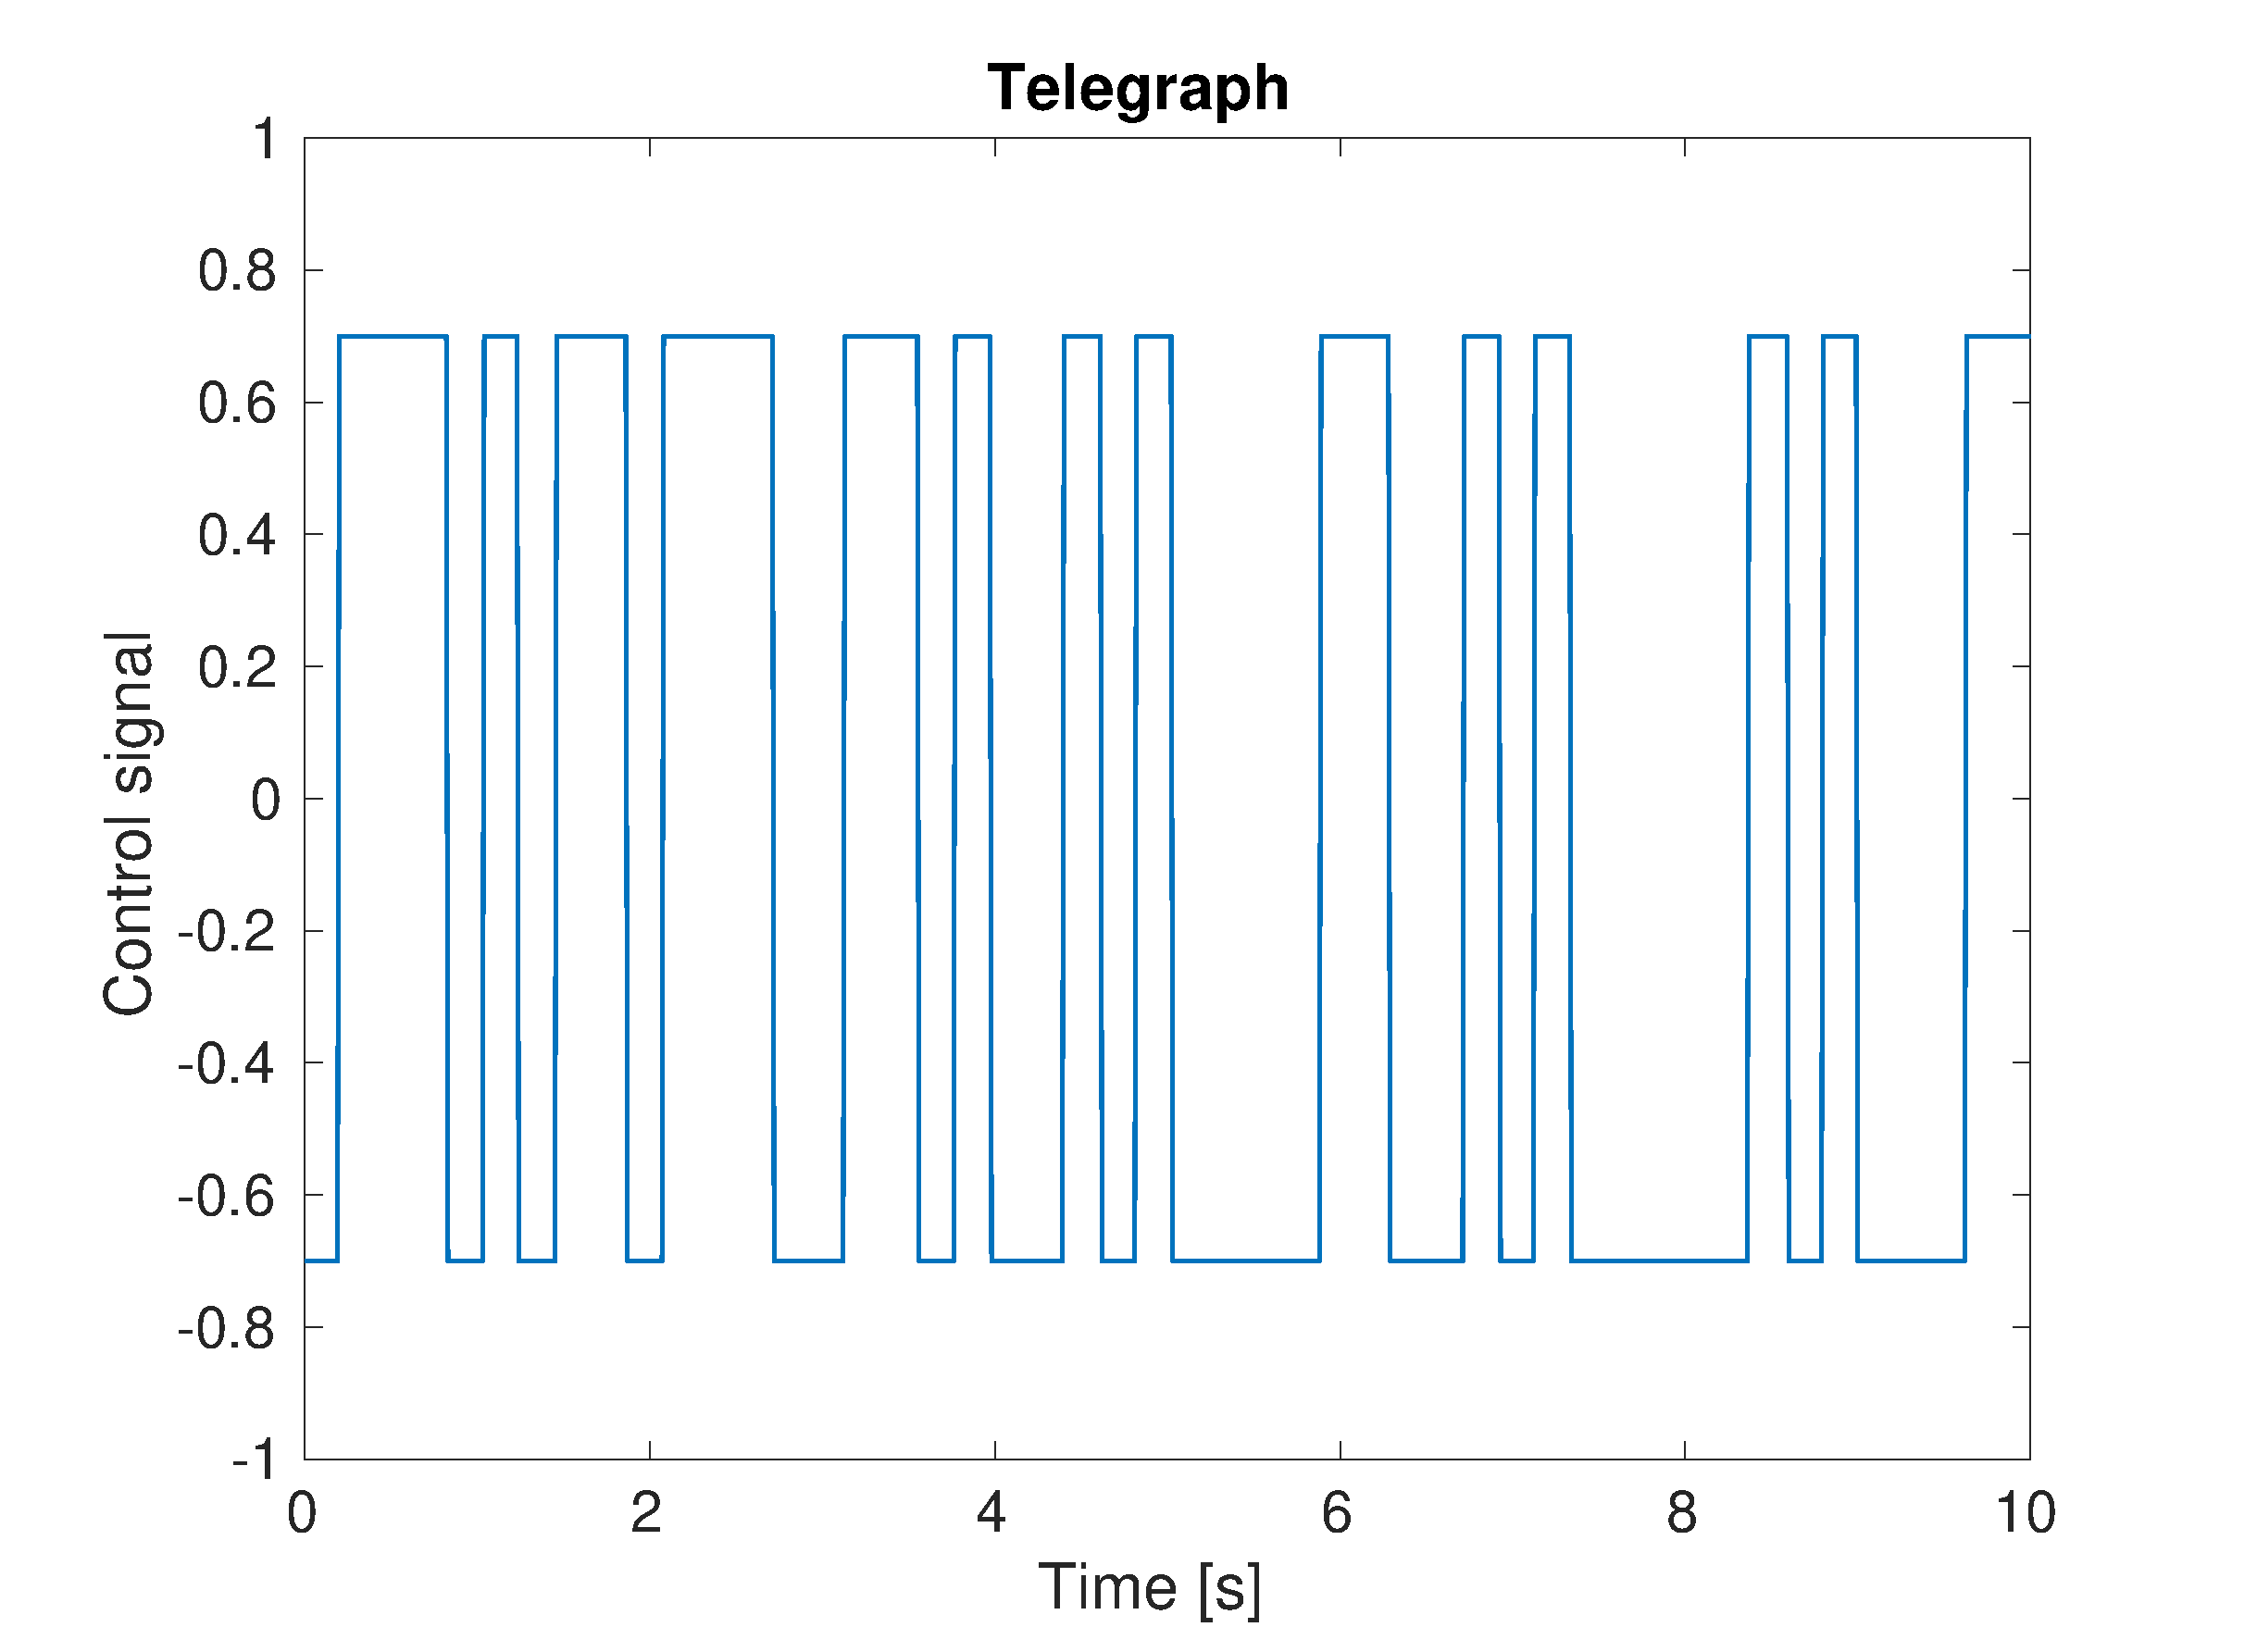
\includegraphics[width=0.8\textwidth]{telegraph}
\caption{An example of a telegraph signal which was sent to a thruster during data collection experiments.}
\label{fig:telegraph}
\end{figure}

Data preprocessing was done by synchronising the data streams by checking the start and end times of each experiment, here chosen as the time of arrival of the first control signal. The sensor data was aligned such that the data sample of each sensor whose arrival time was closest to the starting time of the test was chosen as the initial sample of each data stream. Data outside the test interval was discarded. After alignment the data was resampled to 100 Hz. The sensor data was resampled using first-order hold while the control signals were resampled using zero-order hold since the control signal data only contained points were the control signals changed.  

\begin{figure}[htbp]
  \centering
  \subfloat[][\label{fig:p_pqTest}Excitation in $p$ during $p$ and $q$ test.]{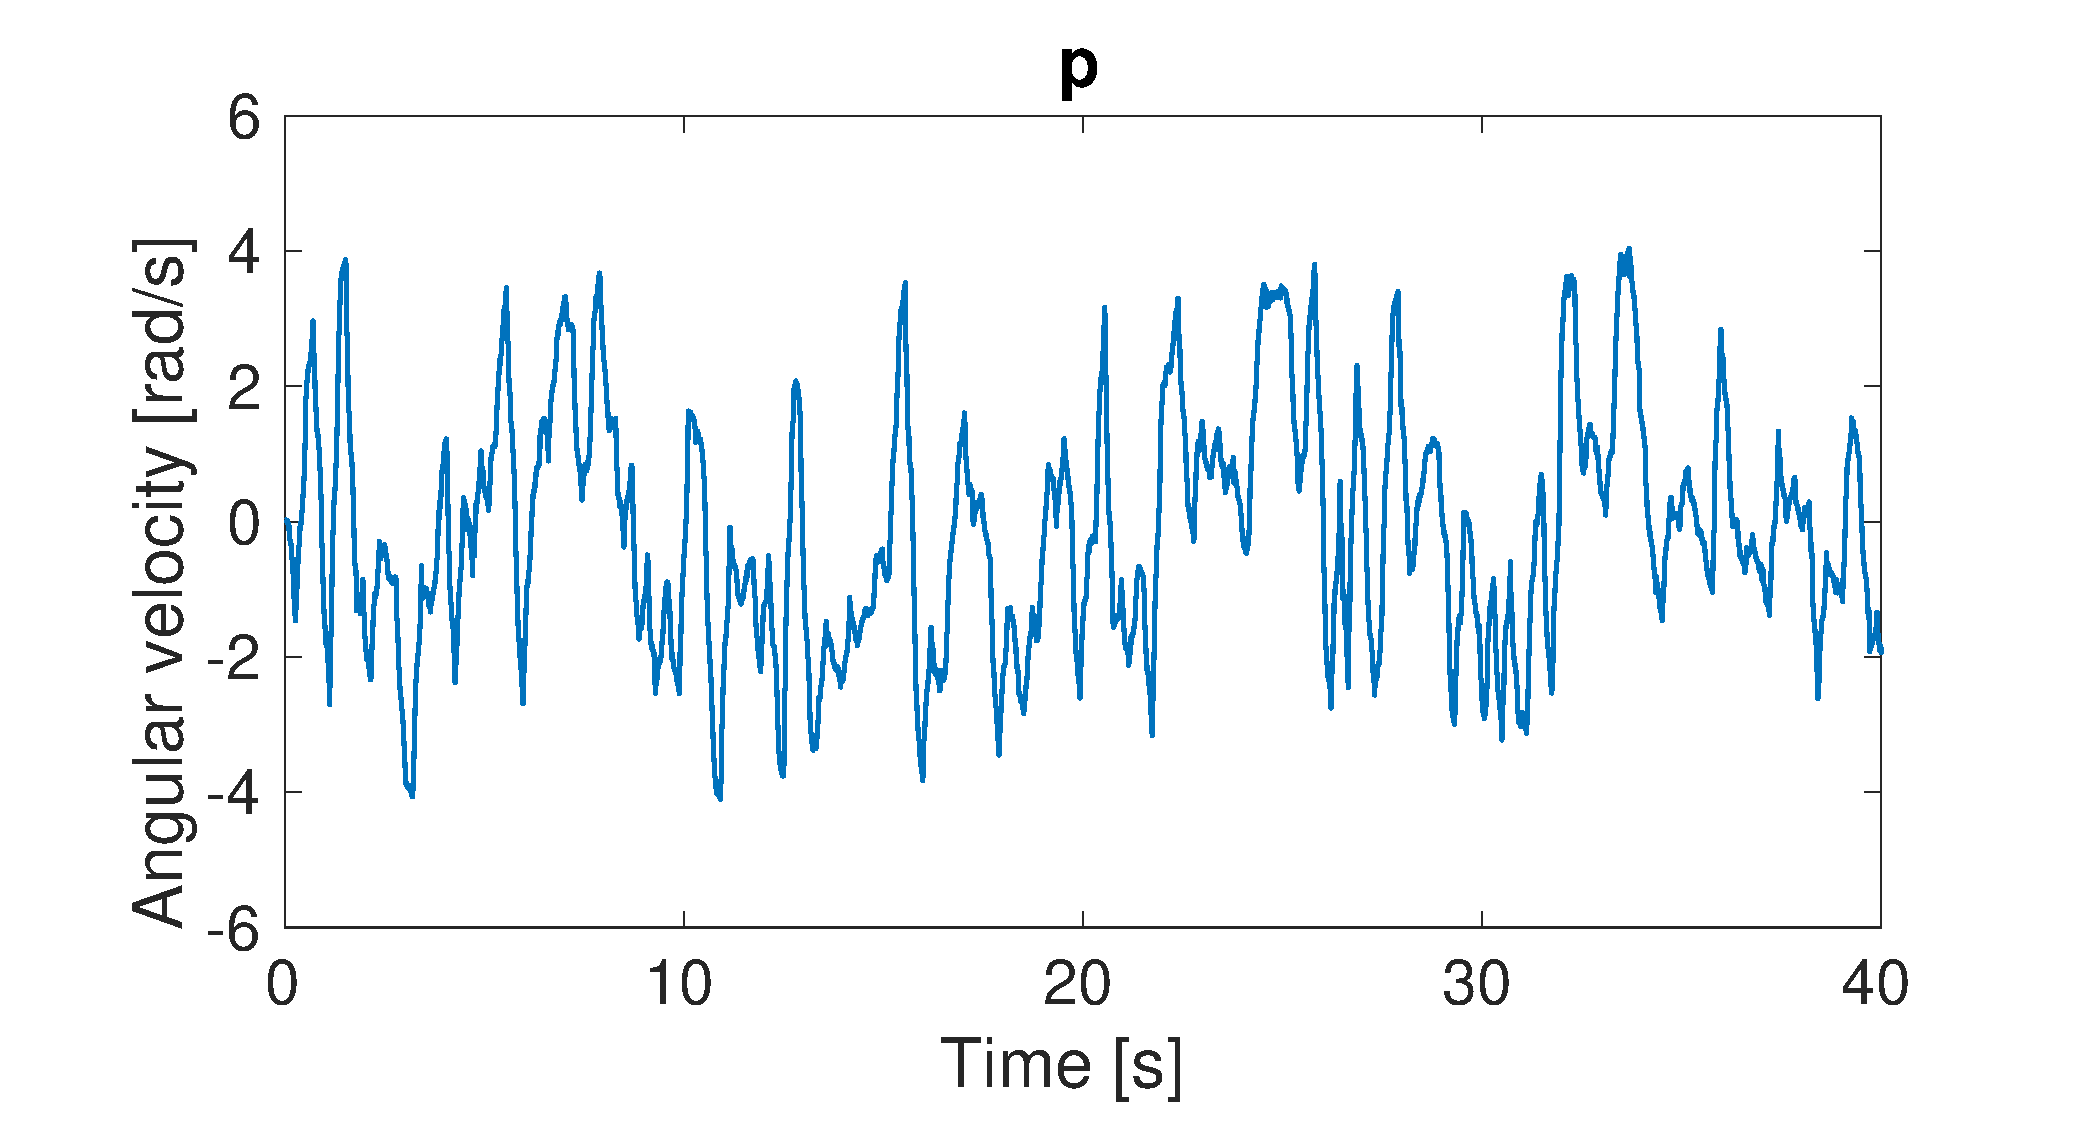
\includegraphics[width=0.4\textwidth]{p_pq_test}}
  \qquad
  \subfloat[][\label{fig:q_pqTest}Excitation in $q$ during $p$ and $q$ test.]{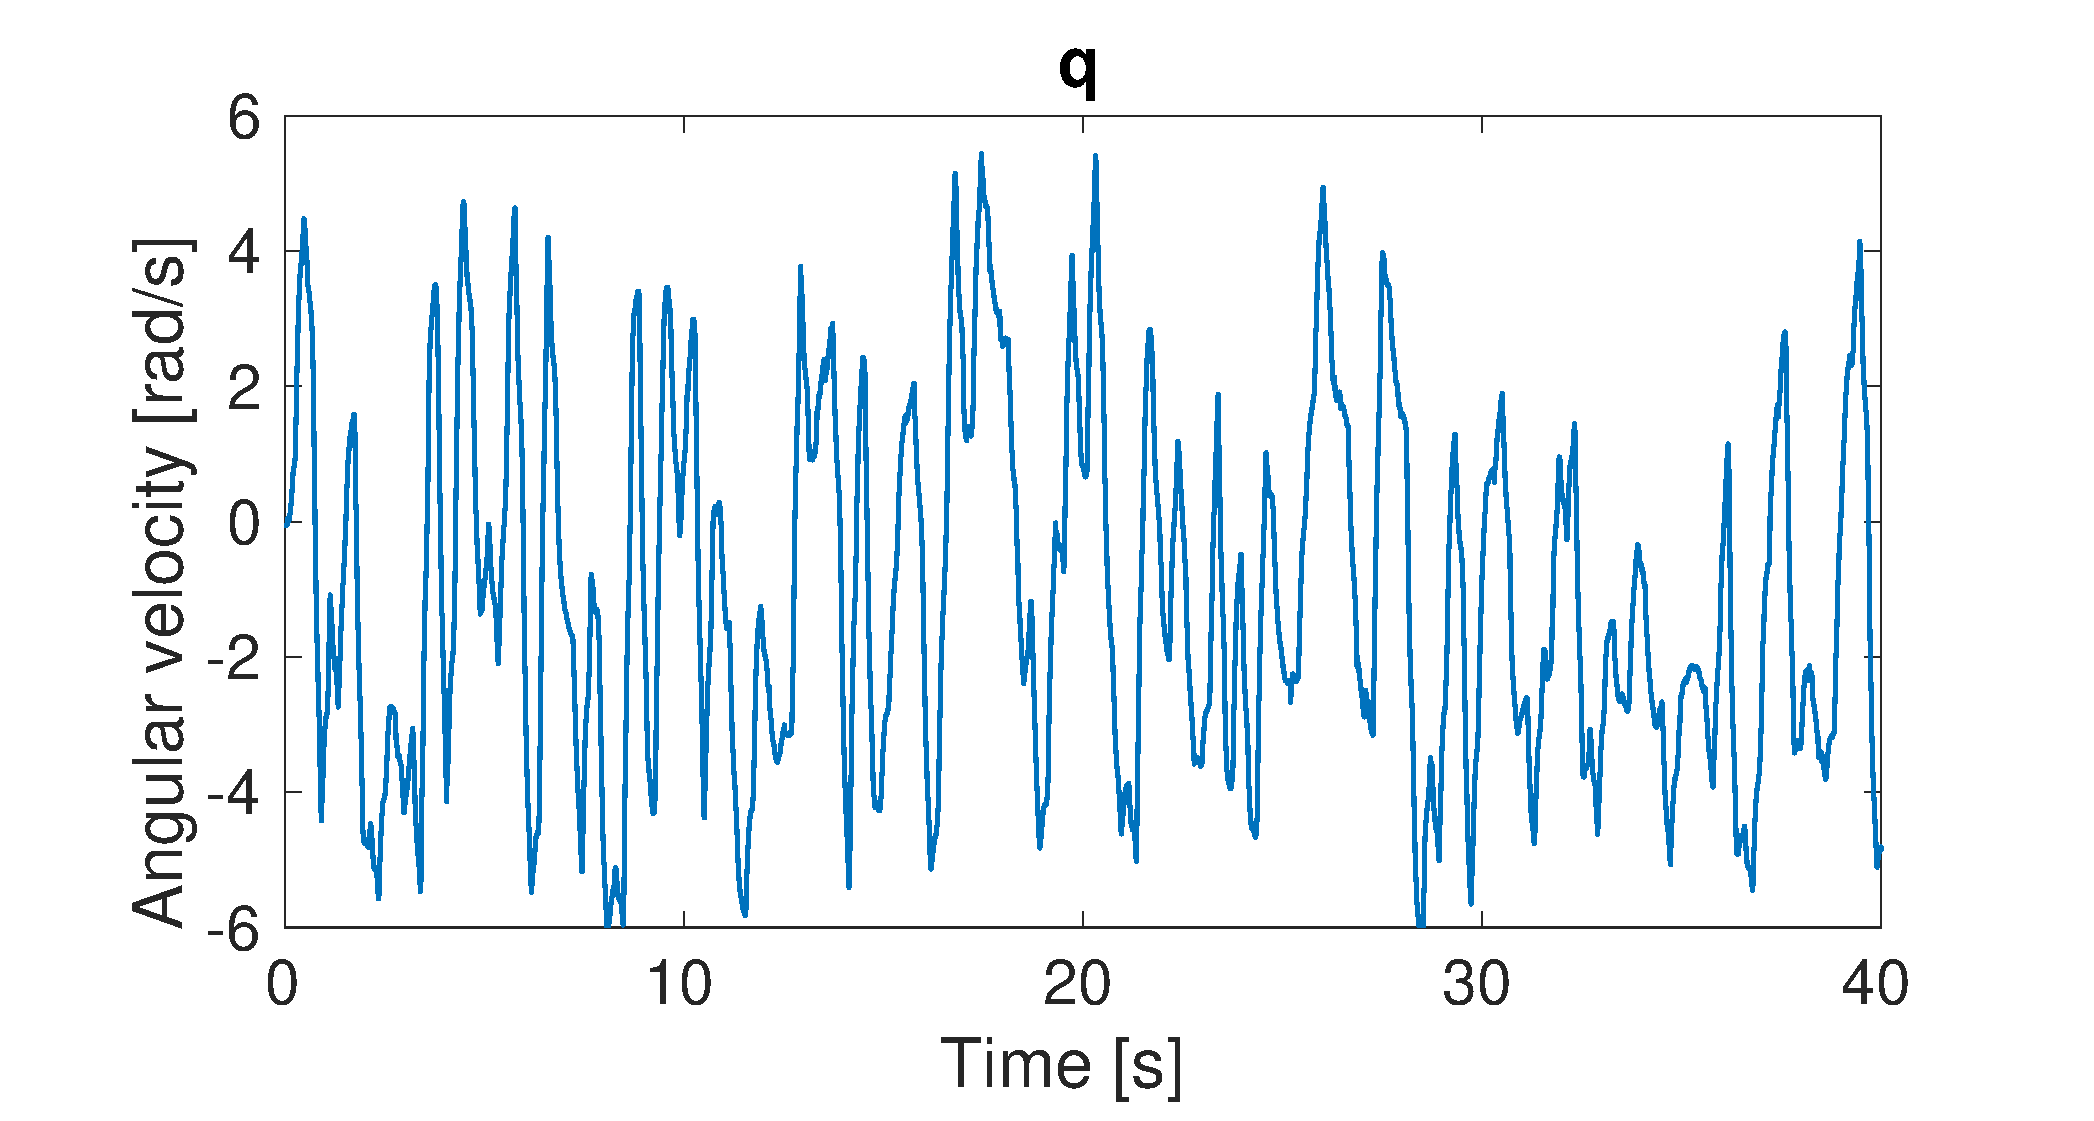
\includegraphics[width=0.4\textwidth]{q_pq_test}}
  \\
  \subfloat[][\label{fig:r_pqTest}Excitation in $r$ during $p$ and $q$ test.]{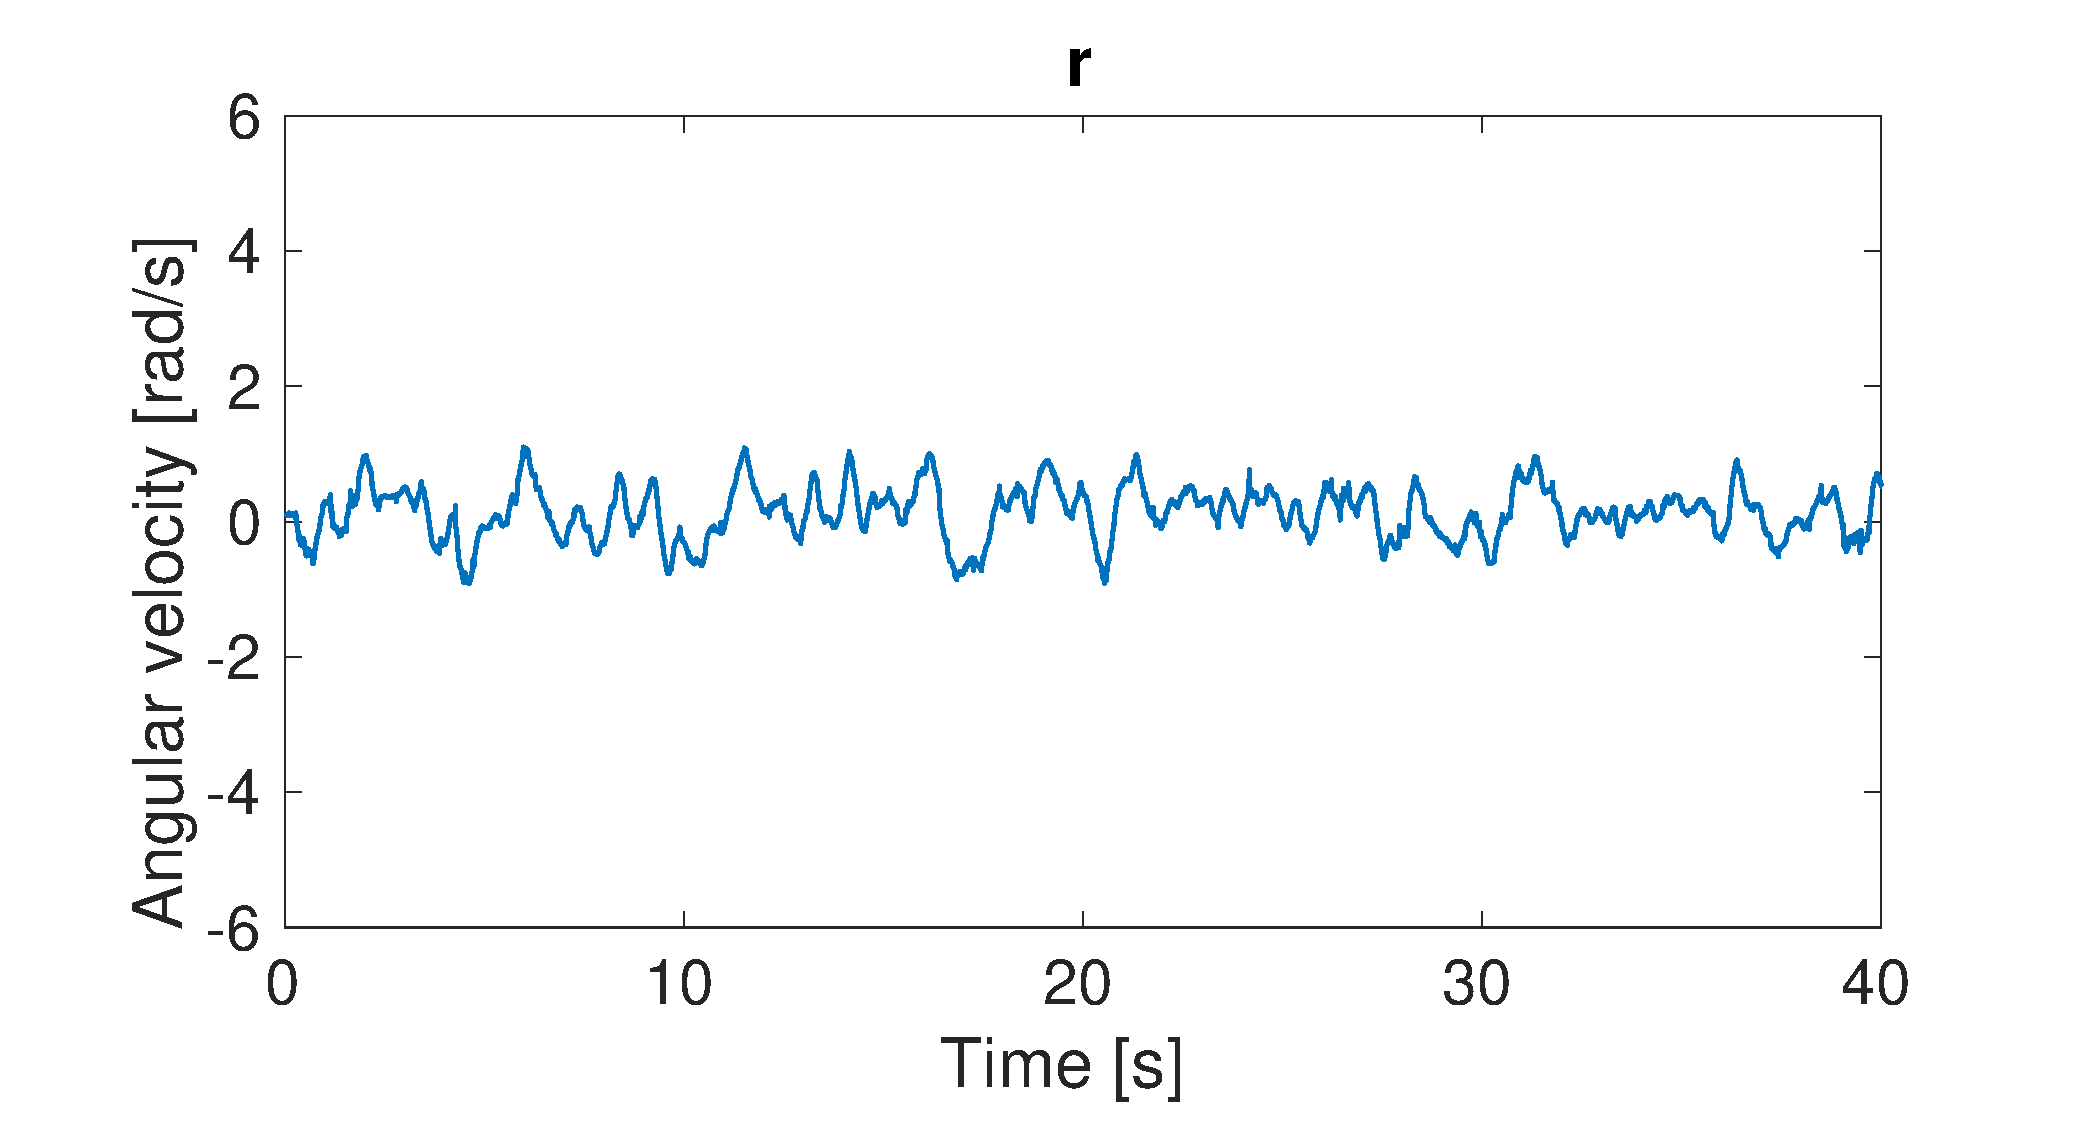
\includegraphics[width=0.4\textwidth]{r_pq_test}}
  \caption{\label{fig:pqTest}%
 Plots of excitation of the three angular velocities $p$, $q$ and $r$ from a test intended to mainly excite $p$ and $q$. Note that the amplitude in $r$ is four times smaller than that of $p$ and $q$.}
\end{figure}

\begin{figure}[htbp]
  \centering
  \subfloat[][\label{fig:p_rTest}Excitation in $p$ during $r$ test.]{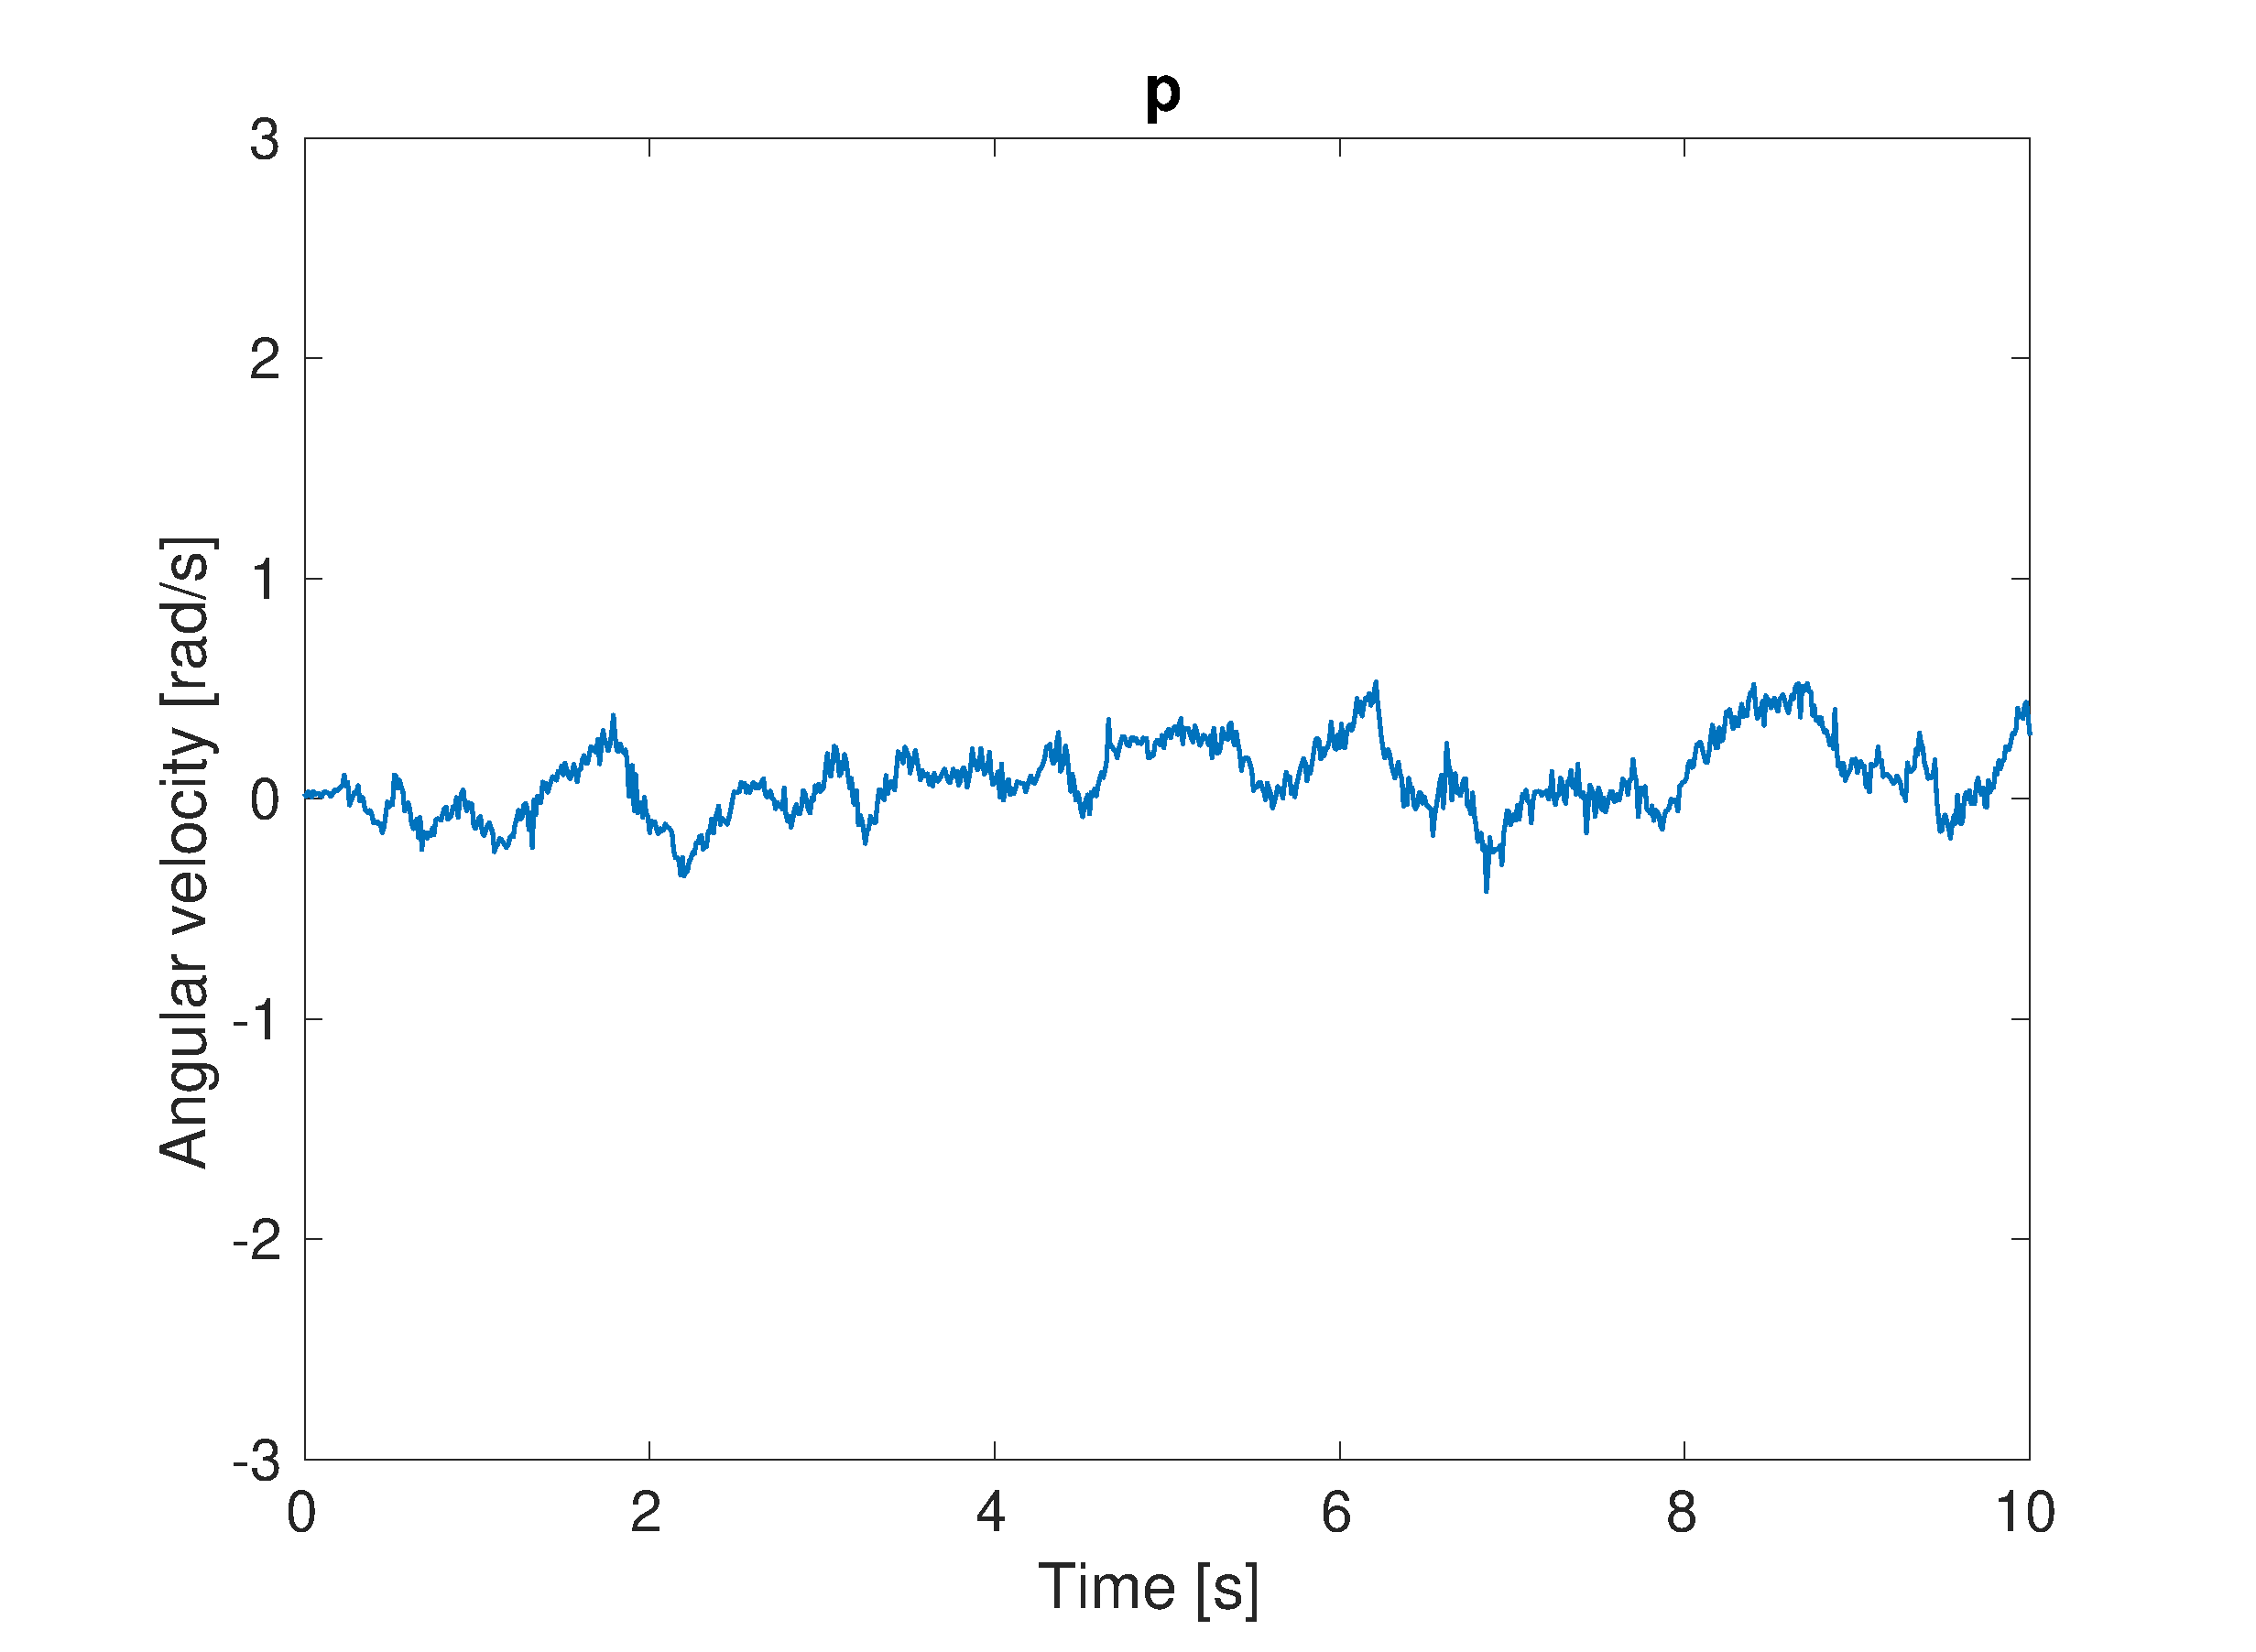
\includegraphics[width=0.4\textwidth]{p_r_test}}
  \qquad
  \subfloat[][\label{fig:q_rTest}Excitation in $q$ during $r$ test.]{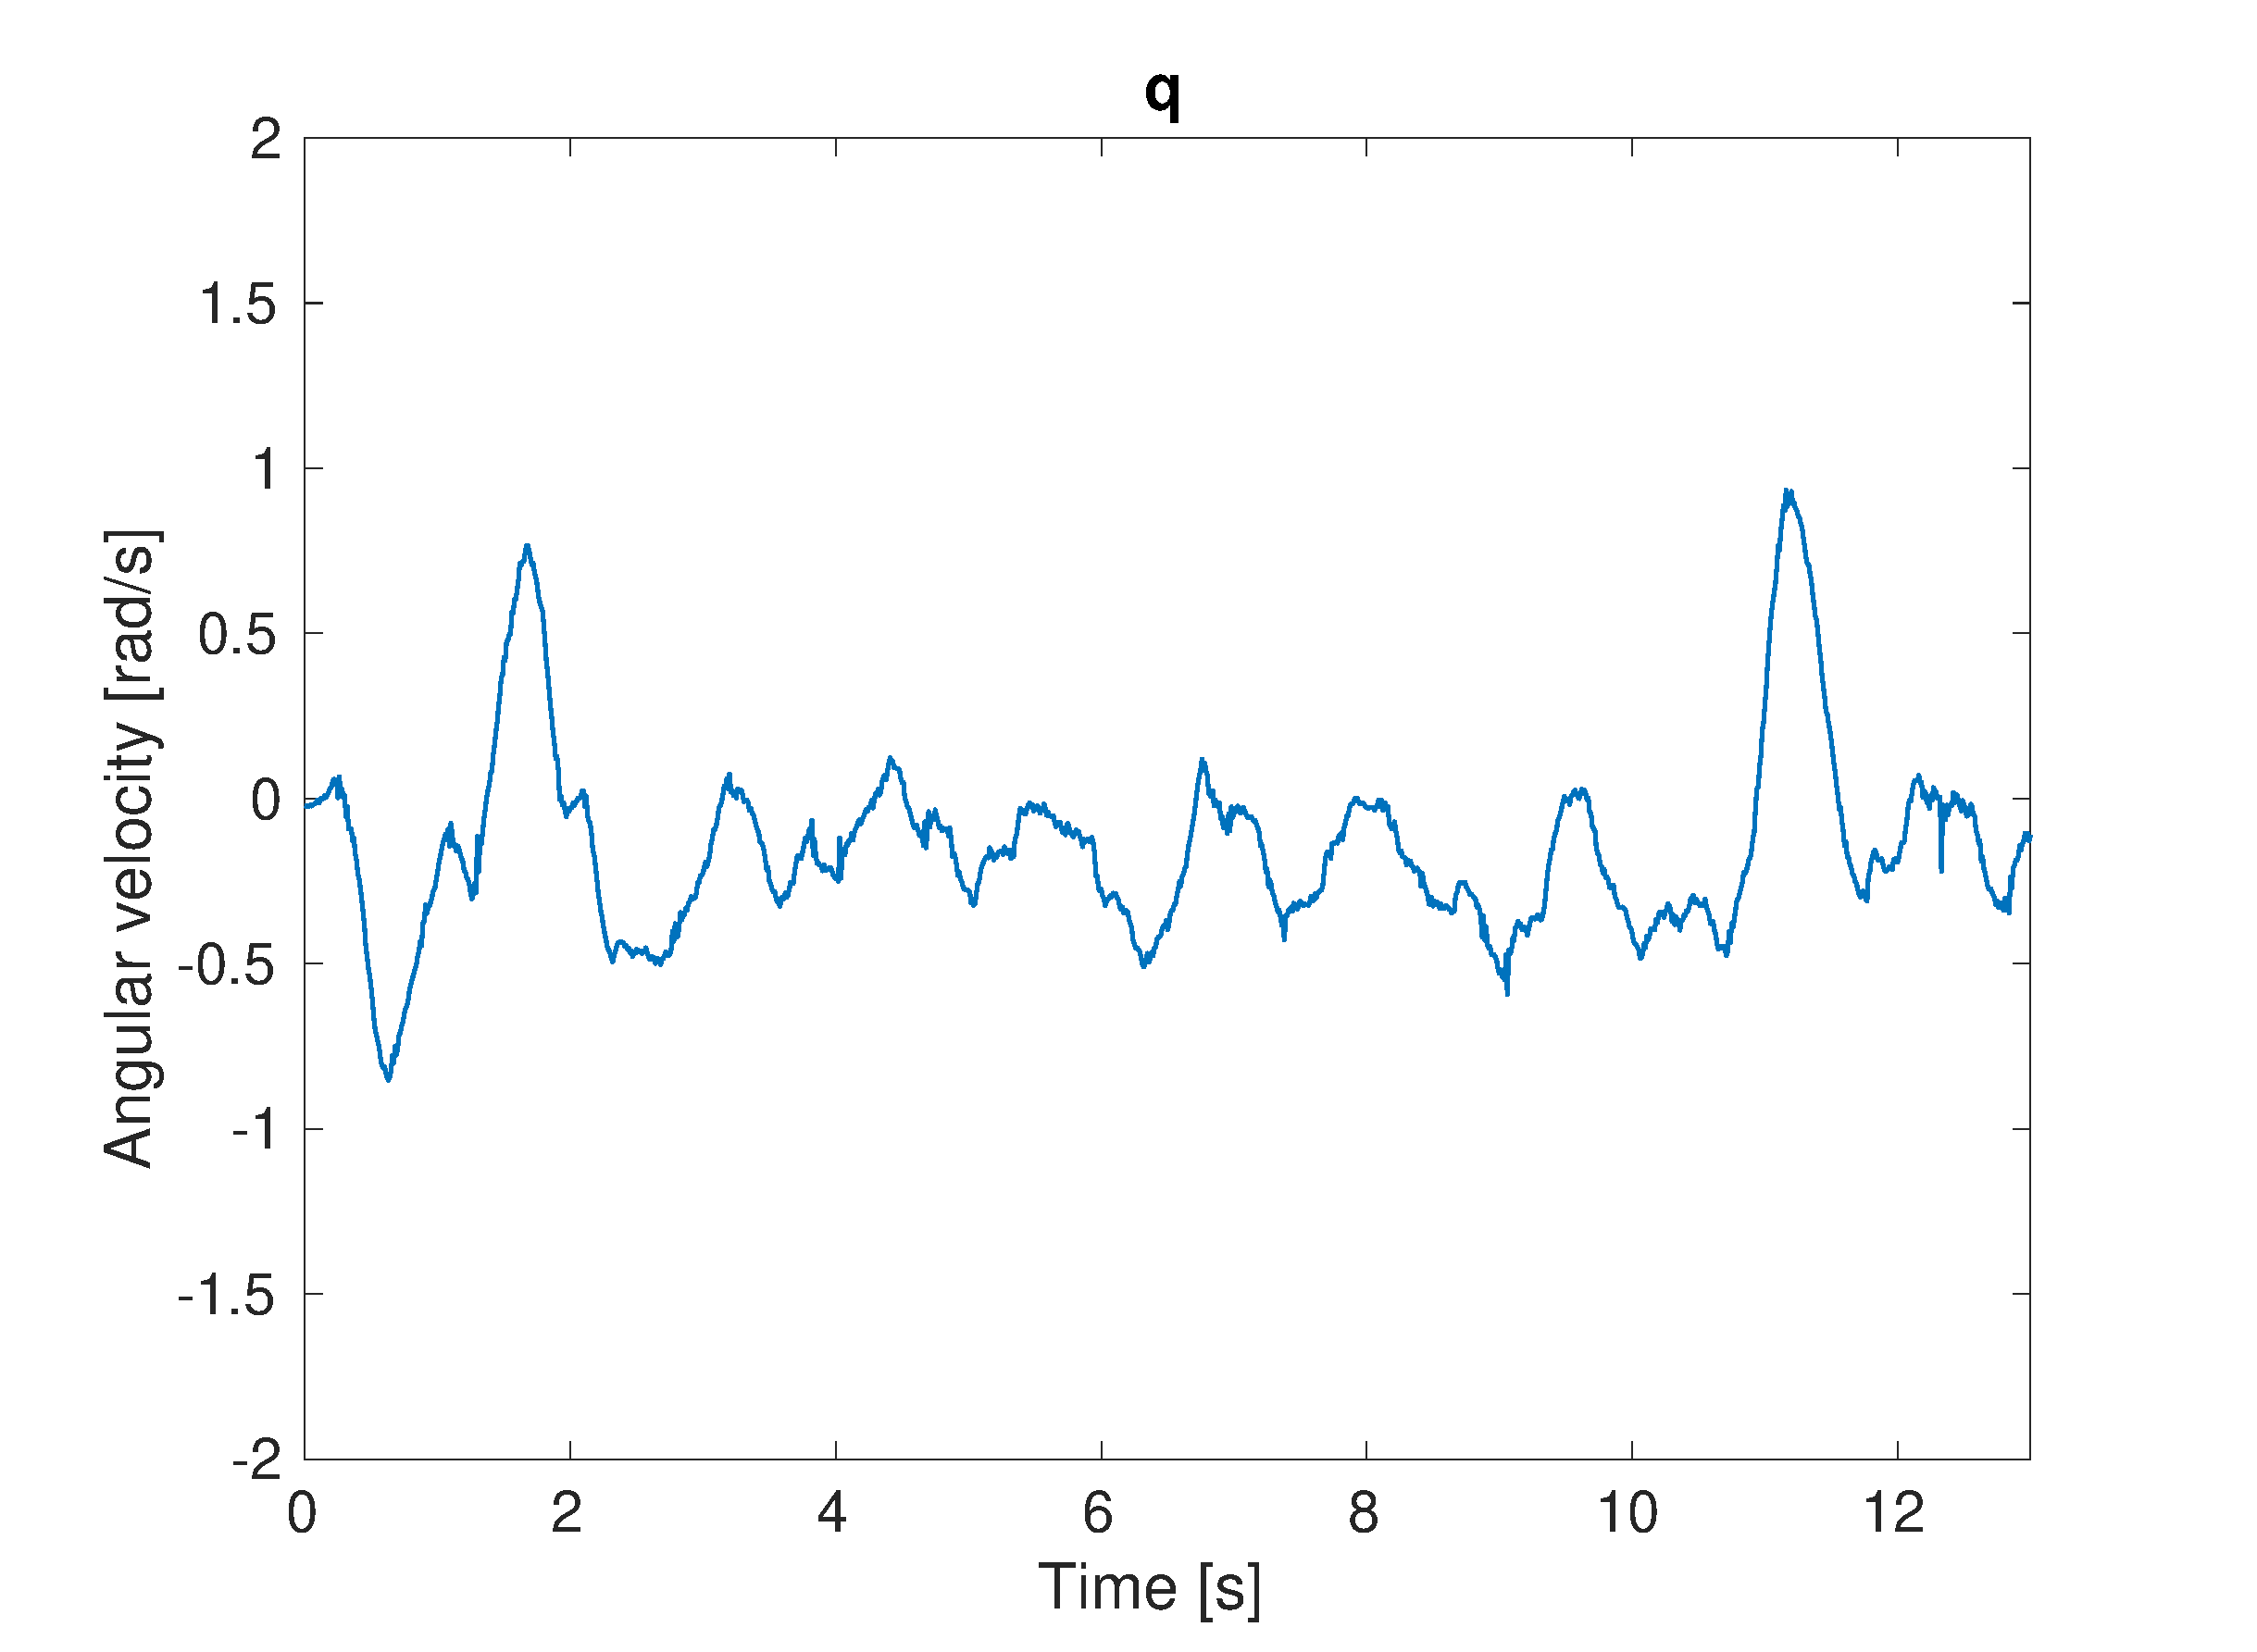
\includegraphics[width=0.4\textwidth]{q_r_test}}
  \\
  \subfloat[][\label{fig:r_rTest}Excitation in $r$ during $r$ test.]{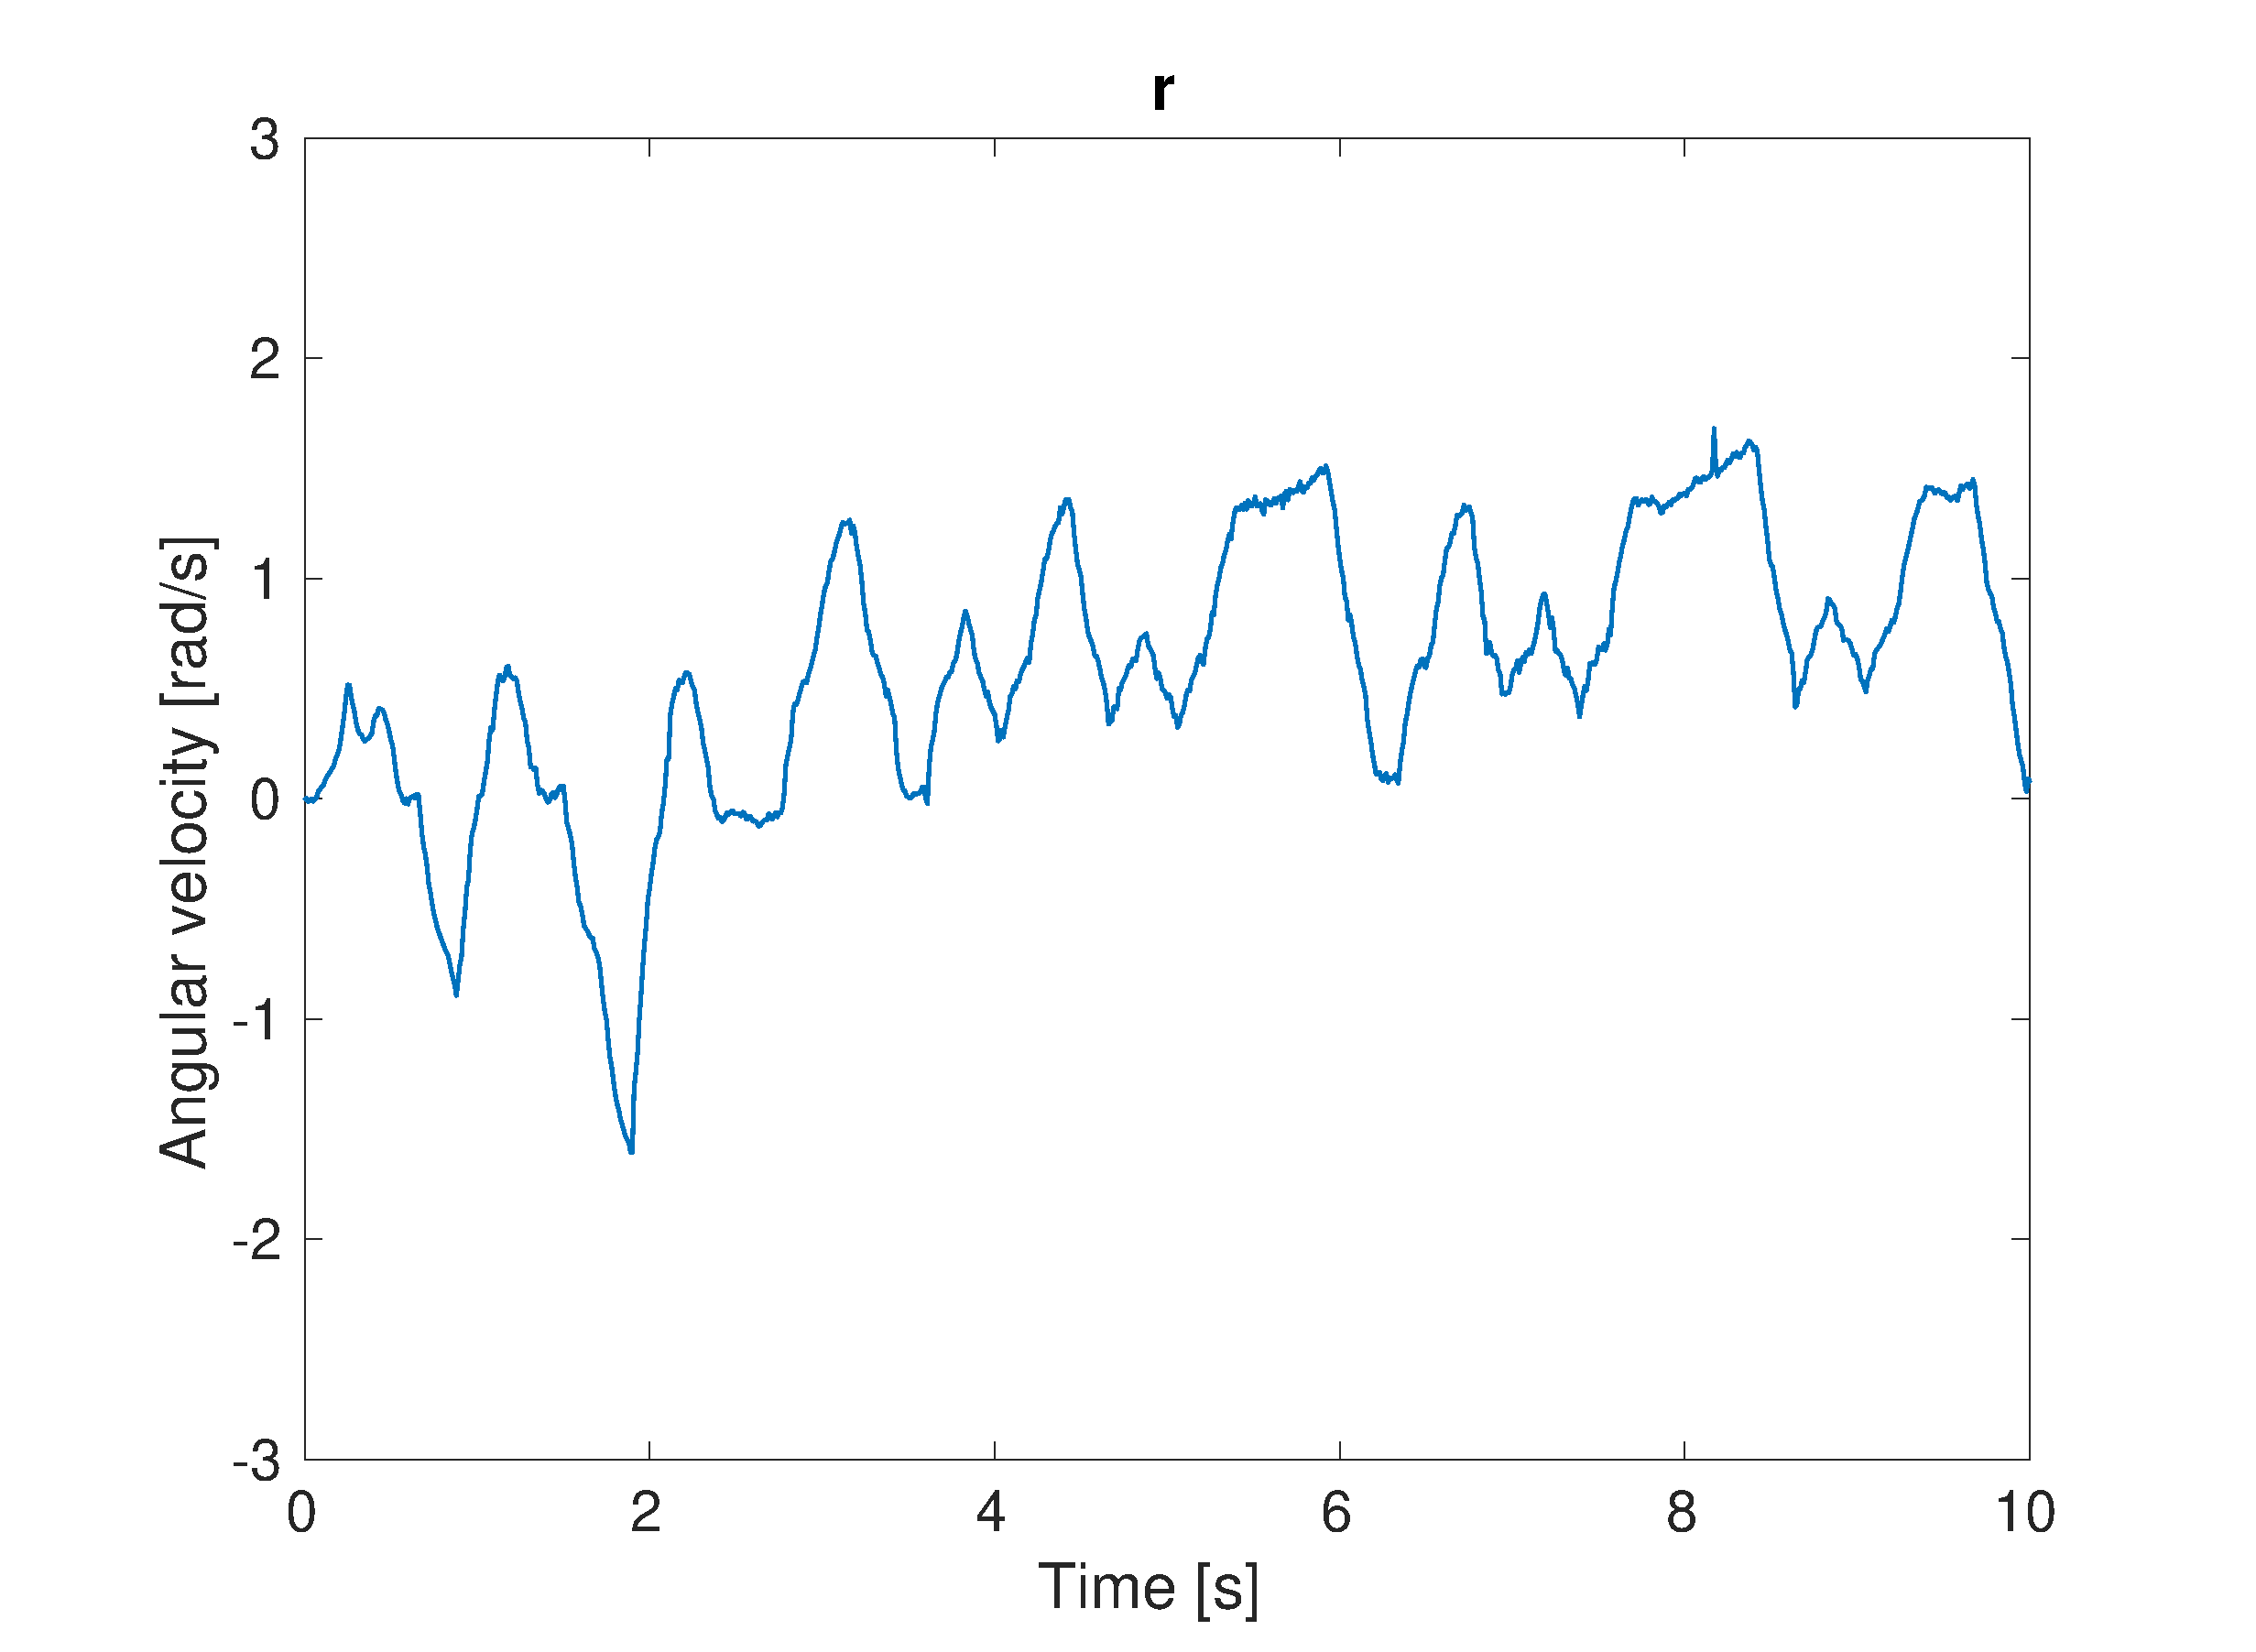
\includegraphics[width=0.4\textwidth]{r_r_test}}
  \caption{\label{fig:rTest}%
 Plots of excitation of the three angular velocities $p$, $q$ and $r$ from a test intended to mainly excite $r$. Note that the amplitude in $r$ is approximately two times larger than that of $p$ and $q$.}
\end{figure}
%%%%%%%%%%%%%%%%%%%%%%%%%%%%%%%%%
\section{Prediction-Error Method} \index{Cost function} \index{Prediction-Error Method}
The prediction-error method uses a predictor $\hat{\boldsymbol{y}}_k(\boldsymbol{\theta})$ of a model's output to compare with the present output of the system. The discrete-time predictor can be described by 
\begin{equation}
\hat{\boldsymbol{x}}_{k+1}(\theta) = f(\boldsymbol{\hat{x}_k}(\theta), \boldsymbol{u}_k,\boldsymbol{y}_k, \boldsymbol{\theta})
\end{equation}
and
\begin{equation}
\hat{\boldsymbol{y}}_k(\boldsymbol{\theta}) = h(\hat{\boldsymbol{x}}_k, \boldsymbol{u}_k, \boldsymbol{\theta})
\end{equation}
where $\hat{\boldsymbol{x}}$ is the estimated state vector, $\boldsymbol{u}$ are the inputs and $\hat{\boldsymbol{y}}_k(\boldsymbol{\theta})$ is the predicted output of the model \citep[p. 13]{Roger}. 

The fitting is done by minimising a cost function $V(\boldsymbol{\theta})$ with respect to the parameter vector $\boldsymbol{\theta}$ \emph{i.e.}
\begin{equation}
\hat{\boldsymbol{\theta}} = \underset{\boldsymbol{\theta}}{\argmin} V(\boldsymbol{\theta})
\end{equation}
The cost function in this thesis has been defined as the squared error with an error threshold to handle noisy signals. An error threshold means that after a breakpoint the cost function becomes linear instead of quadratic, which makes the parameter estimation less sensitive to outliers. To reduce the impact of the noise even further, the weight matrix was chosen as the inverse of the estimated noise covariance \citep{ljungtheory}. The cost function is then
\begin{equation}
    V(\boldsymbol{\theta}) = \frac{1}{N} \left( \sum_{t \in i} \boldsymbol{e}^T_k(\boldsymbol{\theta}) \boldsymbol{W}(\boldsymbol{\theta})  \boldsymbol{e}_k(\boldsymbol{\theta}) + \sum_{t \in j} \boldsymbol{v}^T_k(\boldsymbol{\theta}) \boldsymbol{W}(\boldsymbol{\theta})  \boldsymbol{v}_k(\boldsymbol{\theta}) \right)
\end{equation}
where $N$ is the number of samples in the dataset, $\boldsymbol{e}_k(\boldsymbol{\theta})$ is the error vector with the parameter vector~$\boldsymbol{\theta}$ and $\boldsymbol{W}$ is a positive definite weight matrix \citep{ljungtheory}. The set $i$ is the subset of errors for which $\abs{\boldsymbol{e}_k(\boldsymbol{\theta})} < \sigma \rho$ holds. Here, $\sigma$ is the estimated standard deviation of $\boldsymbol{e}_k(\boldsymbol{\theta})$ and $\rho$ is the chosen error threshold. The set $j$ is the complement of $i$. The error $\boldsymbol{v}_k(\boldsymbol{\theta})$ is defined as 
\begin{equation}
\boldsymbol{v}_k(\boldsymbol{\theta}) = \boldsymbol{e}_k(\boldsymbol{\theta}) \sigma\frac{\rho}{\sqrt{\abs{\boldsymbol{e}_k(\boldsymbol{\theta})}}}
\end{equation}

%Several tools exists	which can estimate parameters using the prediction-error method. In this thesis the System Identification Toolbox\texttrademark has been used.
%%%%%%%%%%%%%%%%%%%%%%%%%%%%%%%%%%%%%%%%%%%%%%%%%%%%%%%%%%%
\section{Estimation Using Prediction-Error Method} \label{sec:pem} \index{Fit} \index{Model structure}
A initial set of model parameters were estimated using \eqref{eq:pq_dot_decouple} and \eqref{eq:r_dot_decouple}, while using appropriate data sets. These initial parameters were then used in model \eqref{eq:quatModel}. Estimated angles were used as inputs and angular velocities as outputs. This gave the following model structure to be estimated
\begin{equation}
\dot{\hat{\boldsymbol{\eta}}} = f(\hat{\nuVector}, \bar{\etaVector}, \tauVector)
\end{equation}
and
\begin{equation}
\hat{\boldsymbol{y}} = \hat{\nuVector}
\end{equation}
where $\bar{\etaVector} = \hat{\etaVector}$ are the estimated Euler angles from the sensor fusion.
The result of the estimation can be seen in \Tableref{tab:ResultEstimAngular}.  The fit of the model compared to validation data can be seen in \Figureref{fig:velocityCompareCong}. The model has a high fit of $50-60\ \%$ and thus describes the validation data well.
%The estimation used two datasets as estimation data and used one dataset for validation data.%
\begin{figure}[tbp]
  \centering
  \subfloat[][\label{fig:velocityCompareCongp}Simulated model and validation data in $p$.]{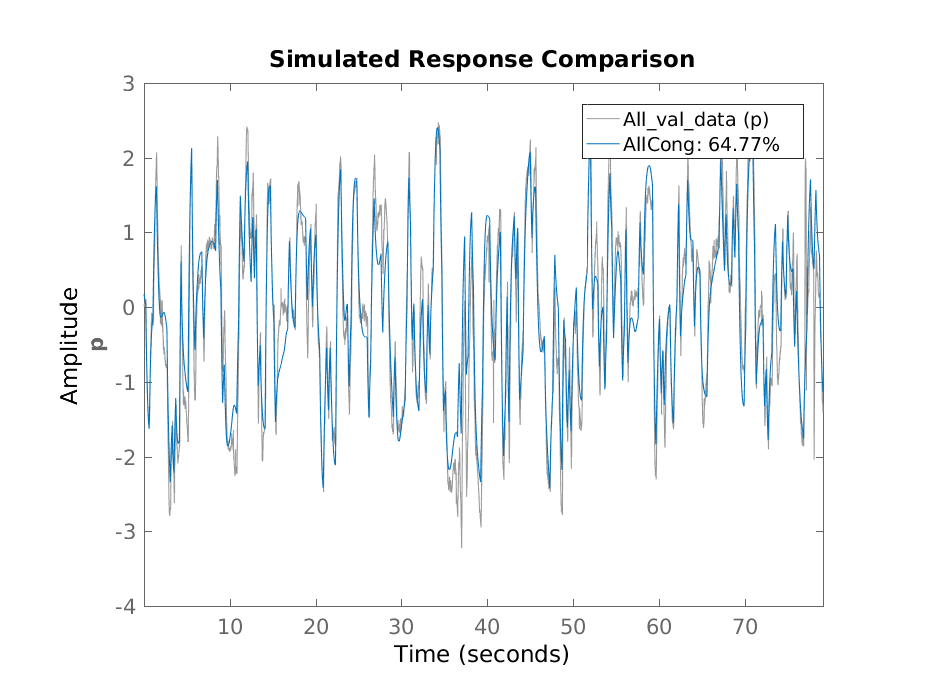
\includegraphics[width=0.4\textwidth]{velocityCompareCongp}}
  \qquad
  \subfloat[][\label{fig:velocityCompareCongq}Simulated model and validation data in $q$.]{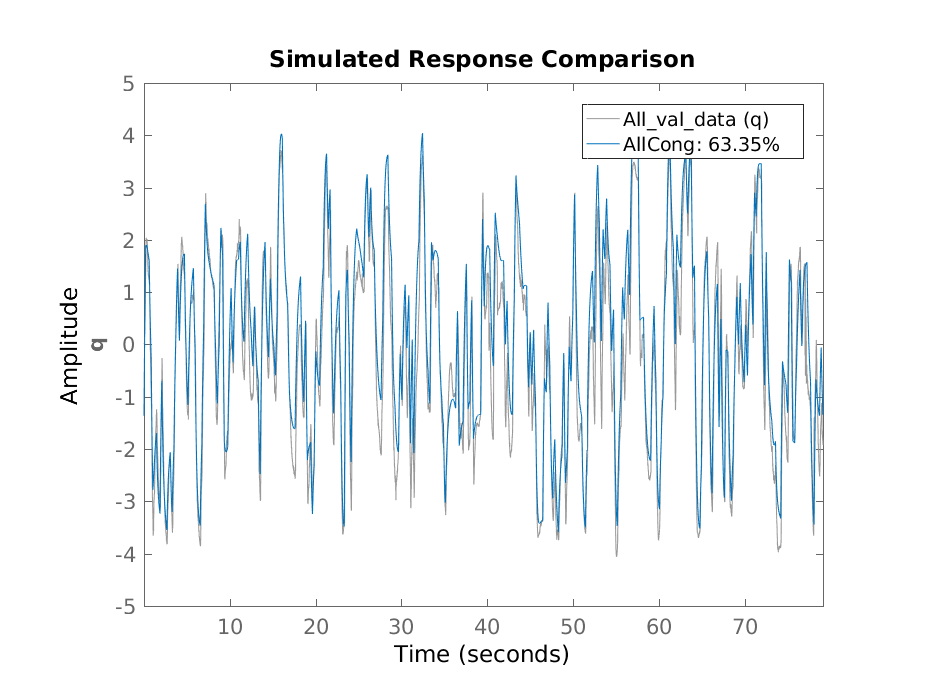
\includegraphics[width=0.4\textwidth]{velocityCompareCongq}}
  \\
  \subfloat[][\label{fig:velocityCompareCongr}Simulated model and validation data in $r$.]{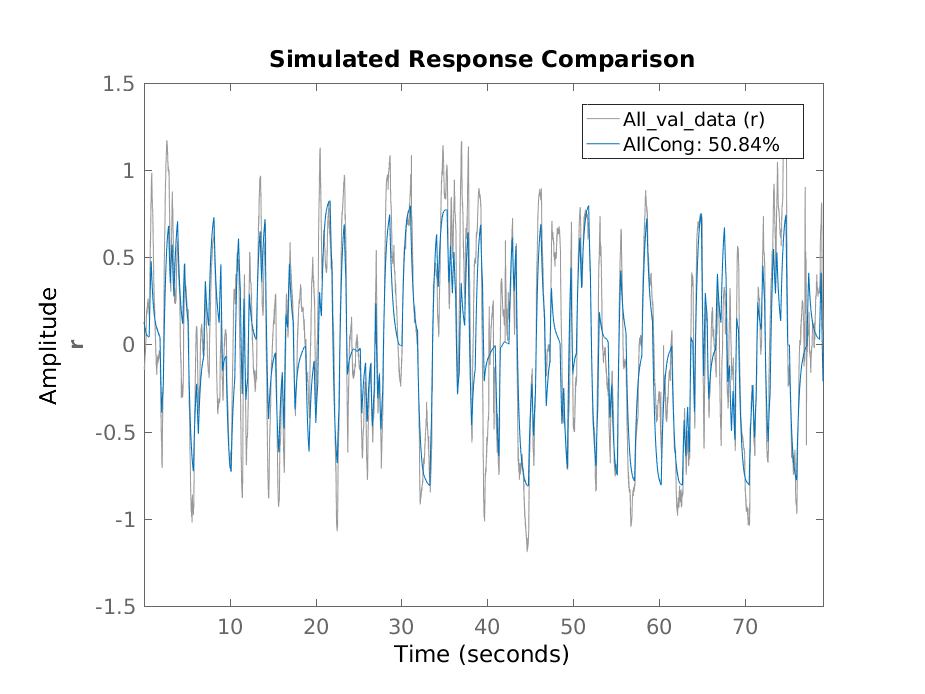
\includegraphics[width=0.4\textwidth]{velocityCompareCongr}}
  \caption{\label{fig:velocityCompareCong}%
    Comparison of simulation of the attitude model (blue) against validation data (gray) using the estimated angels as inputs and angular velocities as outputs. The simulated model has a high fit compared to the validation data.}
\end{figure}

The estimate of $\etaVector$ did not follow the kinematic relations described in \sectionref{sec:coordinates}. The problem with $\etaVector$ not following the kinematic relations was further investigated by comparing integration of \eqref{eq:eulerAnglesdot} with $\hat{\etaVector}$ from the sensor fusion. As can be seen in \Figureref{fig:integratedAngleVelocities} the result was not satisfactory, with the estimated angles and the integration of \eqref{eq:eulerAnglesdot} being very dissimilar. It was therefore concluded that the estimated angles were unfit for use as outputs during parameter estimation unless a new motion model for the sensor fusion was created to solve the issue. It is therefore recommended that the validity of the observer is controlled using relations such as those in \sectionref{sec:coordinates} before collecting data. 

\begin{figure}[htbp]
  \centering
  \subfloat[][\label{fig:velocityAnglePhi}Comparison between integration of $\dot{\phi}$ and $\hat{\phi}$ from the \abbrEKF]{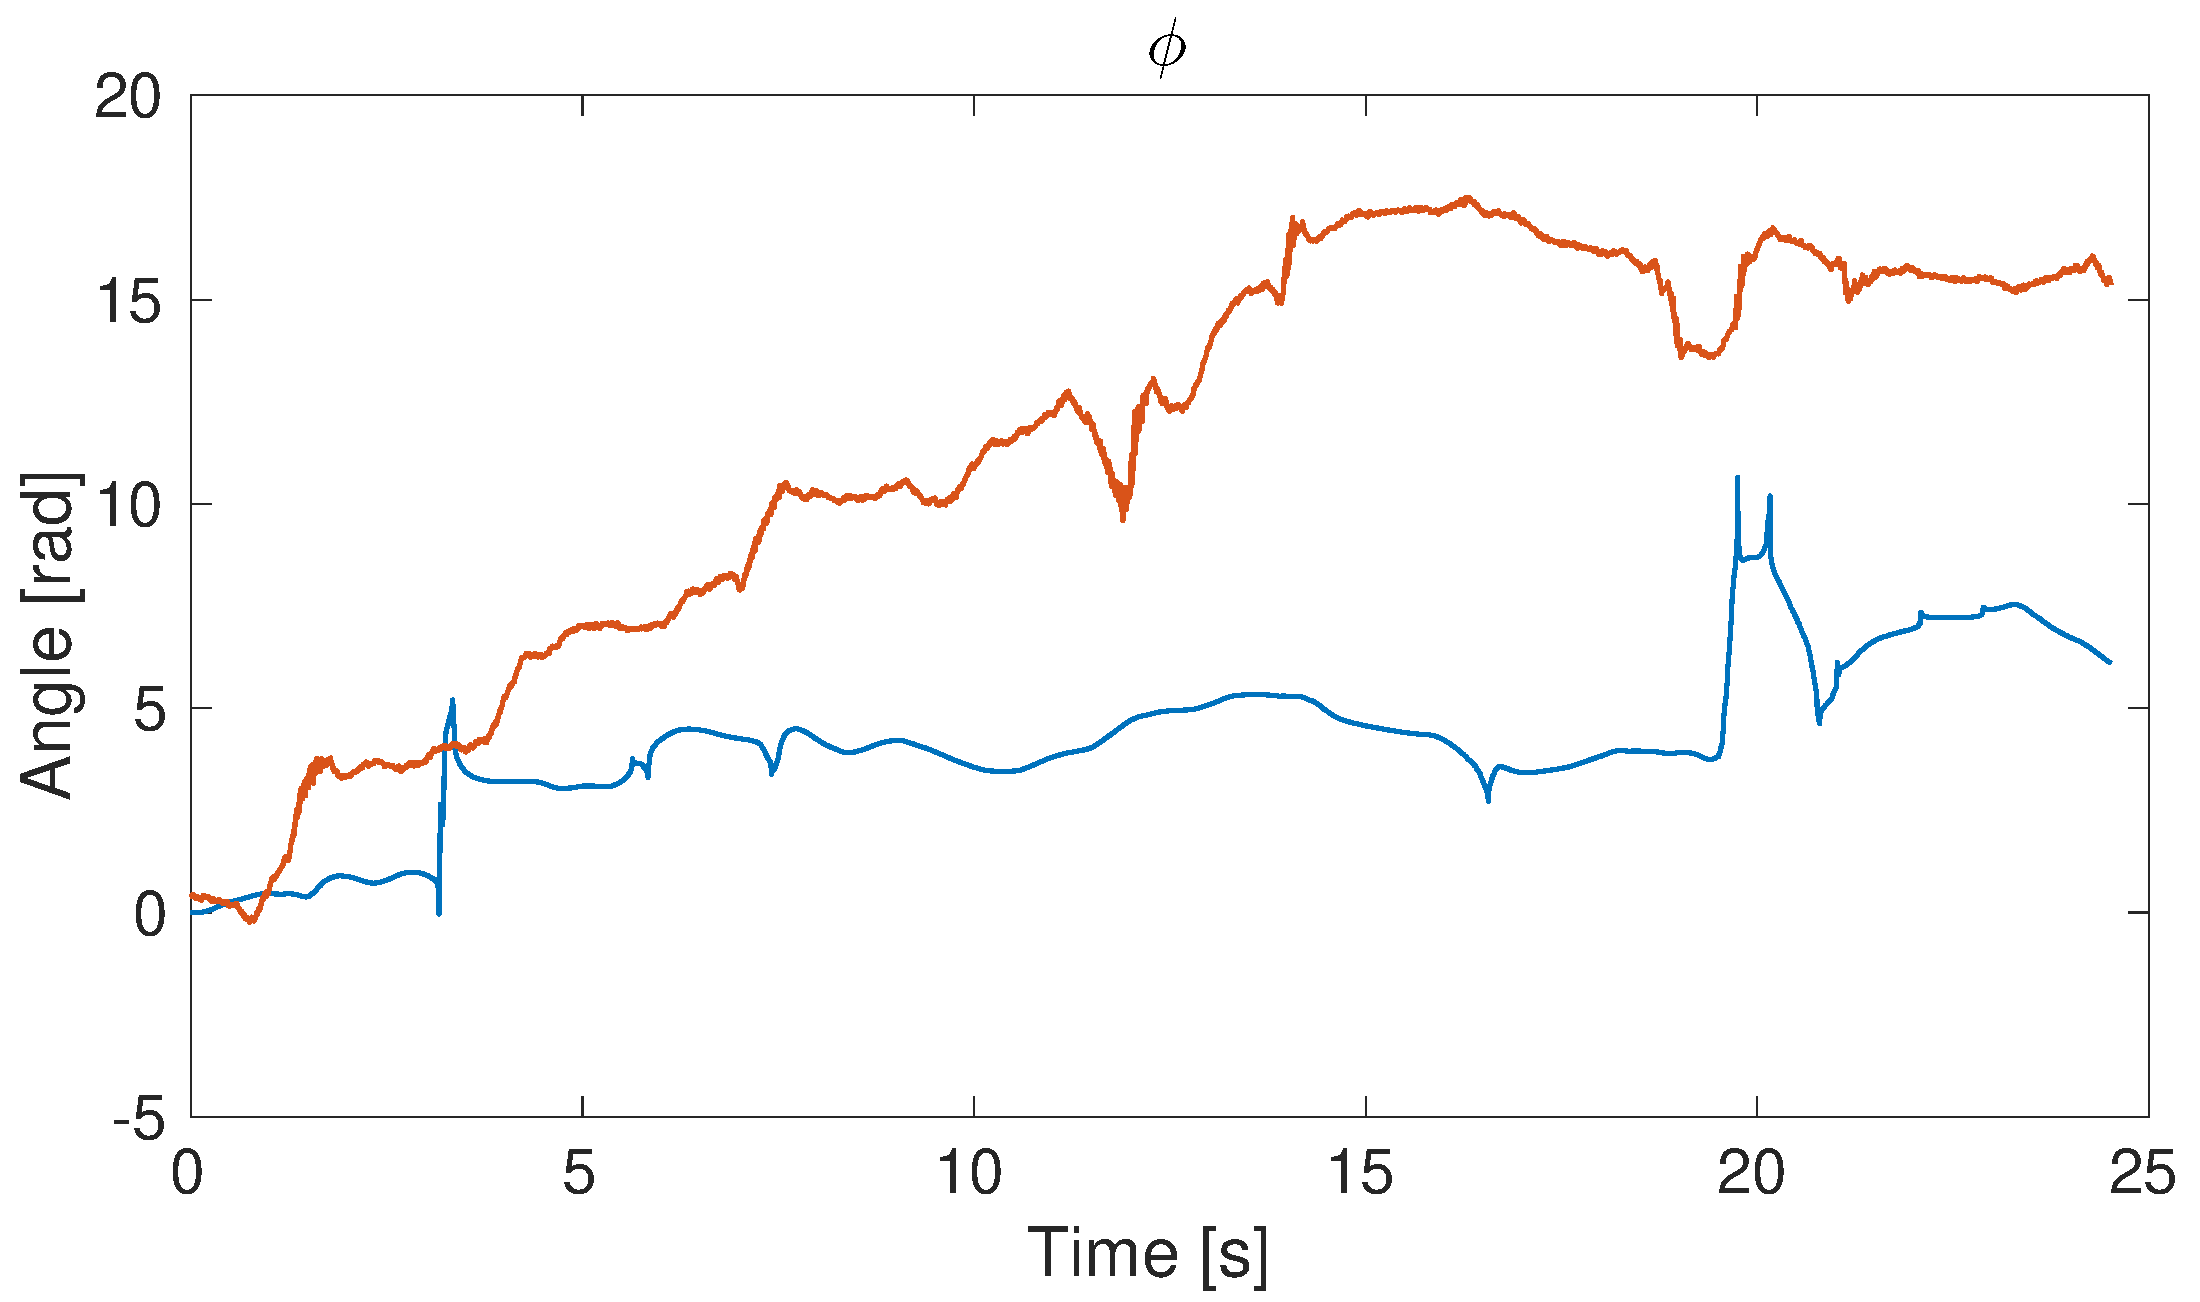
\includegraphics[width=0.4\textwidth]{velocityAnglePhi}}
  \qquad
  \subfloat[][\label{fig:velocityAngleTheta}Comparison between integration of $\dot{\theta}$ and $\hat{\theta}$ from the \abbrEKF]{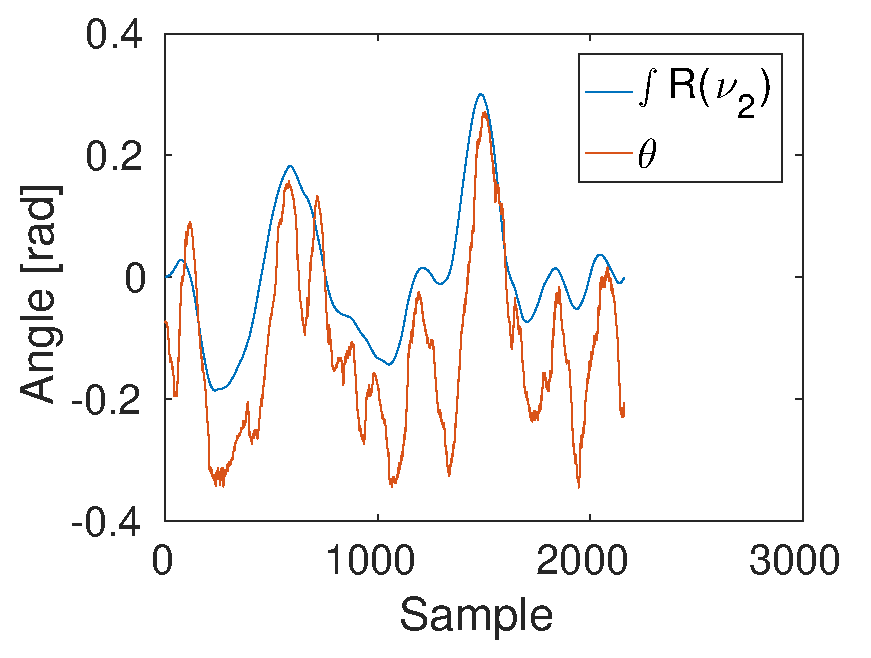
\includegraphics[width=0.4\textwidth]{velocityAngleTheta}}
  \\
  \subfloat[][\label{fig:velocityAnglePsi}Comparison between integration of $\dot{\psi}$ and $\hat{\psi}$ from the \abbrEKF]{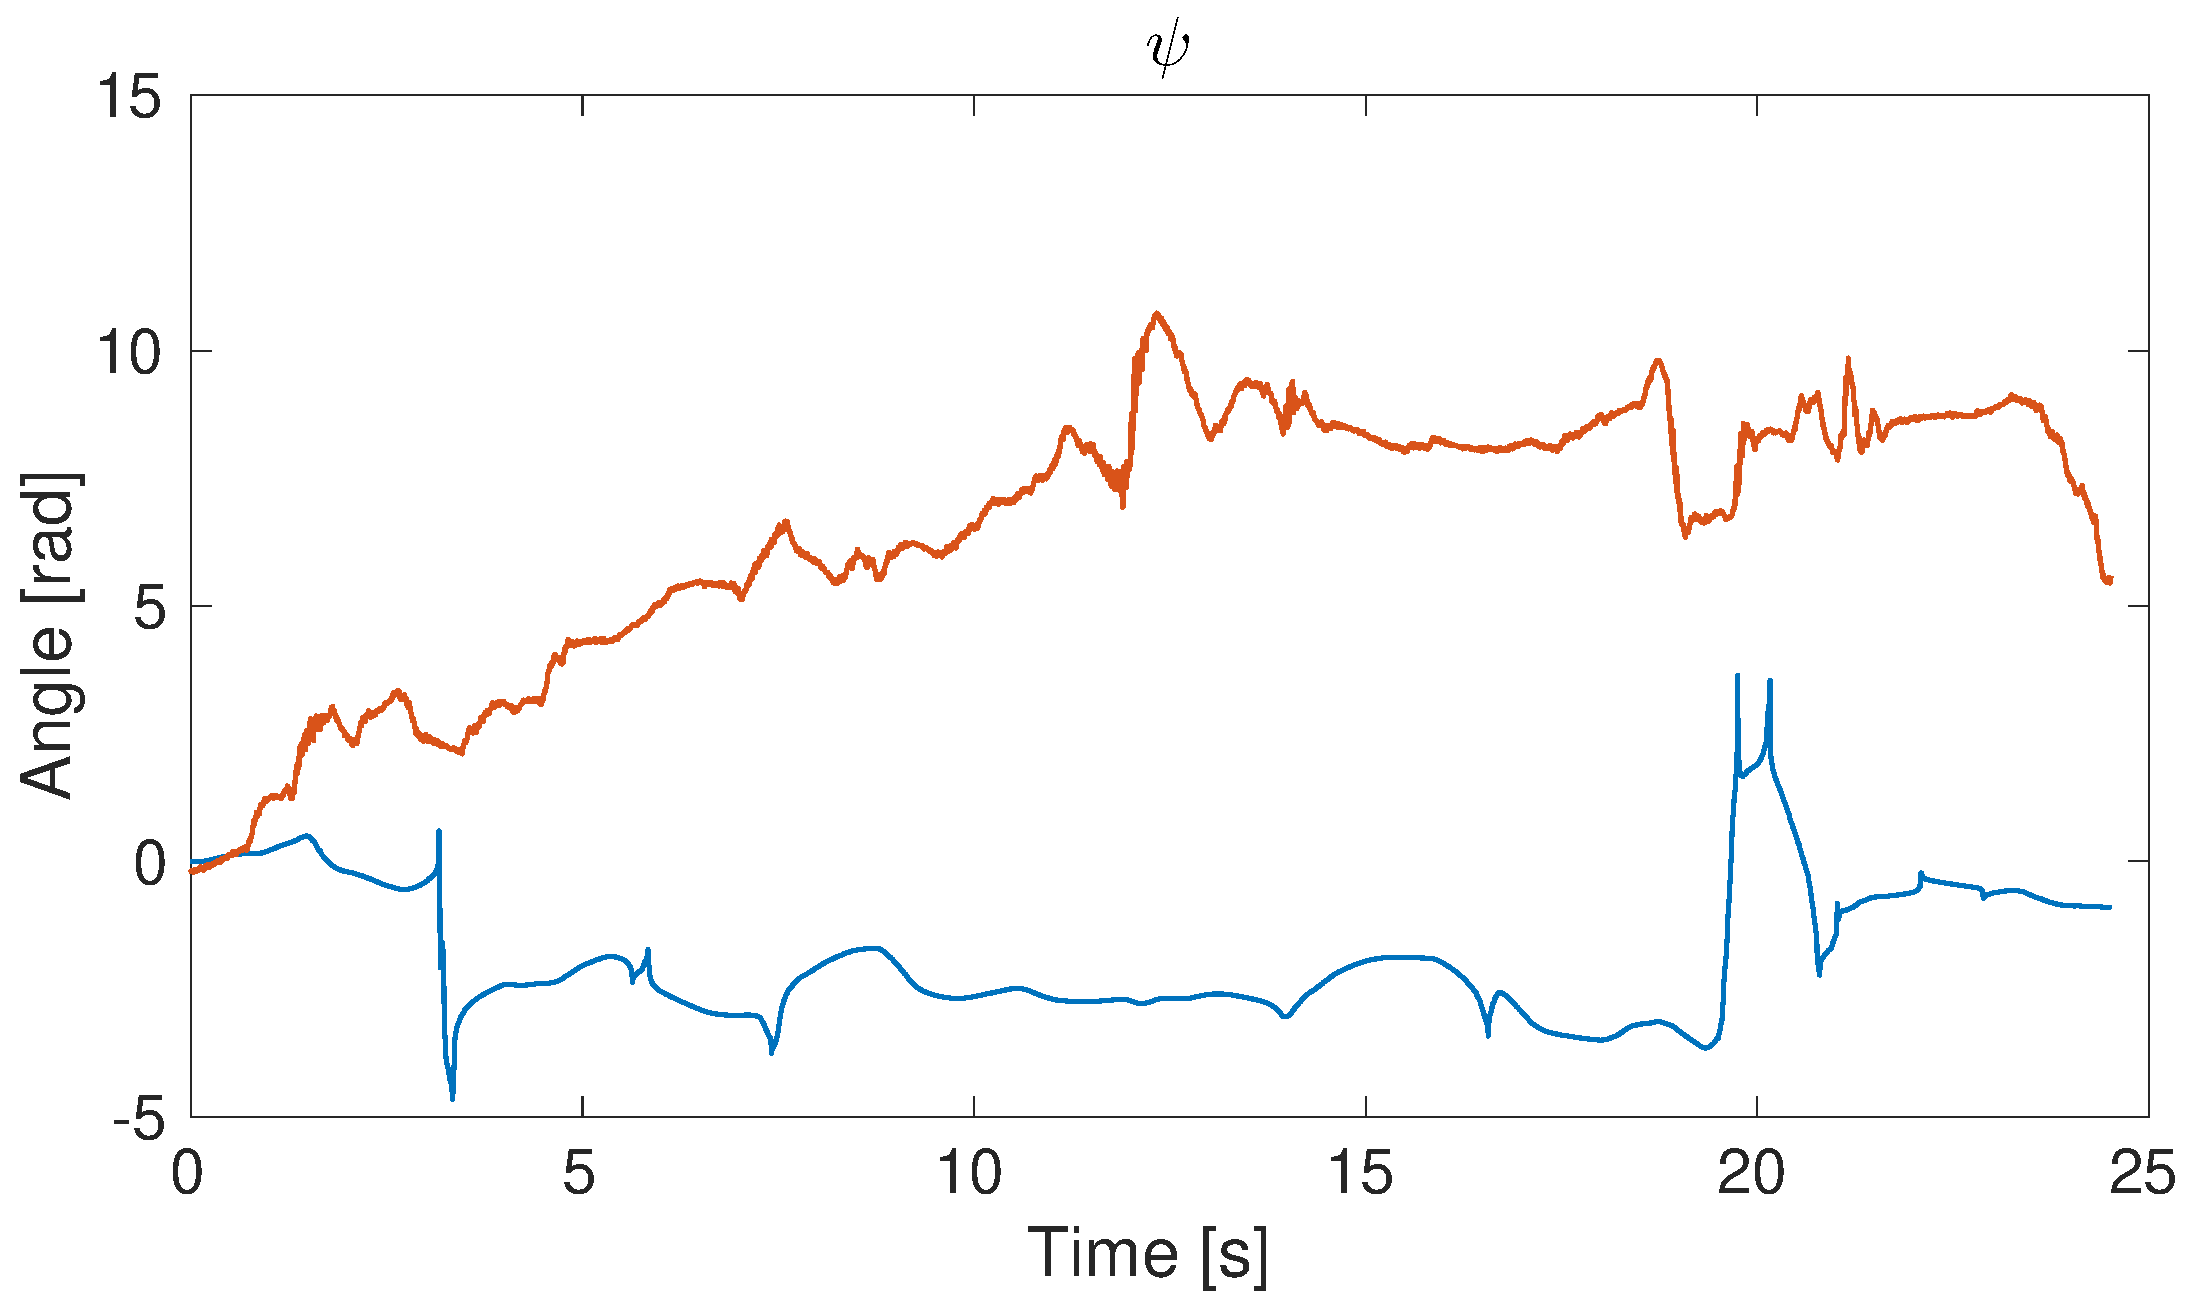
\includegraphics[width=0.4\textwidth]{velocityAnglePsi}}
  \caption{\label{fig:integratedAngleVelocities}%
  A comparison between integration of euler angles (blue) using \eqref{eq:eulerAnglesdot} and the estimated euler angles from the \abbrEKF (red). The angles are poorly estimated and thus not suitable to use as outputs in parameter estimation.}
\end{figure}
\index{Model structure}
Due to the aforementioned problems, the model \eqref{eq:quatModel} was used with angular velocities and linear acceleration as outputs. Thus the estimation structure became
\begin{equation}
\dot{\hat{\etaVector}} = J(\hat{\etaVector}) \hat{\nuVector},
\end{equation}
\begin{equation}
\dot{\hat{\nuVector}} =  f(\hat{\etaVector}, \hat{\nuVector}, \tauVector)
\end{equation}
with 
\begin{equation}
\hat{\boldsymbol{y}} = \begin{bmatrix}
\hat{\nuVector} \\
\hat{\boldsymbol{a}}
\end{bmatrix}
\end{equation}
where $\hat{\boldsymbol{a}}$ is the estimated linear acceleration in the \abbrROV frame. The measurement equation for $\boldsymbol{a}$ is
\begin{equation}
\boldsymbol{a} = \begin{bmatrix}
    2 g \quatO \quatII -2 g \quatI \quatIII \\
    -2 g \quatO \quatI -2g \quatII \quatIII \\
    2g \quatI^2 + 2 g \quatII^2 - g 
    \end{bmatrix}
\end{equation} 

An issue that was encountered when estimating the parameters was that when angular velocities and linear accelerations were used as outputs, the model was extremely sensitive to the initial value of the quaternions. To examine this problem further, data was generated using a simulator and the simulated data was used in the estimation. The estimator was initialised with the correct initial parameter values from the simulator, but it was free to estimate the initial value of the quaternions. As expected, the estimated starting quaternion was not well estimated, which in turn led to the parameters diverging from their true values and a low fit was obtained. A result from such a test can be seen in \Figureref{fig:angVelSim}.

\begin{figure}[htbp]
  \centering %comparison betwwen two simulations
  \subfloat[][\label{fig:angVelSimp}Angular velocity around the \abbrROV's x-axis.]{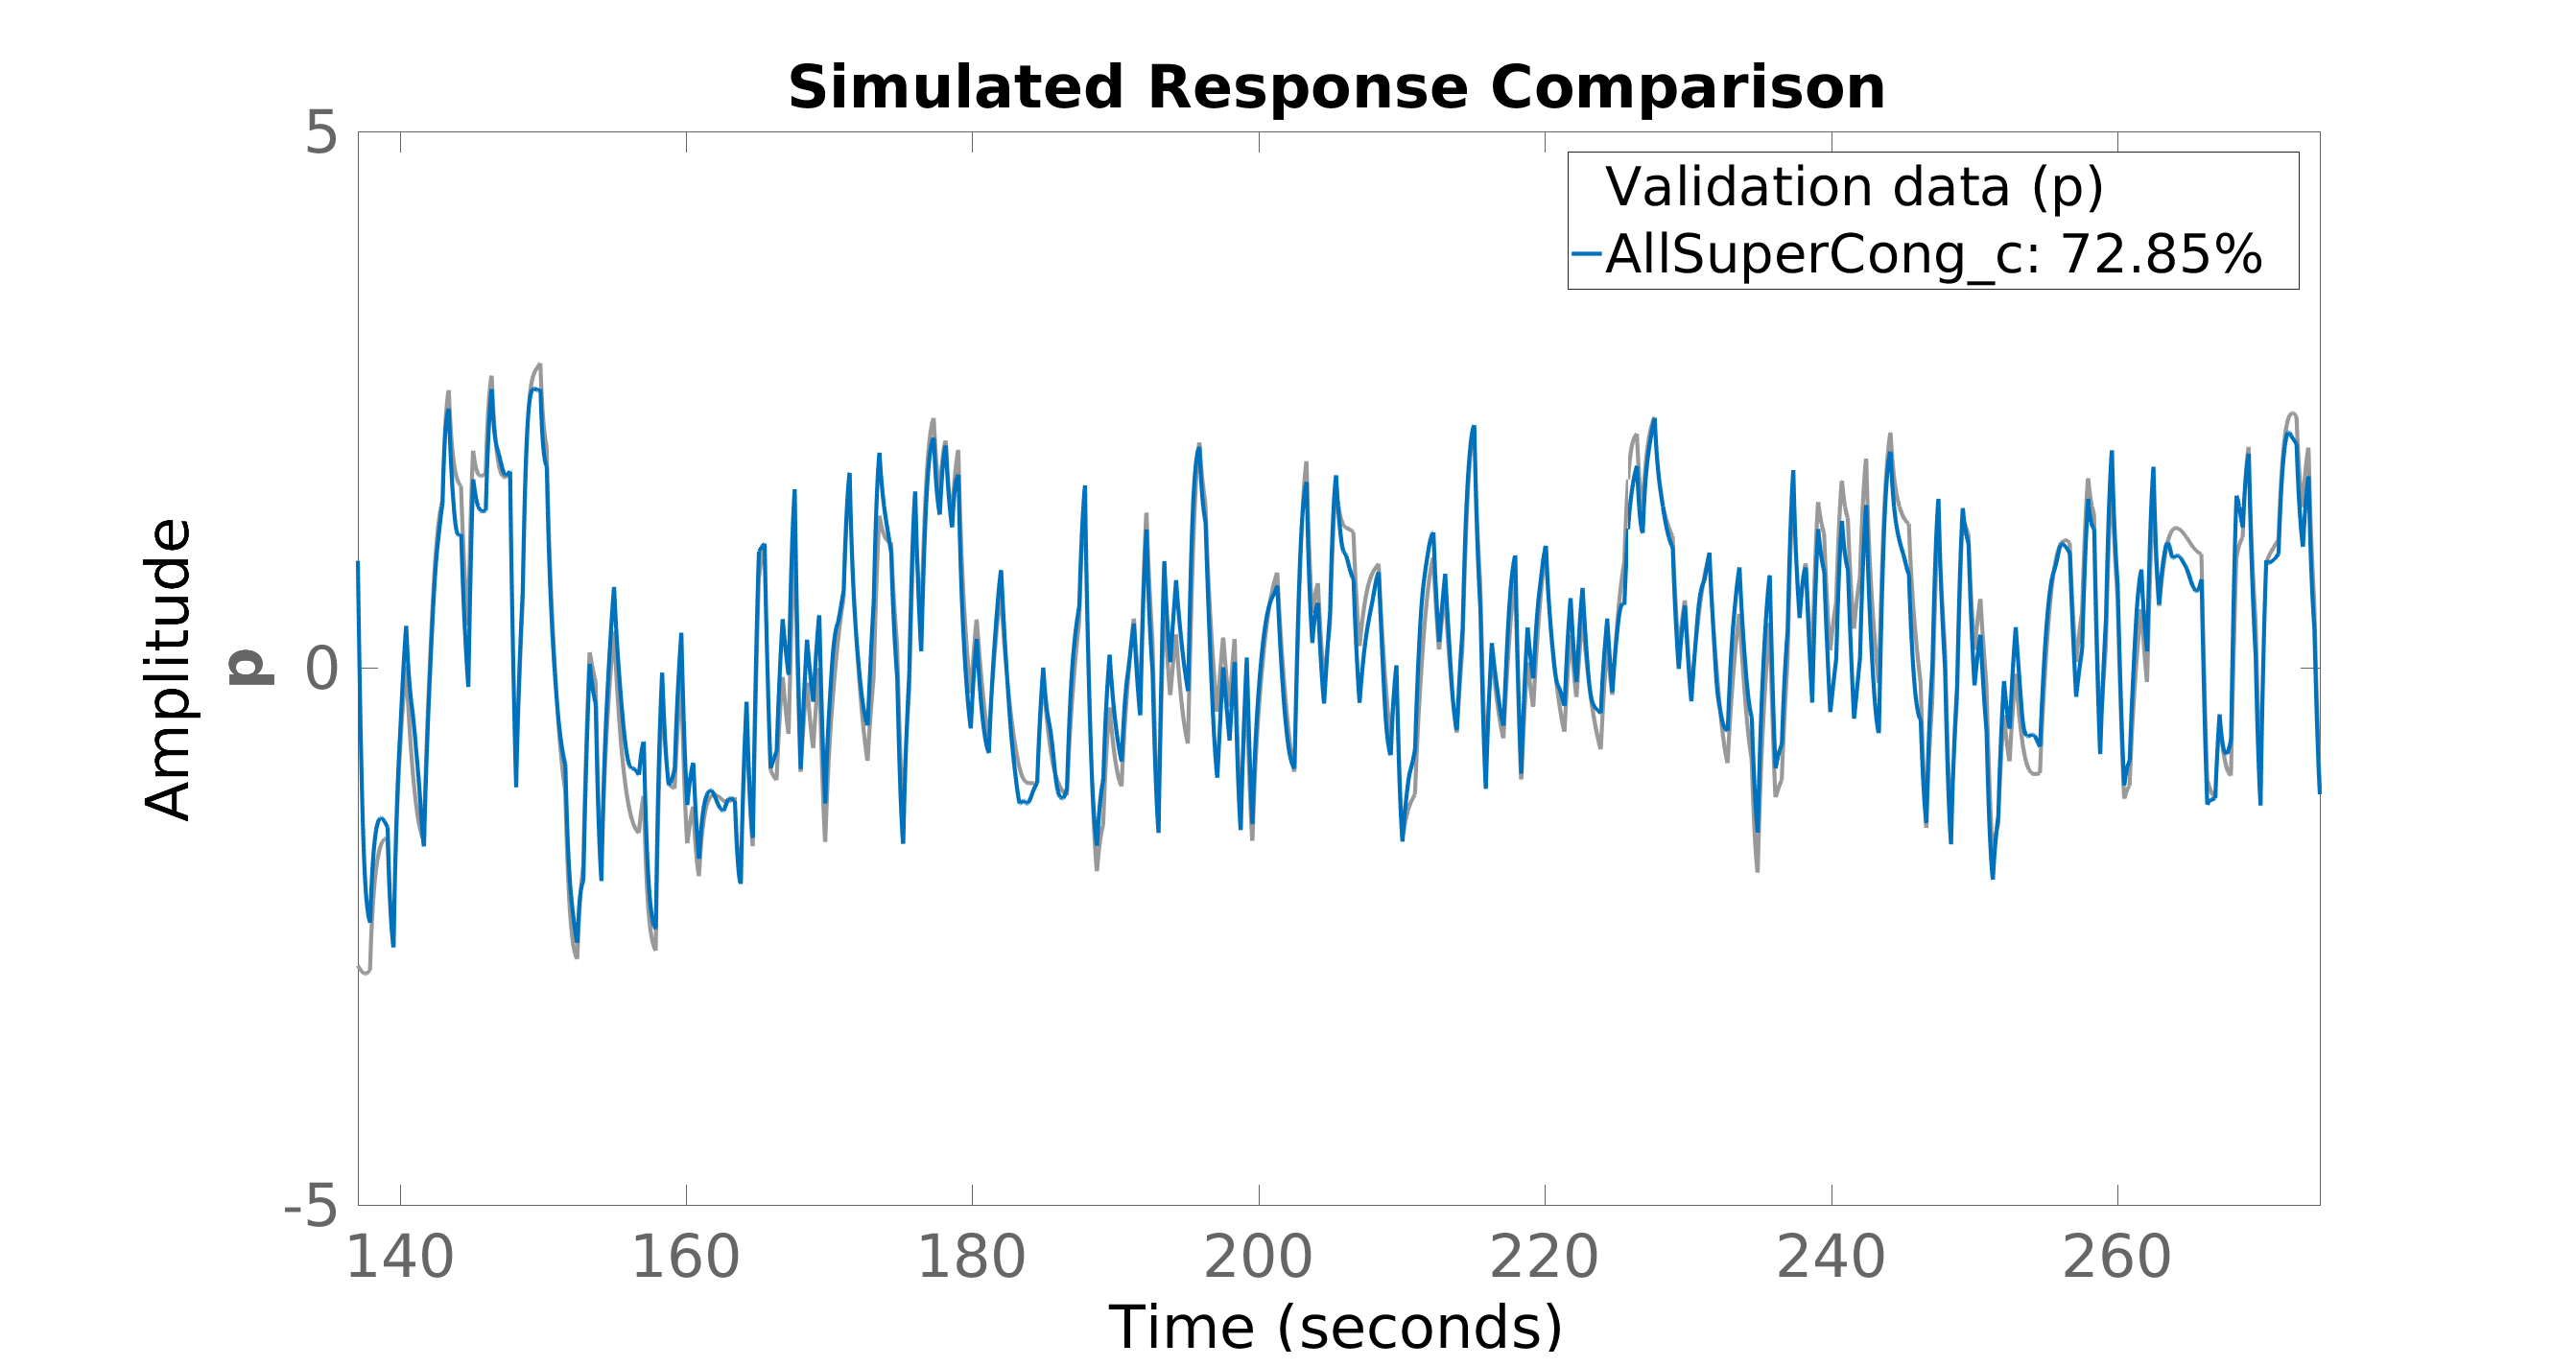
\includegraphics[width=0.4\textwidth]{angVelSimp}}
  \qquad
  \subfloat[][\label{fig:angVelSimq}Angular velocity around the \abbrROV's y-axis.]{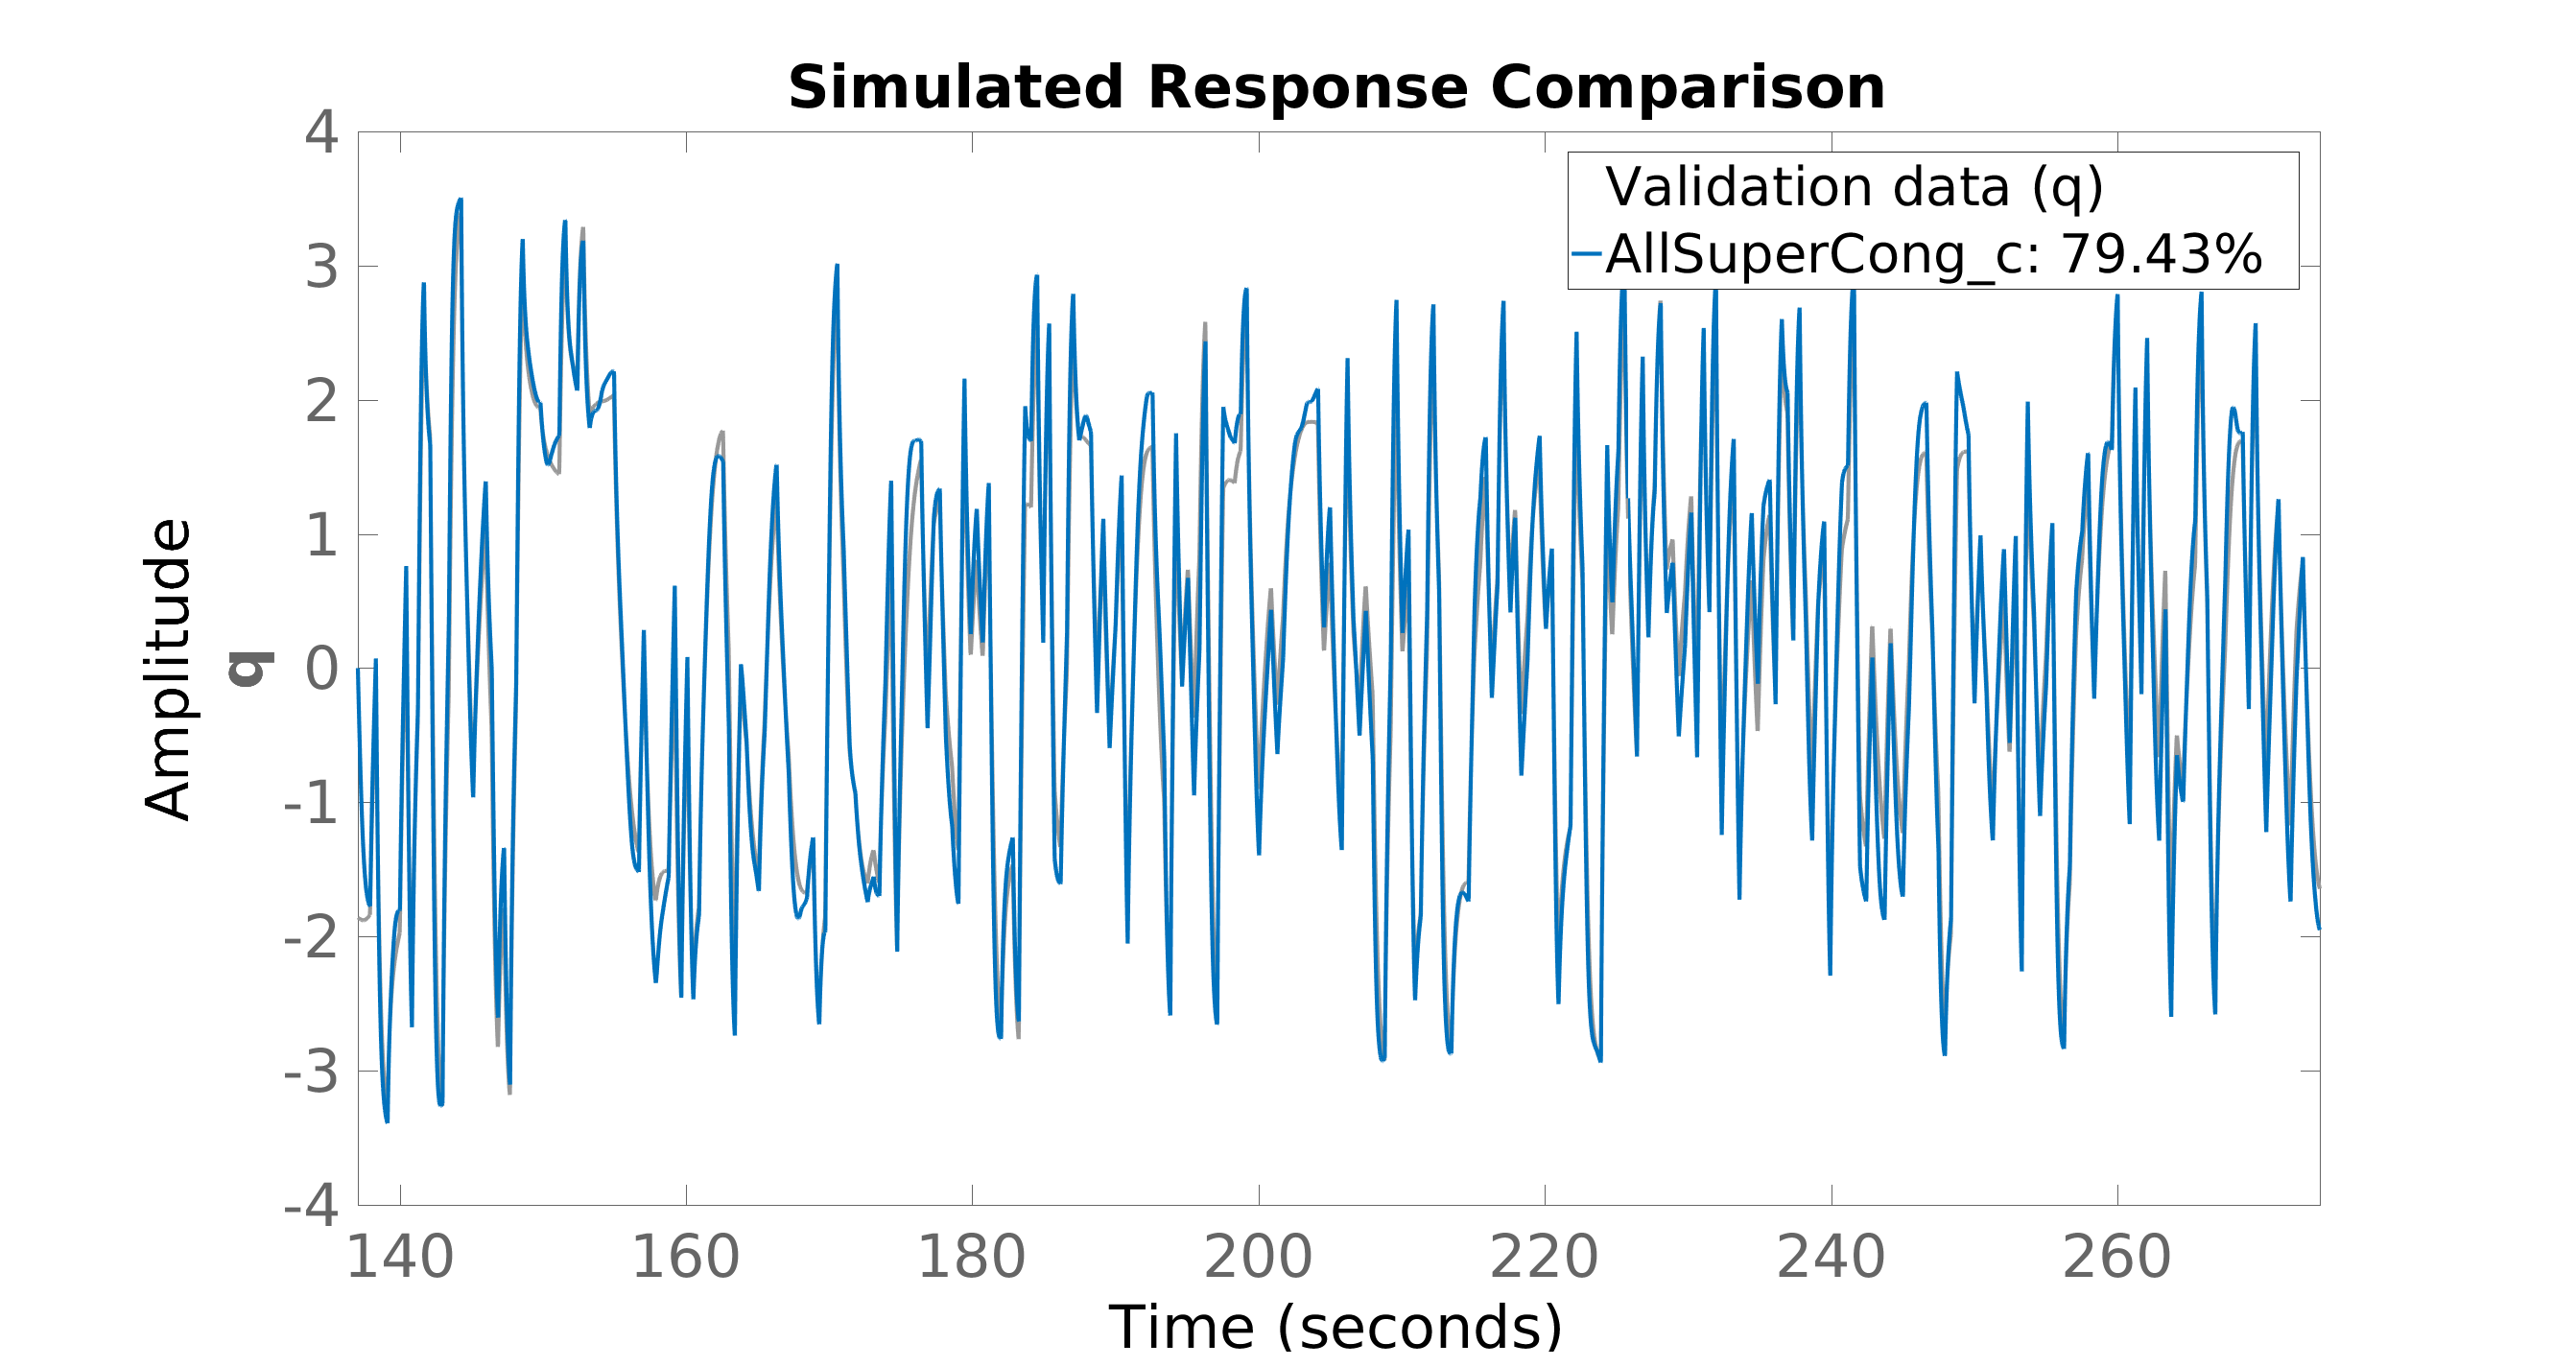
\includegraphics[width=0.4\textwidth]{angVelSimq}}
  \qquad
  \subfloat[][\label{fig:angVelSimr}Angular velocity around the \abbrROV's z-axis.]{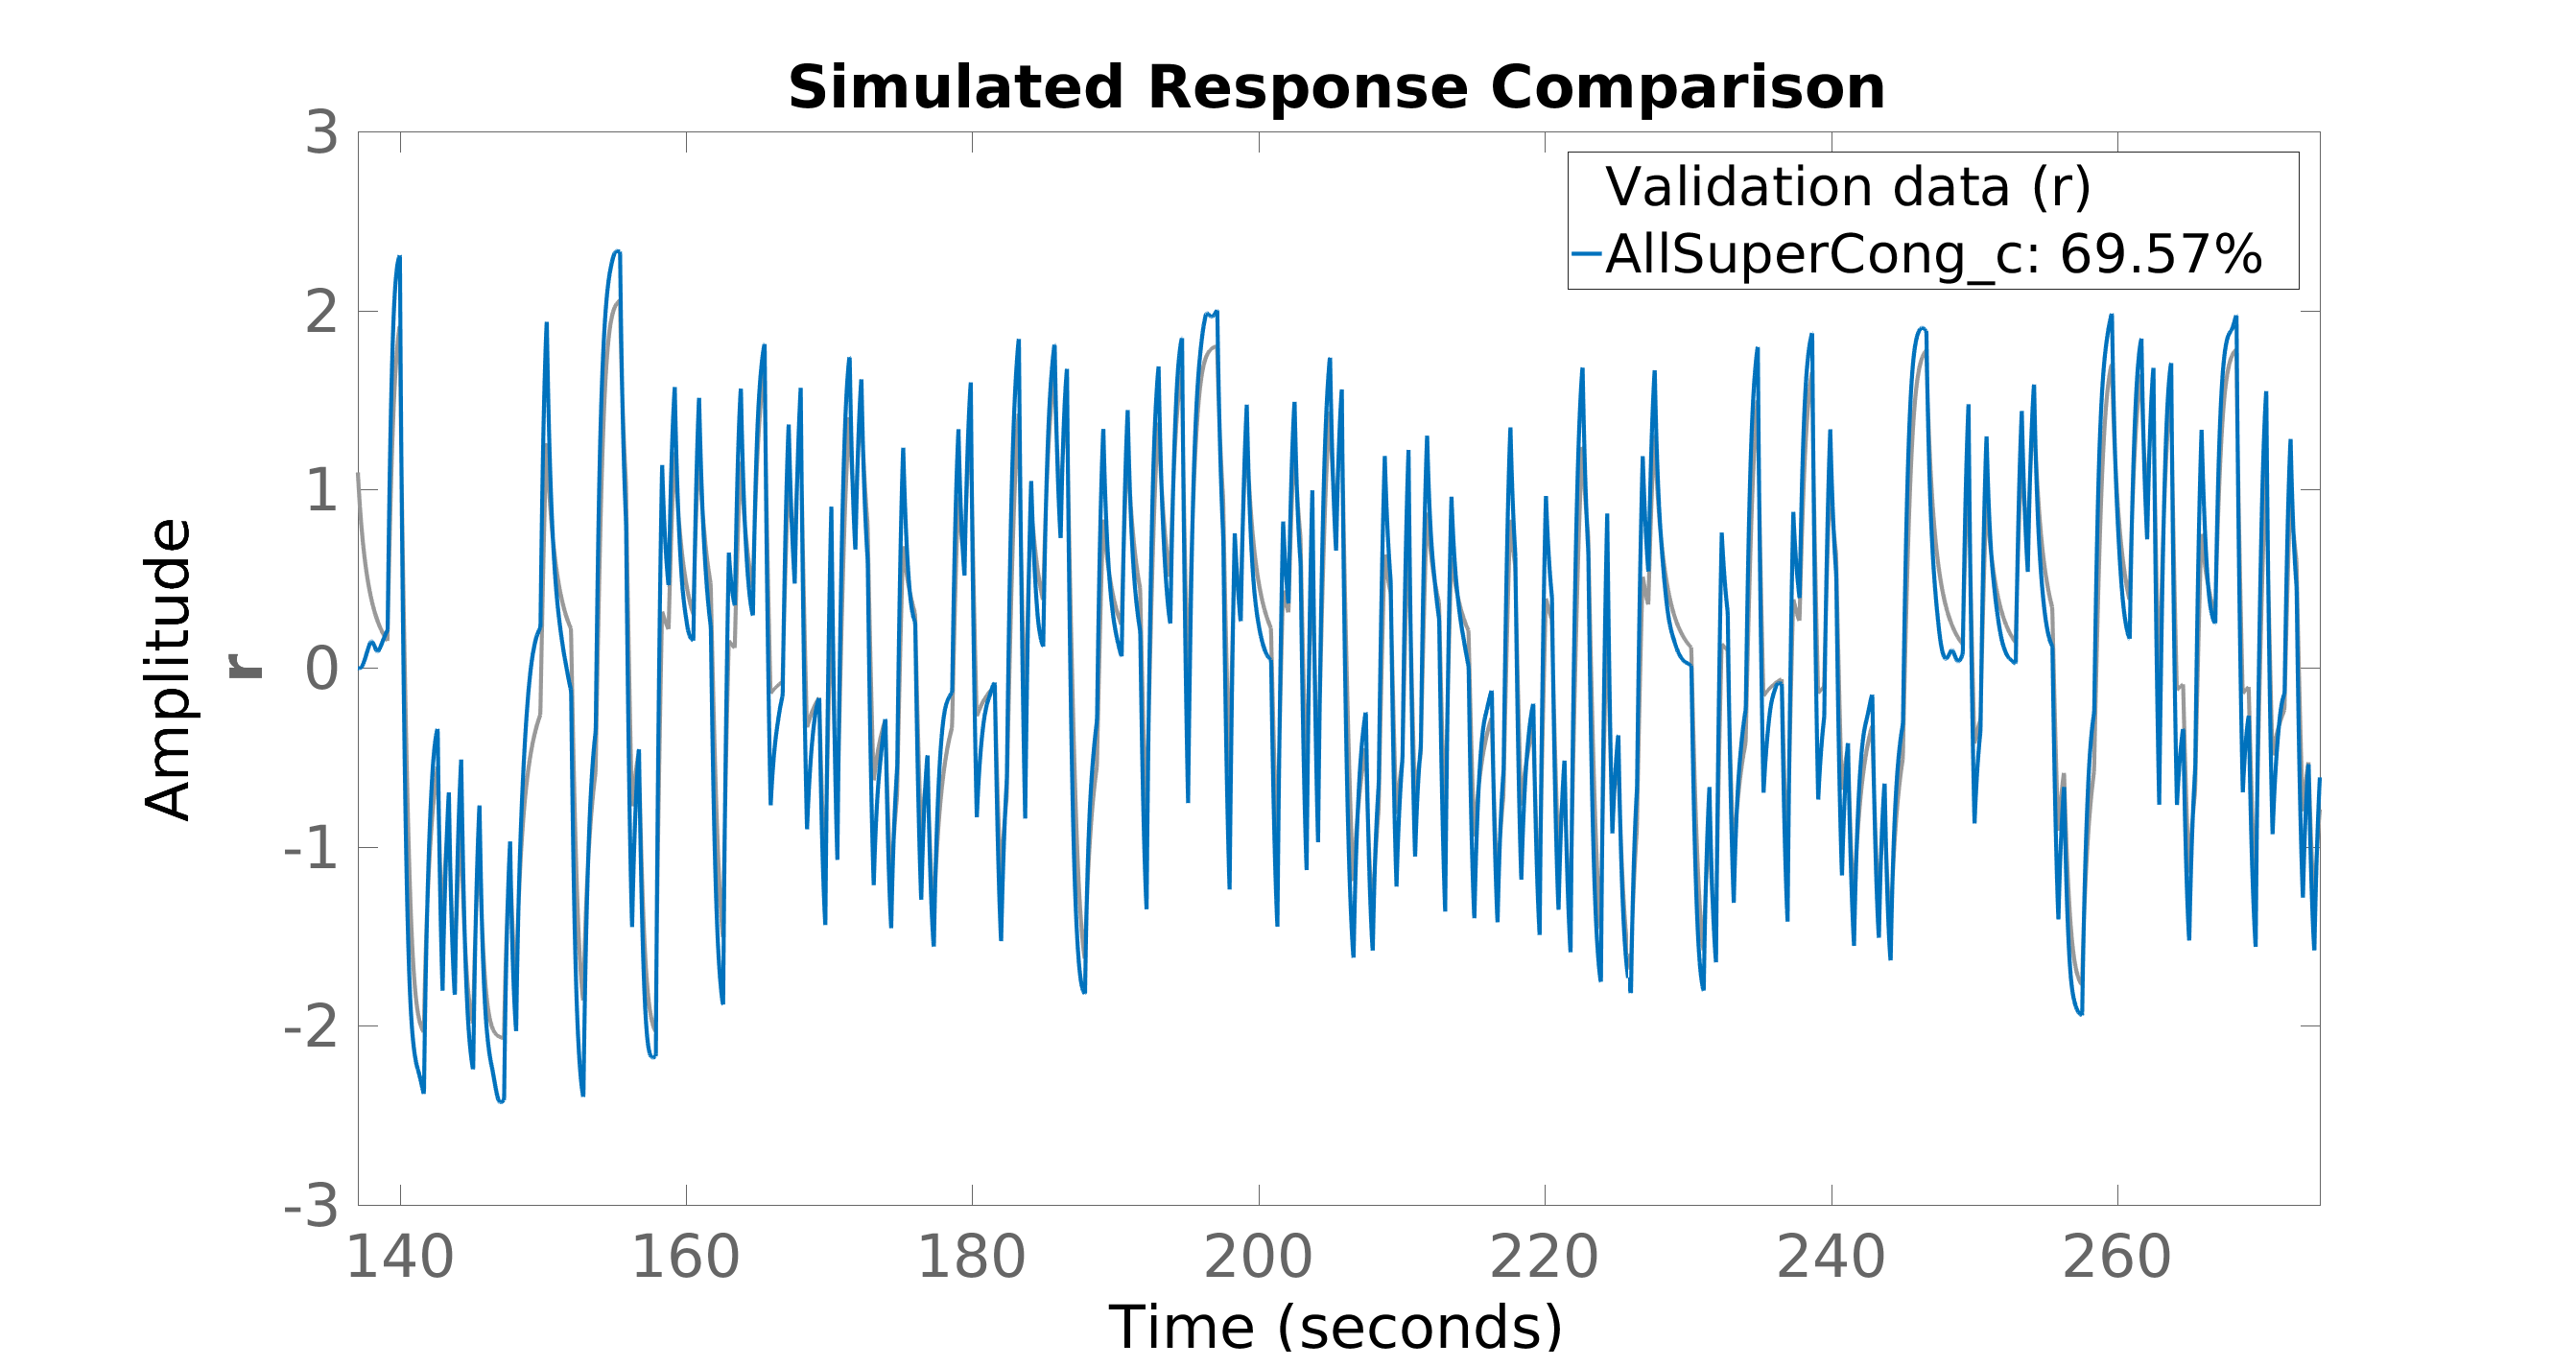
\includegraphics[width=0.4\textwidth]{angVelSimr}}
    \qquad
  \subfloat[][\label{fig:linAccSimx}Linear acceleration in the \abbrROV's x-axis.]{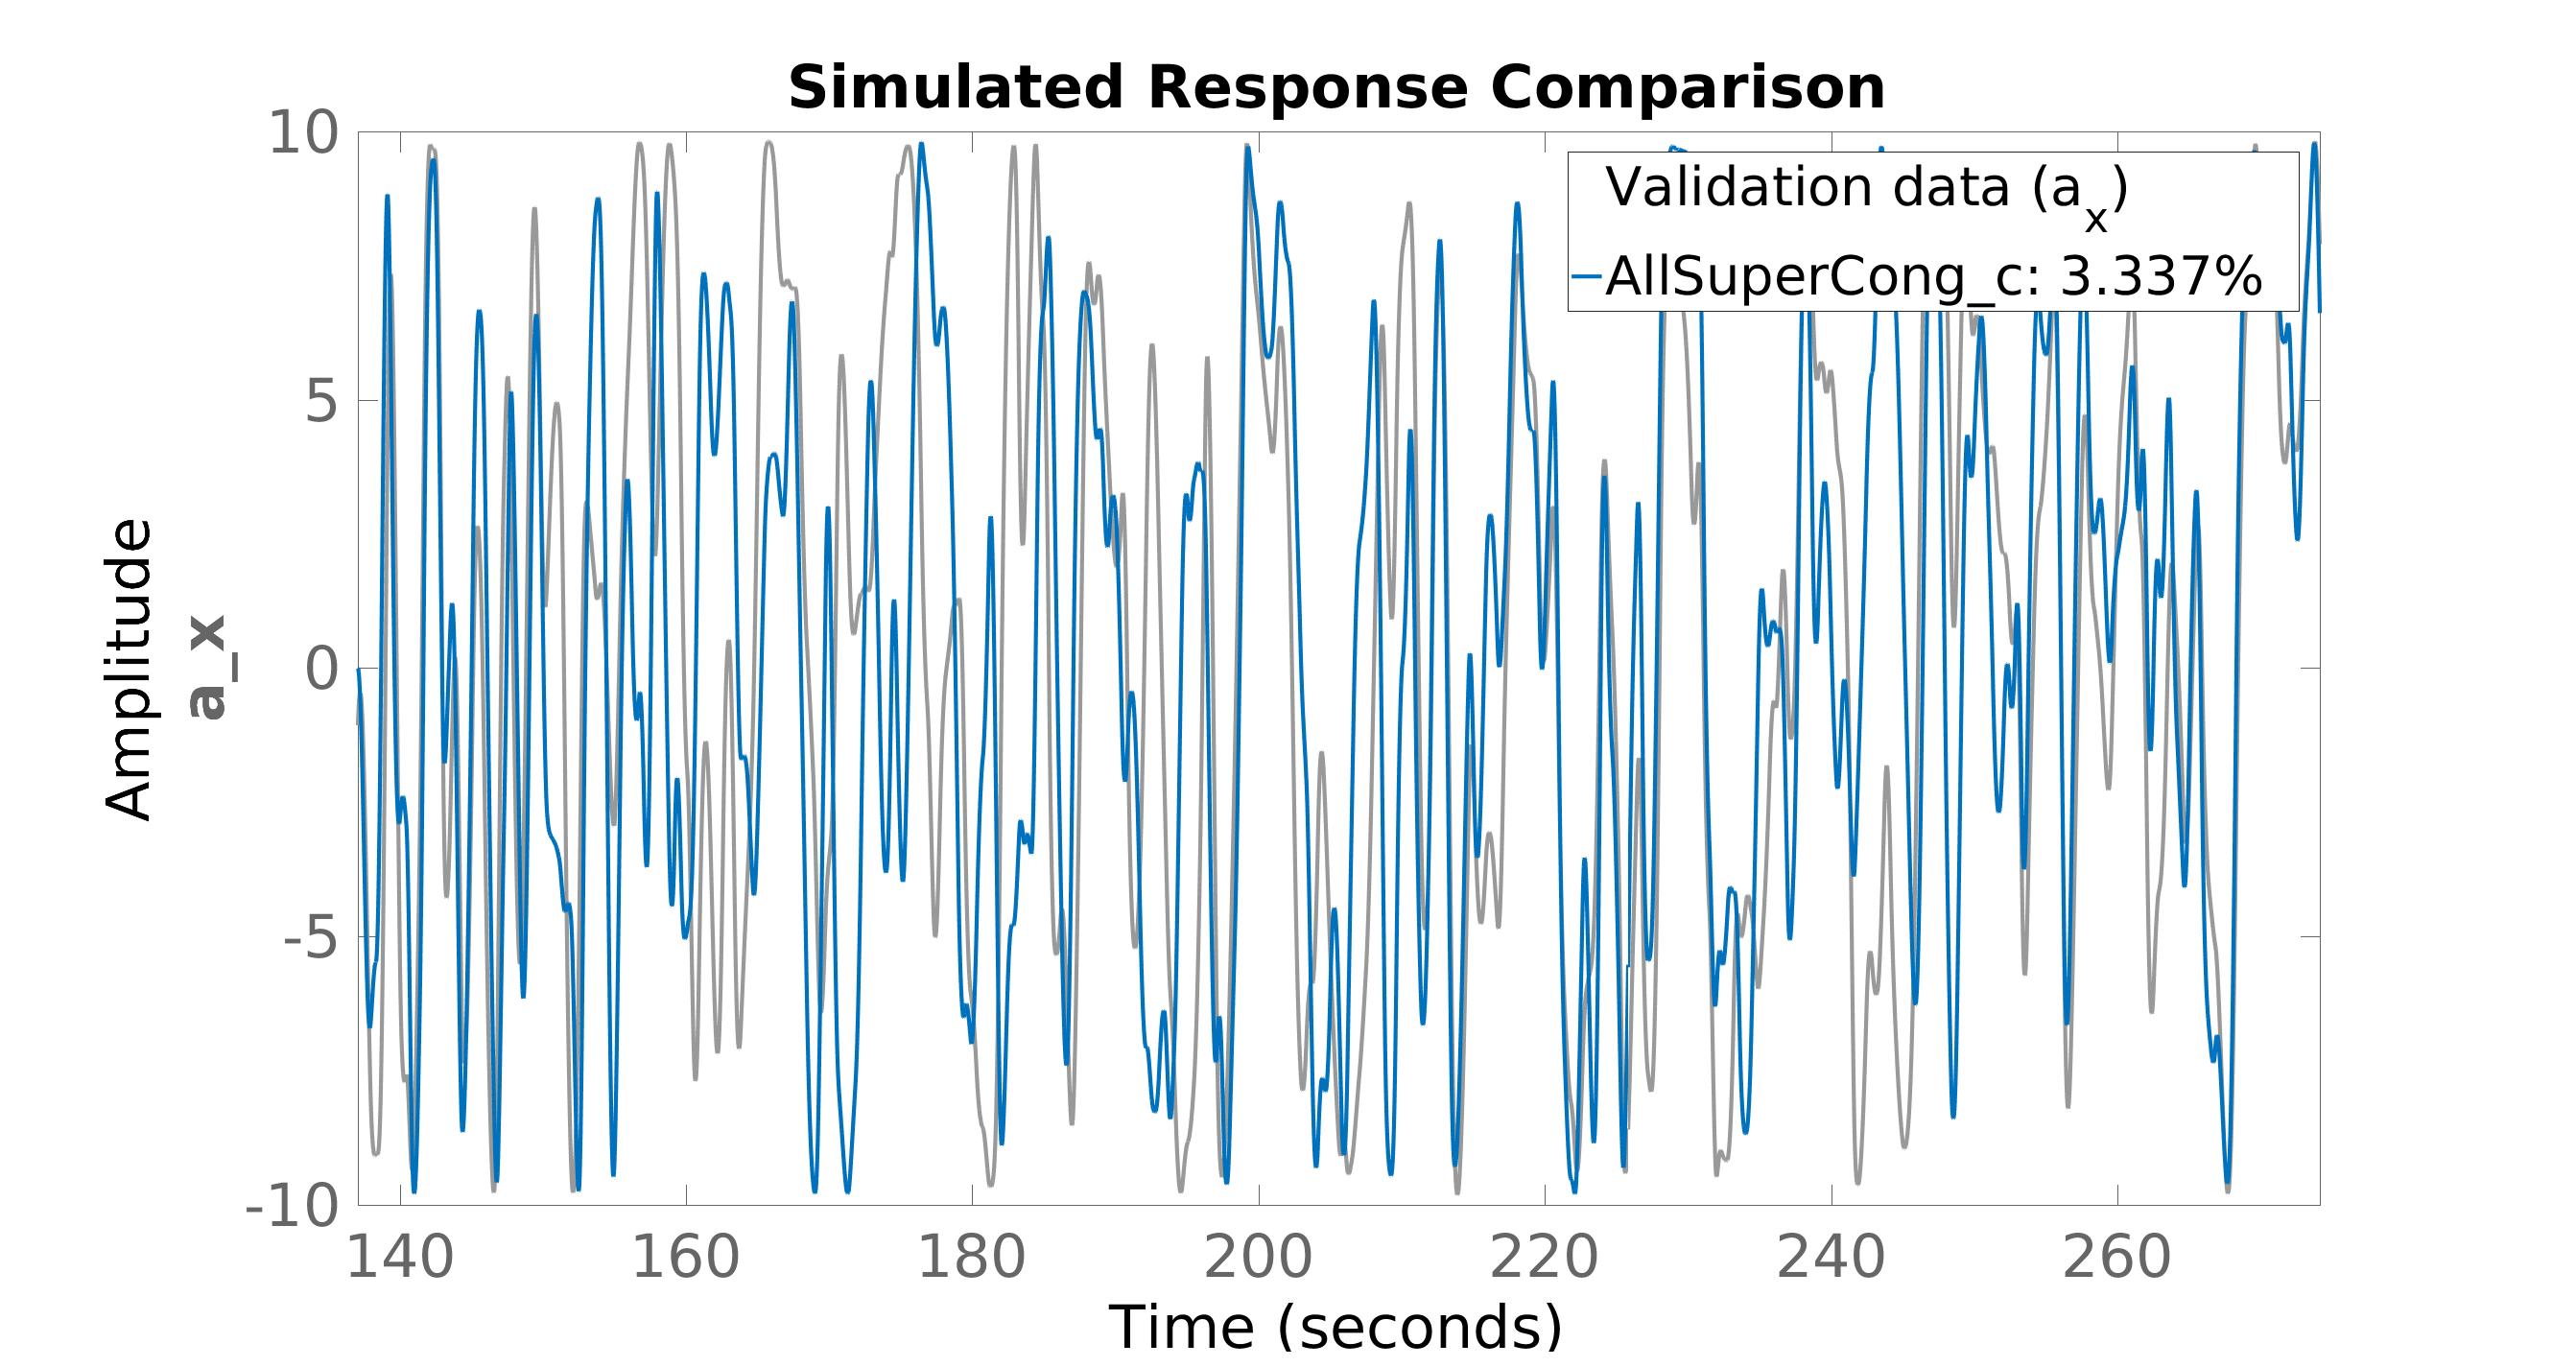
\includegraphics[width=0.4\textwidth]{linAccSimx}}
    \qquad
  \subfloat[][\label{fig:linAccSimy}Linear acceleration in the \abbrROV's y-axis.]{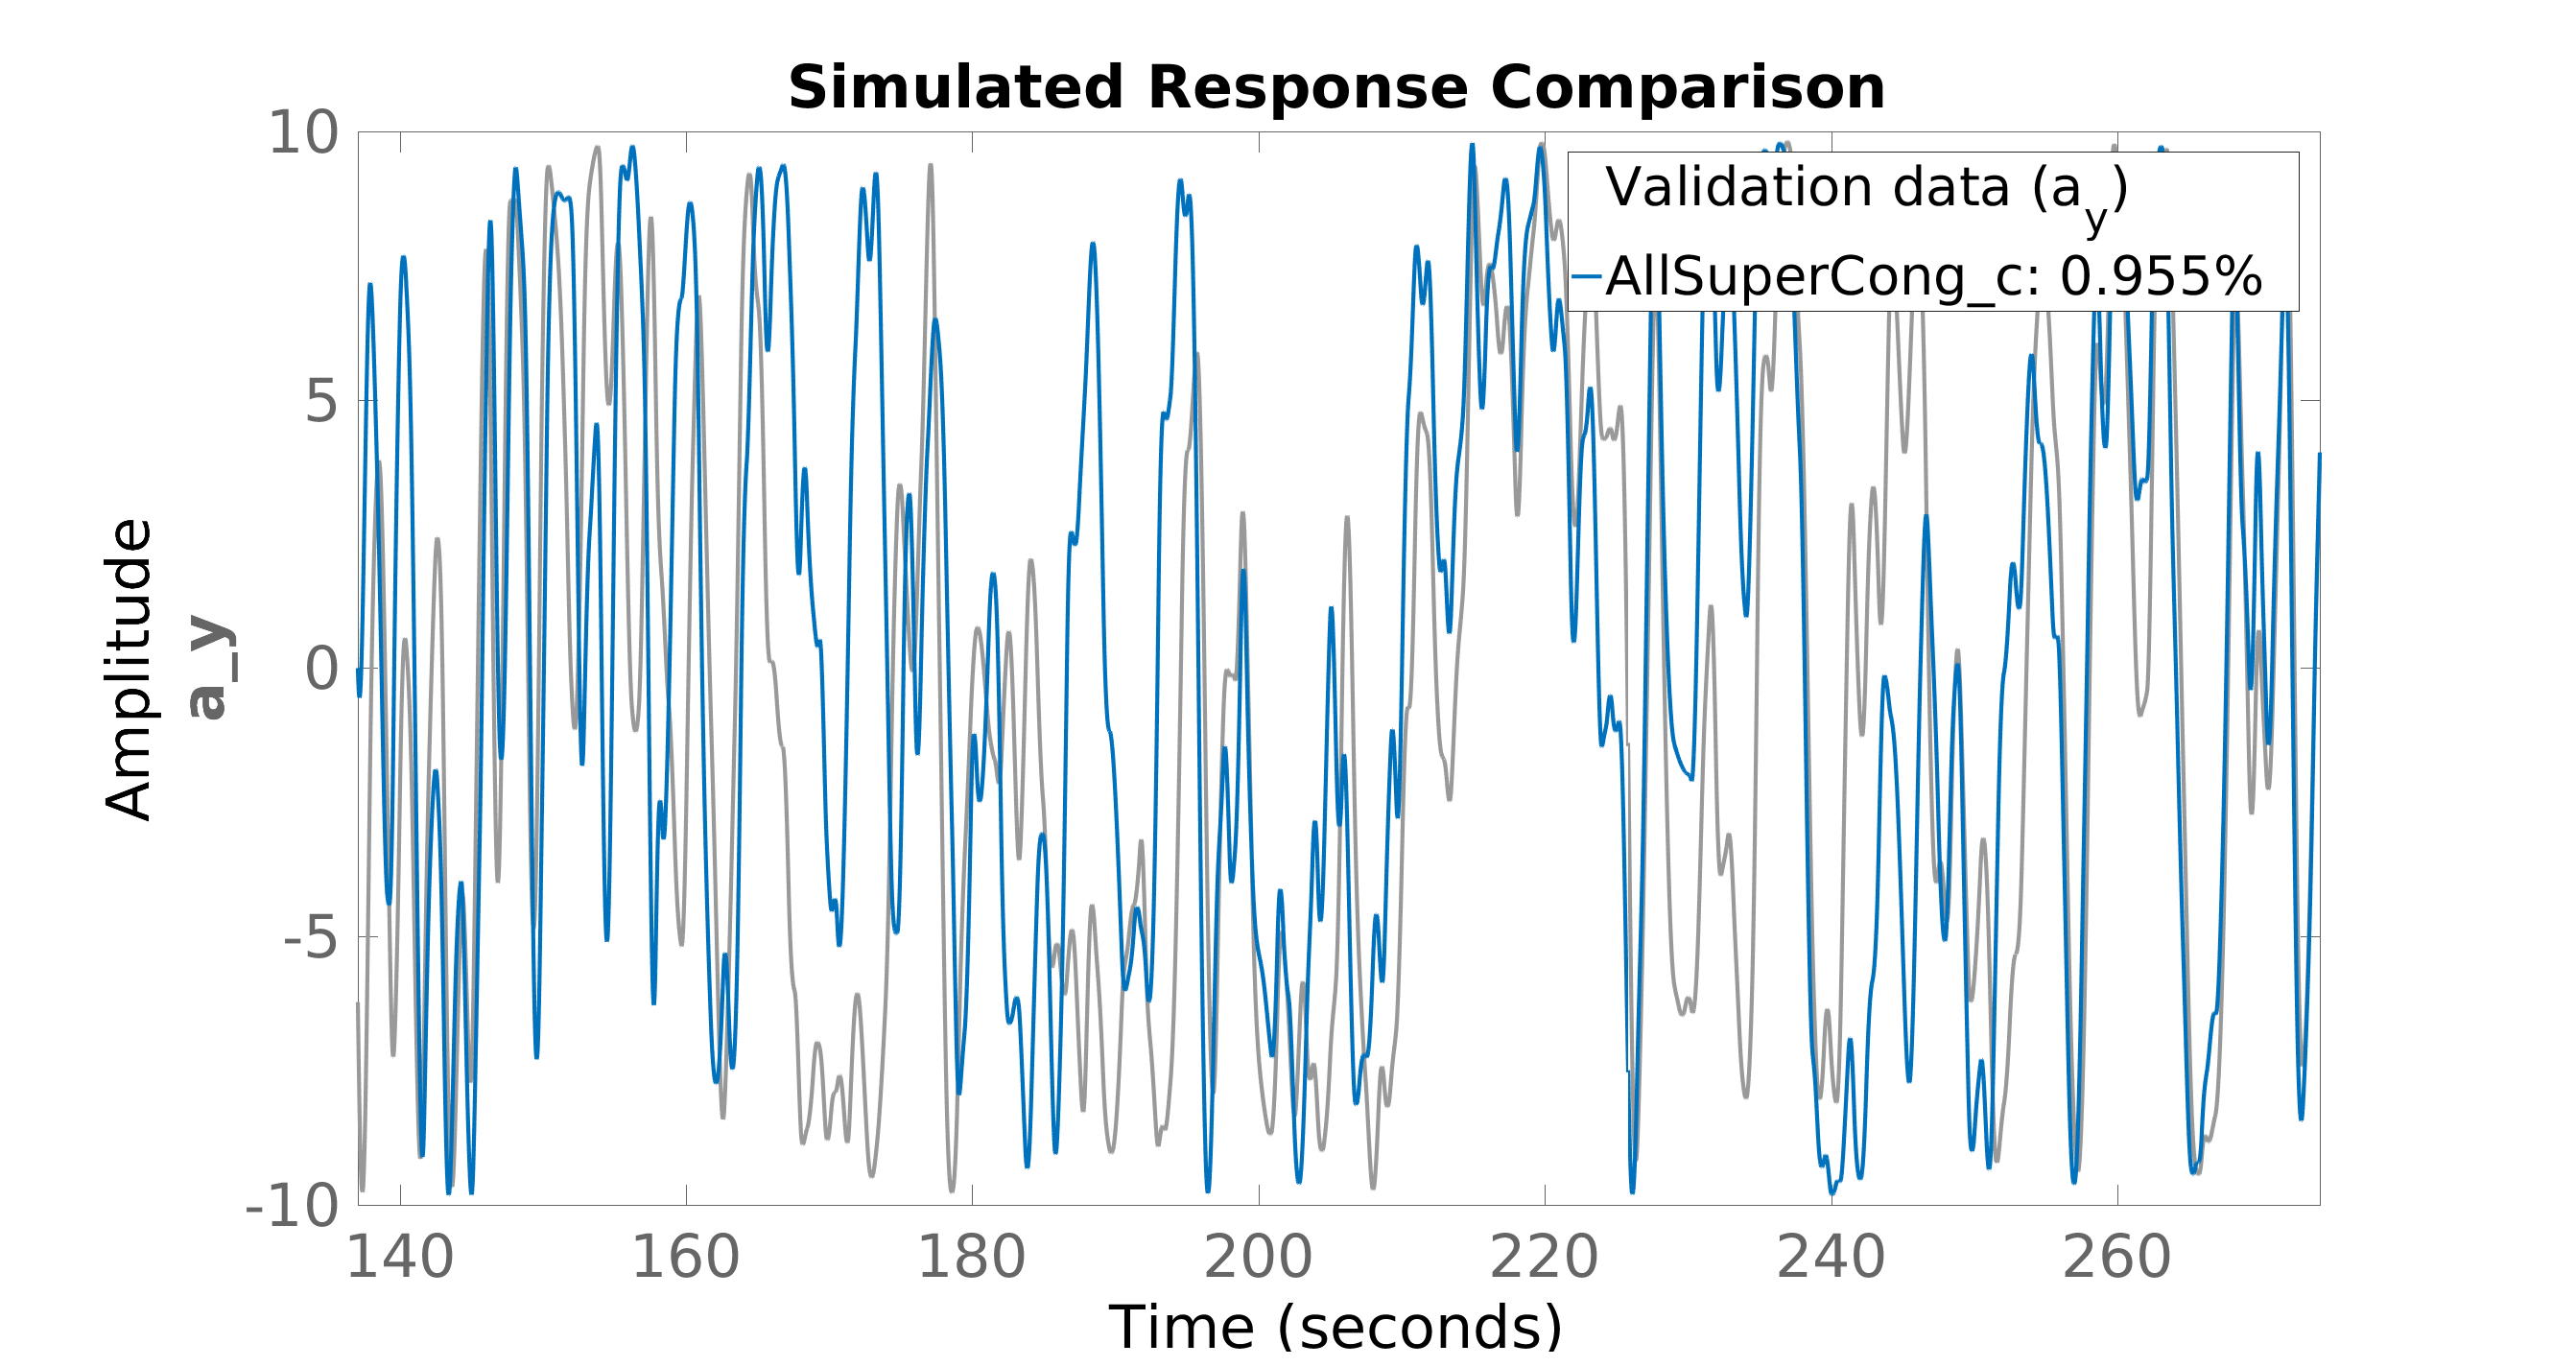
\includegraphics[width=0.4\textwidth]{linAccSimy}}
    \qquad
  \subfloat[][\label{fig:linAccSimz}Linear acceleration  in the \abbrROV's z-axis.]{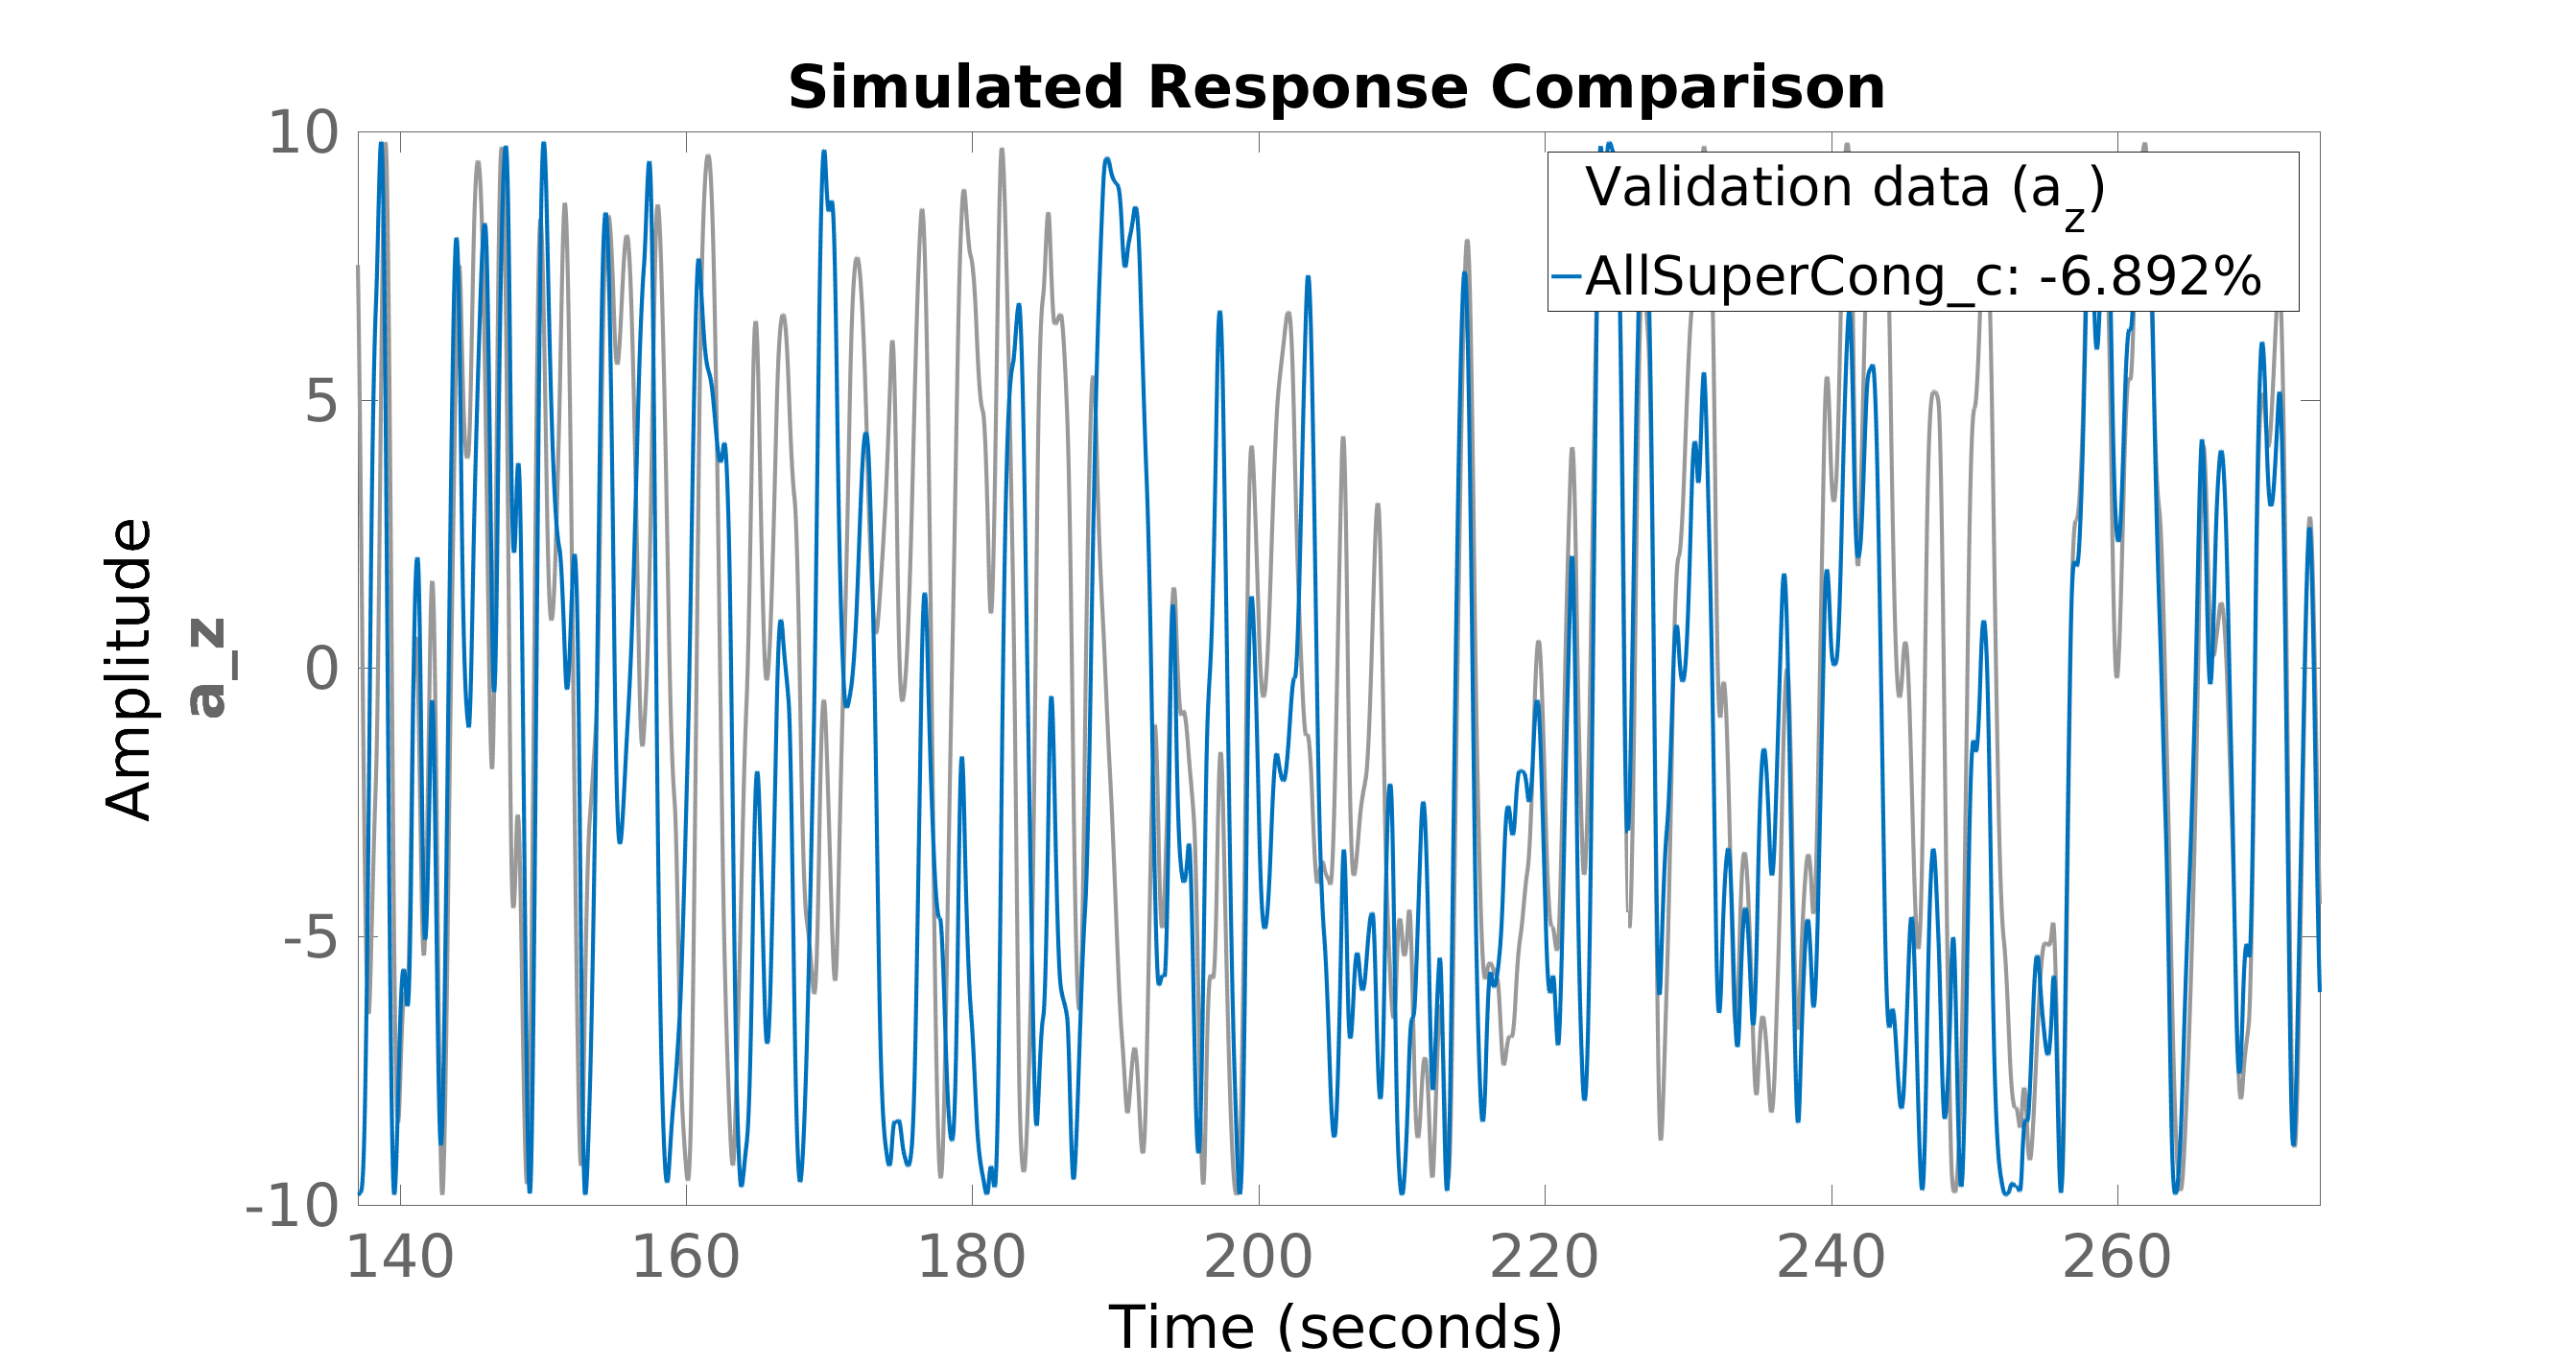
\includegraphics[width=0.4\textwidth]{linAccSimz}}
  \caption{\label{fig:angVelSim}%
    Comparison between simulated validation data (grey) and the simulated response from the estimated model (blue). The fit for the model in each state is stated in each plot. The validation data has been generated using the initial parameters used in the parameter estimation. The poor initial state estimate results in that the estimated parameters diverge from their true values.}
\end{figure}\index{Fit} \index{Model structure} \index{Quaternions}

To estimate the initial state of the quaternions, a Kalman smoother as described in \citet{Wallin} was used. The magnetometer was also added as an output, in the Kalman smoother, to further reduce the uncertainty of the initial quaternions. It is therefore recommended that attitude data is logged on quaternion form so that the initial quaternions can easily be obtained during parameter estimation. An alternative is that the \abbrROV's initial attitude is known. 

The estimated parameter values obtained when using \eqref{eq:quatModel} with angular velocities and linear accelerations as inputs can be seen in \Tableref{tab:ResultEstimAngular}. The fit of the model using the estimated parameters can be seen in \Figureref{fig:angVelComparelz6}. The high fit of $50\ \%$ in $q$ and $r$ means that the model describes parts of the validation data well. The model did not describe the linear accelerations and $p$ well, which can be seen in the low fit.

\begin{figure}[tbp]
  \centering
  \subfloat[][\label{fig:angVelCompareplz6}Angular velocity around the \abbrROV's x-axis.]{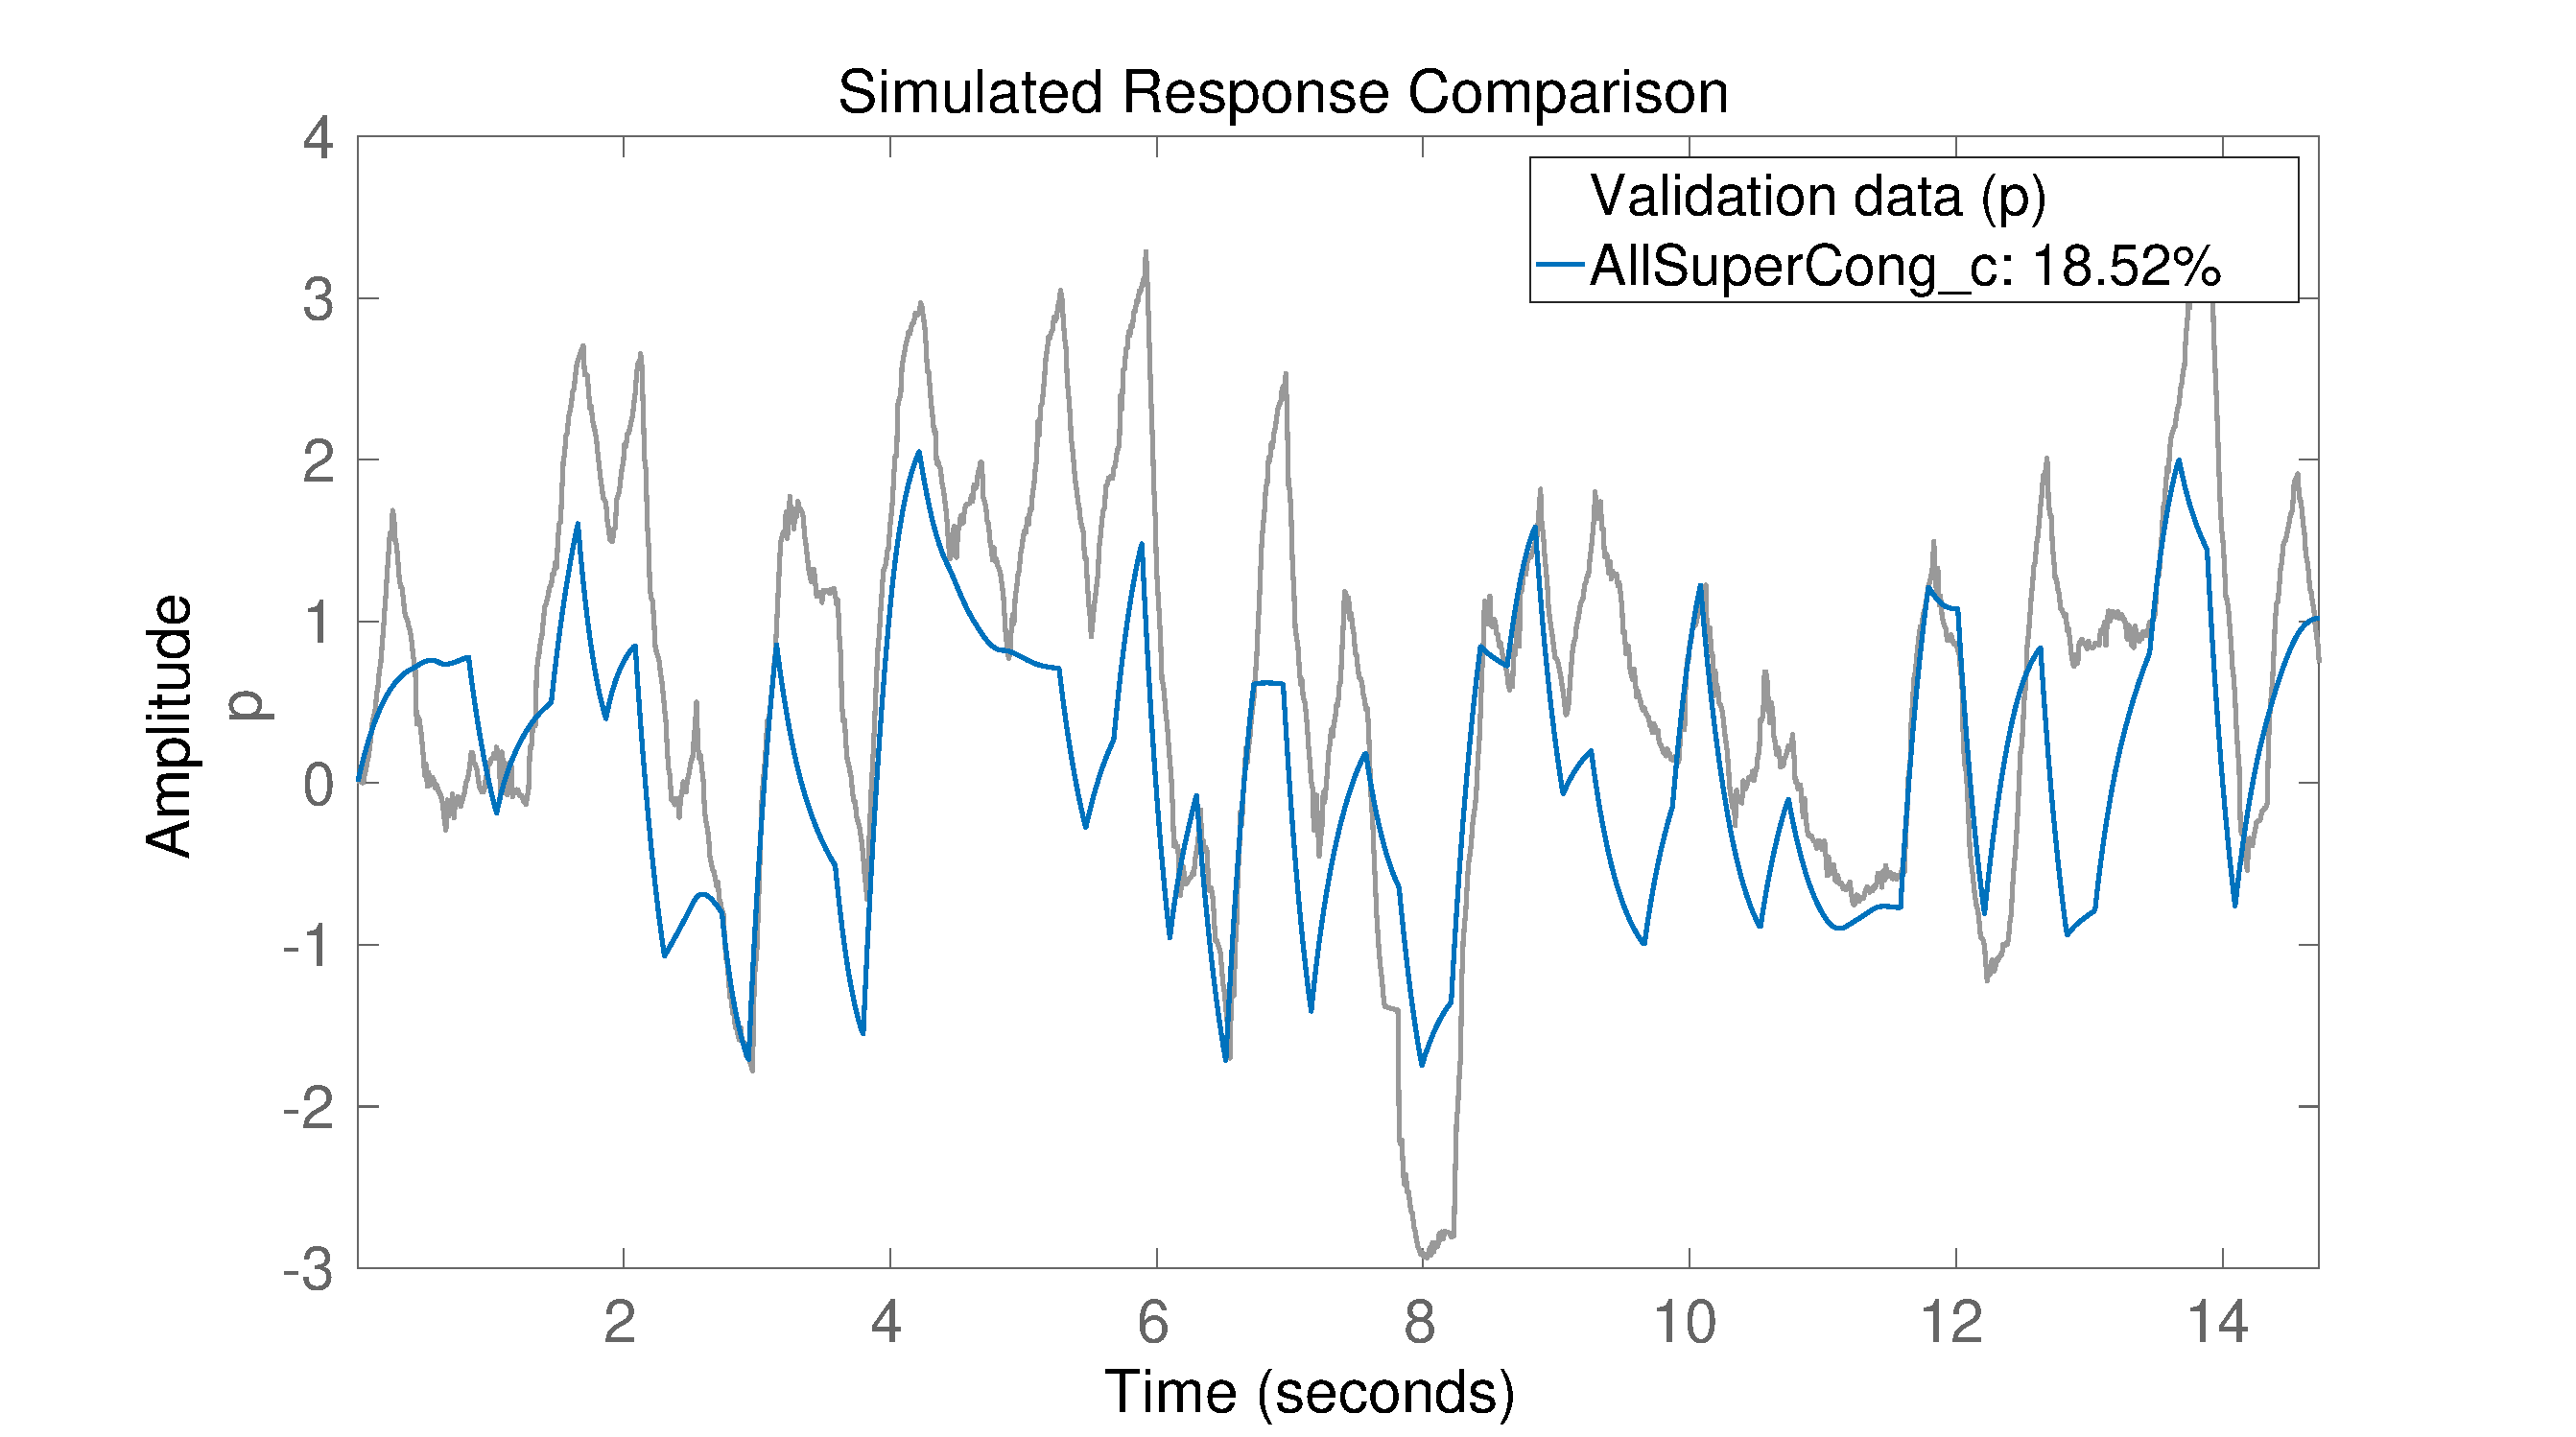
\includegraphics[width=0.4\textwidth]{angVelCompareplz6}}
  \qquad
  \subfloat[][\label{fig:angVelCompareqlz6}Angular velocity around the \abbrROV's y-axis.]{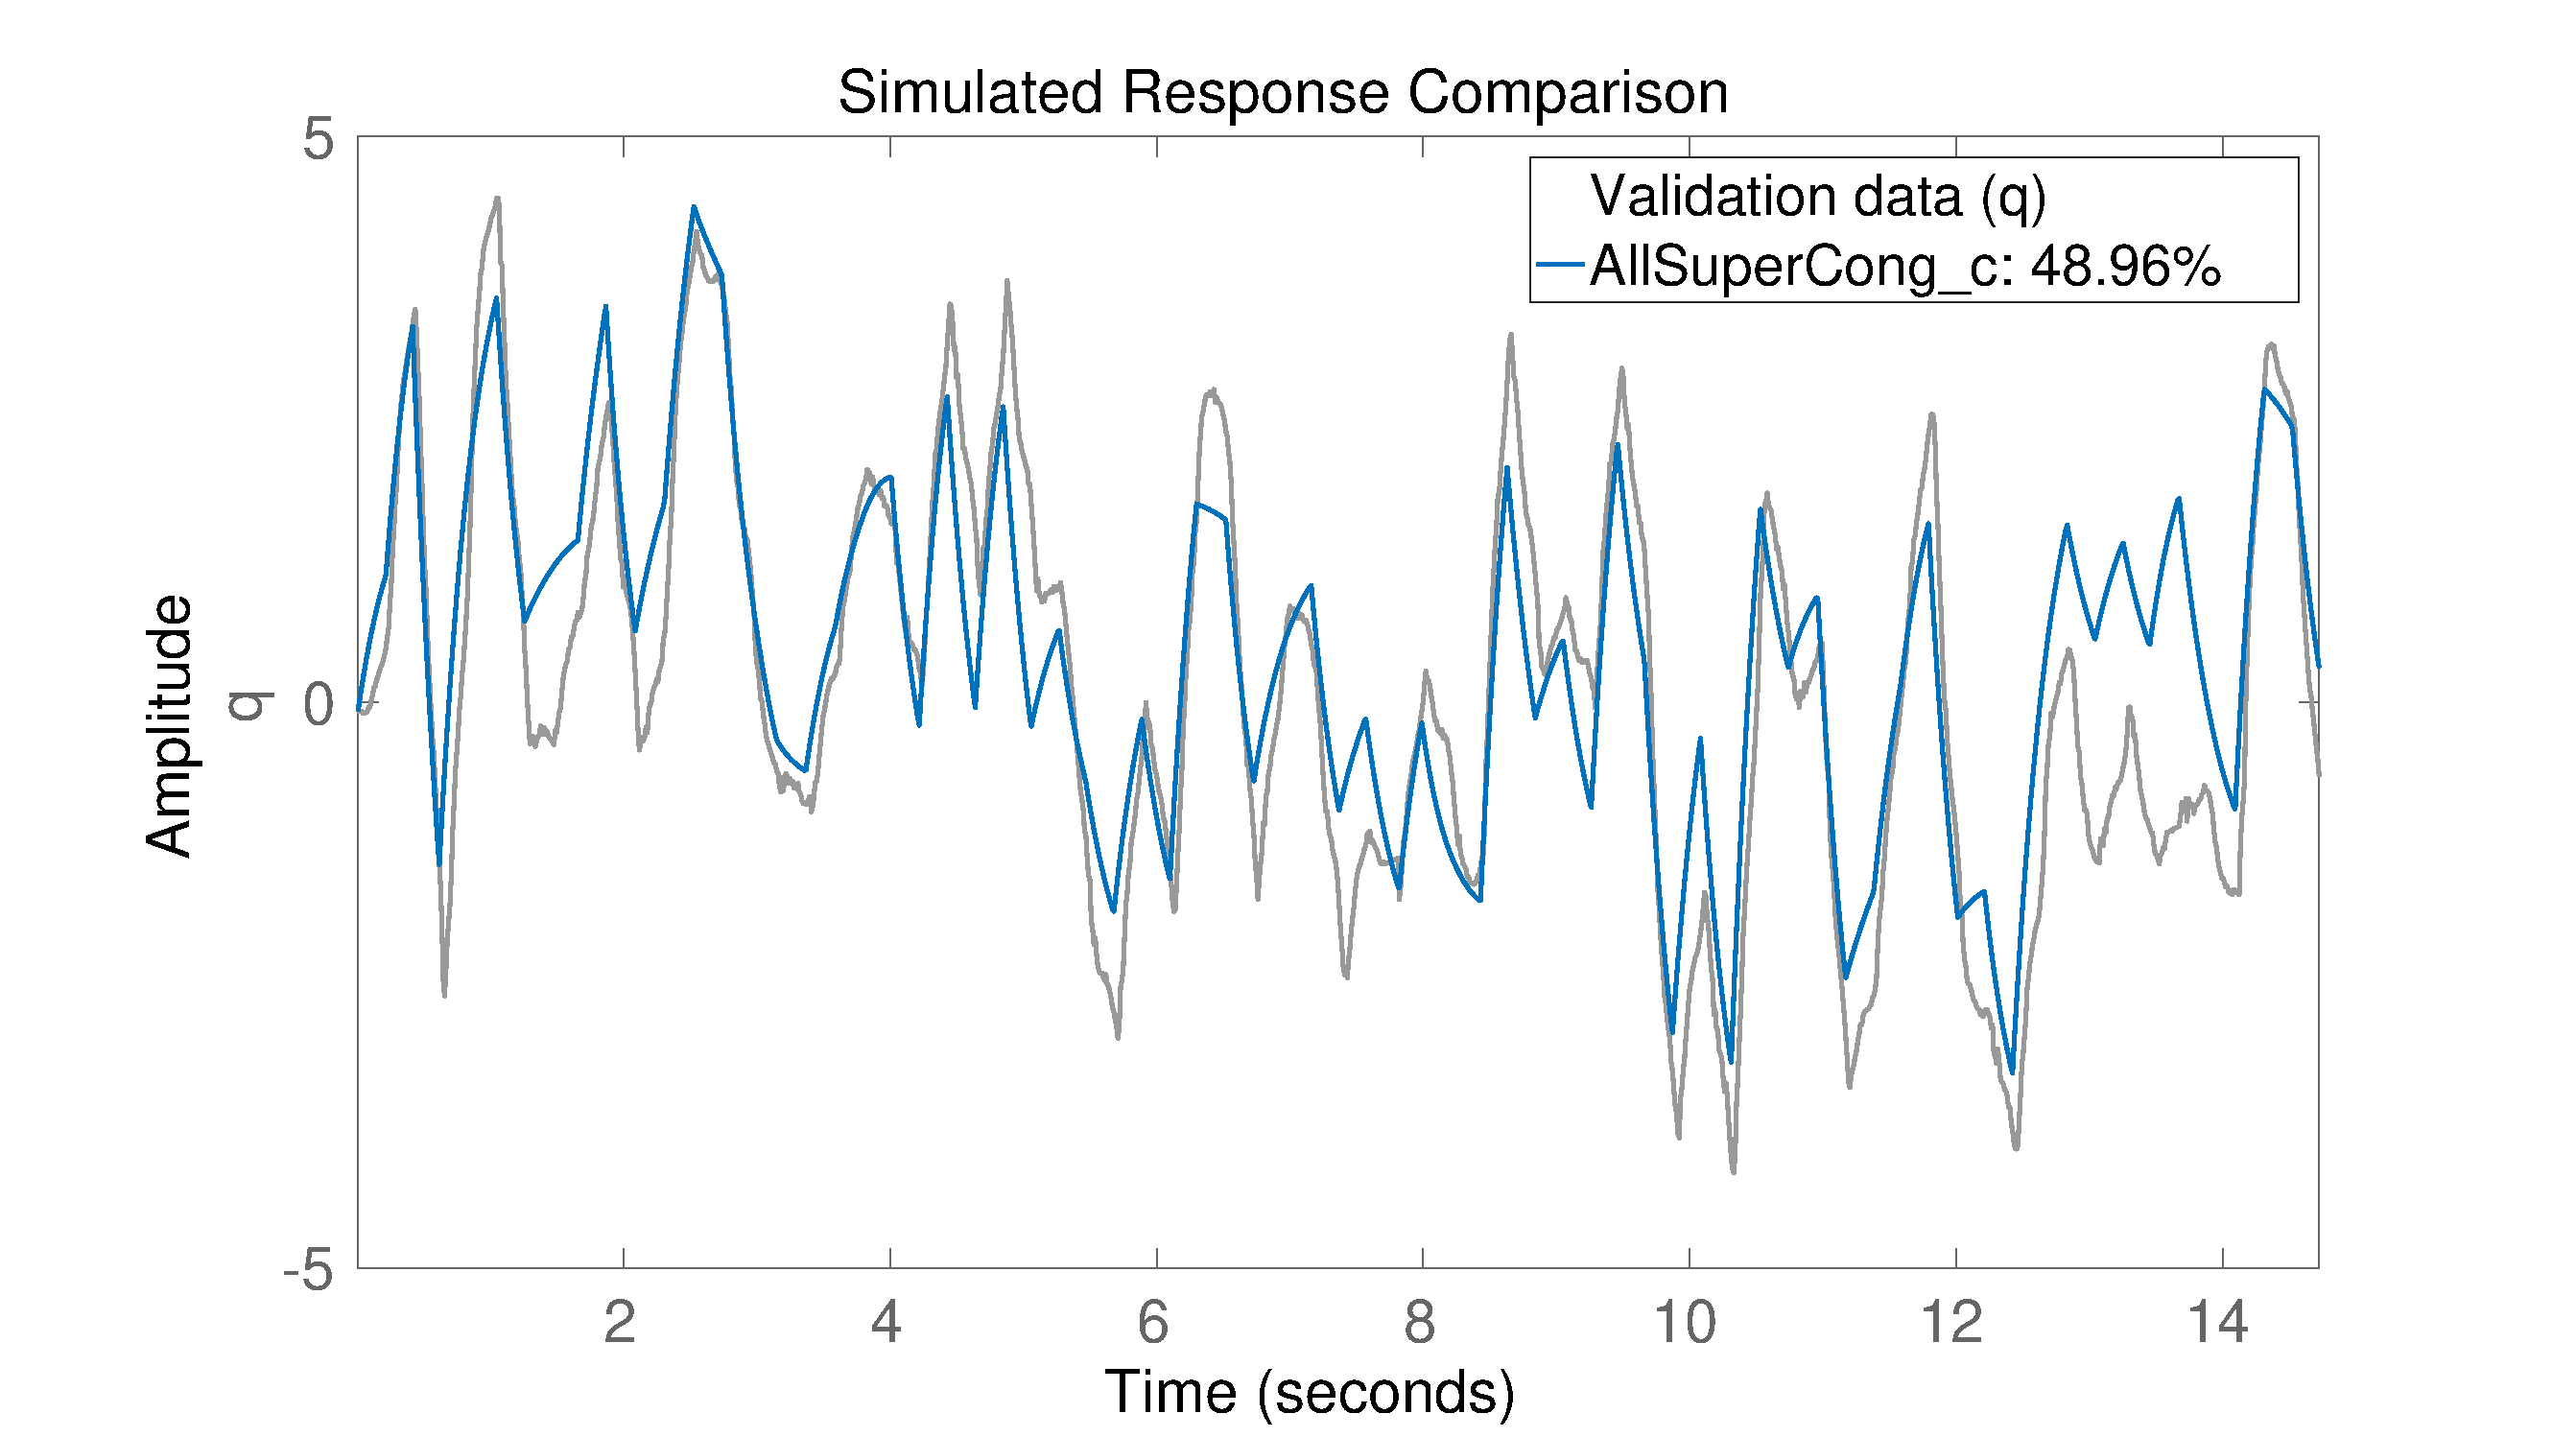
\includegraphics[width=0.4\textwidth]{angVelCompareqlz6}}
  \qquad
  \subfloat[][\label{fig:angVelComparerlz6}Angular velocity around the \abbrROV's z-axis.]{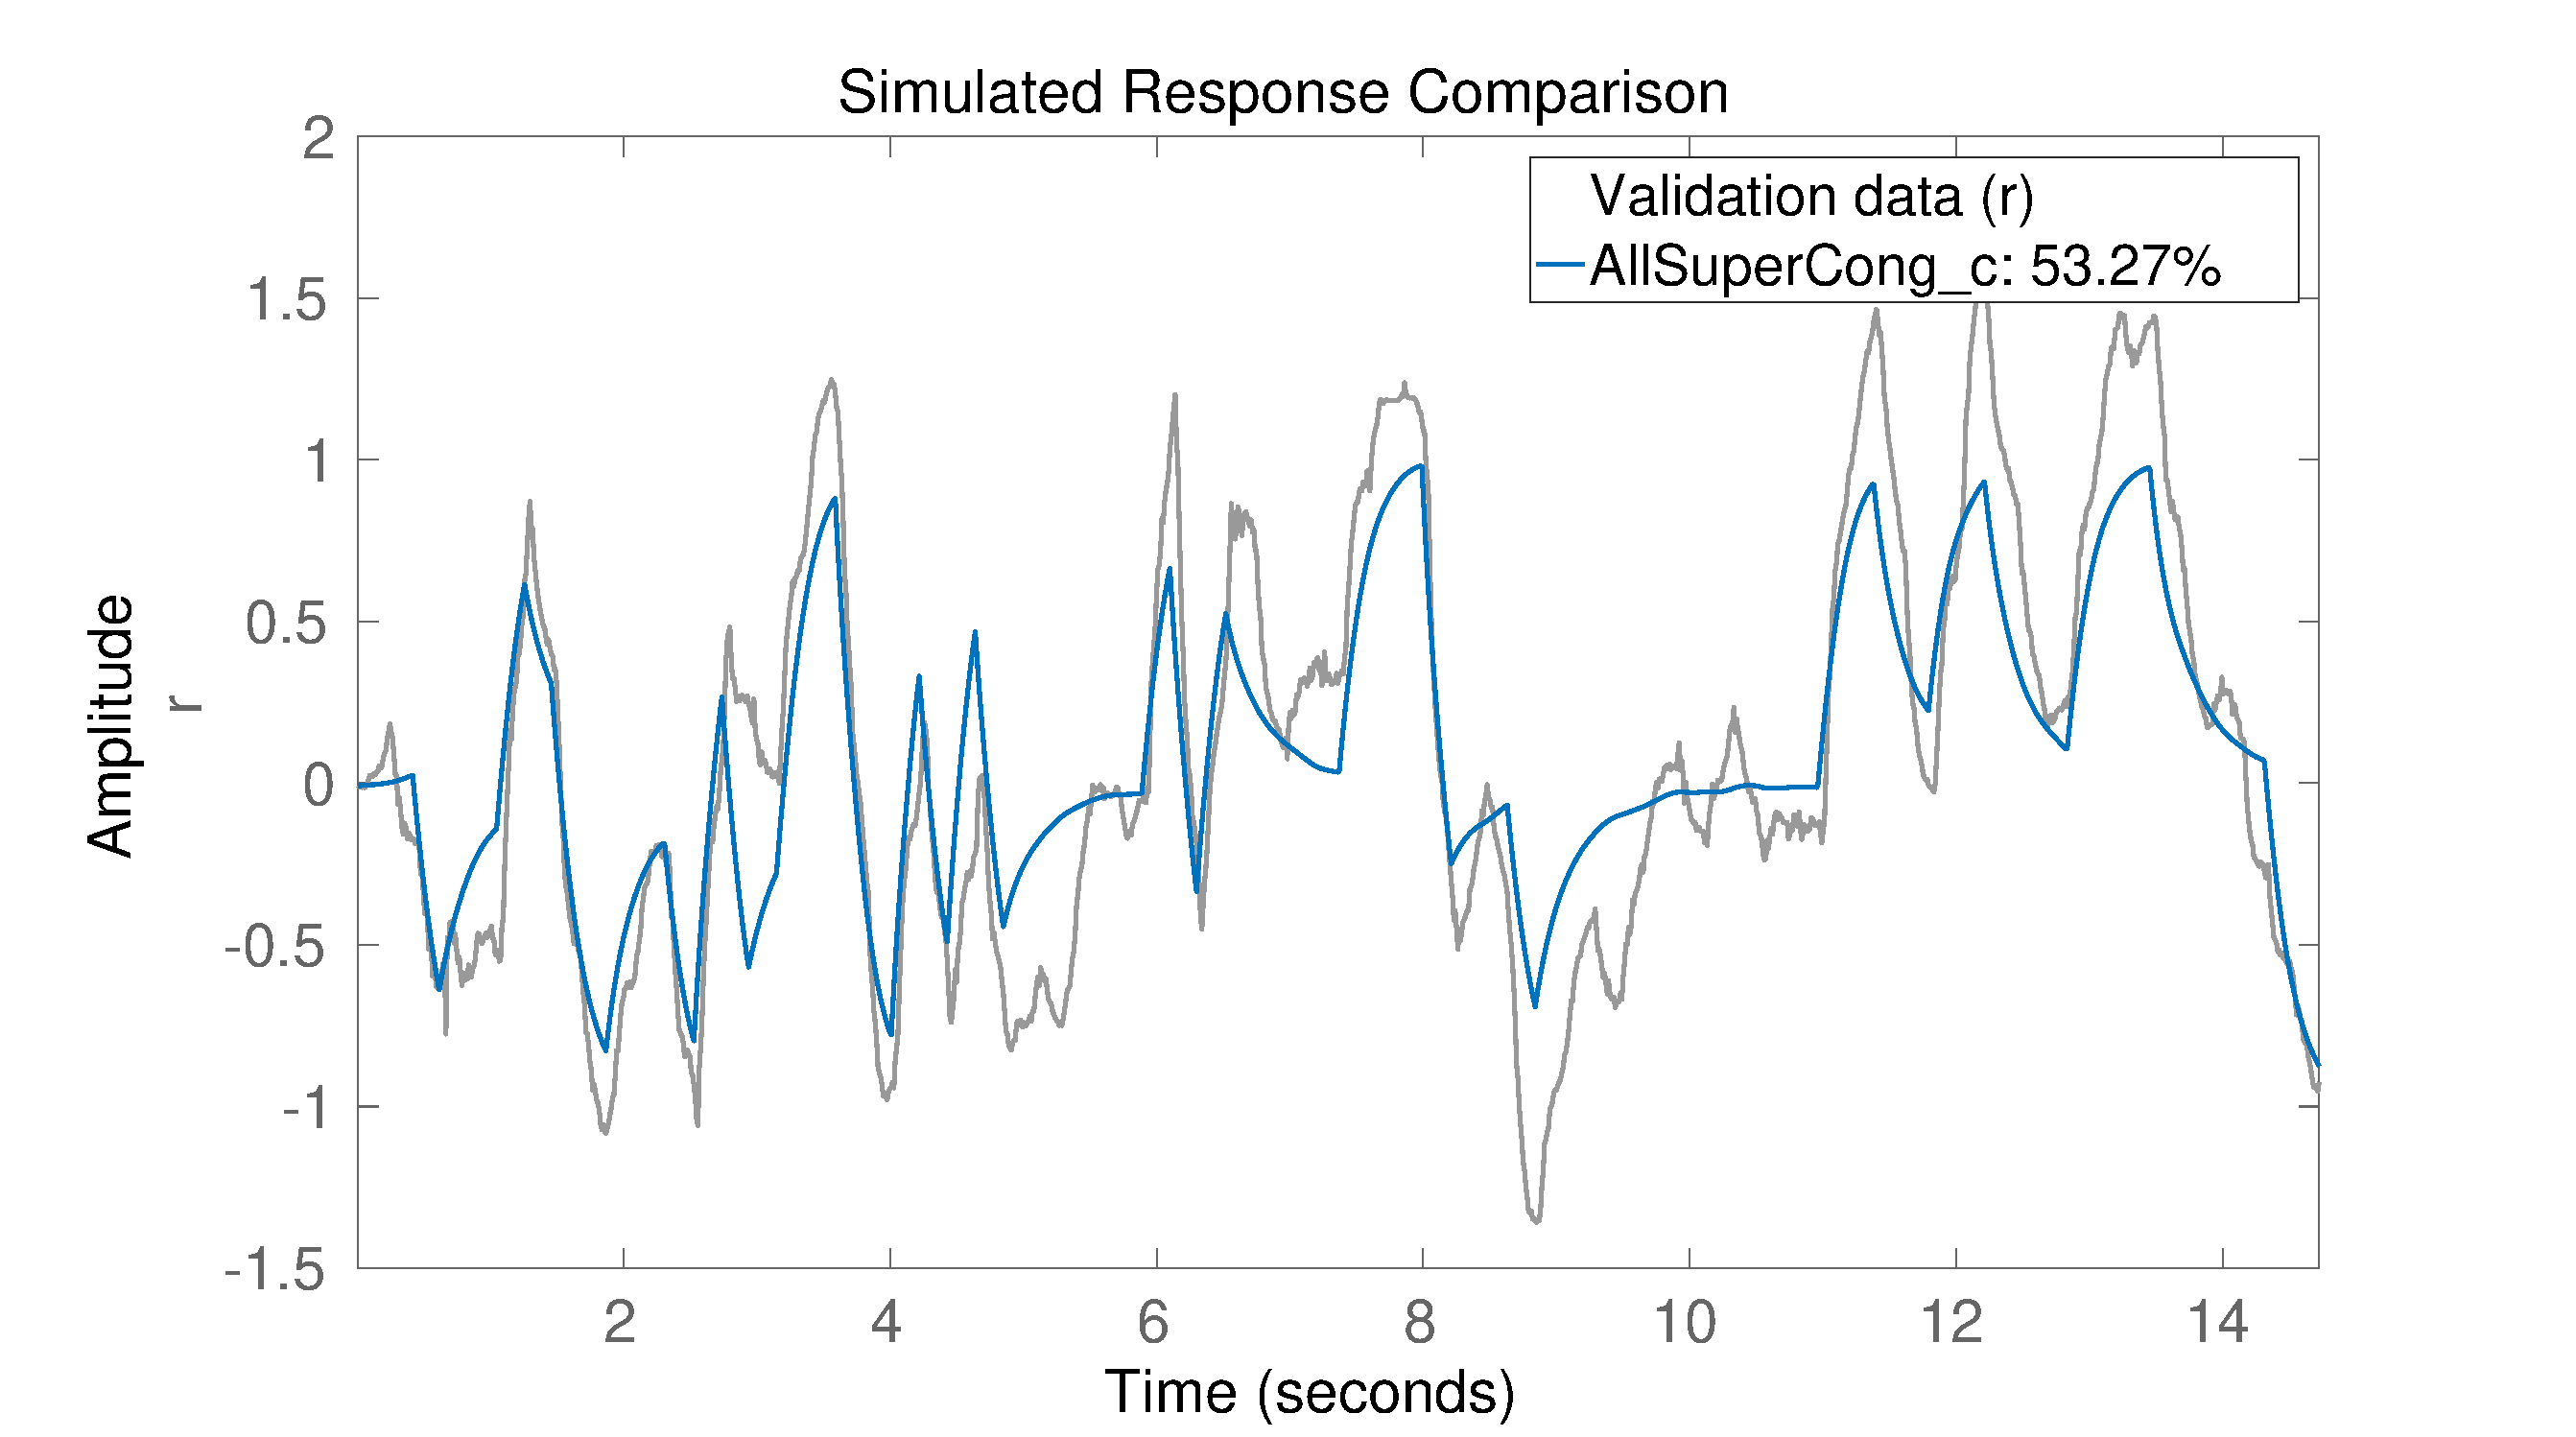
\includegraphics[width=0.4\textwidth]{angVelComparerlz6}}
    \qquad
  \subfloat[][\label{fig:linAccComparexlz6}Linear acceleration in the \abbrROV's x-axis.]{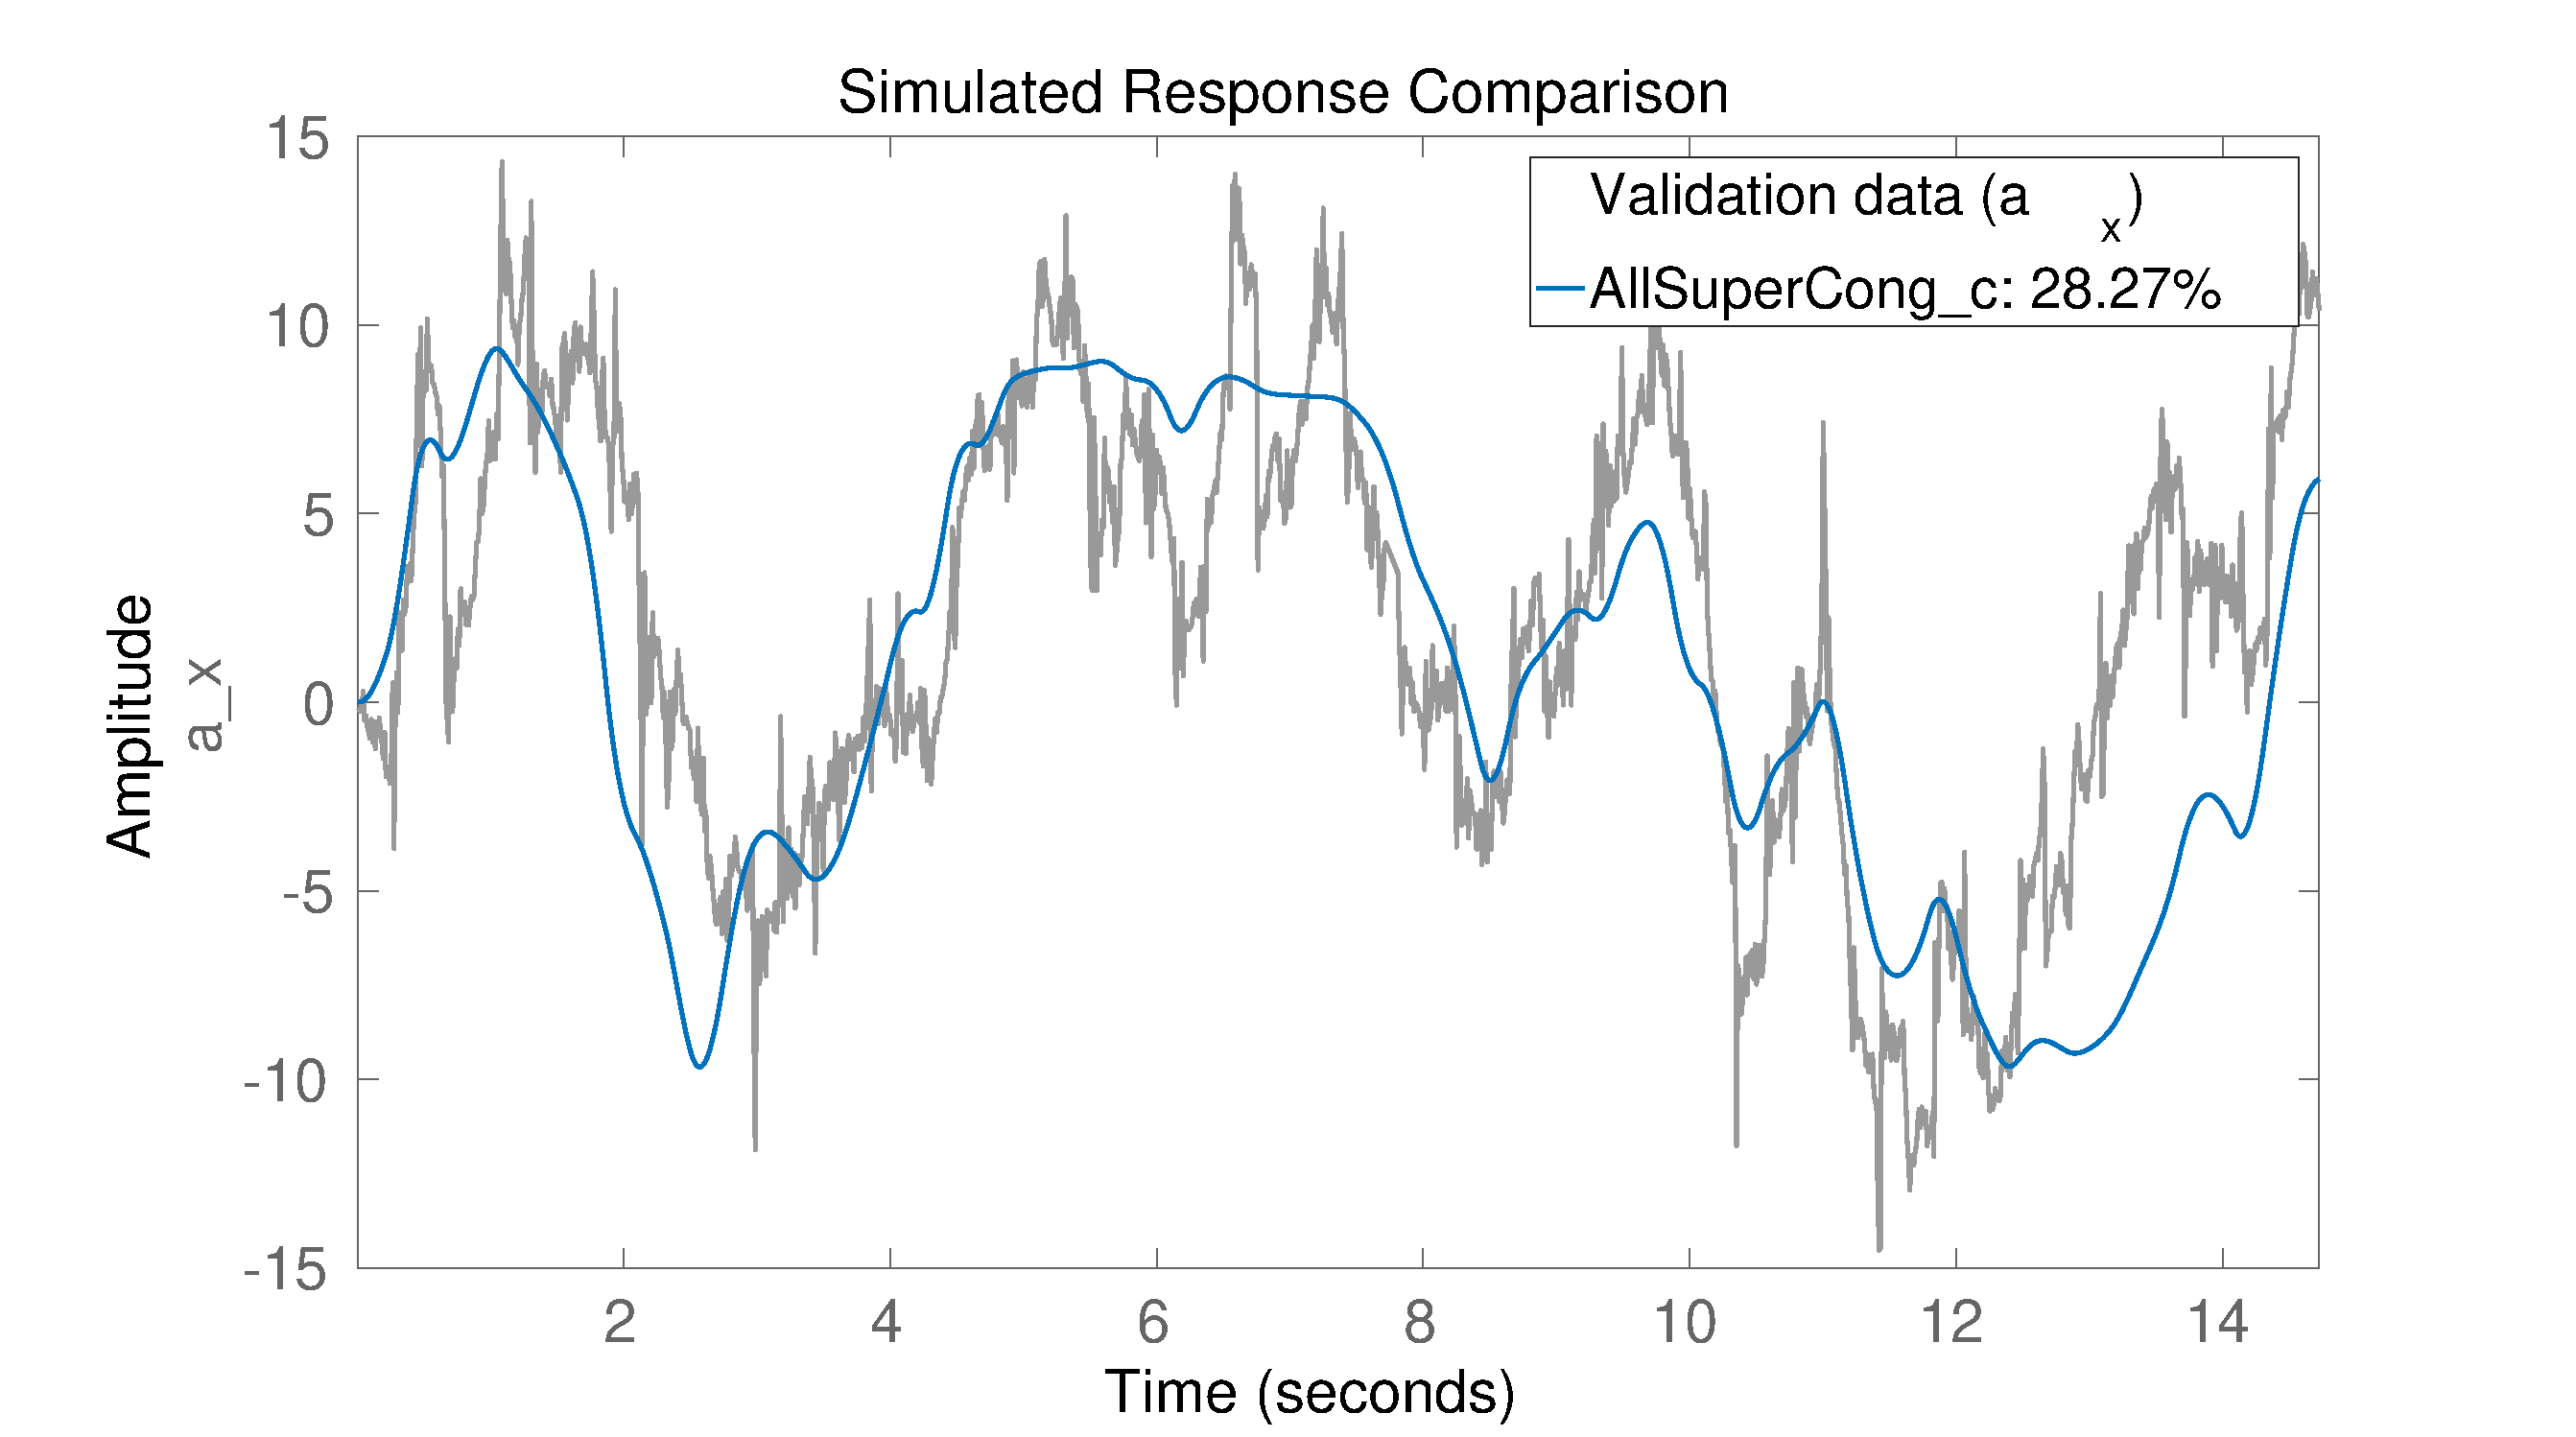
\includegraphics[width=0.4\textwidth]{linAccComparexlz6}}
    \qquad
  \subfloat[][\label{fig:linAccCompareylz6}Linear acceleration in the \abbrROV's y-axis.]{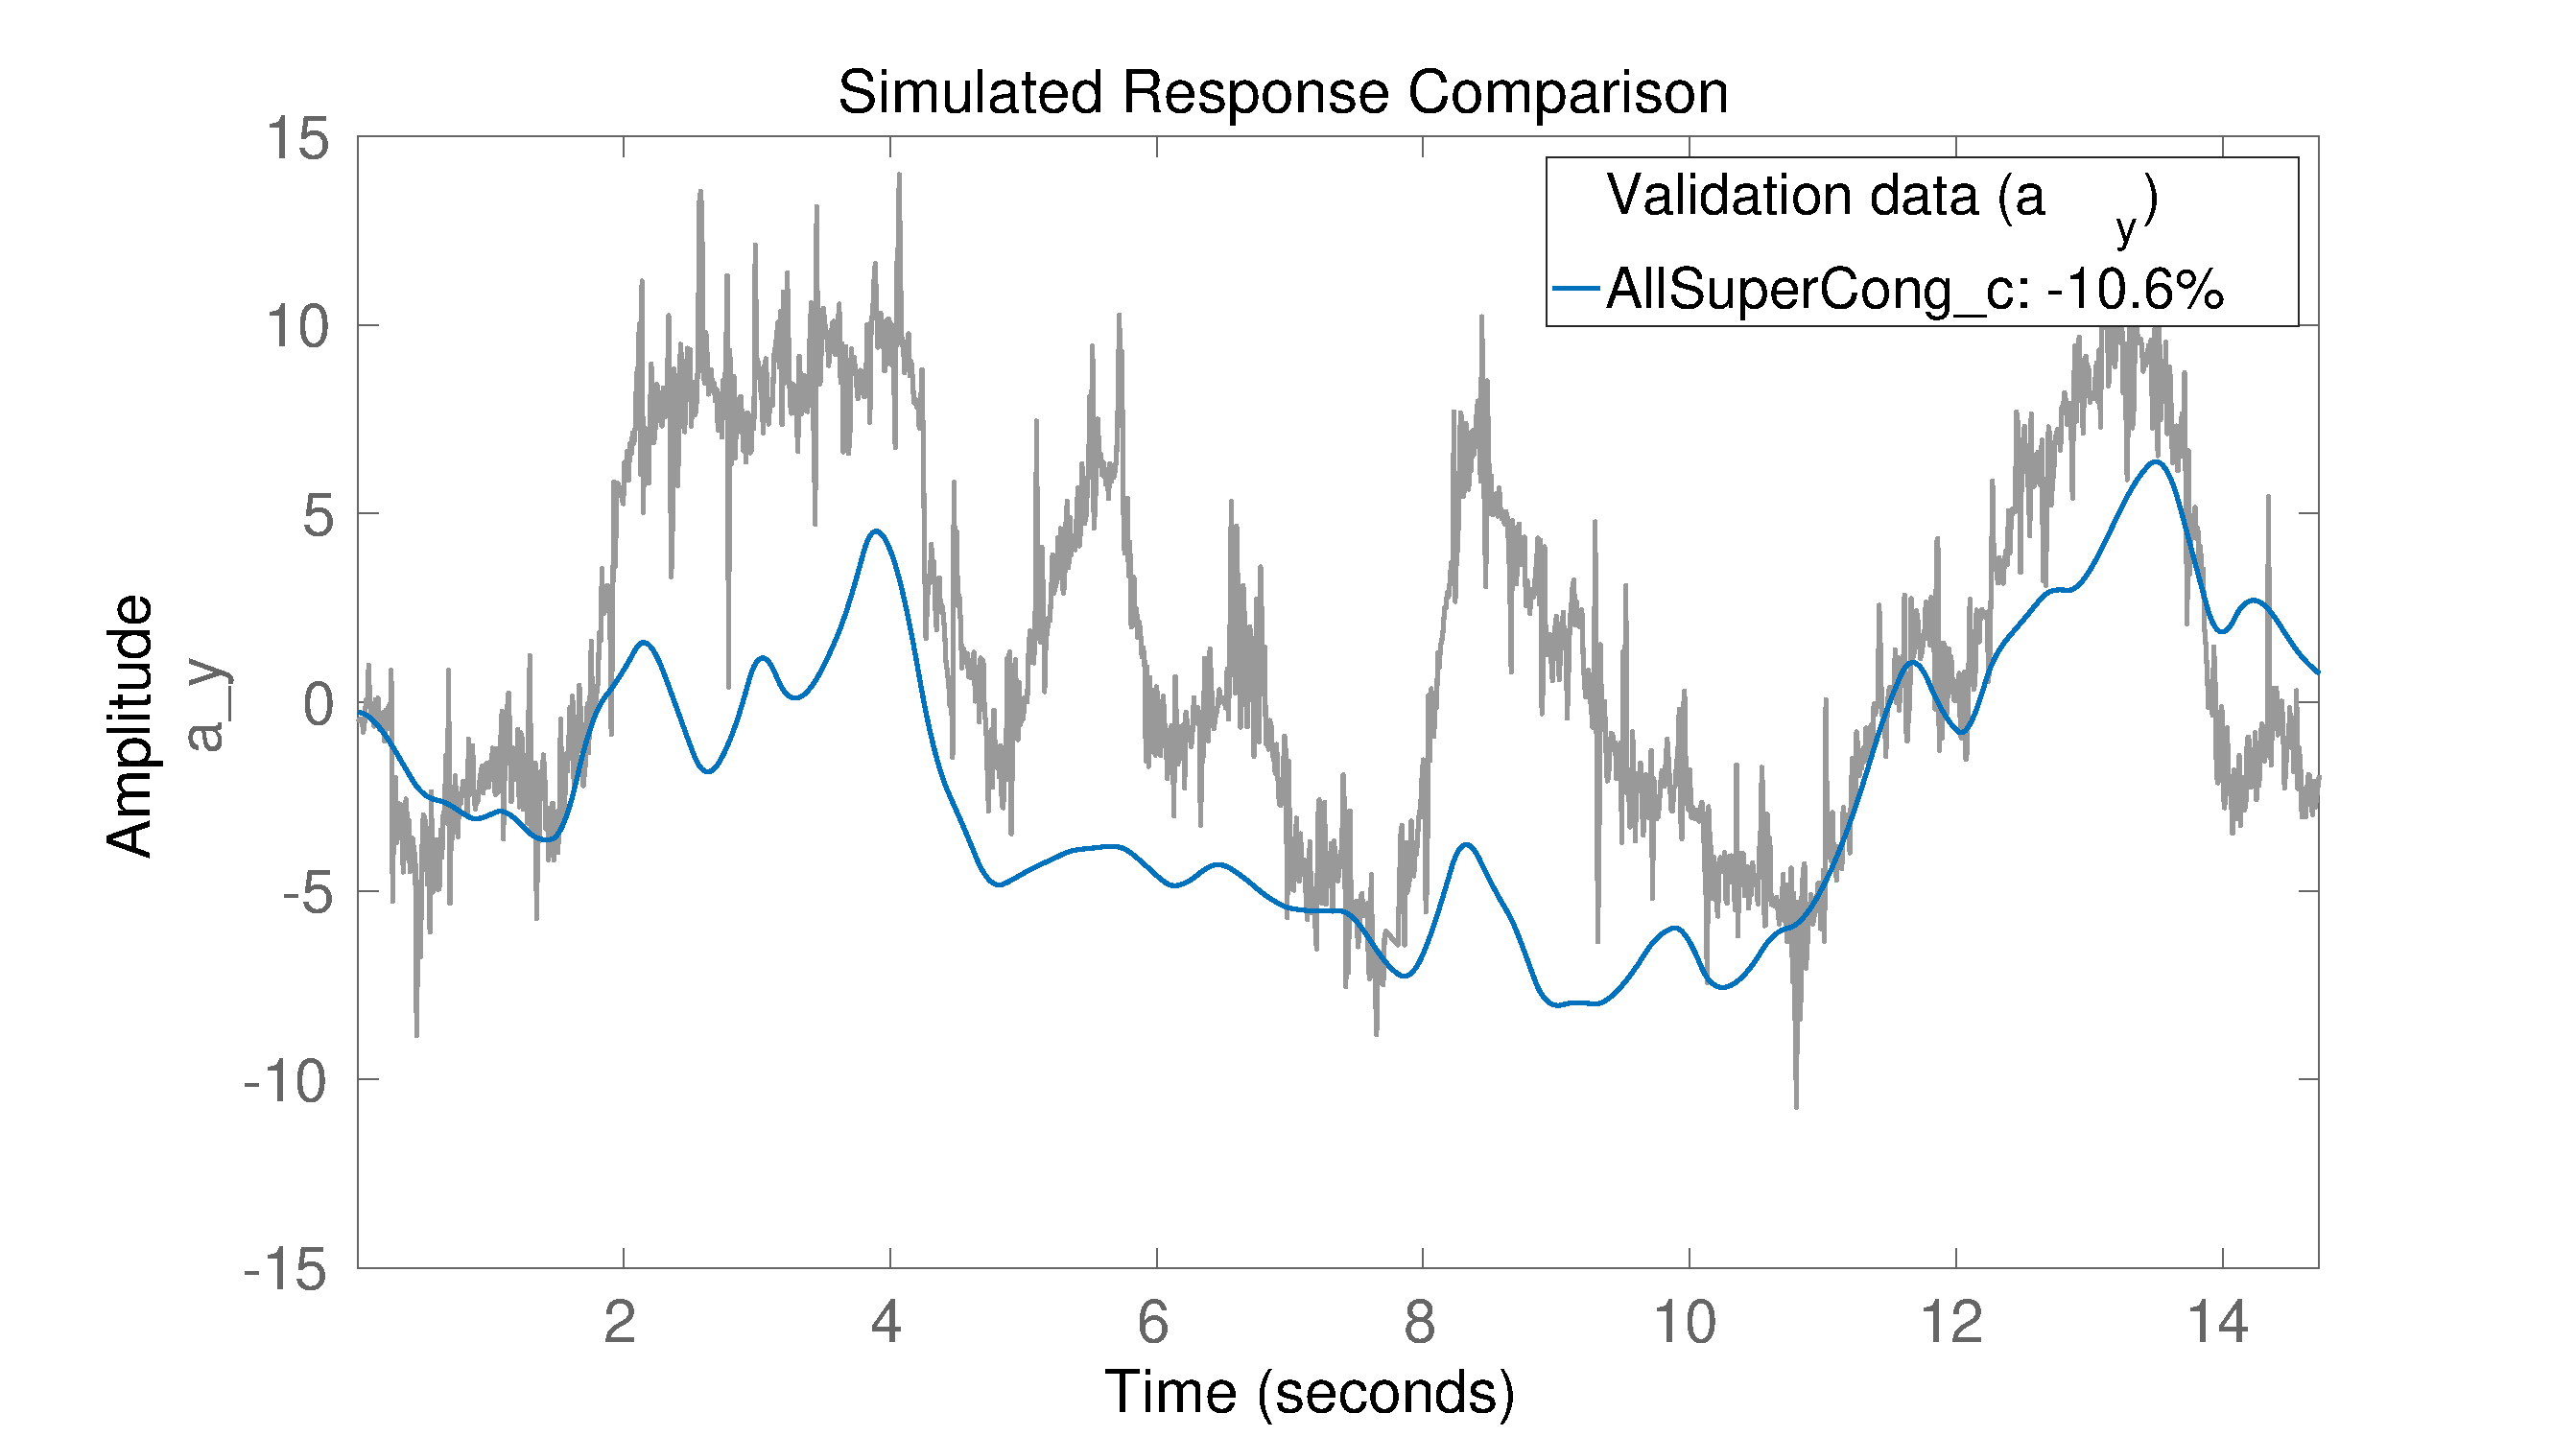
\includegraphics[width=0.4\textwidth]{linAccCompareylz6}}
    \qquad
  \subfloat[][\label{fig:linAccComparezlz6}Linear acceleration in the \abbrROV's z-axis.]{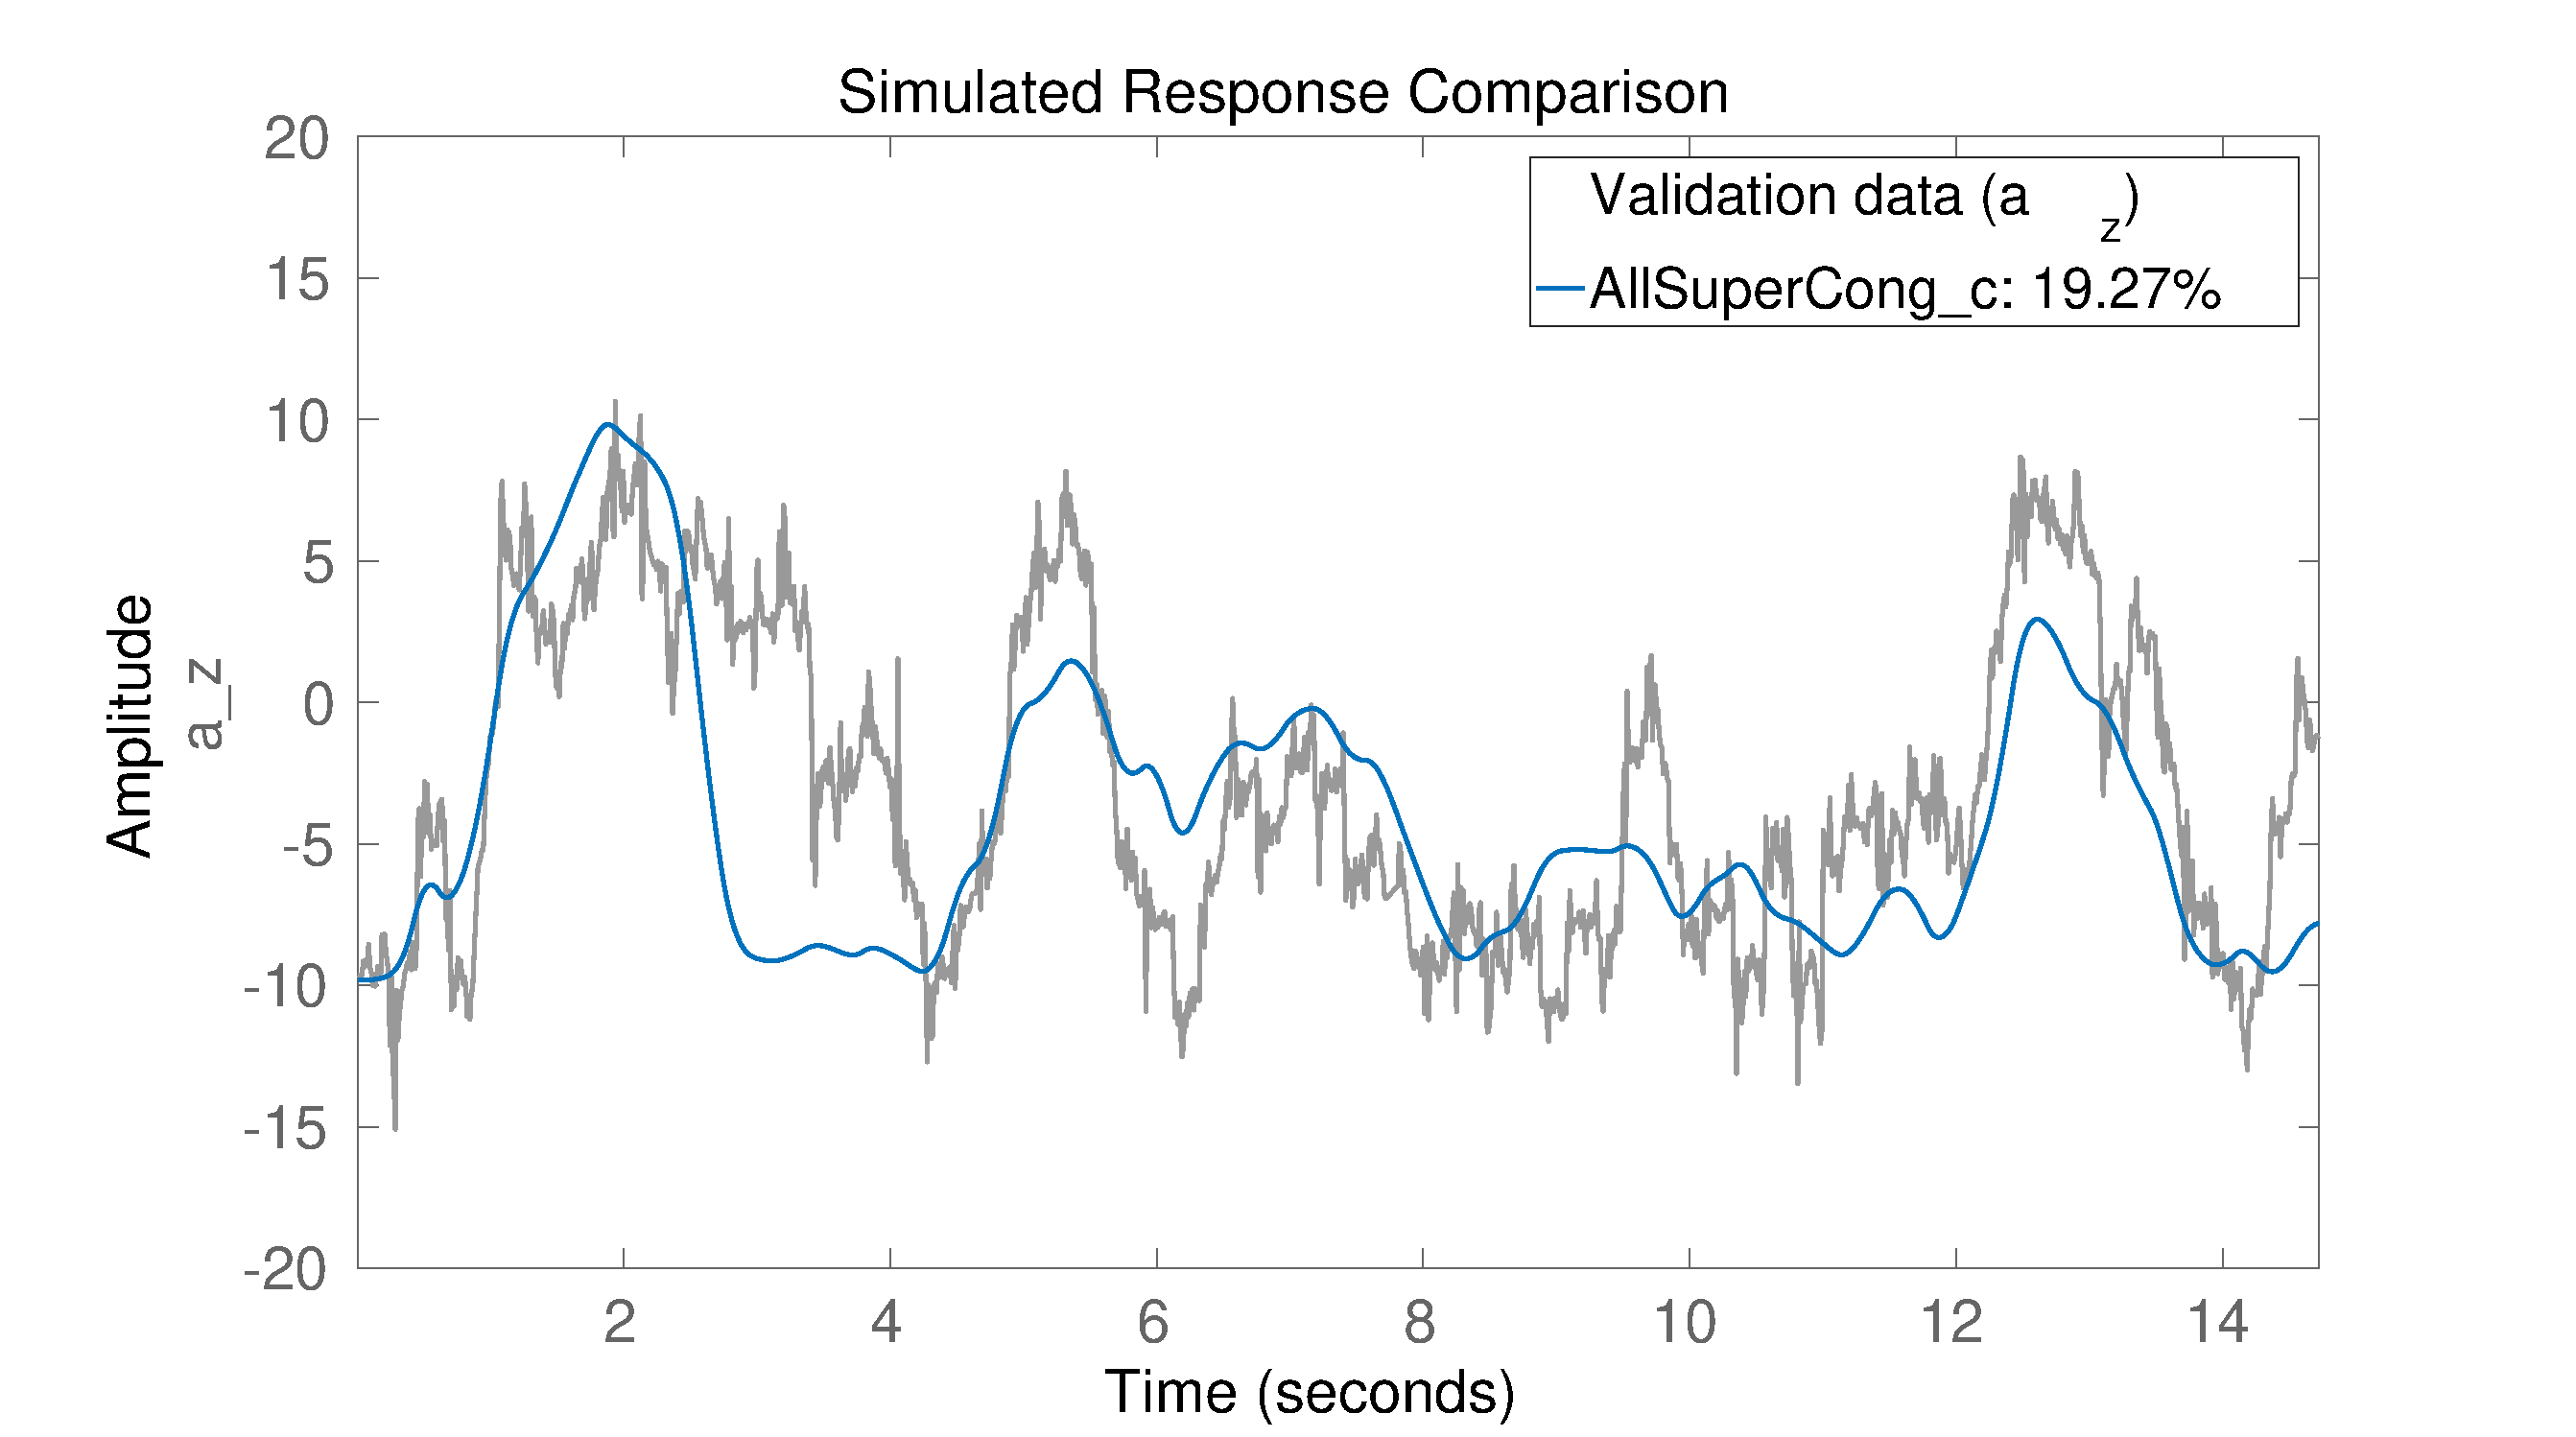
\includegraphics[width=0.4\textwidth]{linAccComparezlz6}}
  \caption{\label{fig:angVelComparelz6}%
    Comparison of validation data (grey) against the simulated response from the model(blue). The fit for the model in each state is stated in each plot. The estimation used angular velocities and linear accelerations as outputs. The model describes $q$ an $r$ well which can be seen in the high fit. The model do not describe the linear accelerations and $p$ well, this can be seen in the low fit.}
\end{figure}

\begin{table}[hbp]
  \centering
  \caption{\label{tab:ResultEstimAngular}%
    The estimated parameters from the prediction-error method using estimated angles as inputs and angular velocities as outputs (left) and the estimated parameters from the prediction-error method using angular velocities and linear acceleration as outputs (right).}
  \begin{tabular}{l p{0.18\linewidth} p{0.18\linewidth} p{0.18\linewidth}}
    \toprule%
    \textbf{Notation}  & \textbf{Starting Value} & \textbf{Estimated Value} & \textbf{Estimated Value}\\
    \otoprule%   
    % Parameters that will be estimated
	$z_B$               & -0.01 	\meter 						& -0.0178 \meter 						& -0.0294  	\meter\\
    $\Kp$               & -1   	\kilogram\usk\meter\squared 	& -1.3275  	\kilogram\usk\meter\squared	& -2.5940 	\kilogram\usk\meter\squared\\
    $\Kpabsp$           & -1  	\kilogram\usk\meter\squared	& 	0  		\kilogram\usk\meter\squared	& -0.3092  	\kilogram\usk\meter\squared\\
    $\Mq$               & -1  	\kilogram\usk\meter\squared	& -1.1925	\kilogram\usk\meter\squared	& -2.0425  	\kilogram\usk\meter\squared\\
    $\Mqabsq$           & -1  	\kilogram\usk\meter\squared	& -0.1094  \kilogram\usk\meter\squared	& -0.0071  	\kilogram\usk\meter\squared\\
    $\Nr$               & -1  	\kilogram\usk\meter\squared	&  -2.7838 	\kilogram\usk\meter\squared	& -2.9364	\kilogram\usk\meter\squared\\
    $\Nrabsr$           & -1  	\kilogram\usk\meter\squared	& -0.6751	\kilogram\usk\meter\squared	& -2.1843 	\kilogram\usk\meter\squared\\
    $A_p$               & 1.5 	\kilogram\usk\meter\squared	& 0.3255  	\kilogram\usk\meter\squared	& 0.7186 	\kilogram\usk\meter\squared\\
    $B_q$               & 1.5 	\kilogram\usk\meter\squared	& 0.3753 	\kilogram\usk\meter\squared	& 0.6112		\kilogram\usk\meter\squared\\
    $C_r$               & 1.5 	\kilogram\usk\meter\squared	& 0.9546 	\kilogram\usk\meter\squared	&  1.0981	\kilogram\usk\meter\squared\\
    \bottomrule%
  \end{tabular}
\end{table}   
%%%%%%%%%%%%%%%%%%%%%%%%%%%%%%%%%
\section{Extended Kalman Filter Estimation}\label{sec:KalmanEstimation}\index{EKF@\abbrEKF!abbreviation} 
To circumvent the issues with estimating the initial state during the prediction-error method, a \abbrEKF was used to estimated the parameters. An \abbrEKF can  be used to estimate parameters by extending the state vector of the \abbrEKF with the parameters that need to be estimated \citep{Roger}.  \index{Model structure}
\begin{equation}
\bar{\boldsymbol{x}} = \begin{bmatrix}
\boldsymbol{x}_k\\
\boldsymbol{\theta}_k
\end{bmatrix}
\end{equation}
The added parameters were modelled using constant position, which gave the following augmented state-space form 
\begin{equation}
\bar{\boldsymbol{x}}_{k+1}(\boldsymbol{\theta}) =\begin{bmatrix}
\boldsymbol{f}(\boldsymbol{x}_k(\boldsymbol{\theta}),\boldsymbol{u}_k,\boldsymbol{\theta})\\
\boldsymbol{\theta}_k
\end{bmatrix} 
+\boldsymbol{v}
\end{equation}
\begin{equation}
\boldsymbol{y}_k=\boldsymbol{h}(\bar{\boldsymbol{x}}_k(\boldsymbol{\theta}),\boldsymbol{u}_k)
\end{equation}
Since the \abbrEKF tries to minimise state variance it will also try to estimate the parameters $\boldsymbol{\theta}$ if they are included in the state vector \citep{Roger}.

%\subsection{Implementation}\label{sec:KalmanEstimatorImpl}
%The reparametrised model \eqref{eq:quatModel} was used to model $\etaVector$ and $\nuVector$. Measurement equations were taken from \Chapterref{cha:sensor_fusion}. Each model parameter was modelled as a state using a constant position motion model and the motion model was discretised using the Euler forward discretisation method. The complete discrete model is
%\begin{equation}
%\label{eq:motionModelKalman}
%\begin{bmatrix}
%\etaVector_{k+1}\\ 
%\nuVector_{k+1}\\
%\boldsymbol{b}_{k+1}\\
%\boldsymbol{\theta}_{k+1}
%\end{bmatrix} = 
%\begin{bmatrix}
%\etaVector_k + T_s \boldsymbol{T}(\etaVector_k)\nuVector_k\\
%\nuVector_k + T_s f(\etaVector_k,\nuVector_k,\boldsymbol{\theta}_k)\\
%\boldsymbol{b}_k\\
%\boldsymbol{\theta}_k
%\end{bmatrix}
%+ \begin{bmatrix}
%\boldsymbol{v}_{\etaVector}\\
%\boldsymbol{v}_{\nuVector}\\
%\boldsymbol{v}_{\boldsymbol{b}}\\
%\boldsymbol{v}_{\boldsymbol{\theta}}
%\end{bmatrix}
%\end{equation}
%Here, $\boldsymbol{\theta}$ is a vector containing the parameters that were estimated. The vector-valued function $\boldsymbol{f}(\etaVector,\nuVector,\boldsymbol{\theta})$ is \eqref{eq:quatModel}. The vector $\boldsymbol{b}$  contains the biases of the gyroscope. The vector $\boldsymbol{v}$ is the system noise and is assumed to enter each term directly, this resulted in a diagonal $\boldsymbol{Q}$-matrix when implementing the model in the \abbrEKF. The matrix $\boldsymbol{T}(\etaVector)$ is an angular velocity transformation matrix using the quaternion form of $\etaVector$ and is defined in \Chapterref{cha:modelling}. Measurement equations are taken from \sectionref{sec:Meas}.

To increase the performance of the filter a method for outlier detection and rejection was implemented. Since time updates were done batch wise it was decided to use a different form of outlier rejection and not to reimplement the method used in \sectionref{sec:Meas}. The outlier rejection method is based on the assumption that the normalised innovation \begin{equation} \label{eq:chi}
\boldsymbol{\epsilon}^T \boldsymbol{S}^{-1} \boldsymbol{\epsilon} \sim \chi_{n}^{2}
\end{equation}
where $n$ is the number of measurements. To check the validity of a single measurement, \eqref{eq:chi} gives that $\epsilon_i^{2}/S_{i,i} \sim \chi_{1}^{2}$ \citep{sensorfusion}. This is implemented in the \abbrEKF using \Algoref{alg:outlier}.
\begin{algorithm}[h]
\caption{The outlier rejection algorithm used during the measurement update step of the parameter estimation \abbrEKF.}\label{alg:outlier}
\textbf{1.} Calculate $\boldsymbol{S}=h_{\boldsymbol{x}} \boldsymbol{P} h_{\boldsymbol{x}}^T + \boldsymbol{R}$ and the innovation $\epsilon$.
\\
\textbf{2.} For each row $i$ in $\boldsymbol{\epsilon}$ do the comparison
\begin{equation}
\epsilon_{i}^{2} > \sigma_i S_{i,i}
\end{equation}
If the expression holds true, remove the $i$:th row from $\boldsymbol{\epsilon}$ and the $i$:th row and column from $\boldsymbol{S}$ and $h_{\boldsymbol{x}}$.\\
\textbf{3.} Proceed with the Kalman algorithm using the cropped $h_{\boldsymbol{x}}$, $\boldsymbol{S}$ and $\boldsymbol{\epsilon}$.

Here, $\boldsymbol{\sigma}$ is a $n\times1$ dimensional design variable and $n$ is the number of measurements that are used in the \abbrEKF. A higher value of $\sigma_i$ decreases the sensitivity of the outlier rejection for the $i$:th measurement.
\end{algorithm}

%The filter was run on each collected dataset. The final values of $\hat{\boldsymbol{\theta}}$ from a dataset were used as initial values for $\hat{\boldsymbol{\theta}}$ when the filter was applied on the next dataset. The same was done for the covariance matrix $\boldsymbol{P}$. The final covariance from an earlier run was set as the initial covariance when the filter was applied on subsequent dataset. At completion the parameters were entered in a simulator which was feed with the control signals from the corresponding dataset. The simulated  output was then compared with the original data.

\section{Estimation Using an Extended Kalman Filter}
The \abbrEKF estimation used the method described in \sectionref{sec:KalmanEstimation} with the model \eqref{eq:quatModel} and quaternions as attitude representation. The estimation was feed with process noise covariance matrix
\begin{equation*}
\boldsymbol{Q}=\text{diag}[\underbrace{\overbrace{1000}^{\times4}}_{\etaVector}... \underbrace{\overbrace{1000}^{\times3}}_{\nuVector}...\underbrace{\overbrace{0.01}^{\times3}}_{\boldsymbol{b}}... \underbrace{\overbrace{0.001}^{\times10}}_{\boldsymbol{\theta}}]\text{ ,}
\end{equation*}
measurement noise covariance matrix
\begin{equation*}
\boldsymbol{R} = \text{diag}[\underbrace{\overbrace{0.001}^{\times3}}_{\text{Gyro}}... \underbrace{\overbrace{0.1}^{\times3}}_{\text{Acc}}... \underbrace{\overbrace{1000}^{\times3}}_{\text{mag}}]
\end{equation*}
Five data sets were feed in to the estimator, while the fourth and fifth were used as validation data. All data sets were of excitations in $p$, $q$ and $r$ simultaneously. Parameter values from the estimation can be viewed together with the initial states in \tableref{tab:ResultKalmanFixedMomentArms}.
\begin{table}[hbp]
  \centering
  \caption{\label{tab:ResultKalmanFixedMomentArms}%
    The estimated parameters from the Kalman estimator method. Moment arms are fixed to measured values.}
  \begin{tabular}{l l p{0.25\linewidth}}
    \toprule%
    \textbf{Notation}  & \textbf{Starting Value} & \textbf{Estimated Value} \\
    \otoprule%   
    % Parameters that will be estimated
    $\etaVector$			&$[1\ 0\ 0\ 0]^T$					&\\
    $\nuVector$			&$[0\ 0\ 0]^T$						&\\
    $\boldsymbol{b}$		&$[0\ 0\ 0]^T$						&\\
	$z_B$               & -0.05 	\meter 						& -0.0463  	\meter\\
    $\Kp$               & -1   	\kilogram\usk\meter\squared 	& -0.9163		\kilogram\usk\meter\squared\\
    $\Kpabsp$           & -1  	\kilogram\usk\meter\squared	& -0.7591  		\kilogram\usk\meter\squared\\
    $\Mq$               & -1  	\kilogram\usk\meter\squared	& -0.8557  		\kilogram\usk\meter\squared\\
    $\Mqabsq$           & -1  	\kilogram\usk\meter\squared	& -0.3396  	\kilogram\usk\meter\squared\\
    $\Nr$               & -1  	\kilogram\usk\meter\squared	& -1.0266		\kilogram\usk\meter\squared\\
    $\Nrabsr$           & -1  	\kilogram\usk\meter\squared	& -1.0236 		\kilogram\usk\meter\squared\\
    $A_p$               & 1 	\kilogram\usk\meter\squared	&  1.0924 		\kilogram\usk\meter\squared\\
    $B_q$               & 1 	\kilogram\usk\meter\squared	&  0.8162		\kilogram\usk\meter\squared\\
    $C_r$               & 1 	\kilogram\usk\meter\squared	&  1.1519		\kilogram\usk\meter\squared\\
    \bottomrule%
  \end{tabular}
\end{table}
The fit of the model using the estimated parameters can be viewed in \figureref{fig:ResultKalmanFixedMomentArms}. The high fit in $q$ and $r$ indicate that the model describes the data well. However, the model does not describe the validation data well in $q$.\index{Fit}
% results kalman fixed moment arms
\begin{figure}[tbp]
  \centering
  \subfloat[][Comparison between a simulated model response and validation data in $p$.]{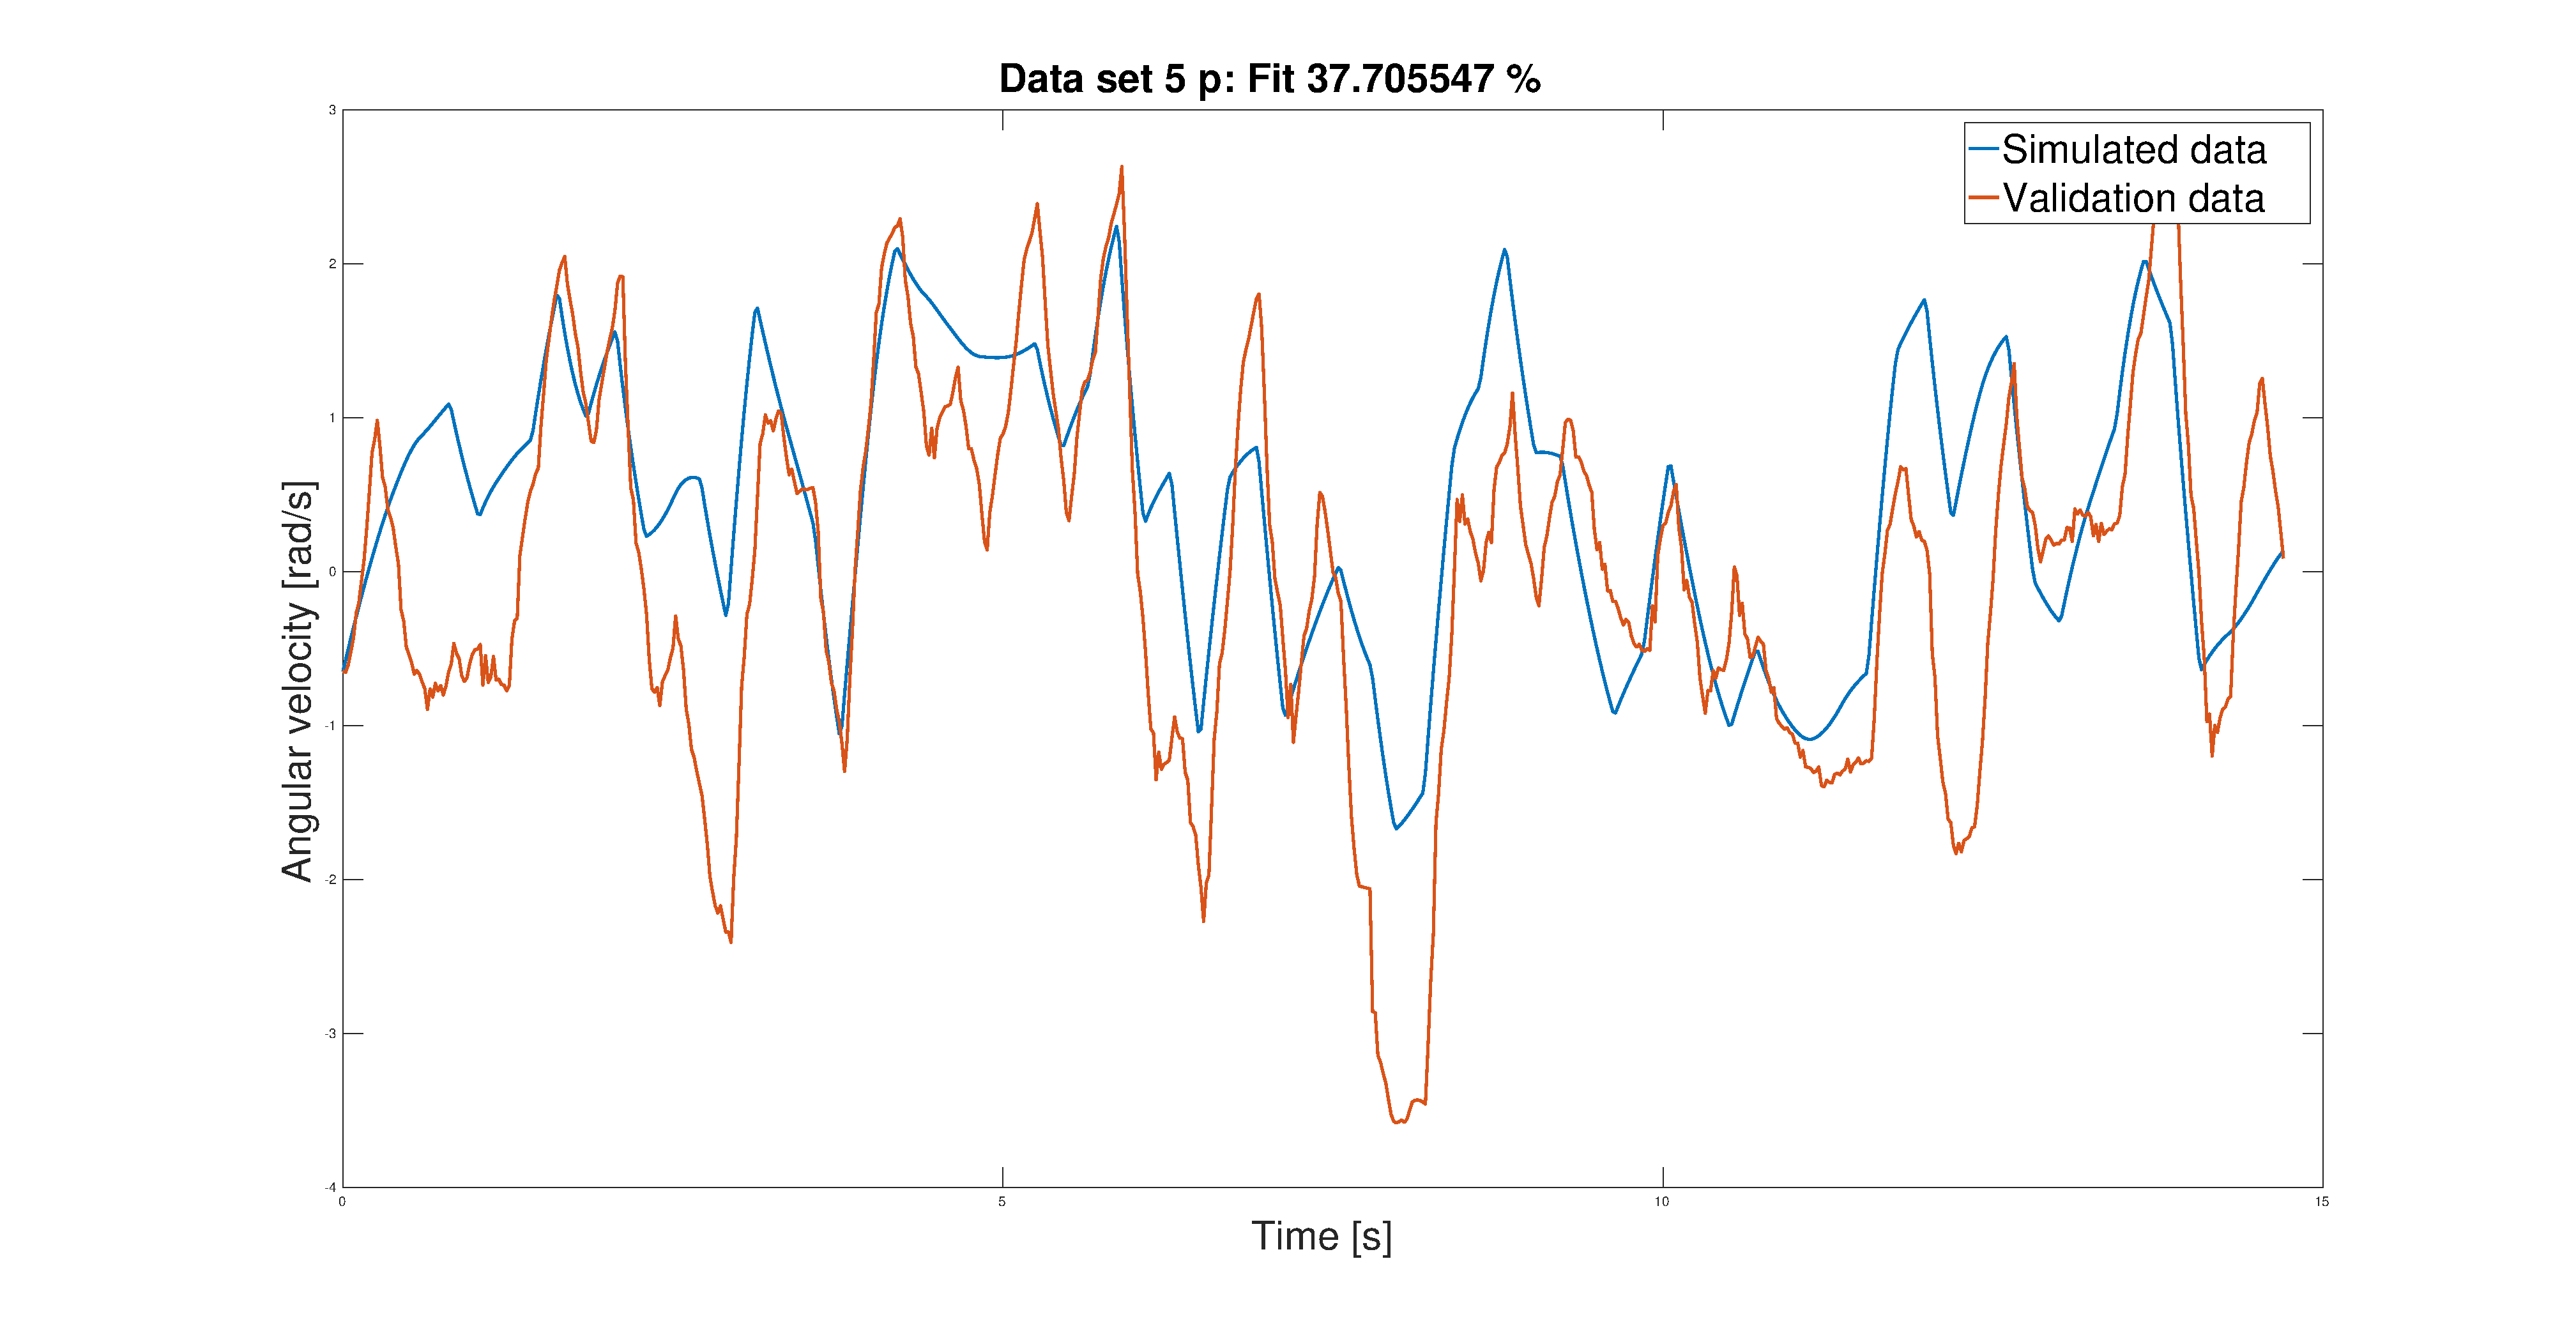
\includegraphics[width=0.7\textwidth]{ResultKalmanFixedMomentP}}
  \qquad
  \subfloat[][Comparison between a simulated model response and validation data in $q$.]{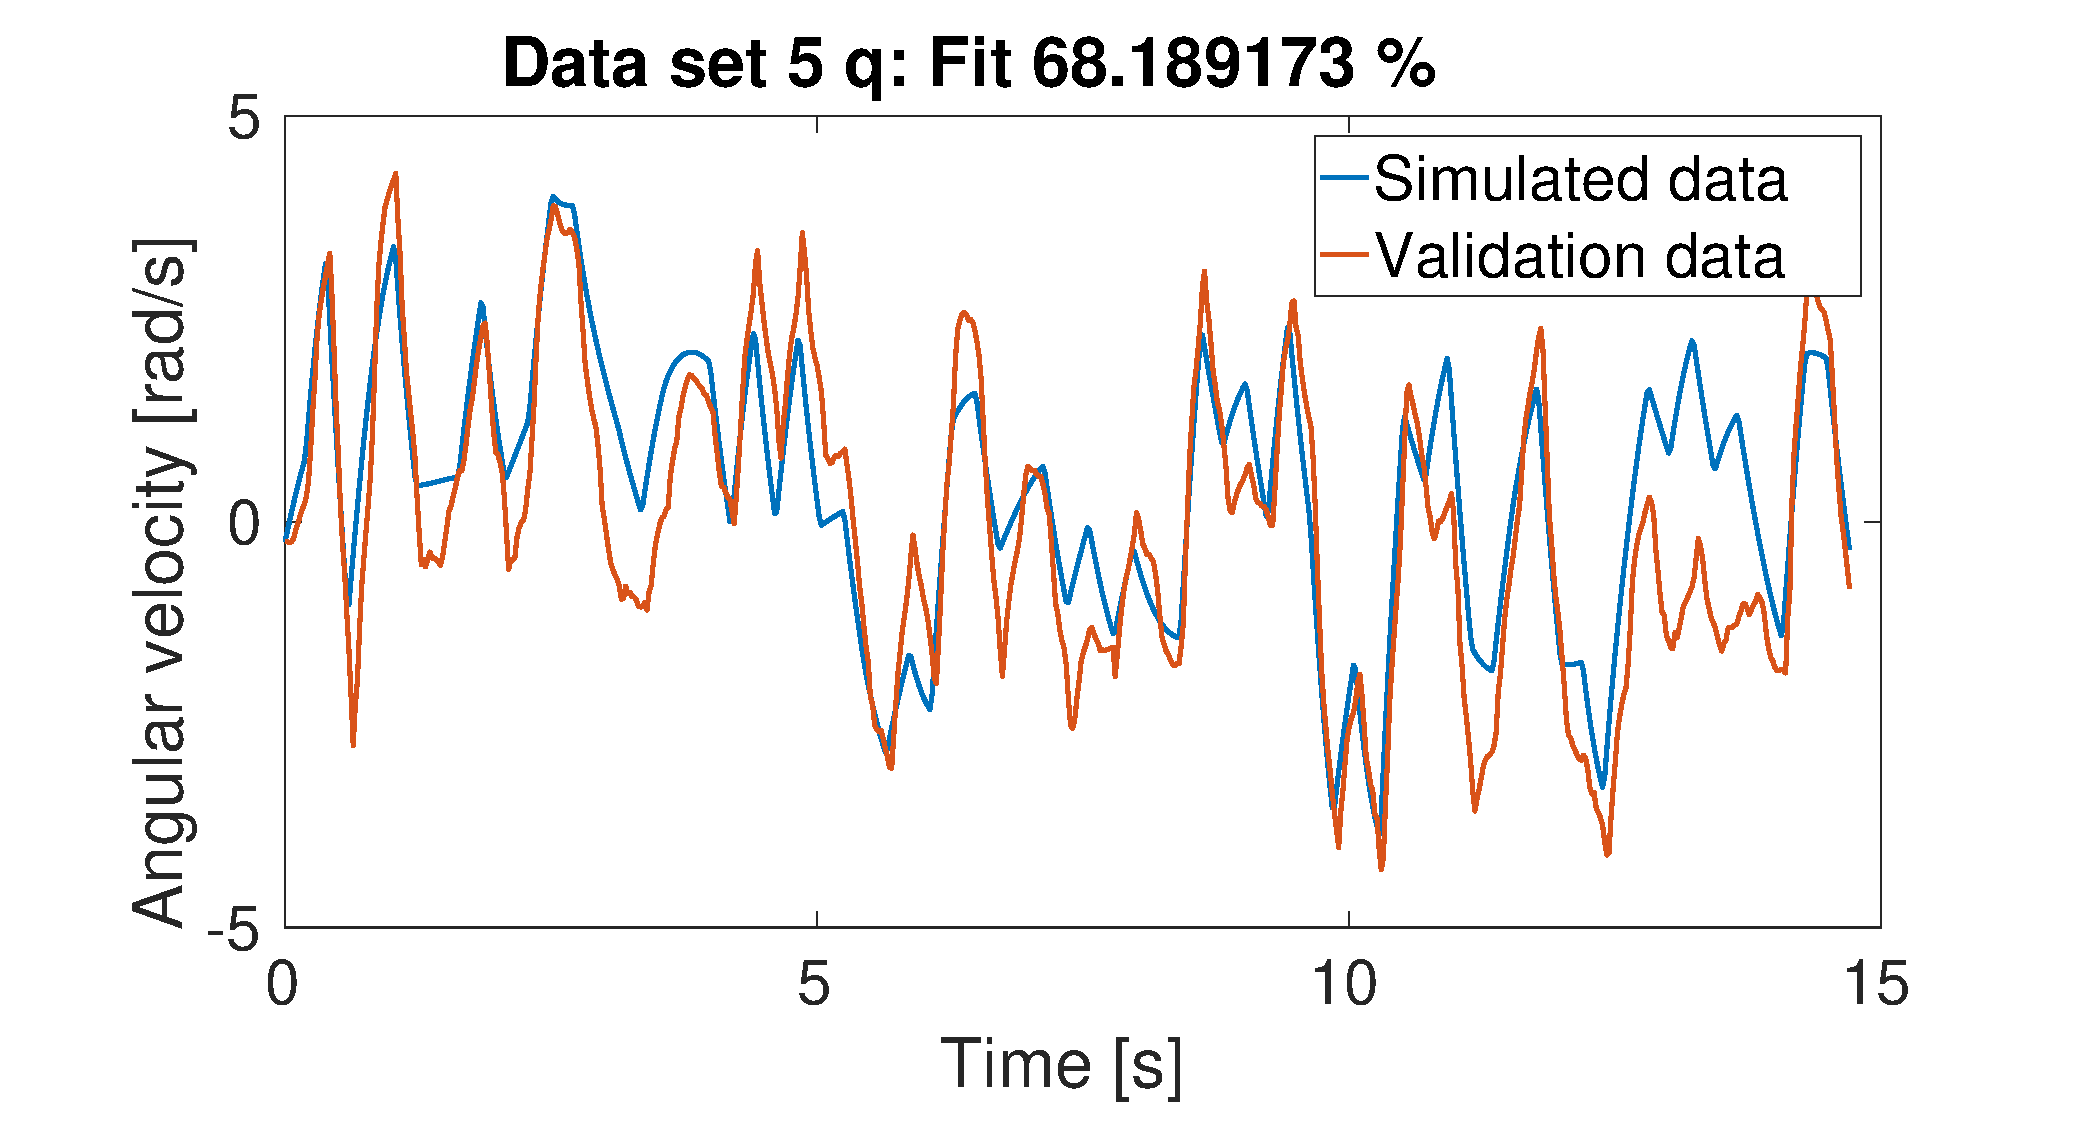
\includegraphics[width=0.7\textwidth]{ResultKalmanFixedMomentQ}}
  \\
  \subfloat[][Comparison between a simulated model response and validation data in $r$.]{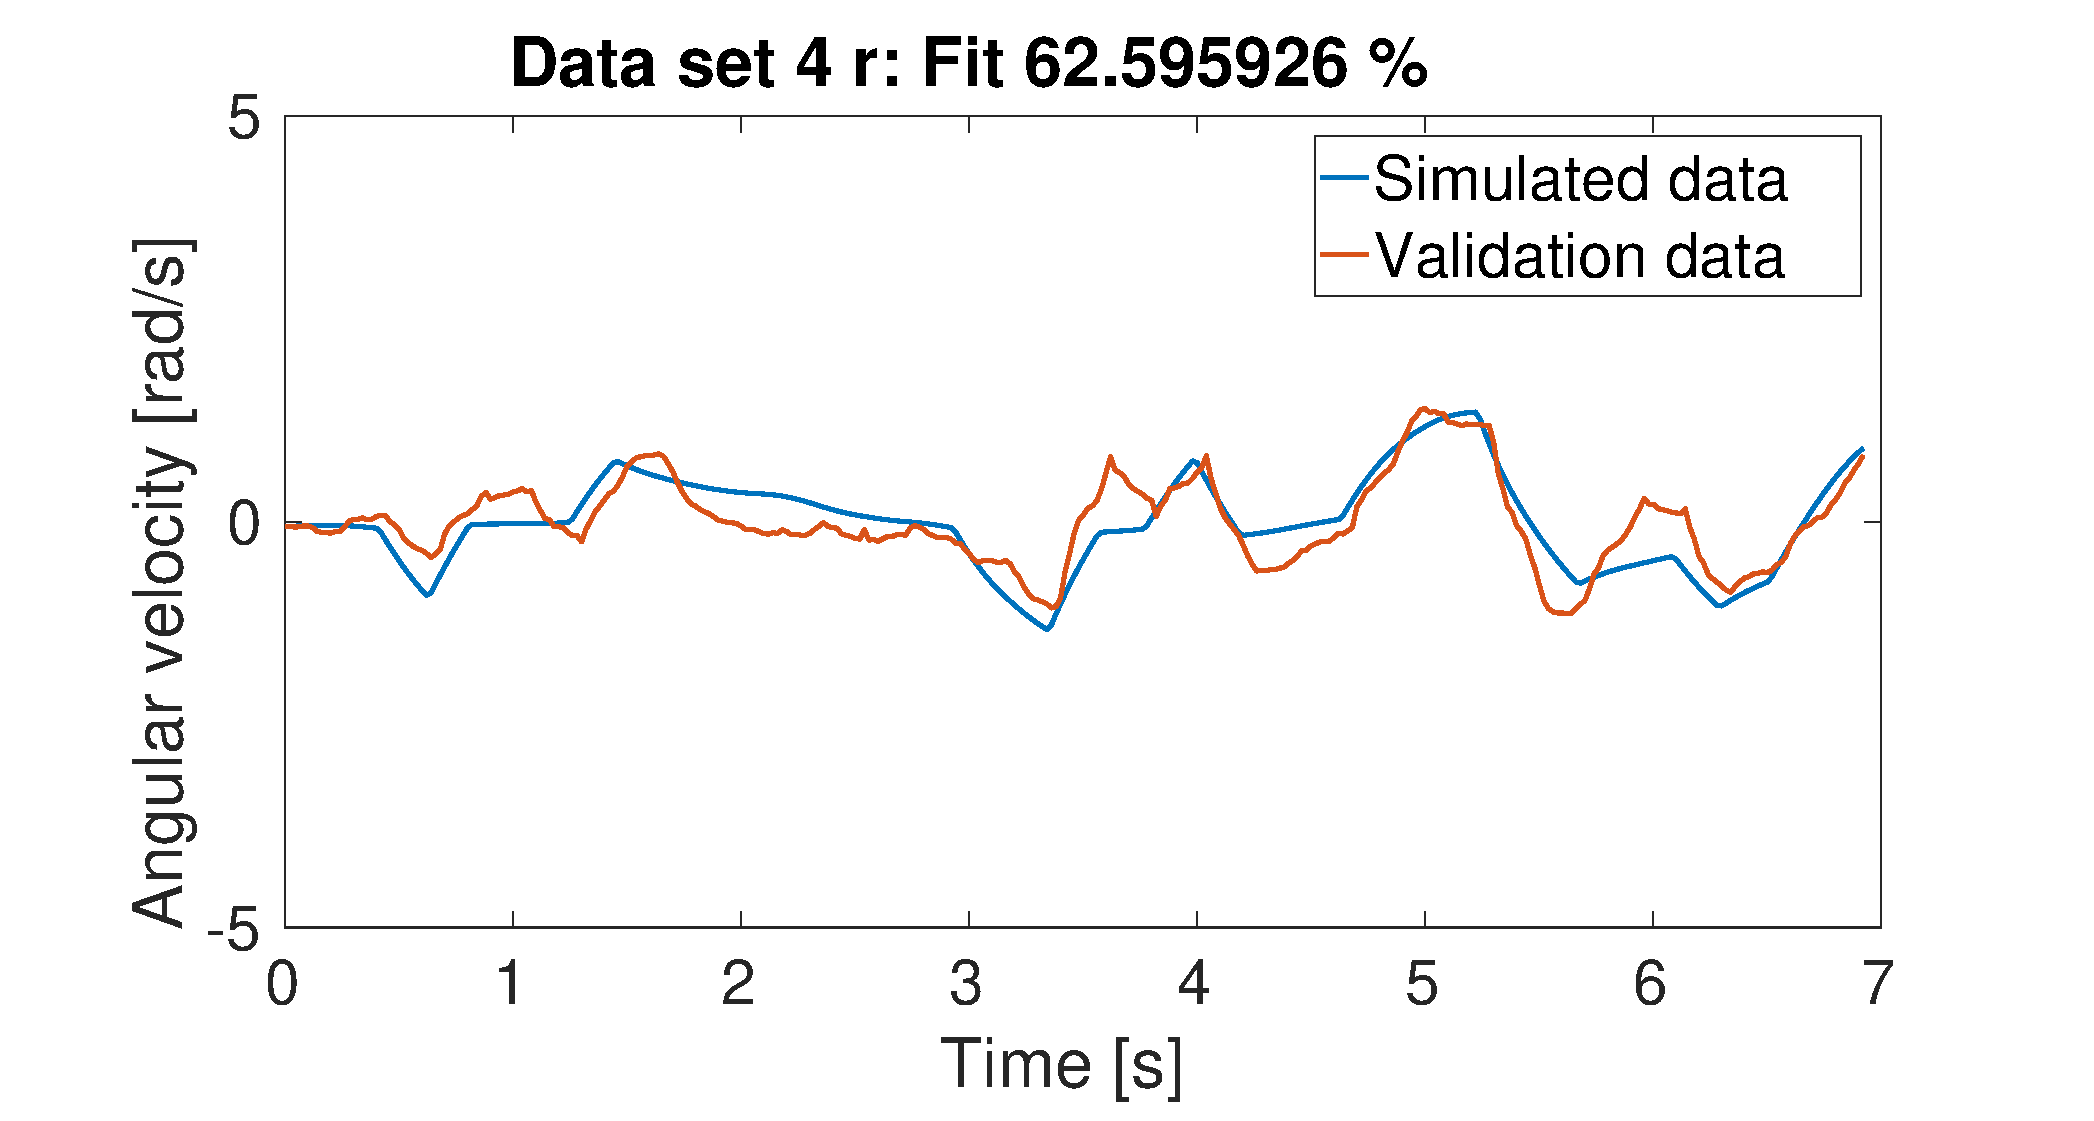
\includegraphics[width=0.7\textwidth]{ResultKalmanFixedMomentR}}
  \caption{\label{fig:ResultKalmanFixedMomentArms}%
    Comparison between simulation of $\nuVector$ (blue) with validation data (red). Moment-arm parameters are fixed. Goodness of fit statistic is displayed at the top of each sub-figure. The model describe the validation data well in $q$ and $r$ which can be seen in the high fit. The low fit in $p$ indicates that the model does not describe the validation data well.}
\end{figure}


\section{Investigating Low Fit in p Dynamics}
An issue that was present during both estimations methods was a low fit in $p$ during validations. This was further investigated by manually testing the each thruster and visual inspecting the response of the \abbrROV. During tests it was discovered that thruster 6, see \Figureref{fig:thrusterlocationfront}, had minimal effect in $p$. A test showed that thruster 6 only had significant effect in $p$ when it was actuated quickly. If the sixth thrusters power was incremented slowly an initial response in $p$ was noted before it settled close to zero again. The effect of thruster 6 in $p$ can be seen in \Figureref{fig:thruster6}. Thruster 6 also effected $r$, this can be due to unmodelled water interaction.

\begin{figure}
\centering
  \subfloat[][\label{fig:thruster6p1} The effect in $p$ when only using thruster 6.]{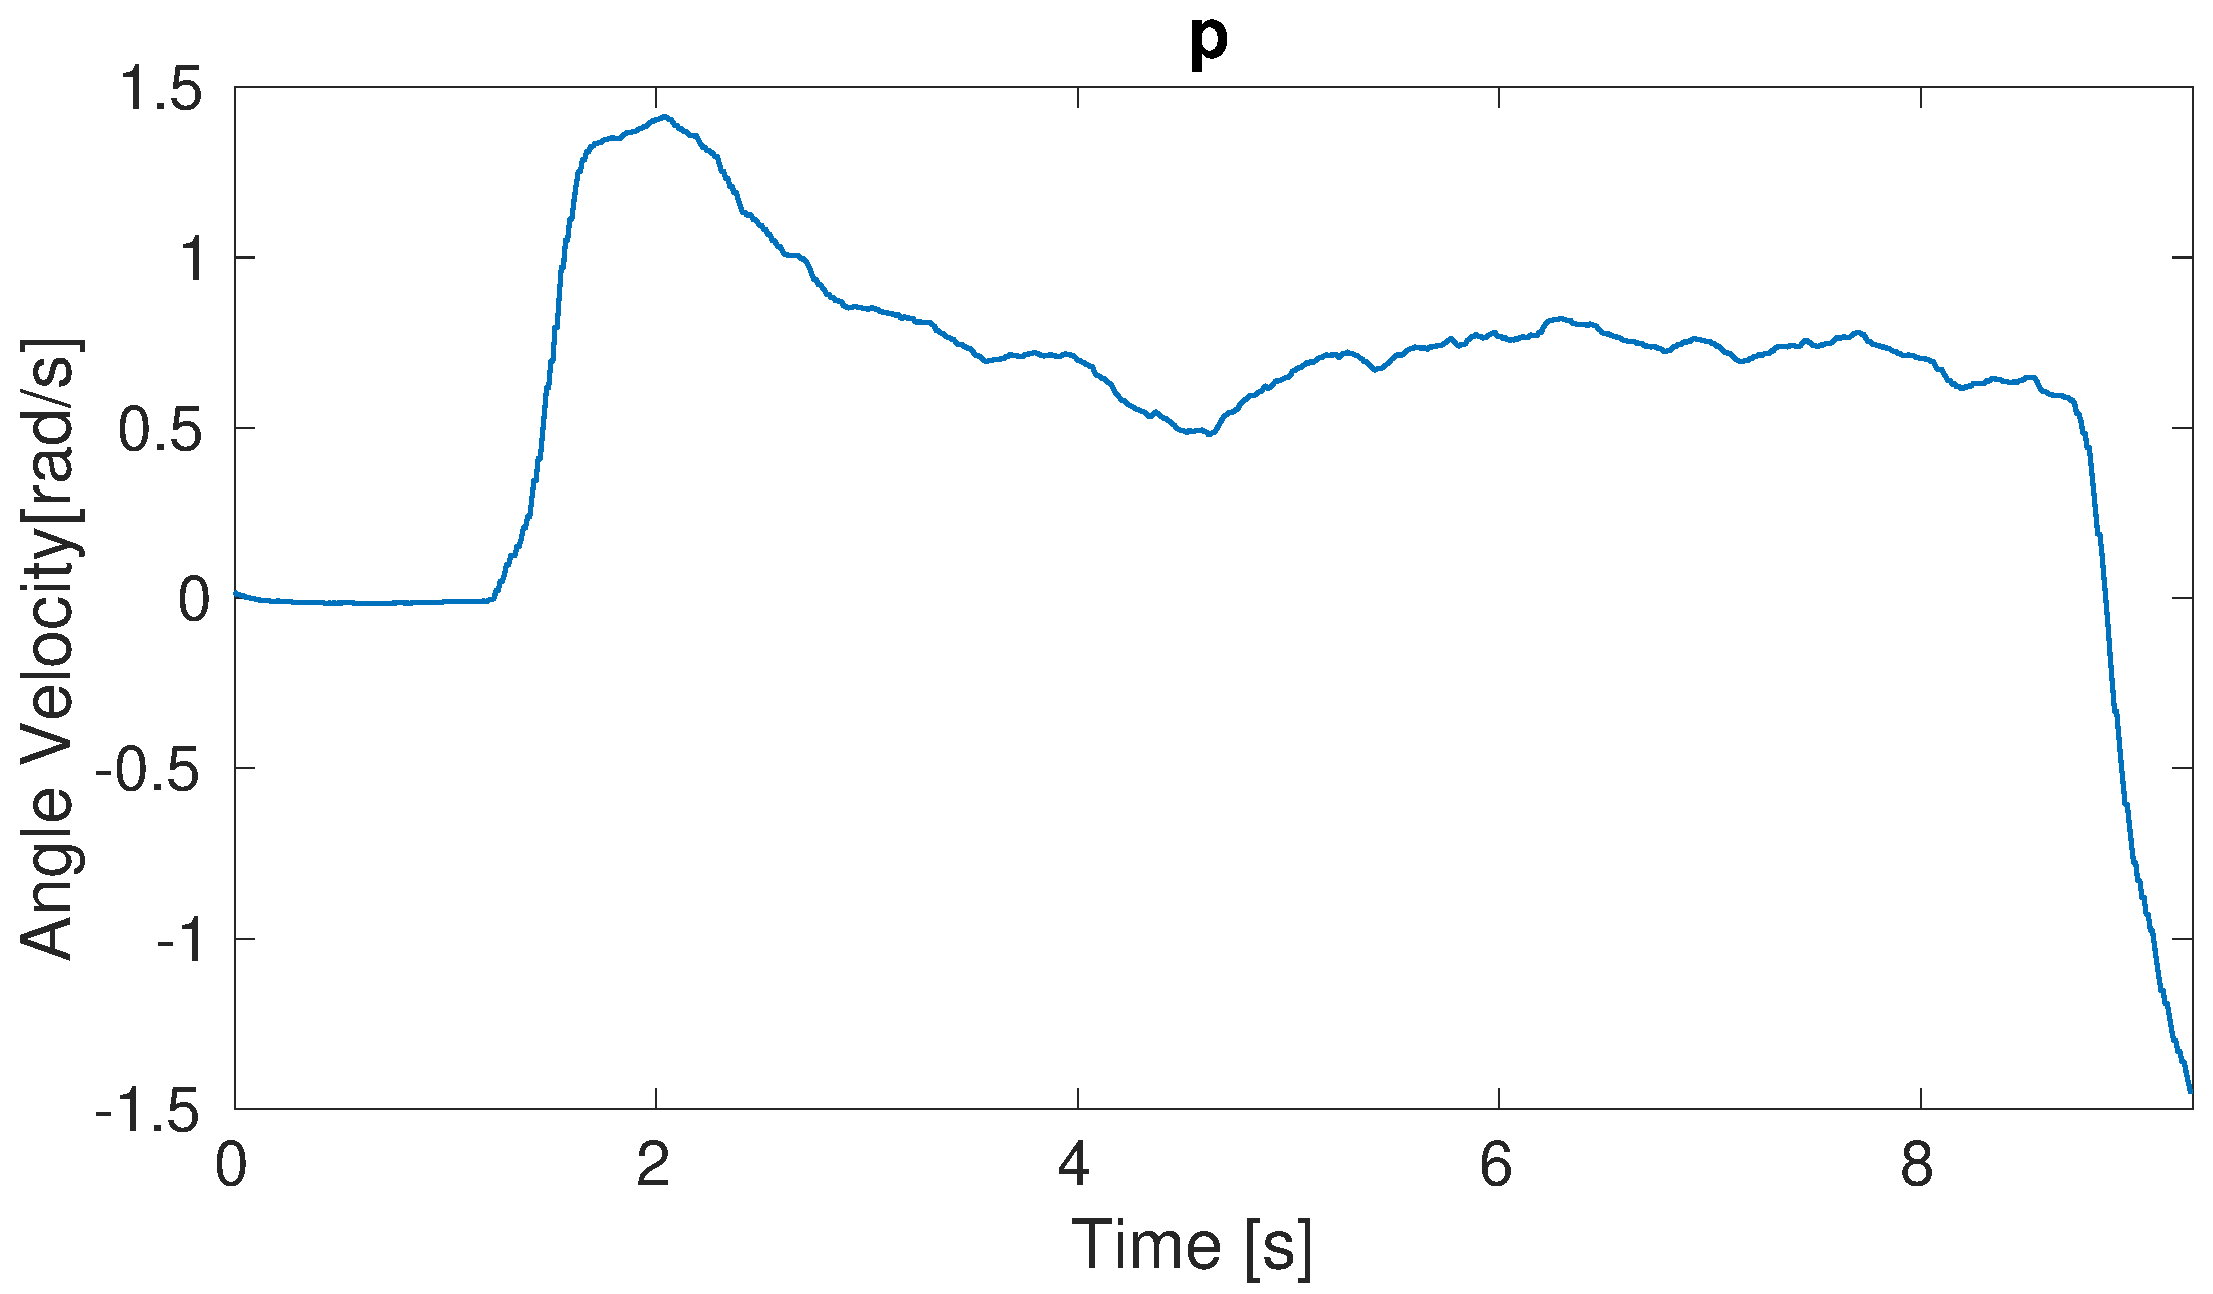
\includegraphics[width=0.4\textwidth]{thruster6p}}
  \qquad
  \subfloat[][\label{fig:thruster6u61} The effect in $r$ when only using thruster 6.]{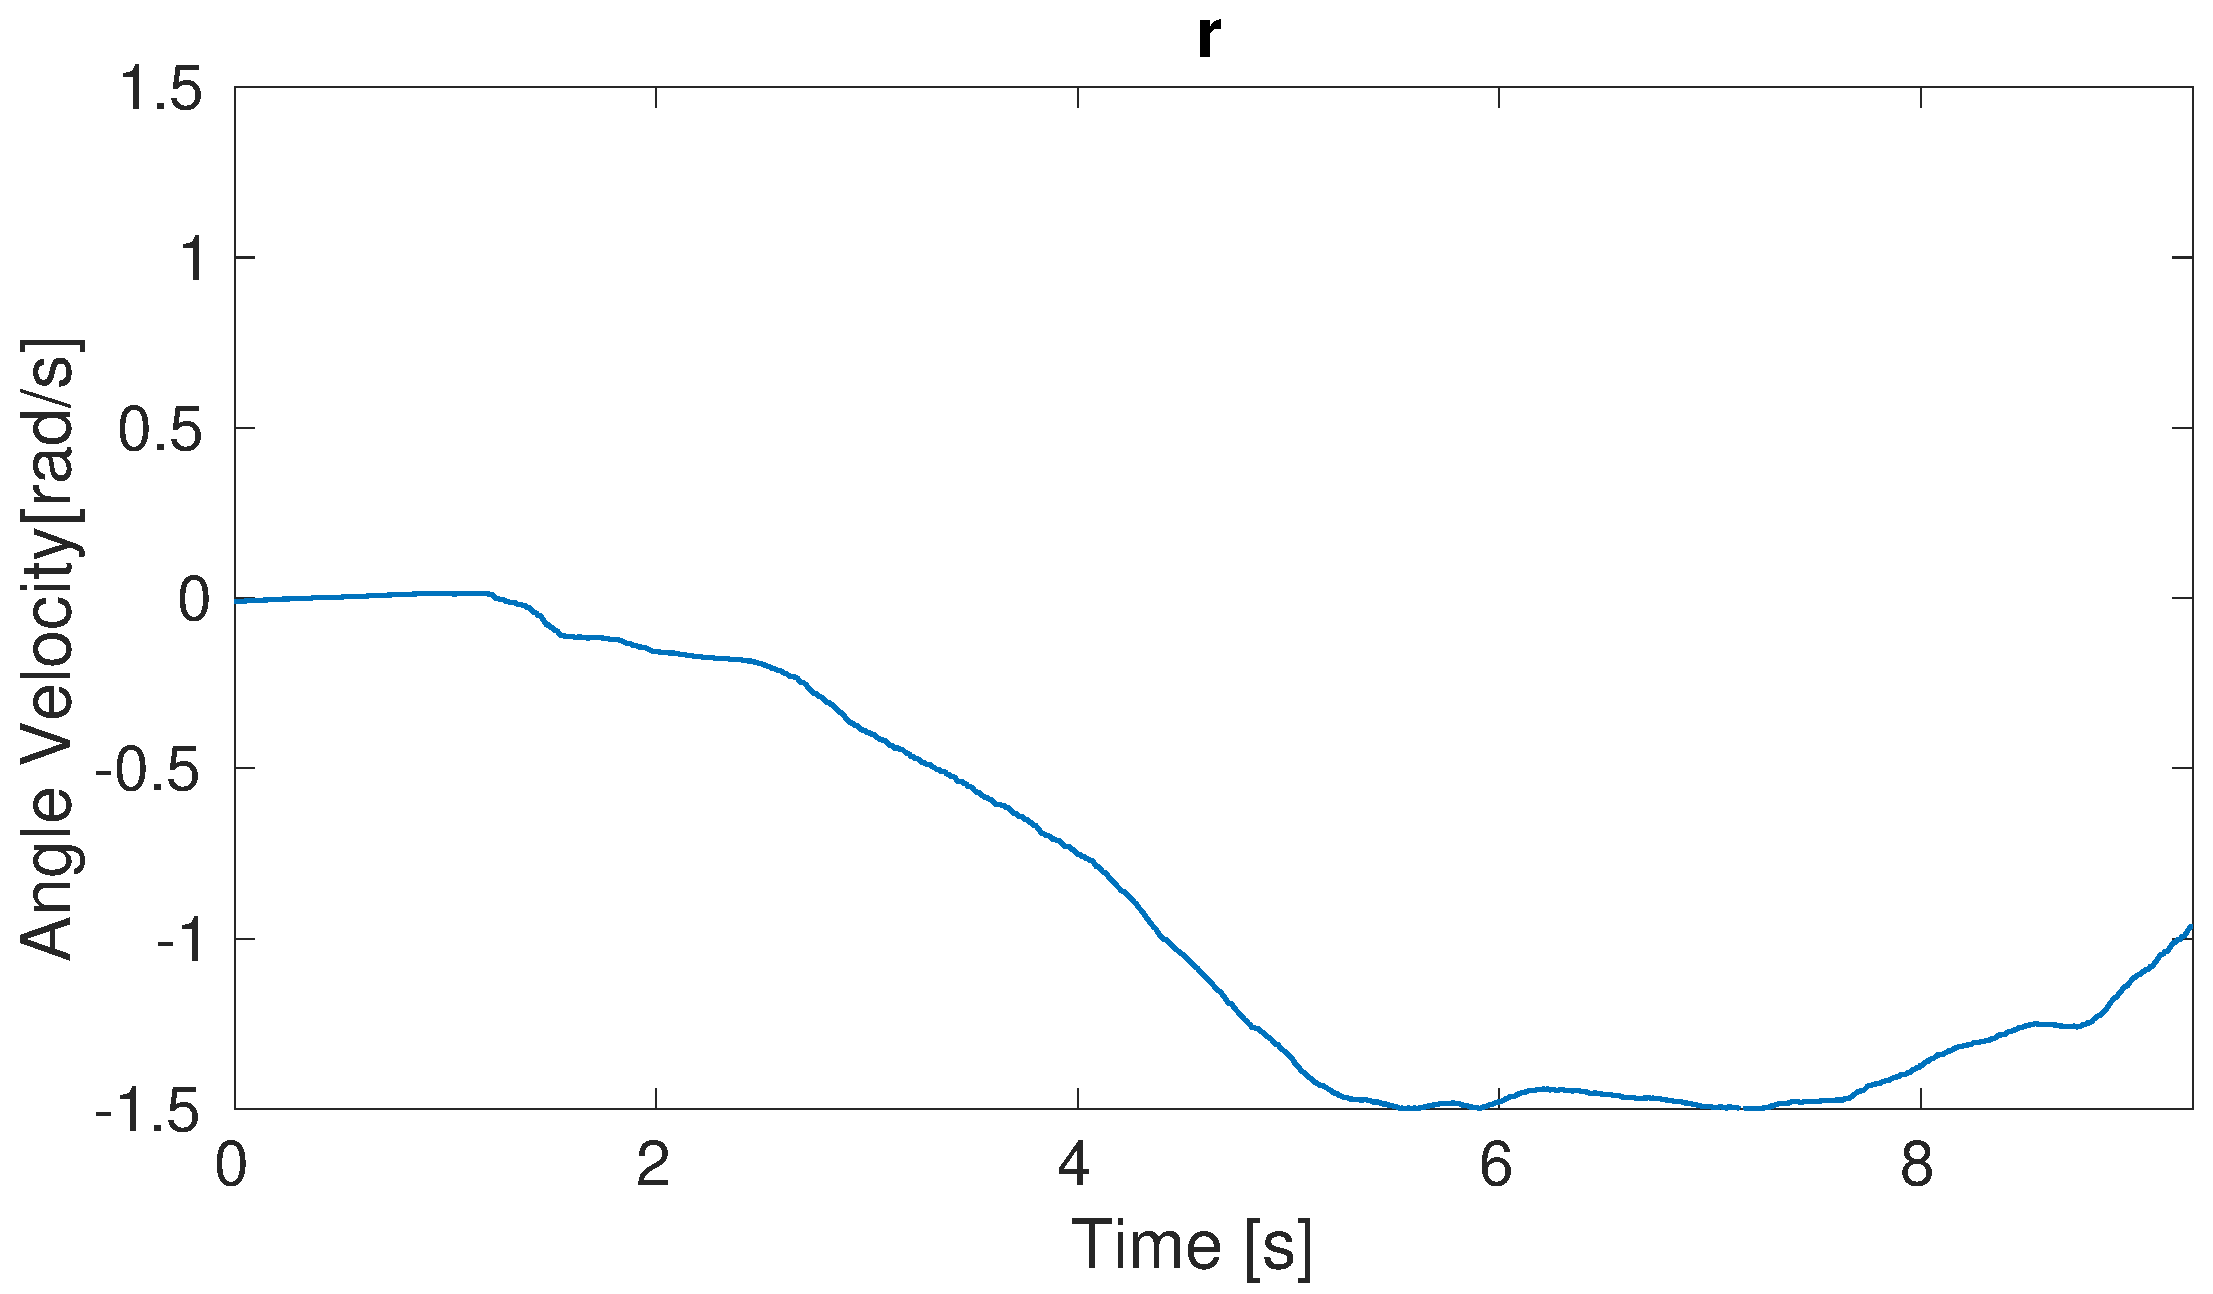
\includegraphics[width=0.4\textwidth]{thruster6r}}
  \qquad
  \subfloat[][\label{fig:thruster6r1} The control signal sent to thruster 6.]{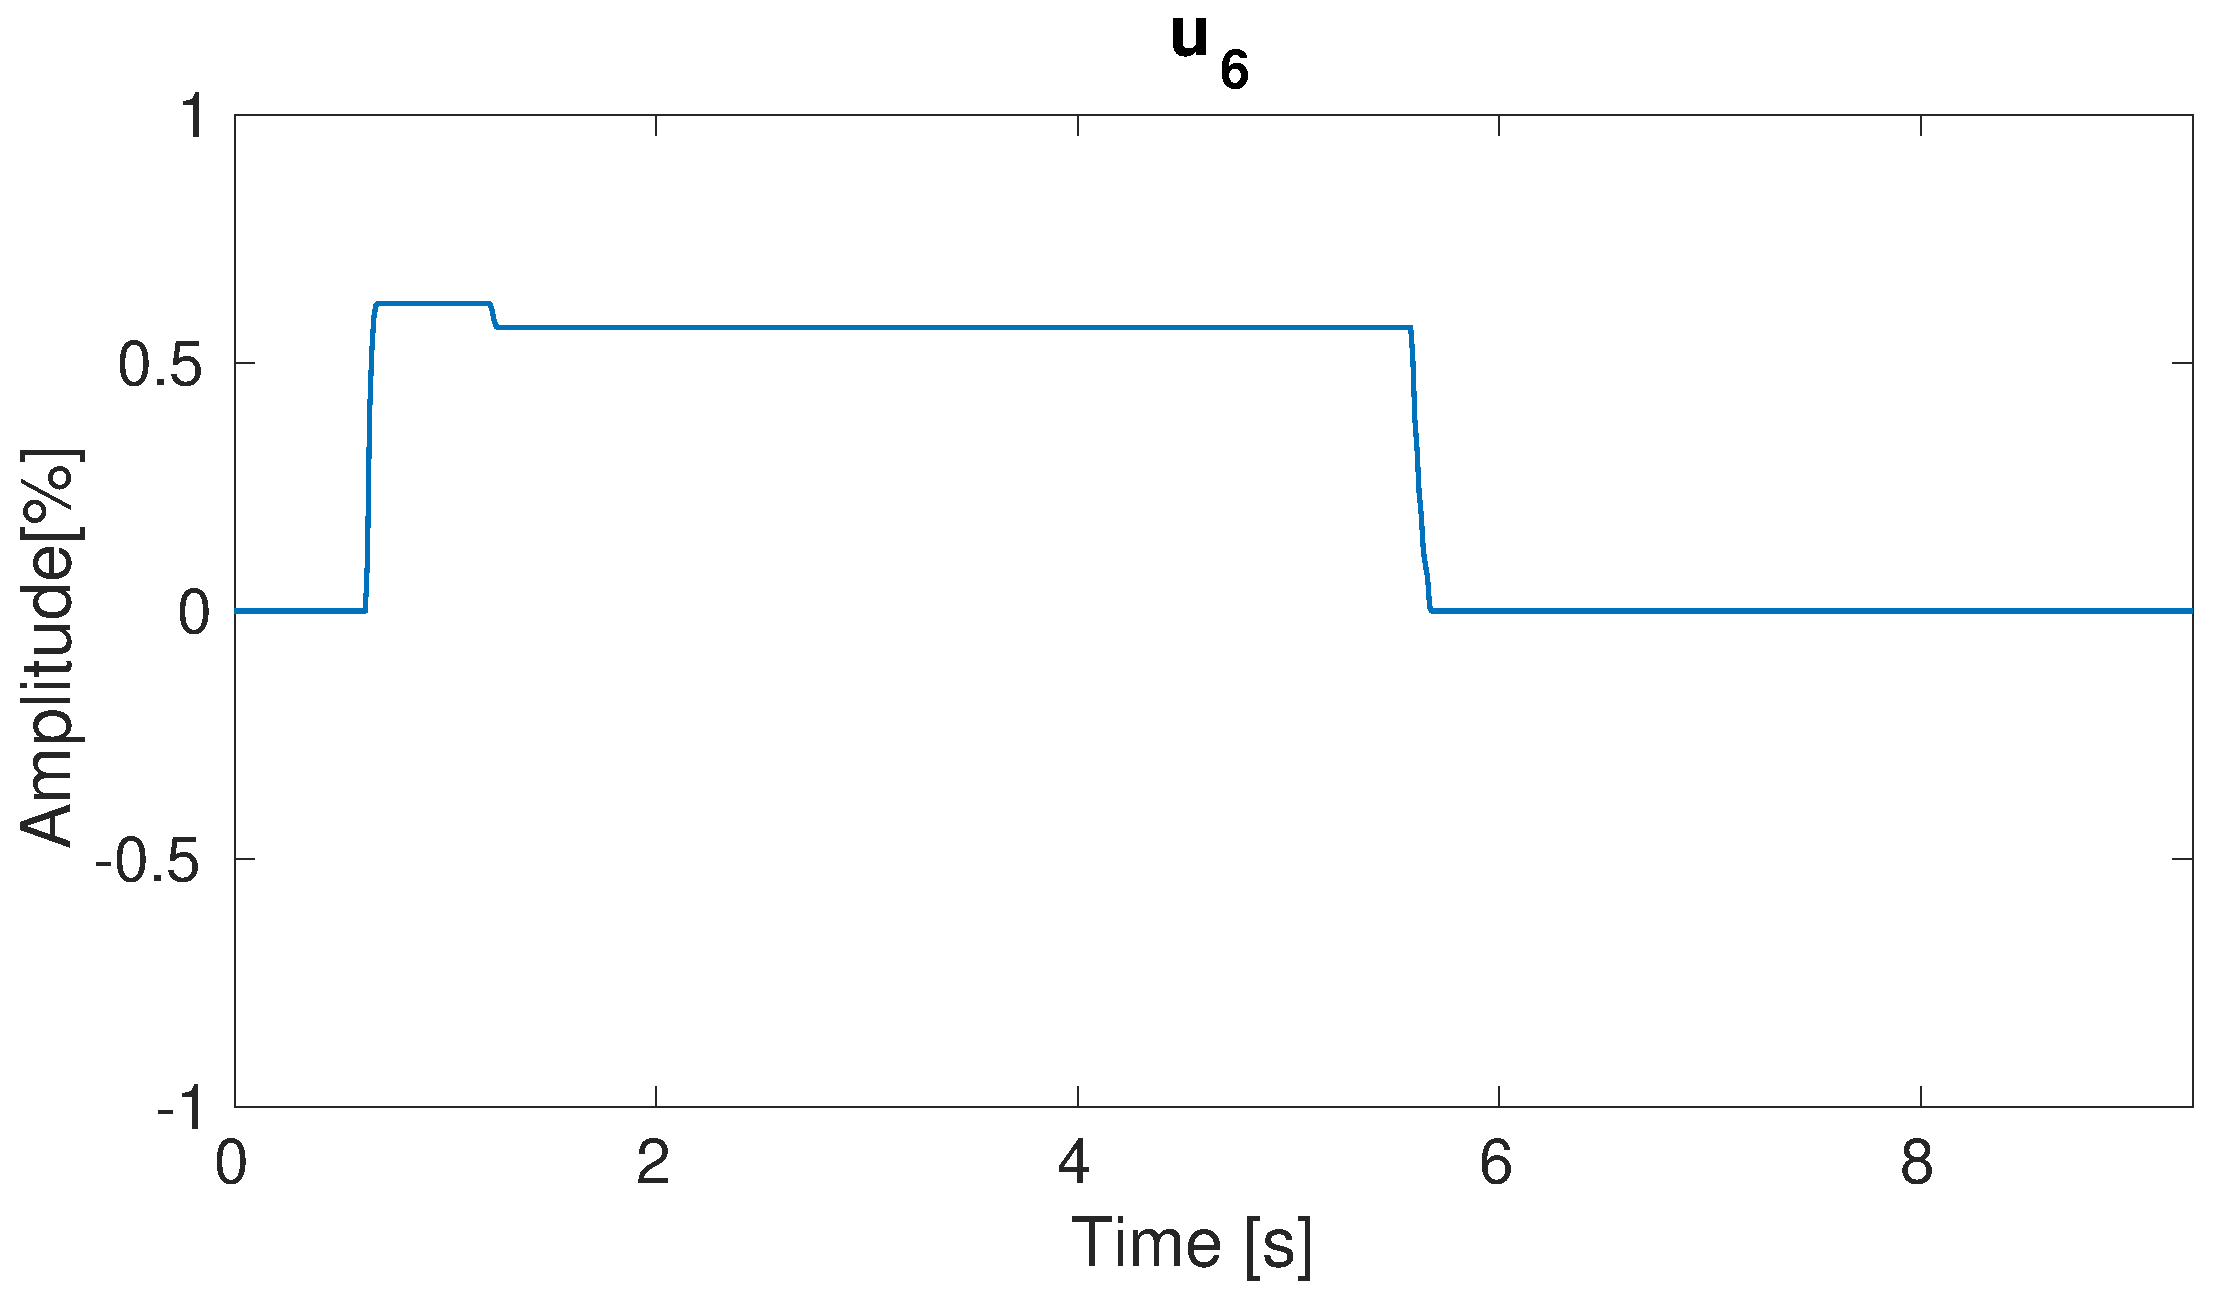
\includegraphics[width=0.4\textwidth]{thruster6u6}}
  \caption{\label{fig:thruster6}%
  The effect in $p$ and $r$ while only using thruster 6. As can be seen thruster 6 has a relatively small effect in $p$, thus ought the moment arm of thruster 6 be small. However, thruster 6 effected $p$ more when thruster 6 was quickly actuated.}
\end{figure}

It was decided that thruster 6 was to be eliminated from the estimation, and a second estimation was run with the moment arm for thruster 6 $\distance{z}{6}$ fixed to zero. The filter was once again initialised with the following settings
\begin{equation*}
\boldsymbol{Q}=\text{diag}[\underbrace{\overbrace{1000}^{\times4}}_{\etaVector}... \underbrace{\overbrace{1000}^{\times3}}_{\nuVector}...\underbrace{\overbrace{0.01}^{\times3}}_{\boldsymbol{b}}... \underbrace{\overbrace{0.001}^{\times10}}_{\boldsymbol{\theta}}]
\end{equation*}
and
\begin{equation*}
\boldsymbol{R} = \text{diag}[\underbrace{\overbrace{0.001}^{\times3}}_{\text{Gyro}}... \underbrace{\overbrace{0.1}^{\times3}}_{\text{Acc}}... \underbrace{\overbrace{1000}^{\times3}}_{\text{mag}}]
\end{equation*} 
The estimation was done with five data sets, of which the first three were used for estimation while the fourth and fifth were used for validation. The estimator was iterated 2 times, using the parameter values from the previous iteration as the new initial states. The resulting parameter values and their initial values can be viewed in \tableref{tab:ResultKalmanFixedMomentArmsLz6} and a comparison of a simulated run against validation data is shown in \figureref{fig:ResultKalmanFixedMomentArmsLz6}. As can clearly be seen in \Figureref{fig:ResultKalmanFixedMomentArmsLz6}, a drastic improvement in fit for $r$ is noted. A similar performance increase was achieved when using the prediction-error method with $\distance{z}{6}=0$. It is unclear what is causing thruster 6 to diminish the fit of the model, but there are some possible explanations. 

The assumption in \sectionref{cha:modelling}, that \abbrCG and the \abbrCO are placed at the same place in the \abbrROV may be invalid. If the \abbrCG is placed lower than the \abbrCO the measured moment arm of thruster 6 $\distance{z}{6}$ will be to long.  This will result in the effect in $p$ of thruster 6 to be less than expected. It could also be caused by the rotational center of the \abbrROV not located in the \abbrROV's \abbrCG. This is further strengthened by the fact that thruster 6 effect $r$.

% results kalman lz6=0 fixed moment arms
\begin{table}[hbp]
  \centering
  \caption{\label{tab:ResultKalmanFixedMomentArmsLz6}%
    The estimated parameters from the Kalman estimator method with moment arms fixed to measured values but with $\distance{z}{6}$ fixed to zero.}
  \begin{tabular}{l l p{0.25\linewidth}}
    \toprule%
    \textbf{Notation}  & \textbf{Starting Value} & \textbf{Estimated Value} \\
    \otoprule%   
    % Parameters that will be estimated
    $\etaVector$			&$[1\ 0\ 0\ 0]^T$					&\\
    $\nuVector$			&$[0\ 0\ 0]^T$						&\\
    $\boldsymbol{b}$					&$[0\ 0\ 0]^T$			&\\
	$z_B$               & -0.05	\meter 						& -0.0420 	\meter\\
    $\Kp$               & -1   	\kilogram\usk\meter\squared 	& -0.8842 		\kilogram\usk\meter\squared\\
    $\Kpabsp$           & -1  	\kilogram\usk\meter\squared	& -0.6682  		\kilogram\usk\meter\squared\\
    $\Mq$               & -1  	\kilogram\usk\meter\squared	& -0.8547  		\kilogram\usk\meter\squared\\
    $\Mqabsq$           & -1  	\kilogram\usk\meter\squared	& -0.3354  	\kilogram\usk\meter\squared\\
    $\Nr$               & -1  	\kilogram\usk\meter\squared	& -1.0280		\kilogram\usk\meter\squared\\
    $\Nrabsr$           & -1  	\kilogram\usk\meter\squared	& -1.0249 		\kilogram\usk\meter\squared\\
    $A_p$               & 1 	\kilogram\usk\meter\squared	&  0.8337 		\kilogram\usk\meter\squared\\
    $B_q$               & 1 	\kilogram\usk\meter\squared	&  0.7987		\kilogram\usk\meter\squared\\
    $C_r$               & 1 	\kilogram\usk\meter\squared	&  1.1250		\kilogram\usk\meter\squared\\
    \bottomrule%
  \end{tabular}
\end{table}

% results kalman lz6=0 fixed moment arms
\begin{figure}[tbp]
  \centering
  \subfloat[][Comparison between a simulated model response and validation data in $p$.]{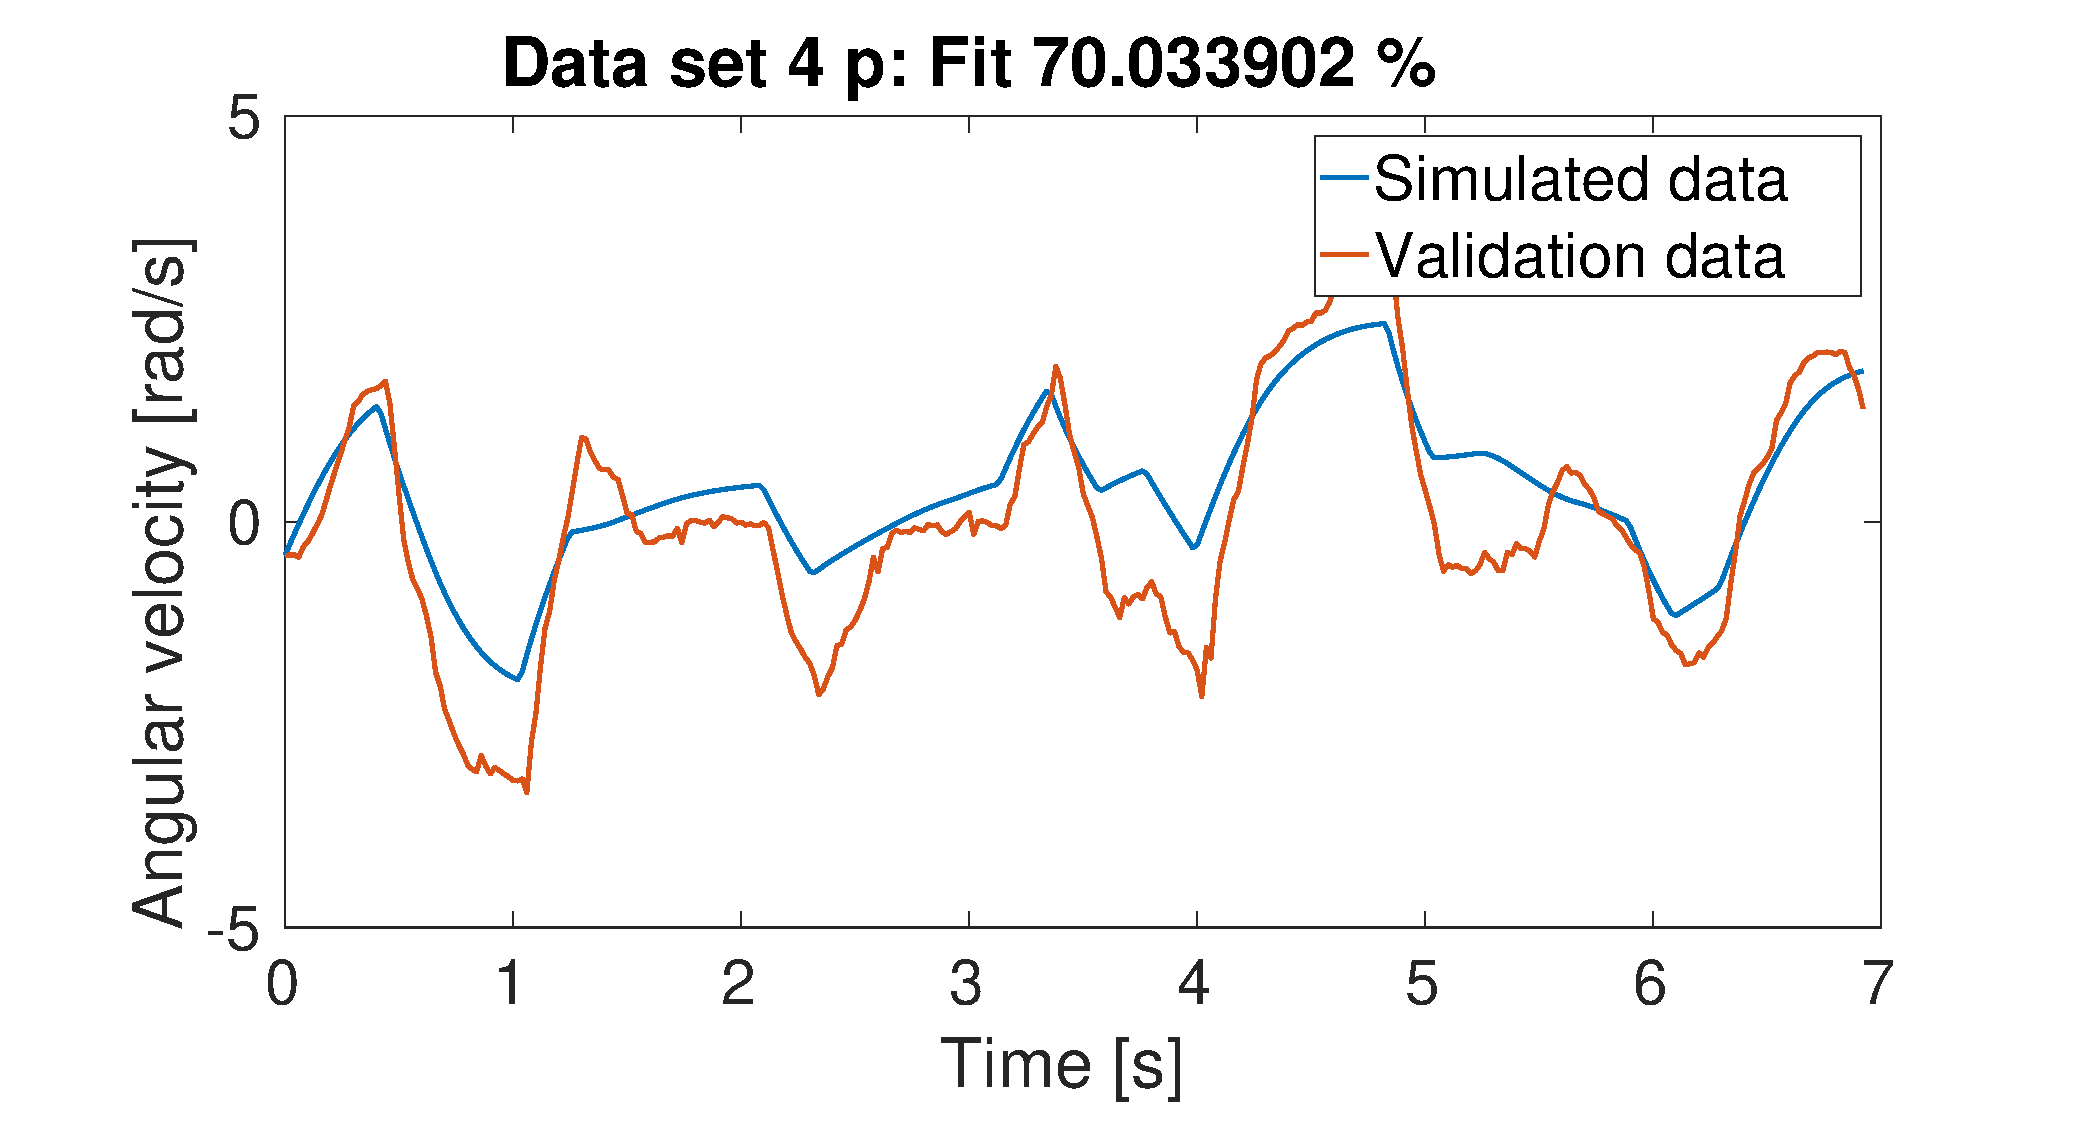
\includegraphics[width=0.7\textwidth]{ResultKalmanFixedMomentPLz0}}
  \qquad
  \subfloat[][Comparison between a simulated model response and validation data in $q$.]{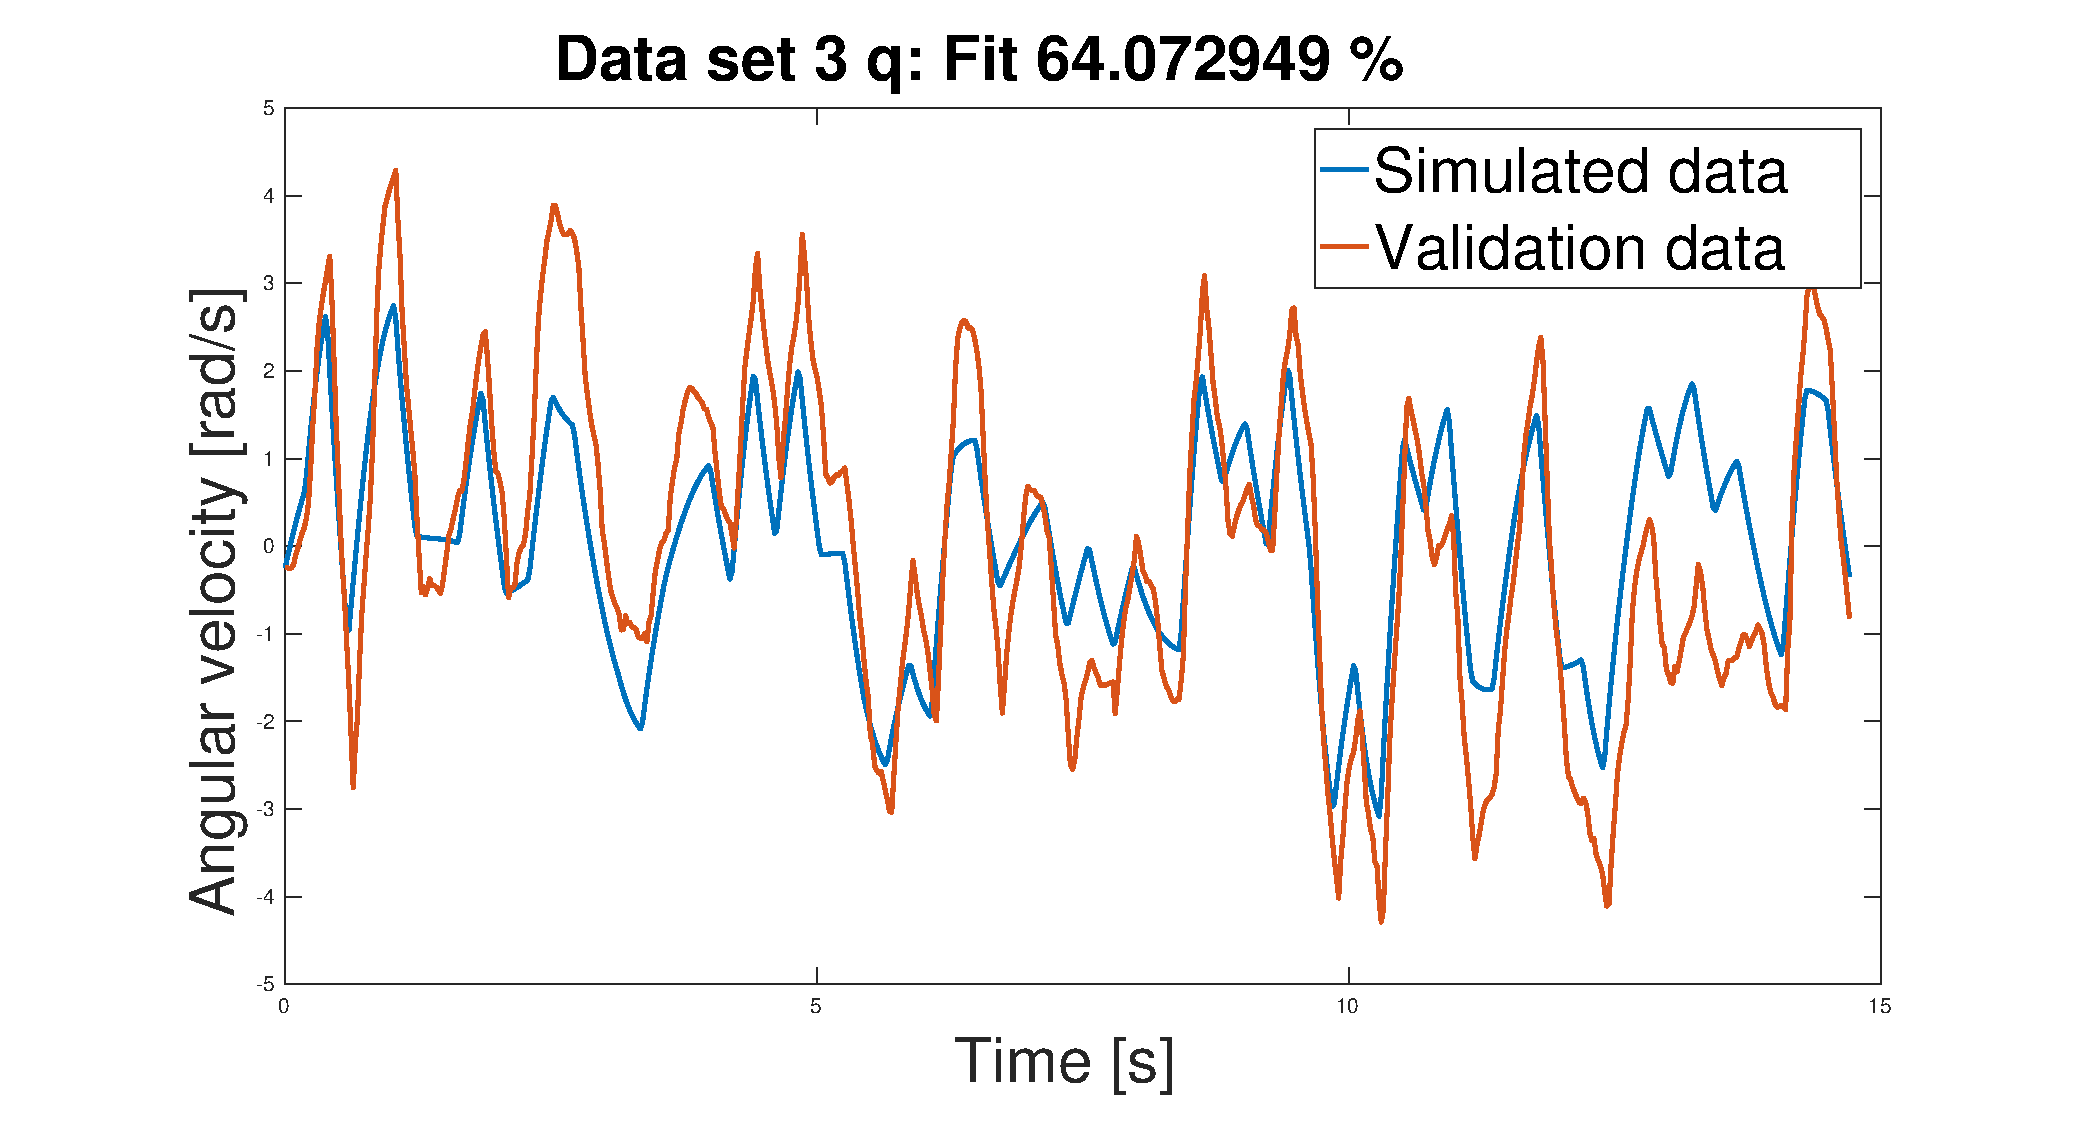
\includegraphics[width=0.7\textwidth]{ResultKalmanFixedMomentQLz0}}
  \\
  \subfloat[][Comparison between a simulated model response and validation data in $r$.]{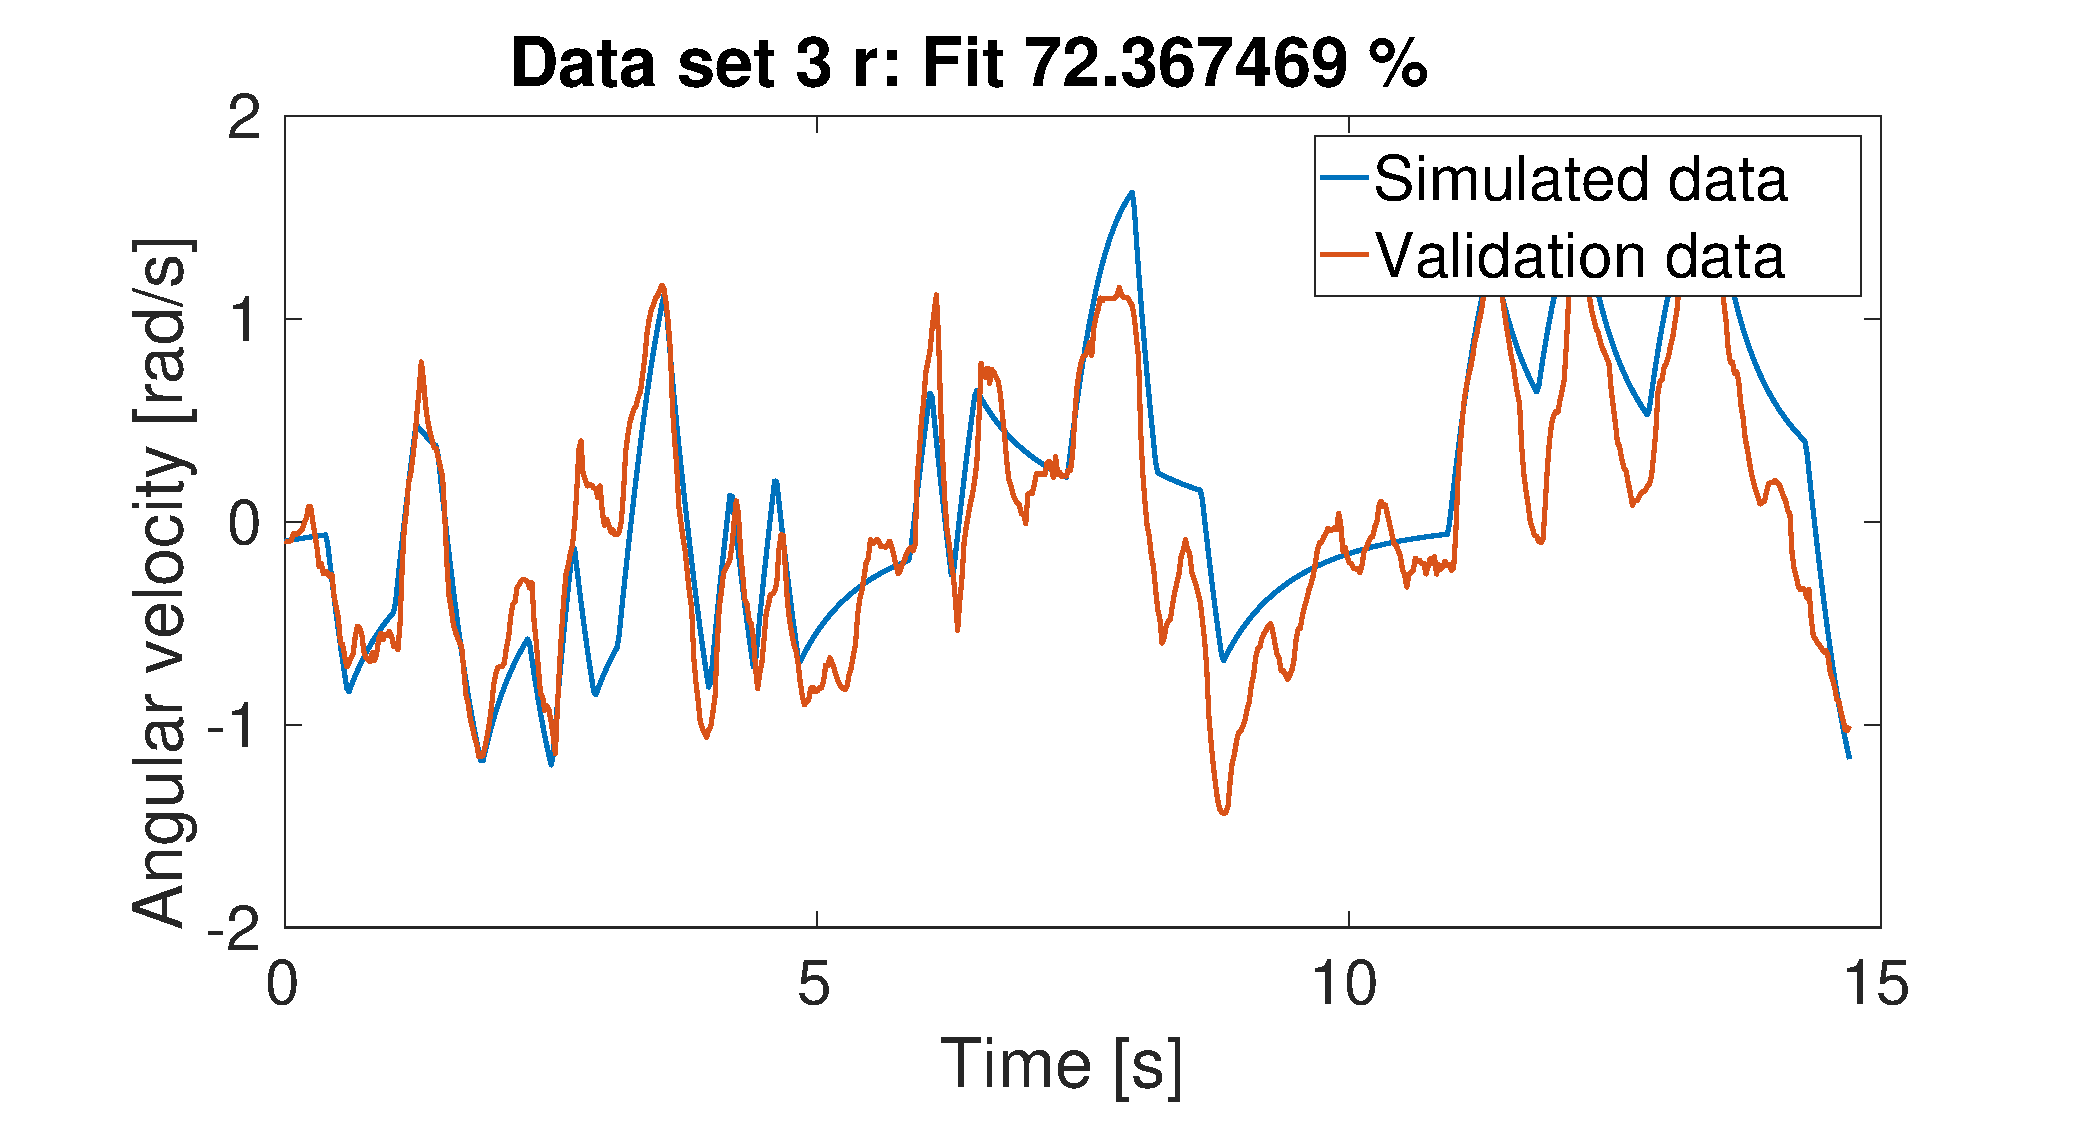
\includegraphics[width=0.7\textwidth]{ResultKalmanFixedMomentRLz0}}
  \caption{\label{fig:ResultKalmanFixedMomentArmsLz6}%
    Comparison between simulation of $\nuVector$ (blue) with validation data (red). Moment-arm parameters are fixed and \distance{z}{6} is set to zero. Goodness of fit statistic is displayed at the top of each sub-figure.}
\end{figure}


%\section{Discussion}
%To estimate parameters in the reduced 6-\abbrDOF model was harder than it at first seemed. Problems were encountered when the prediction-error method was used with bad fit in $p$. 
%When deciding on which parameters to use for controller design, the choice was based solely on the fit of the simulated output had against validation data. The reasoning behind this being quite simple, the better the fit against validation data the less robust the controllers would have to be.
%%%%%%%%%%%%%%%%%%%%%%%%%%%%%%%%%%%%%%%%%%%%%%%%%%%%%%%%%%%%
%\section{Decoupling the Model} \index{Decoupling}
% From \eqref{eq:WithoutTranslation} it can be seen that $r$ is not affected by the same thrusters as $p$ and $q$. Thus the $r$ model's parameters were initially estimated by themselves while the parameters in the $p$ and $q$ models were estimated together. 
%
%The estimation of the attitude model structure was divided into three estimation steps.
%
%The separately estimated parameters were then used as starting values for a complete attitude model parameter estimation, \eqref{eq:WithoutTranslation}. The reduced models for $r$, $p$ and $q$ that were used during initial estimation were
%
%The simplification could be done since excitation in the states not used in a particular estimation were kept at a minimum during data collection. Thus the coupled terms in each equation were approximated to be zero.

%%%%%%%%%%%%%%%%%%%%%%%%%%%%%%%%%%%%%%%%%%%%%%%%%%%%%%%%%%%
%\section{Parameter Estimation from Angular Velocities} \label{sec:estimation_angular}
%The estimated Euler angles from the sensor fusion model described in \Sectionref{sec:simple_model} did not follow the kinematic relation described in \Sectionref{sec:kinematics} which can be seen in \Figureref{fig:integratedAngleVelocities}. This also meant that the angles were unfit for use in as outputs in the parameter estimation since the angle estimates will not describe the system well since the estimates include the \abbrEKF's dynamics. The parameters were instead estimated using the angular velocities from the gyroscope as outputs an with the estimated euler angles as inputs. The model structure in which the parameters were estimated was thus \index{model structure}
%\begin{equation}
%\etaVectordot = f(\nuVector, \hat{\etaVector}, \tauVector),
%\end{equation}
%and
%\begin{equation}
%\boldsymbol{y} = \nuVector
%\end{equation}
%where $\hat{\etaVector}$ contains the estimated Euler angles from the sensor fusion.
%
%
%
%To get an initial estimate on the parameters in the yaw dynamics the reduced model parameters in \eqref{eq:r_dot_decouple}
%were estimated using data collected from a test that mainly excited the \abbrROV in $r$ which can be seen in \Figureref{r_rTest}.
%
%Since the dynamics in $p$ and $q$ are coupled \eqref{eq:pq_dot_decouple1} and \eqref{eq:pq_dot_decouple2} needed to be estimated at the same time. The cross terms in $r$ was assumed to be zero since the \abbrROV was mainly excited in $p$ and $q$ during collection of the used estimation data which can be seen in \Figureref{p_qTest}.
%
%The initial estimates of the parameters in \eqref{eq:pq_dot_decouple1} and \eqref{eq:r_dot_decouple} were used as initial estimates of the parameters in \eqref{eq:WithoutTranslation}. Due to observational problems the reparametrisation $A_p = \Ix - \Kpdot$, $B_q = \Iy - \Mqdot$ and $C_r = \Iz - \Nrdot$ was introduced. The fit can be seen in \Figureref{fig:velocityCompareCong} where the reparameterisation has been used.
%\index{Reduced model structure}
%
%%%%%%%%%%%%%%%%%%%%%%%%%%%%%%%%%%%%%%%%%%%%%%%%%%%%%%%%%%%%
%\section{Parameter Estimation from Angular Velocities and Linear Accelerations} \label{sec:angLinEstim}
%The parameters were also estimated using the angular velocities and the linear accelerations as outputs. This was done to avoid modelling the low-pass filtering effects in the sensor fusion described in \Chapterref{cha:sensor_fusion}. The model structure was modified to use quaternions instead of euler angles. Using quaternions in the model \eqref{eq:p_dotWithoutTranslation} - \eqref{eq:r_dotWithoutTranslation} with the reparameterision from \Sectionref{sec:estimation_angular} gave the model structure \todo{move model def to model chapter}
%\begin{multline}
%\pdot = \frac{\thrusterfun{1} \distance{y}{1} - \thrusterfun{2} \distance{y}{2} + \thrusterfun{6} \distance{z}{6}}{A_p} + \frac{B z_B (2 \quatII \quatIII + 2 \quatI \quatO)}{A_p} + \\ \frac{p (\Kp + \Kpabsp \abs{p})}{A_p} + \frac{q r (B_q - C_r)}{A_p},
%\end{multline}
%\begin{multline}
%\qdot = \frac{\thrusterfun{1} \distance{x}{1} + \thrusterfun{2} \distance{x}{2} - \thrusterfun{5} \distance{x}{5}}{B_q} - \frac{B z_B (2 \quatI \quatIII - 2 \quatII \quatO)}{B_q} + \\ \frac{q (\Mq + \Mqabsq \abs{q})}{B_q} - \frac{p r (A_p - C_r)}{B_q}
%\end{multline}
%and
%\begin{multline}
%\rdot = \frac{\thrusterfun{3} \distance{y}{3} - \thrusterfun{4} \distance{y}{4}}{C_r} + \frac{r (\Nr + \Nrabsr \abs{r}}{C_r} + \frac{p q (A_p  - B_q)}{C_r}
%\end{multline}
%
%Thus the model structure in which the parameters was estimated became \index{model structure}
%\begin{equation}
%\etaVectordot = J(\etaVector) \nuVector,
%\end{equation}
%\begin{equation}
%\dot{\nuVector} =  f(\etaVector, \nuVector, \tauVector)
%\end{equation}
%with 
%\begin{equation}
%\boldsymbol{y} = \begin{bmatrix}
%\etaVector \\
%\boldsymbol{a}
%\end{bmatrix}
%\end{equation}
%where $\boldsymbol{a}$ are the linear accelerations in the \abbrROV frame. 
%
%The fit of the model compared to validation data can be seen in \Figureref{fig:angVelCompare}. To properly estimate the parameters the initial states had to be well estimated. The importance of a correct initial state estimate can be seen in \Figureref{fig:angVelSim}. Here the estimator was fed simulated data and was initialised with the true parameter values but had to estimate the starting state.   The estimated starting state was not well estimated, which in turn led to the parameters diverging from the true parameters and a low fit. A Kalman smoother as described in \citet{Wallin} was used introduced in order to alleviate this problem. During initial state estimation using the Kalman smoother the magnetometer was added as a output to reduce the uncertainty of the initial quaternions.
%
%
%To handle noisy signals an error threshold was introduced. An error threshold means that after a breakpoint the cost function becomes linear instead of quadratic. This makes the parameter estimation less sensitive to outliers. To reduce the impact of the noise even further the used weight matrix in the cost function was the inverse of the estimated noise covariance. 

%%%%%%%%%%%%%%%%%%%%%%%%%%%%%%%%%%%%%%%%%%%%%%%%%%%%%%%%%%%%
\section{Estimated Parameters}\label{sec:parameterResults}
\Tableref{tab:parameterConstants} shows the know, measured and estimated parameters used in the \abbrROV and controller development. These were chosen solely based on fit to validation data during simulation.

\begin{table}[tbp]
  \centering
  \caption{\label{tab:parameterConstants}%
    The known and estimated parameters used in the \abbrROV model.}
  \begin{tabular}{l l p{0.58\linewidth}}
    \toprule%
    \textbf{Notation}   & \textbf{Value} & \textbf{Description} \\
    \otoprule%
    $m$                 & 6.621 \kilogram                    & Mass of the \abbrROV. \\            
    $g$                 & 9.82  \meter\per\second\squared    & Gravity acceleration.\\   
    $\rho$              & 1000  \kilogram\per\meter\cubed    & Density of water.\\       
    
    $\distance{x}{1}$   & 0.19 \meter & Distance from \abbrCG to thruster 1 in $\xPosition$-direction.\\
    $\distance{y}{1}$   & 0.11 \meter & Distance from \abbrCG to thruster 1 in $\yPosition$-direction.\\
    $\distance{y}{2}$   & 0.11 \meter & Distance from \abbrCG to thruster 2 in $\yPosition$-direction.\\
    $\distance{x}{2}$   & 0.19 \meter & Distance from \abbrCG to thruster 2 in $\xPosition$-direction.\\
    $\distance{y}{3}$   & 0.11 \meter & Distance from \abbrCG to thruster 3 in $\yPosition$-direction.\\
    $\distance{x}{5}$   & 0.17 \meter & Distance from \abbrCG to thruster 5 in $\xPosition$-direction.\\
    $\distance{y}{4}$   & 0.11 \meter & Distance from \abbrCG to thruster 4 in $\yPosition$-direction.\\
    $\distance{z}{6}$   & 0    \meter & Distance from \abbrCG to thruster 6 in $\zPosition$-direction.\\
    	$z_B$               & -0.0420 \meter                                      & Distance from \abbrCG to \abbrCB.\\
    $\Kp$               & -0.8842 \kilogram\usk\meter\squared                 & Linear damping coefficient due to rotation in water about the $\xPosition$-axis.\\
    $\Kpabsp$           & -0.6682 \kilogram\usk\meter\squared                 & Quadratic damping coefficient due to rotation in water about the $\xPosition$-axis.\\
    $\Mq$               & -0.8547 \kilogram\usk\meter\squared                 & Linear damping coefficient due to rotation in water about the $\yPosition$-axis.\\
    $\Mqabsq$           & -0.3354 \kilogram\usk\meter\squared                 & Quadratic damping coefficient due to rotation in water about the $\yPosition$-axis.\\
    $\Nr$               & -1.0280 \kilogram\usk\meter\squared                 & Linear damping coefficient due to rotation in water about the $\zPosition$-axis.\\
    $\Nrabsr$           & -1.0249 \kilogram\usk\meter\squared                 & Quadratic damping coefficient due to rotation in water about the $\zPosition$-axis.\\
    $A_p$               & 0.8337  \kilogram\usk\meter\squared                 & Inertia around the $\xPosition$-axis and increased inertia around the $\xPosition$-axis.\\
    $B_q$               & 0.7987  \kilogram\usk\meter\squared                 & Inertia around the $\yPosition$-axis and increased inertia around the $\yPosition$-axis.\\
    $C_r$               & 1.1250  \kilogram\usk\meter\squared                 & Inertia around the $\zPosition$-axis and increased inertia around the $\zPosition$-axis.\\
    \bottomrule%
  \end{tabular}
\end{table}
\chapter{Controlling the ROV} \label{cha:controller} \index{Open-Loop Control} \index{Controller} \index{Exact Linearisation}
Automatic control is way of regulating a process without direct human interaction. The complexity can vary from decentralised proportional, integral and derivative controllers (\abbrPID:s) to more advanced model-based control methods, such as model predictive control (\abbrMPC). 

There are two main concepts of control, open-loop and feedback control. An open-loop controller is a controller that computes its output based on a model of the system and sometimes the current states. A disadvantage of open-loop controllers is that they require exact knowledge of the controlled system \citep{reglerteknik}. \Figureref{fig:control_system_open} illustrates the open-loop control scheme used in the \abbrROV. 

A feedback controller is a controller that uses measurements of the states in a system to correct its actions. One such method is error-controlled regulation, where the difference between the desired value, setpoint, of a state and its actual value is used for control. The feedback control scheme used in the \abbrROV can be seen in \Figureref{fig:control_system}. 

Similarly to an open-loop controller, a feedback controller can use a model of the system. Using a model of the controlled system in the control structure can produce better performance and compensate for unwanted effects such as non-linearities. Compensating for non-linearities is desired due to the fact that a lot of control principles are based on linear systems \citep{reglerteori}. 

\begin{figure}
	\centering
		\begin{tikzpicture}[auto, thick, node distance=2cm,>=latex',
			 block/.style  = {draw, rectangle,minimum height=3em, minimum width=6em},
			 sum/.style    = {draw, circle, inner sep=0pt, text width=4mm,align=center, node distance=1cm},
			 input/.style  = {coordinate},
			 output/.style = {coordinate},
			 pinstyle/.style = {pin edge={to-,thin,black}}]
			 
		    \node [input, name=input] {};
		    \node [block, right of=input, node distance=3cm] (controller) {F};
		    \node [block, right of=controller, node distance=3cm] (system) {\abbrROV};
		
		    \draw [->] (controller) -- node[name=u] {$u$} (system);
		    \node [output, right of=system] (output) {};
		
		    \draw [draw,->] (input) -- node {$u_{\text{control}}$} (controller);
		    \draw [->] (system) -- node [name=y] {$y$}(output);
		\end{tikzpicture}
	\caption{The open-loop control scheme used in the \abbrROV. The control block F can be any type of open-loop control. Notice that this is an ideal case were no disturbances affect the system.}
	\label{fig:control_system_open}
\end{figure}

\begin{figure}
	\centering
		\begin{tikzpicture}[auto, thick, node distance=2cm,>=latex',
			 block/.style  = {draw, rectangle,minimum height=3em, minimum width=6em},
			 sum/.style    = {draw, circle, inner sep=0pt, text width=4mm,align=center, node distance=1cm},
			 input/.style  = {coordinate},
			 output/.style = {coordinate},
			 pinstyle/.style = {pin edge={to-,thin,black}}]
			 
		    \node [input, name=input] {};
		    \node [sum, right of=input] (sum) {+};
		    \node [block, right of=sum] (controller) {F};
		    \node [block, right of=controller, node distance=3cm] (system) {\abbrROV};
		
		    \draw [->] (controller) -- node[name=u] {$u$} (system);
		    \node [output, right of=system] (output) {};
		    \node [block, below of=u] (sensorfusion) {Observer};
		
		    \draw [draw,->] (input) -- node {$x_{\text{ref}}$} (sum);
		    \draw [->] (sum) -- node {$e$} (controller);
		    \draw [->] (system) -- node [name=y] {$y$}(output);
		    \draw [->] (y) |- (sensorfusion);
		    \draw [->] (sensorfusion) -| node[pos=0.99] {$-$} 
		        node [near end] {$\hat{x}$} (sum);
		\end{tikzpicture}
	\caption{The feedback control scheme used in the \abbrROV. The controller F can be any of the controllers discussed in this chapter. The observer in the \abbrROV is the sensor fusion described in \Chapterref{cha:sensor_fusion}. Notice that this is an ideal case were no disturbances effect the system.}
	\label{fig:control_system}
\end{figure}


%%%%%%%%%%%%%%%%%%%%%%%%%%%%%%%%%%%%%%%
\section{Open-Loop Control} \label{sec:openloop} \index{Open-Loop Control} \index{thrust allocation} \index{thruster geometry}
The open loop control of the \abbrROV consists of an static thrust allocation matrix which is
\begin{equation}
    \thrusterGeometryOnes[*] = \thrusterGeometryOnes[T](\thrusterGeometryOnes \thrusterGeometryOnes[T])^{-1}
\end{equation}
where $\thrusterGeometryOnes$ describes how the actuators effect the \abbrROV \citep{thrustallocation}. The thrust geometry matrix $\thrusterGeometryOnes$ has been derived from the thrust matrix $\thrusterGeometry$ and became 
\begin{equation*}
    \thrusterGeometryOnes = 
    \begin{bmatrix}
    0  & 0  & 1 & 1  &  0 &  0 \\
    0  & 0  & 0 & 0  &  0 & -1 \\
    -1 & -1 & 0 & 0  & -1 &  0 \\
    1  & -1 & 0 & 0  &  0 &  0 \\
    1  & 1  & 0 & 0  & -1 &  0 \\
    0  & 0  & 1 & -1 &  0 &  0 \\
    \end{bmatrix}
\end{equation*}
and thus $\thrusterGeometryOnes[*]$ is given by
\begin{equation}
\thrusterGeometryOnes= \begin{bmatrix}
0 & 0 & -0.25 & 0.5 & 0.25 & 0 \\
0 & 0 & -0.25 & -0.5 & 0.25 & 0 \\
0.5 & 0 & 0 & 0 & 0 & 0.5 \\
0.5 & 0 & 0 & 0 & 0 & -0.5 \\
0 & 0 & -0.5 & 0 & -0.5 & 0 \\
0 & -1 & 0 & 0 & 0 & 0 \\
\end{bmatrix}
\end{equation}
The static thrust allocation matrix $\thrusterGeometryOnes[*]$ is the pseudo inverse of the thrust geometry matrix $\thrusterGeometryOnes$. An approximately decoupled control is achieved when the static thrust allocation matrix is used and thus can the \abbrROV be controlled better without using any controllers. \Figureref{fig:open_control} illustrates how the control signals are allocated to the different thrusters when given an control input.

\begin{figure}
    \centering
    \begin{tikzpicture}[auto, thick, node distance=3cm, >=latex',%
        block/.style    = {draw, thick, rectangle, minimum height = 3em,%
        minimum width = 3em},%
      sum/.style      = {draw, circle, node distance = 2cm},% 
      input/.style    = {coordinate},%
      output/.style   = {coordinate} %
    ]
    \draw
    	% Drawing the blocks of first filter :
    	node at (0,0)[input, name=input1] (input1) {}
    	node [block, right of=input1] (inte1) {\thrusterGeometryOnes[*]}
    	node [output, right of=inte1] (output1) {};
        % Joining blocks. 
        % Commands \draw with options like [->] must be written individually
    	\draw[->](input1) -- node {$u_{\text{control}}$}(inte1);
     	\draw[->](inte1) -- node {$u$} (output1);
    \end{tikzpicture}
    \caption{The open-loop control allocate control signals by the thrust allocation matrix $\thrusterGeometryOnes[*]$. The static thrust allocation matrix gives an approximately decoupled control.}
    \label{fig:open_control}
\end{figure}

%%%%%%%%%%%%%%%%%%%%%%%%%%%%%%%%%%%%%%%%
\section{Exact Linearisation}
To compensate for the non-linearities in a system using a non-linear control law is called exact linearisation. Doing this makes the system linear from a input-output perspective \citep{reglerteori}. Using the model structure from \Chapterref{cha:modelling} and the estimated parameters from \Chapterref{cha:parameterEstimation} a non-linear control law was created 
\begin{equation}\label{eq:exactLin}
\tauVector_{\text{Lin}} = G^{-1}(\hat{\etaVector}_{2},\hat{\nuVector}_{2},\accVector^{\text{b}}) = \inertia \accVector^{\text{b}} + \damping(\hat{\nuVector}_{2})\hat{\nuVector}_{2} + \coriolis(\hat{\nuVector}_{2})\hat{\nuVector}_{2} + \gravity(\hat{\etaVector}_{2})
\end{equation}
where $\accVector^b$ is the desired angular acceleration in the body-fixed frame and $\tauVector_{\text{Lin}}$ is the estimated thrust needed to achieve the desired acceleration.
The desired control signal $\boldsymbol{u}_{\text{Lin}}$ was then chosen using 
\begin{equation}\label{eq:linControlSignal}
\boldsymbol{u}_{\text{Lin}} = \boldsymbol{T}^{-1}f^{-1}(\bar{\tauVector}_{\text{Lin}})
\end{equation} where $f$ is the look-up table from control signal to thrust defined in \appref{app:thrustmapping}, $T$ is the geometry matrix defined in \eqref{eq:actuatorGeometry} and $\bar{\tauVector}_{\text{Lin}}=[0~0~0~\tauVector_{\text{Lin}}^T]^T$.
In an ideal case, where the model is exact, using the non-linear control law \eqref{eq:exactLin} would produce the system
\begin{equation}\label{eq:exactLinSys}
\nuVectorAngdot = \accVector^b
\end{equation} 
where $\accVector^b$ could be chosen using any desired control method \citep[p.451]{fossen2011}.

%%%%%%%%%%%%%%%%%%%%%%%%%%%%%%%%%%%%%%%%
\section{Attitude Controller} \index{PID@\abbrPID!abbreviation} \index{Attitude Controller}
An attitude controller was also implemented on the \abbrROV. The controller was chosen as \abbrPID-controller utilising exact linearisation \eqref{eq:exactLin}.
Since \eqref{eq:exactLin} aimed to linearise the angular accelerations in the body-fixed frame and not the angular accelerations in the global coordinate system, an extra control law was needed.
Choosing 
\begin{equation}\label{eq:anLaw}
\accVector^b =L(\accVector^n,\hat{\eulerAngles},\hat{\nuVector}_2)=\boldsymbol{T}^{-1}_\theta(\hat{\eulerAngles})(\accVector^n - \dot{\boldsymbol{T}}_\theta(\hat{\eulerAngles})\hat{\nuVector}_2)\\
\end{equation} where $\accVector^n$ is the desired angular acceleration in the global-frame. This gives the following linear system \begin{equation}
\ddot{\boldsymbol{\eta}}_2=\accVector^n 
\end{equation}
Defining the control error as
\begin{equation}
\etaTildeAng = \hat{\etaVector}_2 - \etaVectorAng[,_{\text{ref}}] 
\end{equation}
$\accVector^n$ could be chosen using the following feedback 
\begin{equation}\label{eq:attitudeFeedback}
\accVector^n=-K_{\text{p}} \etaTildeAng - K_{\text{i}}\int \! \etaTildeAng \, \mathrm{d}t - K_{\text{d}} \etaTildeAngdot
\end{equation}
where $K_{\text{p}}$, $K_{\text{i}}$ and $K_{\text{d}}$ are positive definite design matrices \citep[p. 453]{fossen2011}. 
Using \eqref{eq:kinematicsticsEuler} and the assumption that $\etaVectorAng[,_{\text{ref}}]$ is piece-wise constant, the derivative of the attitude error could be defined as 
\begin{equation}\label{eq:etaTildeAngDot}
\etaTildeAngdot = \boldsymbol{T}_\theta(\hat{\boldsymbol{\Theta}})\hat{\nuVector}_{2}
\end{equation}
Combining \eqref{eq:etaTildeAngDot} with \eqref{eq:attitudeFeedback} gives the feedback
\begin{equation}
\accVector^n=-K_{\text{p}} \etaTildeAng - K_{\text{i}}\int \! \etaTildeAng \, \mathrm{d}t - K_{\text{d}} \boldsymbol{T}_\theta(\hat{\boldsymbol{\Theta}})\hat{\nuVector}_{2}
\end{equation}

%This gives the \abbrPID attitude controller
%\begin{equation}
%	\accVector^b = \begin{bmatrix} 
%	\zeroCol{3} \\
%	\boldsymbol{T}^{-1}_\theta(\eulerAngles)(-K_{\text{p}} \etaTildeAng - K_{\text{i}}\int \! \etaTildeAng \, \mathrm{d}t - K_{\text{d}} \etaTildeAngdot - \dot{\boldsymbol{T}}_\theta(\eulerAngles) \nuVectorAng)
%	\end{bmatrix}
%\end{equation}
%where $K_{\text{p}}$, $K_{\text{i}}$ and $K_{\text{d}}$ are positive definite design matrices \citep[p. 453]{fossen2011}. 
The attitude controller was also combined with an open-loop control of the linear velocities
\begin{equation}
	u_{\etaVector} = \boldsymbol{T}^{-1}f^{-1}(G^{-1}(\hat{\etaVector}_2,\hat{\nuVector}_2,L(\accVector^n,\hat{\eulerAngles},\hat{\nuVector}_2))) + \thrusterGeometryOnes[*] \begin{bmatrix} \nuVector_{1,\text{ref}} \\ \zeroCol{3} \end{bmatrix}
\end{equation}
or
\begin{equation}
	u_{\etaVector} = \boldsymbol{T}^{-1}f^{-1}(L(\accVector^n,\hat{\eulerAngles},\hat{\nuVector}_2)) + \thrusterGeometryOnes[*] \begin{bmatrix} \nuVector_{1,\text{ref}} \\ \zeroCol{3} \end{bmatrix}
\end{equation}
without the exact linearisation. This was implemented to allow the user to steer the \abbrROV while the controller unsures that the \abbrROV holds a given attitude. An illustration of how the attitude controller with open-loop control is implemented can be seen in \Figureref{fig:attitudecontroller}.

\begin{figure}
	\centering
	\begin{tikzpicture}[auto, thick, node distance=2cm, >=latex',%
        block/.style  = {draw, thick, rectangle, minimum height = 1cm,%
                           minimum width = 3em},%
        PID/.style    = {draw, thick, rectangle, minimum height = 1cm,%
                         minimum width = 0.6cm},%
        sum/.style    = {draw, circle,inner sep=0pt, text width=4mm,align=center,node distance = 1cm},%
        mux/.style    = {draw, thick, rectangle, minimum width=0.3cm,%
                        minimum height = 2cm ,fill= black!100,%
                        node distance=1cm},
        input/.style    = {coordinate},%
        output/.style   = {coordinate} %
    ]
   		\draw node at (0,0) [input] (vel_input) {};
   		\draw node [input,below of=vel_input, node distance=3cm] (ang_input) {};
   		\draw node[PID, right of=ang_input, node distance=1cm] (pid) {$\abbrPID$};
   		\draw node[block, right of=pid, node distance=1.3cm] (L) {$L(\cdot)$};
   		
   		%from input to pid
   		\draw[->] (ang_input) -- node[align=center, below] {$\etaTildeAng$} ($(pid.west)$);
   		\draw[->] (pid.east) -- (L.west);
   		\draw (L.east) -- ++(0.5,0) node[](switch){};
   		
   		%from pid to switch and making the switch 
   		\draw (L.east) ++(2,0.5) node[](switchup){};
   		\draw (L.east) ++(2,-0.5) node[block, name=exactlin] {$G^{-1}(\cdot)$};
   		\draw (L.east) ++(0.8,0.5) -| (switchup);
   		\draw (L.east) ++(0.8,-0.5) -| (exactlin.west);
   		\draw (L.east) ++(0.5,0) -- ++(0.3,0.5);
   		\draw[->] (L.east) ++(0.65,0.25) arc (30:-30:0.6);     		
   		
   		%Merge the switch  		
   		\draw (L.east) ++(3,0) node[coordinate](merge){};
   		\draw (switchup) -| (merge);
   		\draw (exactlin) -| (merge);
   		
   		%Input to thrust
   		\draw node[block, right of=vel_input] (thrust) {$\thrusterGeometryOnes[*]$};
   		\draw[->] (vel_input) -- node[align=center, below] {$\nuVectorLin[,\text{ref}]$} (thrust.west);
   		
   		
   		%To sum
   		\draw (thrust.east) ++(4,0) node[sum, name=sum] {$+$};
		\draw[->] (thrust.east) -- node[align=center, below] {$u_{\nuVectorLin}$} (sum.west);
		%From exact lin to sum
   		\draw node[block, below of=sum, node distance=1.5cm] (rotate) {$T^{-1}$};
   		\draw node[block, right of=merge, node distance=1cm] (inter) {$f^{-1}(\cdot)$};
   		\draw[->] (rotate.north) -- node[align=center, right] {$u_{\etaVectorAng}$} (sum.south);
   		\draw[->] (inter.north) -| (rotate.south);
   		\draw[->] (merge) -- (inter.west);   		   		
   		% From sum to output
   		\draw node [output, right of=sum, node distance=2cm] (output) {};
    		\draw[->] (sum.east) -- node[align=center, below] {$u$} (output);	
	\end{tikzpicture}
    \caption{The linear velocities are controlled in the same way as in \Sectionref{sec:openloop}. However, the attitude are controlled via an \abbrPID and exact linearisation can be enabled.} 
    \label{fig:attitudecontroller}
\end{figure}

%%%%%%%%%%%%%%%%%%%%%%%%%%%%%%%%%%%%%%%%
\section{Angular Velocities Controller} \index{Angular Velocities Controller} \index{PI@\abbrPI!abbreviation}
An angular velocity controller was also implemented using \eqref{eq:exactLin}.
Since no transformation is needed in order to control angular velocities require no 

If the angular velocities error are defined as 
\begin{equation}
\nuTildeAng = \nuVectorAng - \nuVectorAng[,_{\text{ref}}]
\end{equation}
then are the \abbrPI angular velocities controller defined as 
\begin{equation}
	\accVector^b = \begin{bmatrix} 
	\zeroCol{3} \\
	\boldsymbol{T}^{-1}_\theta(\eulerAngles)(-K_{\text{p}}*\nuTildeAng - K_{\text{i}}\int \! \nuTildeAng \, \mathrm{d}t)
	\end{bmatrix}
\end{equation}
where $K_{\text{p}}$ and $K_{\text{i}}^b$ are positive definite design matrices \citep[p. 453]{fossen2011}.
Using the exact linearisation for the angular velocities controller and open-loop control for the linear velocities, are the control signals defined as
\begin{equation}
	u_{\etaVectorAng} = f^{-1}(\etaVector,\nuVector) + \thrusterGeometryOnes[*] \begin{bmatrix} \nuVectorLin \\ \zeroCol{3} \end{bmatrix}	
\end{equation}
or the control signals can be defined as 
\begin{equation}
	u_{\etaVectorAng} = \accVector^b + \thrusterGeometryOnes[*] \begin{bmatrix} \nuVectorLin \\ \zeroCol{3} \end{bmatrix}
\end{equation}
if the exact linearisation is not wanted. \Figureref{fig:ratecontroller} illustrates how the angular velocities controller is implemented with the open-loop control of the linear velocities.
\begin{figure}
	\centering
	\begin{tikzpicture}[auto, thick, node distance=2cm, >=latex',%
        block/.style  = {draw, thick, rectangle, minimum height = 1cm,%
                           minimum width = 3em},%
        PID/.style    = {draw, thick, rectangle, minimum height = 1cm,%
                         minimum width = 0.6cm},%
        sum/.style    = {draw, circle,inner sep=0pt, text width=4mm,align=center,node distance = 1cm},%
        mux/.style    = {draw, thick, rectangle, minimum width=0.3cm,%
                        minimum height = 2cm ,fill= black!100,%
                        node distance=1cm},
        input/.style    = {coordinate},%
        output/.style   = {coordinate} %
    ]
   		\draw node at (0,0) [input] (vel_input) {};
   		\draw node [input,below of=vel_input, node distance=3cm] (ang_input) {};
   		\draw node[PID, right of=ang_input] (pid) {$\abbrPI$};
   		
   		%from input to pid
   		\draw[->] (ang_input) -- node[align=center, below] {$\nuTildeAng$} ($(pid.west)$);
   		\draw (pid.east) -- ++(0.5,0) node[](switch){};
   		
   		%from pid to switch and making the switch 
   		\draw (pid.east) ++(2,0.5) node[](switchup){};
   		\draw (pid.east) ++(2,-0.5) node[block, name=exactlin] {$G^{-1}(\cdot)$};
   		\draw (pid.east) ++(0.8,0.5) -| (switchup);
   		\draw (pid.east) ++(0.8,-0.5) -| (exactlin.west);
   		\draw (pid.east) ++(0.5,0) -- ++(0.3,0.5);
   		\draw[->] (pid.east) ++(0.65,0.25) arc (30:-30:0.6);     		
   		
   		%Merge the switch  		
   		\draw (pid.east) ++(3,0) node[coordinate](merge){};
   		\draw (switchup) -| (merge);
   		\draw (exactlin) -| (merge);
   		
   		%Input to thrust
   		\draw node[block, right of=vel_input] (thrust) {$\thrusterGeometryOnes[*]$};
   		\draw[->] (vel_input) -- node[align=center, below] {$\nuVectorLin[,\text{ref}]$} (thrust.west);
   		
   		%To sum
   		\draw (thrust.east) ++(4,0) node[sum, name=sum] {$+$};
		\draw[->] (thrust.east) -- node[align=center, below] {$u_{\nuVectorLin}$} (sum.west);
		%From exact lin to sum
   		\draw node[block, below of=sum, node distance=1.5cm] (rotate) {$T^{-1}$};
   		\draw node[block, right of=merge, node distance=1.5cm] (inter) {$f^{-1}(\cdot)$};
   		\draw[->] (rotate.north) -- node[align=center, right] {$u_{\etaVectorAng}$} (sum.south);
   		\draw[->] (inter.north) -| (rotate.south);
   		\draw[->] (merge) -- (inter.west);
   		% From sum to output
   		\draw node [output, right of=sum, node distance=2cm] (output) {};
    		\draw[->] (sum.east) -- node[align=center, below] {$u$} (output);	  
	\end{tikzpicture}
    \caption{The linear velocities are controlled in the same way as in \Sectionref{sec:openloop}. However, the angular velocities are controlled via an \abbrPI and exact linearisation can be enabled.} 
    \label{fig:ratecontroller}
\end{figure}

%%%%%%%%%%%%%%%%%%%%%%%%%%%%%%%%%%%%%%%%
\section{Depth Controller} \index{Depth Controller} \index{PI@\abbrPI!abbreviation}
\todo[inline]{write some fluff} 
If the error in $\zPosition$ is defined as 
\begin{equation}
\tilde{\zPosition} = \zPosition - \zPosition_{\text{ref}}
\end{equation}
then is the \abbrPI depth controller defined as
\begin{equation}
u_{\zPosition} = \thrusterGeometryOnes[*]\begin{bmatrix} \boldsymbol{R}^n_b(\eulerAngles)^T \begin{bmatrix}
0 \\
0 \\
- K_{\text{p}} \tilde{\zPosition} - K_{\text{i}}\int \! \tilde{\zPosition} \, \mathrm{d}t
\end{bmatrix} \\ \zeroCol{3}\end{bmatrix}
\end{equation}
where $K_{\text{p}}$ and $K_{\text{i}}$ are design parameters. The rotation matrix $\boldsymbol{R}^n_b(\eulerAngles)^T$ is used to make the depth controller control the depth regardless the attitude of the \abbrROV. As can be seen in \Figureref{fig:depthcontroller} the depth controller can be used even if any of the other controllers are used. This is because the depth controller only adds or subtracts control signal to those thrusters that affect the depth.

\begin{figure}
	\centering
	\begin{tikzpicture}[auto, thick, node distance=2cm, >=latex',%
        block/.style  = {draw, thick, rectangle, minimum height = 1cm,%
                           minimum width = 3em},%
        PID/.style    = {draw, thick, rectangle, minimum height = 1cm,%
                         minimum width = 0.6cm},%
        sum/.style    = {draw, circle,inner sep=0pt, text width=4mm,align=center,node distance = 1cm},%
        mux/.style    = {draw, thick, rectangle, minimum width=0.3cm,%
                        minimum height = 2cm ,fill= black!100,%
                        node distance=1cm},
        input/.style    = {coordinate},%
        output/.style   = {coordinate} %
    ]
   		\draw node at (0,0) [input] (vel_input) {};
		\draw node[input, below of=vel_input,node distance=2.5cm] (ang_input) {};
   		\draw node[PID, right of=ang_input] (pid) {$\abbrPI$};
   		
   		%from input to pid
   		\draw[->] (ang_input) -- node[align=center, below] {$\tilde{\zPosition}$} ($(pid.west)$);
   		\draw (pid.east) -- ++(0.5,0) node[](switch){};
   		
   		%from pid to switch and making the switch 
   		\draw (pid.east) ++(2,0) node[coordinate](switchup){};
  		\draw (pid.east) ++(1.2,0) -- (switchup);
   		\draw (pid.east) ++(0.5,0) -- ++(0.3,0.5);
   		\draw[->] (pid.east) ++(0.65,0.25) arc (30:0:0.6);     		
   		
   		%Merge the switch  		
   		%\draw (pid.east) ++(2,0) node[coordinate](merge){};
   		%\draw (switchup) -- (merge);
   		
   		%Input to thrust
   		\draw node[block, right of=vel_input] (controller) {F};
   		\draw[->] (vel_input) -- node[align=center, below] {$x_{\text{ref}}$} (controller.west);
   		
   		%To sum
   		\draw (controller.east) ++(4,0) node[sum, name=sum] {$+$};
		\draw[->] (controller.east) -- (sum.west);
		\draw node[block, right of=switchup,node distance=1cm] (rotate) {$\boldsymbol{R}^n_b(\eulerAngles)^T$};
		\draw node[block, below of=sum,node distance=1.3cm] (thrust) {$\thrusterGeometryOnes[*]$};
		\draw[->] (switchup) -- (rotate.west); 
		\draw[->] (rotate.east) -| (thrust.south); 
   		\draw[->] (thrust.north) -- node[align=center, right] {$u_{\zPosition}$}  (sum.south);   		   		
   		% From sum to output
   		\draw node [output, right of=sum, node distance=2cm] (output) {};
    		\draw[->] (sum.east) -- node[align=center, right] {$u$} (output);
	\end{tikzpicture}
    \caption{The \abbrPI depth controller can be used when the open-loop control is engaged or when the other controllers are used. In this figure the F symbolises the chosen way of controlling the \abbrROV.} 
    \label{fig:depthcontroller}
\end{figure}

%%%%%%%%%%%%%%%%%%%%%%%%%%%%%%%%%%%%%%%%
\section{Benchmarking}
To be able to draw any conclusions about the performance of the controllers the following reference signals was used
\begin{description}
\item[Constant] A constant reference was applied to all \abbrDOF. This reference signal was only used for trimming the controllers initially, thus will no results be presented expect for the depth controller.

\item[Sine] A $\sin(\cdot)$ signal was applied to one \abbrDOF at the time and then to all \abbrDOF. Two $\sin$ signals with different amplitudes were used, amplitude $1$ and $0.5$. The used frequency was $0.5 \hertz$.

\item[Smooth step] A smooth step was applied to one \abbrDOF at the time and then to all \abbrDOF at the same time. The used smooth step was the same as in \citet[p. 192-195]{robotics}. The smooth step parameters were $q_{\text{0}} = 0$, $q_{\text{f}} = 1$, $t_{\text{s}} = 3$ ,$t_{\text{f}} = 15$ and $V = 1.5 (q_{\text{f}} - q_{\text{0}})/(t_{\text{f}} - t_{\text{s}}))$
\end{description}
for each controller separately. For each conducted test was there a simulated test except for the depth because the depth dynamics has not been modelled. The \abbrROV model in the simulator used the parameters from \Sectionref{sec:parameterResults}. The exact linearisation, both in the simulator and the \abbrROV, used the parameters from \Sectionref{sec:parameterResults} with an scaling factor of 0.9 except for $z_B$ which had 0.5 as scaling factor. In this Section will a few representative test cases will be presented,  several other test can be seen in \Appref{app:controllerTestResults}. Tests was conducted for the \abbrPID attitude controller without exact linearisation, the \abbrPI rate controller with exact linearisation and with the \abbrPI depth controller. The parameters used in the \abbrPID and the \abbrPI:s during simulation and real tests can be seen in \Tableref{tab:parametersAttitude} - \Tableref{tab:parametersDepth}. Different performance evaluation values will be used, these values are defined as in \citet{reglerteori}. 

\begin{table}[tbp]
  \centering
  \caption{\label{tab:parametersAttitude}%
    The parameters used in the attitude controller's \abbrPID.}
  \begin{tabular}{l l l l}
    \toprule%
       & \textbf{$K_\text{p}$} & \textbf{$K_\text{i}$}& \textbf{$K_\text{d}$}\\
    \otoprule%   
    $\rollAngle$  & 2   & 0.1 & 0.1 \\
    $\pitchAngle$ & 2.7 & 0.1 & 0.1 \\
    $\yawAngle$   & 0.7 & 0.1 & 0.1 \\
    \bottomrule%
  \end{tabular}
\end{table}

\begin{table}[tbp]
  \centering
  \caption{\label{tab:parametersRate}%
    The parameters used in the rate controller's \abbrPI.}
  \begin{tabular}{l l l}
    \toprule%
       & \textbf{$K_\text{p}$} & \textbf{$K_\text{i}$}\\
    \otoprule%   
    $\rollVelocity$  & 3.5 & 2 \\
    $\pitchVelocity$ & 3.5 & 2 \\
    $\yawVelocity$   & 3.0 & 2 \\
    \bottomrule%
  \end{tabular}
\end{table}

\begin{table}[tbp]
  \centering
  \caption{\label{tab:parametersDepth}%
    The parameters used in the depth controller's \abbrPI.}
  \begin{tabular}{l l l}
    \toprule%
       & \textbf{$K_\text{p}$} & \textbf{$K_\text{i}$}\\
    \otoprule%   
    $\zPosition$  & 1 & 0.2 \\
    \bottomrule%
  \end{tabular}
\end{table}

\begin{figure}
\centering
  \subfloat[][\label{fig:testExactAttitudeRoll} The exact linearisation in $\rollAngle$.]{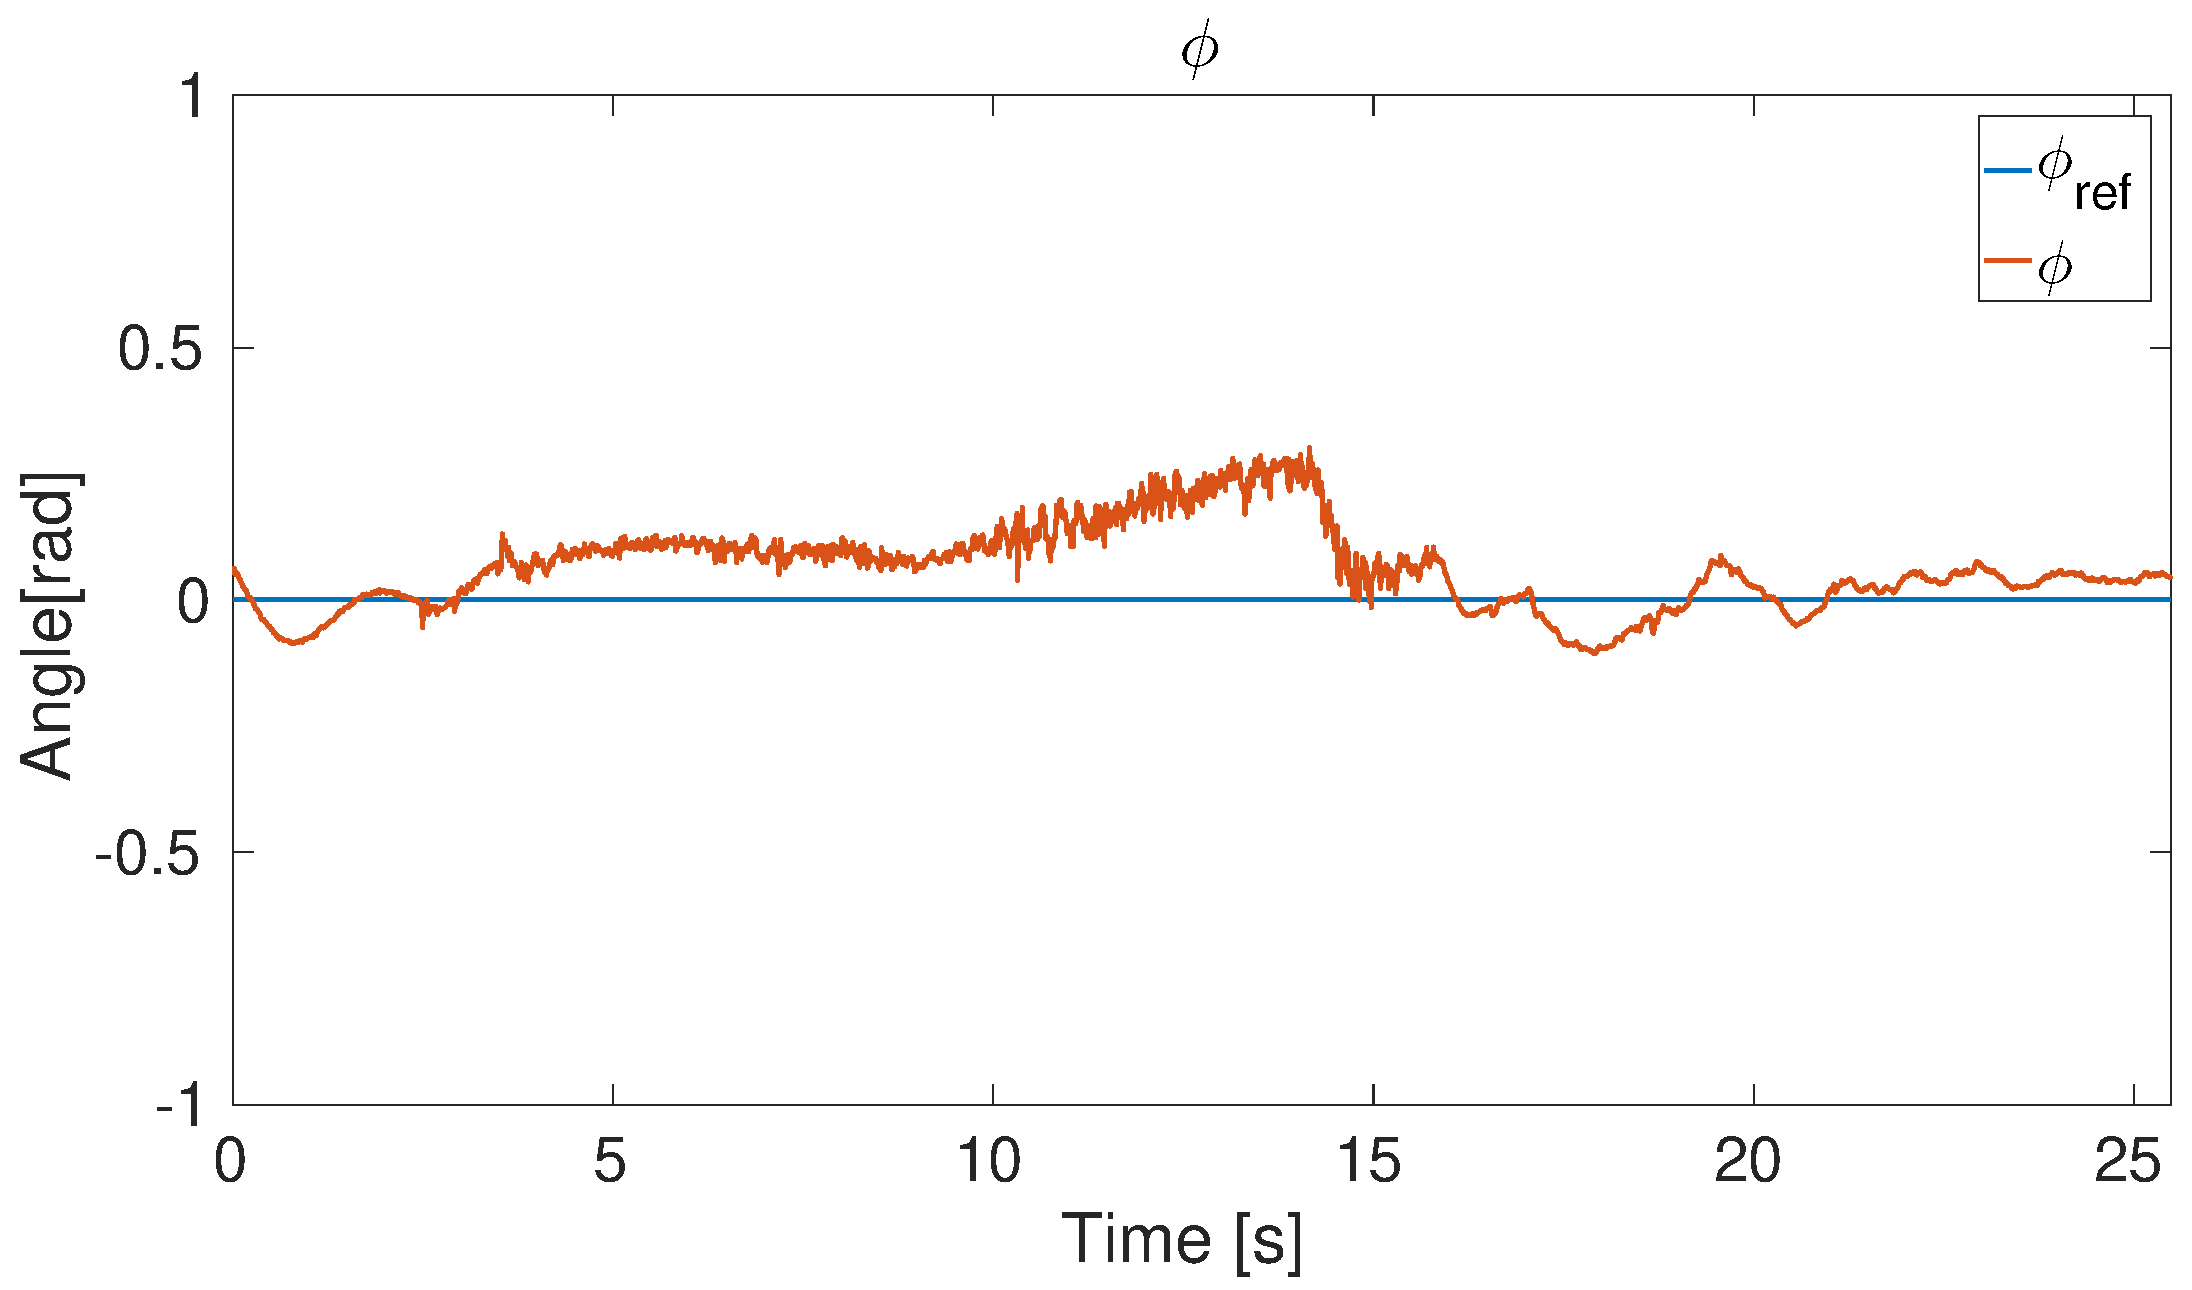
\includegraphics[width=0.4\textwidth]{testExactLinAttitudePhi}}
  \qquad
  \subfloat[][\label{fig:testExactAttitudePitch} The exact linearisation in $\pitchAngle$.]{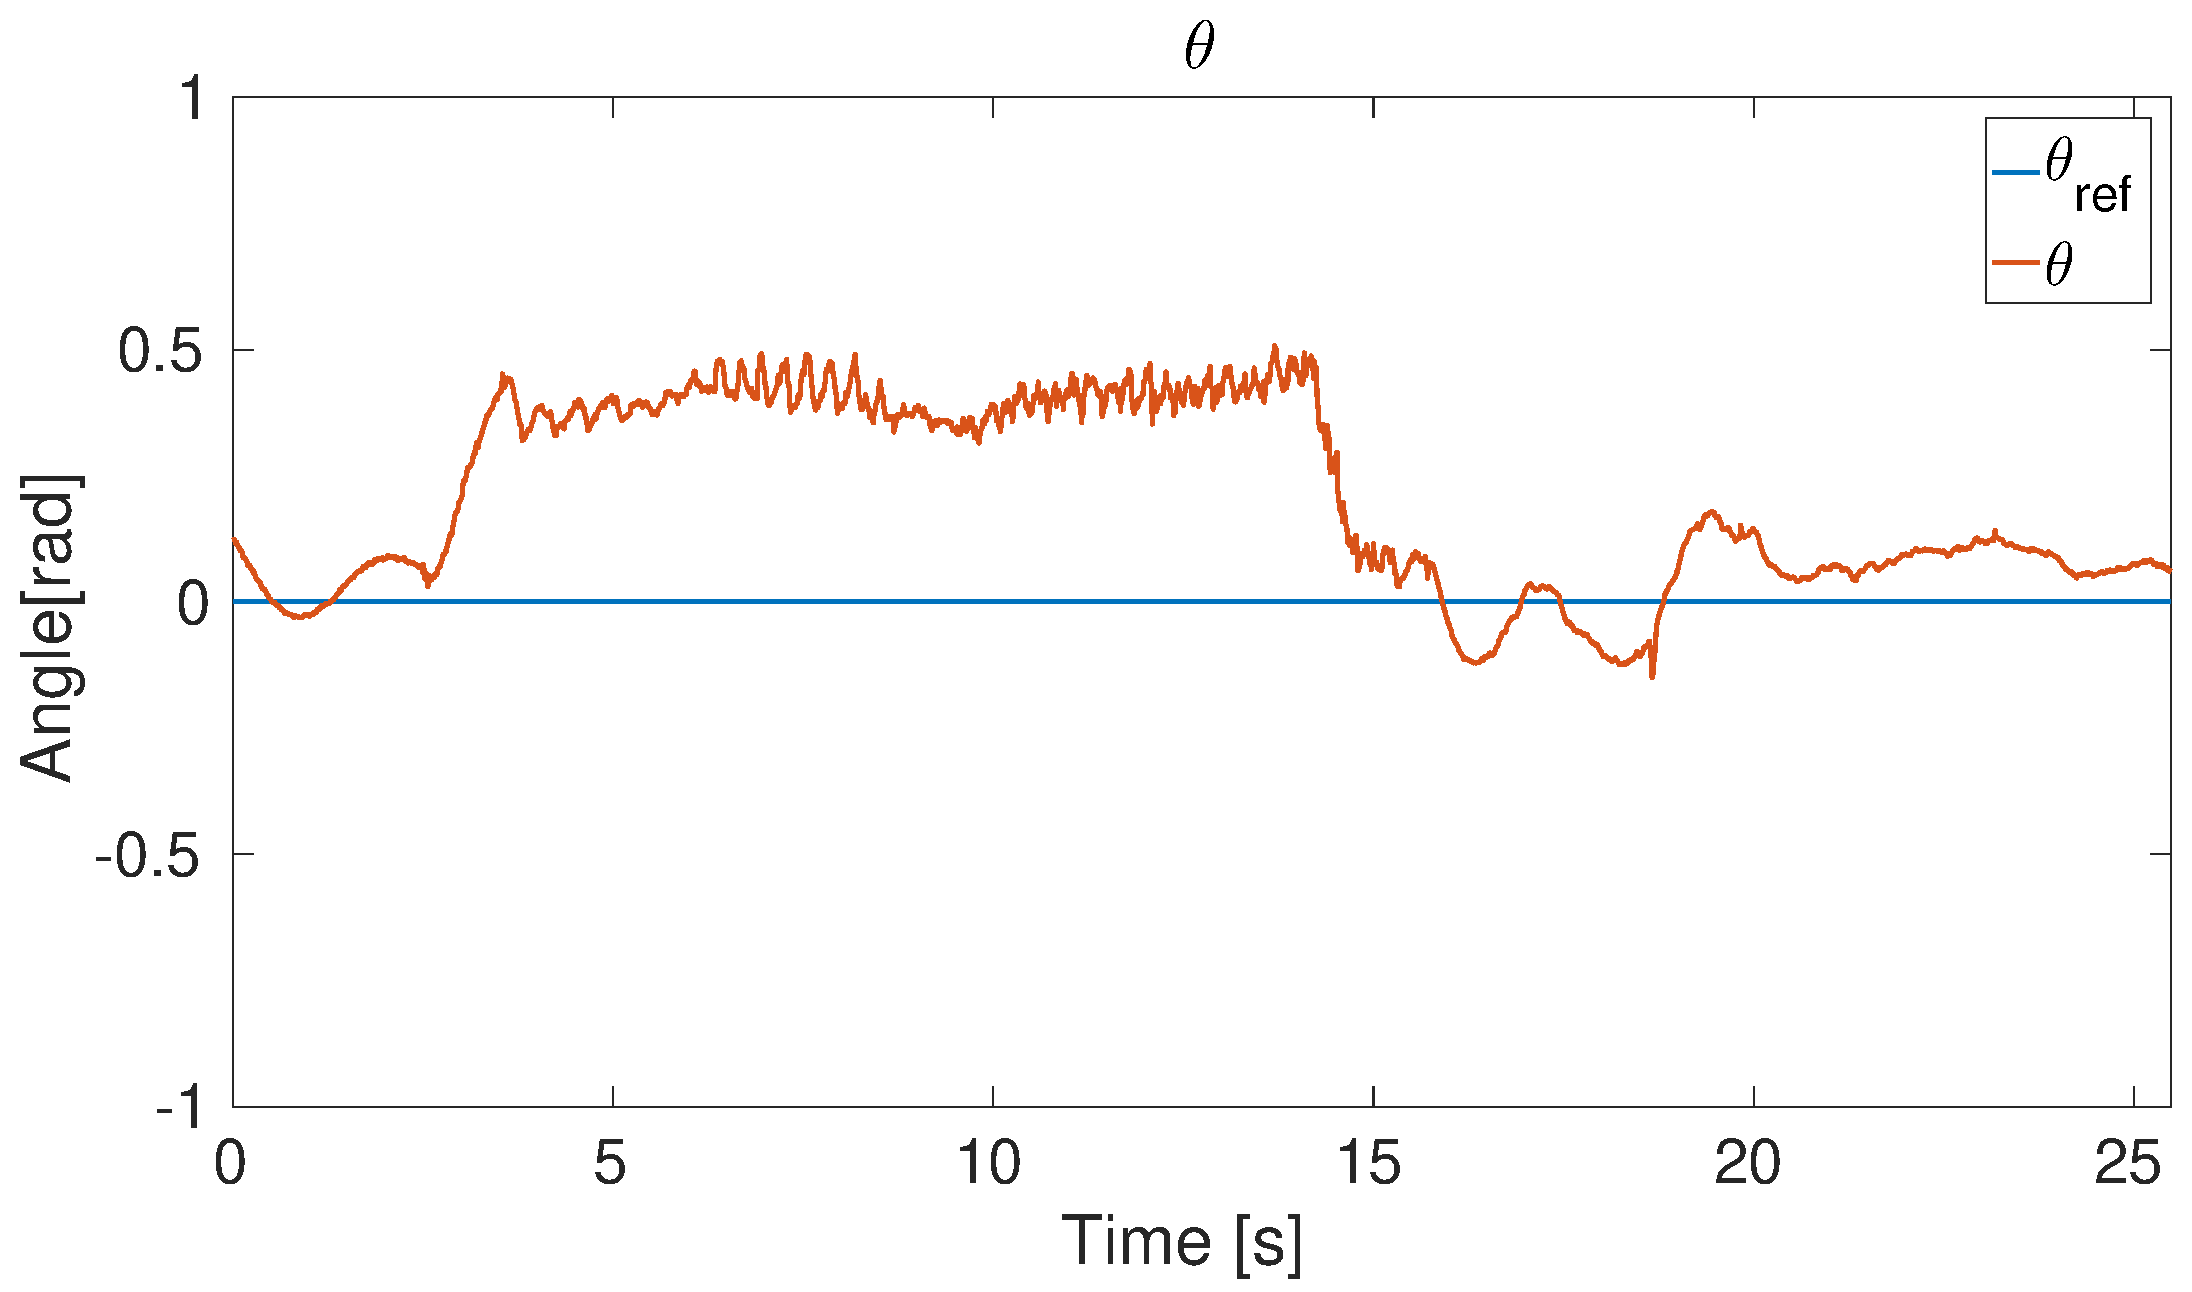
\includegraphics[width=0.4\textwidth]{testExactLinAttitudeTheta}}
  \qquad
  \subfloat[][\label{fig:testExactAttitudeYaw} The exact linearisation in $\yawAngle$.]{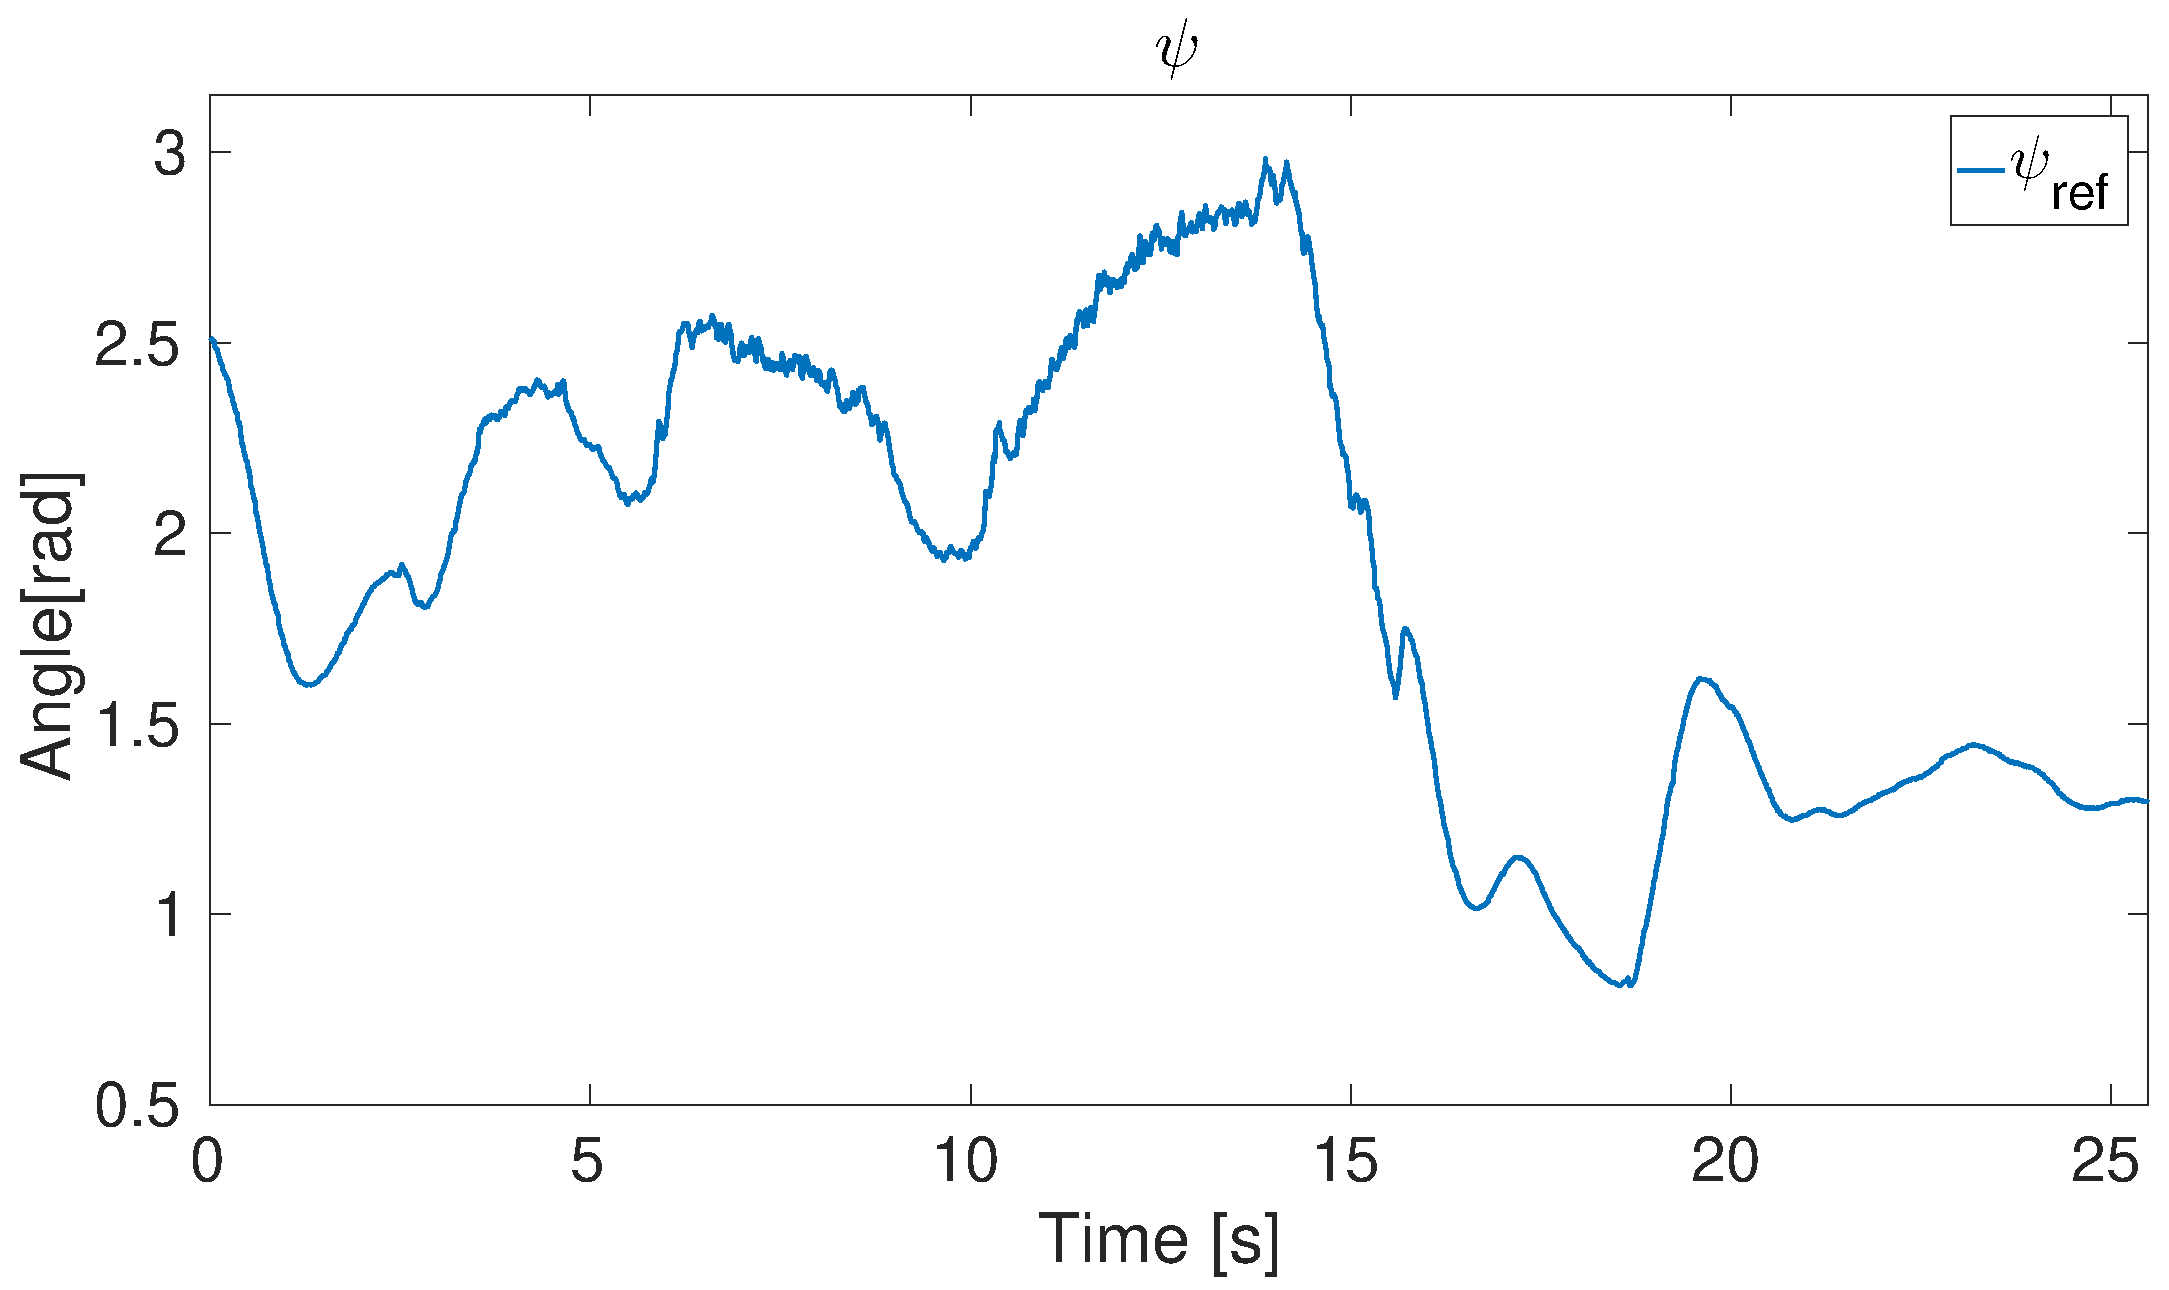
\includegraphics[width=0.4\textwidth]{testExactLinAttitudePsi}}
  \caption{\label{fig:ExactLinAttitude}% 
  The exact linearisation in the attitude controller. No reference signal was sent during this test thus is it only the effect of the exact linearisation showing.}
\end{figure}

\Figureref{fig:ExactLinAttitude} shows the exact linearisation in the attitude controller. Even that no reference signals are given begins the \abbrROV to change attitude.  
%%%%%%%%%%%%%%%%%%%%%%%%%%%Attitude%%%%%%%%%%%%%%%%%

\begin{figure}
\centering
  \subfloat[][\label{fig:testStepAllRollAttitude} A smooth step applied in $\rollAngle$.]{\includegraphics[width=0.4\textwidth]{testStepAllPhis3e10a1}}
  \qquad
  \subfloat[][\label{fig:simStepAllRollAttitude} A smooth step applied to the simulated \abbrROV in $\rollAngle$.]{\includegraphics[width=0.4\textwidth]{simStepAllPhis3e10a1}}
  \qquad
  \subfloat[][\label{fig:TestStepAllPitchAttitude} A smooth step applied in $\pitchAngle$.]{\includegraphics[width=0.4\textwidth]{testStepAllThetas3e10a1}}
  \qquad
  \subfloat[][\label{fig:simStepAllPitchAttitude} A smooth step applied to the simulated \abbrROV in $\pitchAngle$.]{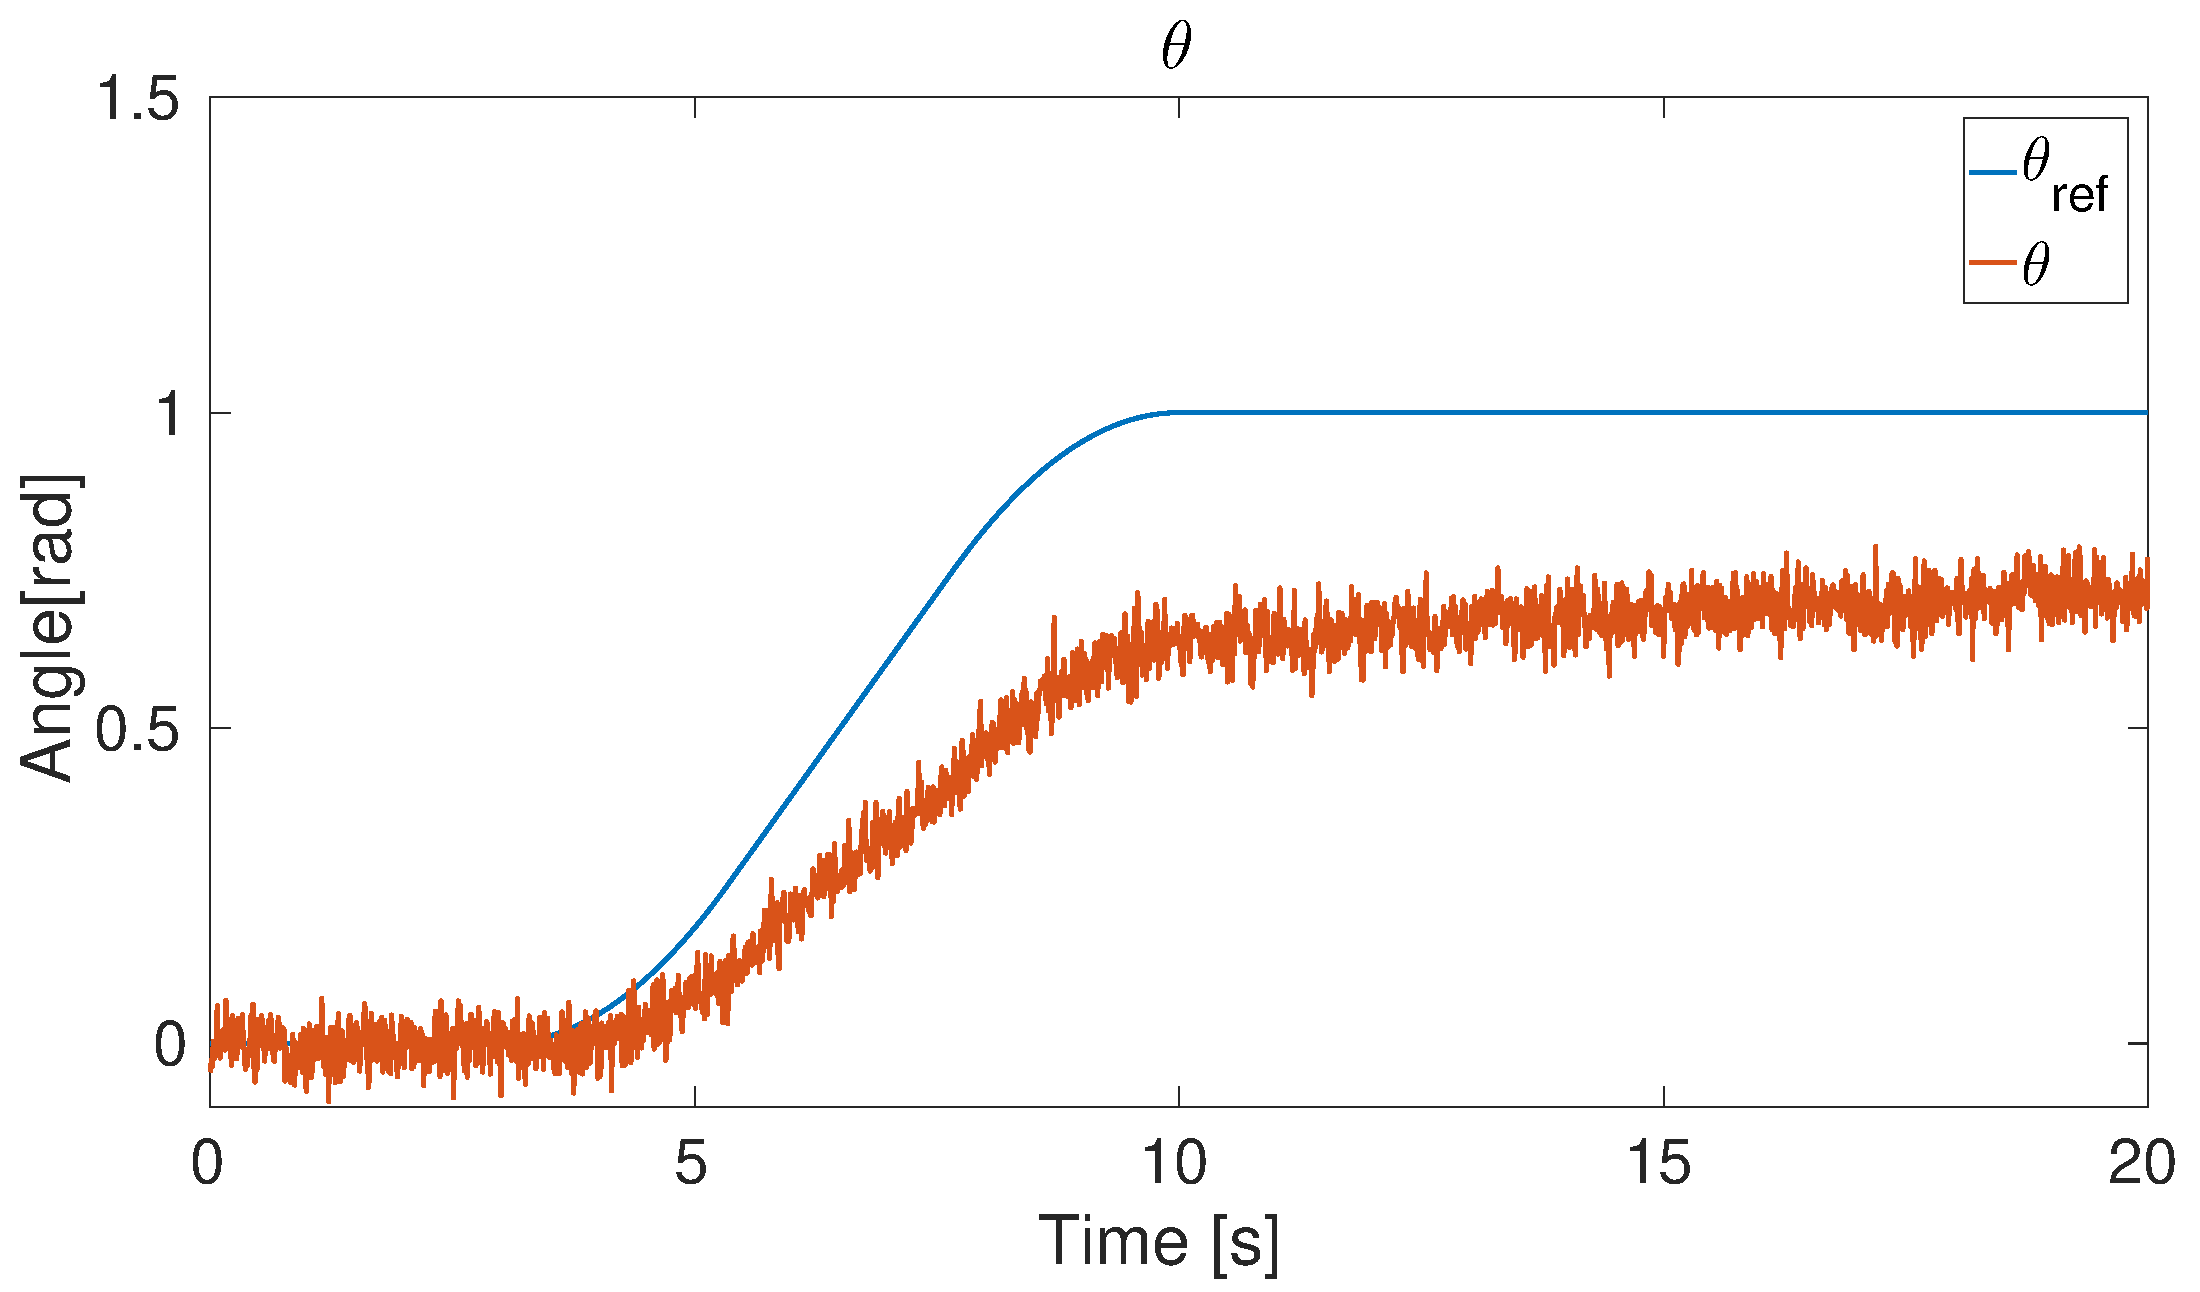
\includegraphics[width=0.4\textwidth]{simStepAllThetas3e10a1}}
  \qquad
  \subfloat[][\label{fig:TestStepAllYawAttitude} A smooth step applied in $\yawAngle$.]{\includegraphics[width=0.4\textwidth]{testStepAllPsis3e10a1}}
  \qquad
  \subfloat[][\label{fig:simStepAllYawAttitude} A smooth step applied to the simulated \abbrROV in $\yawAngle$.]{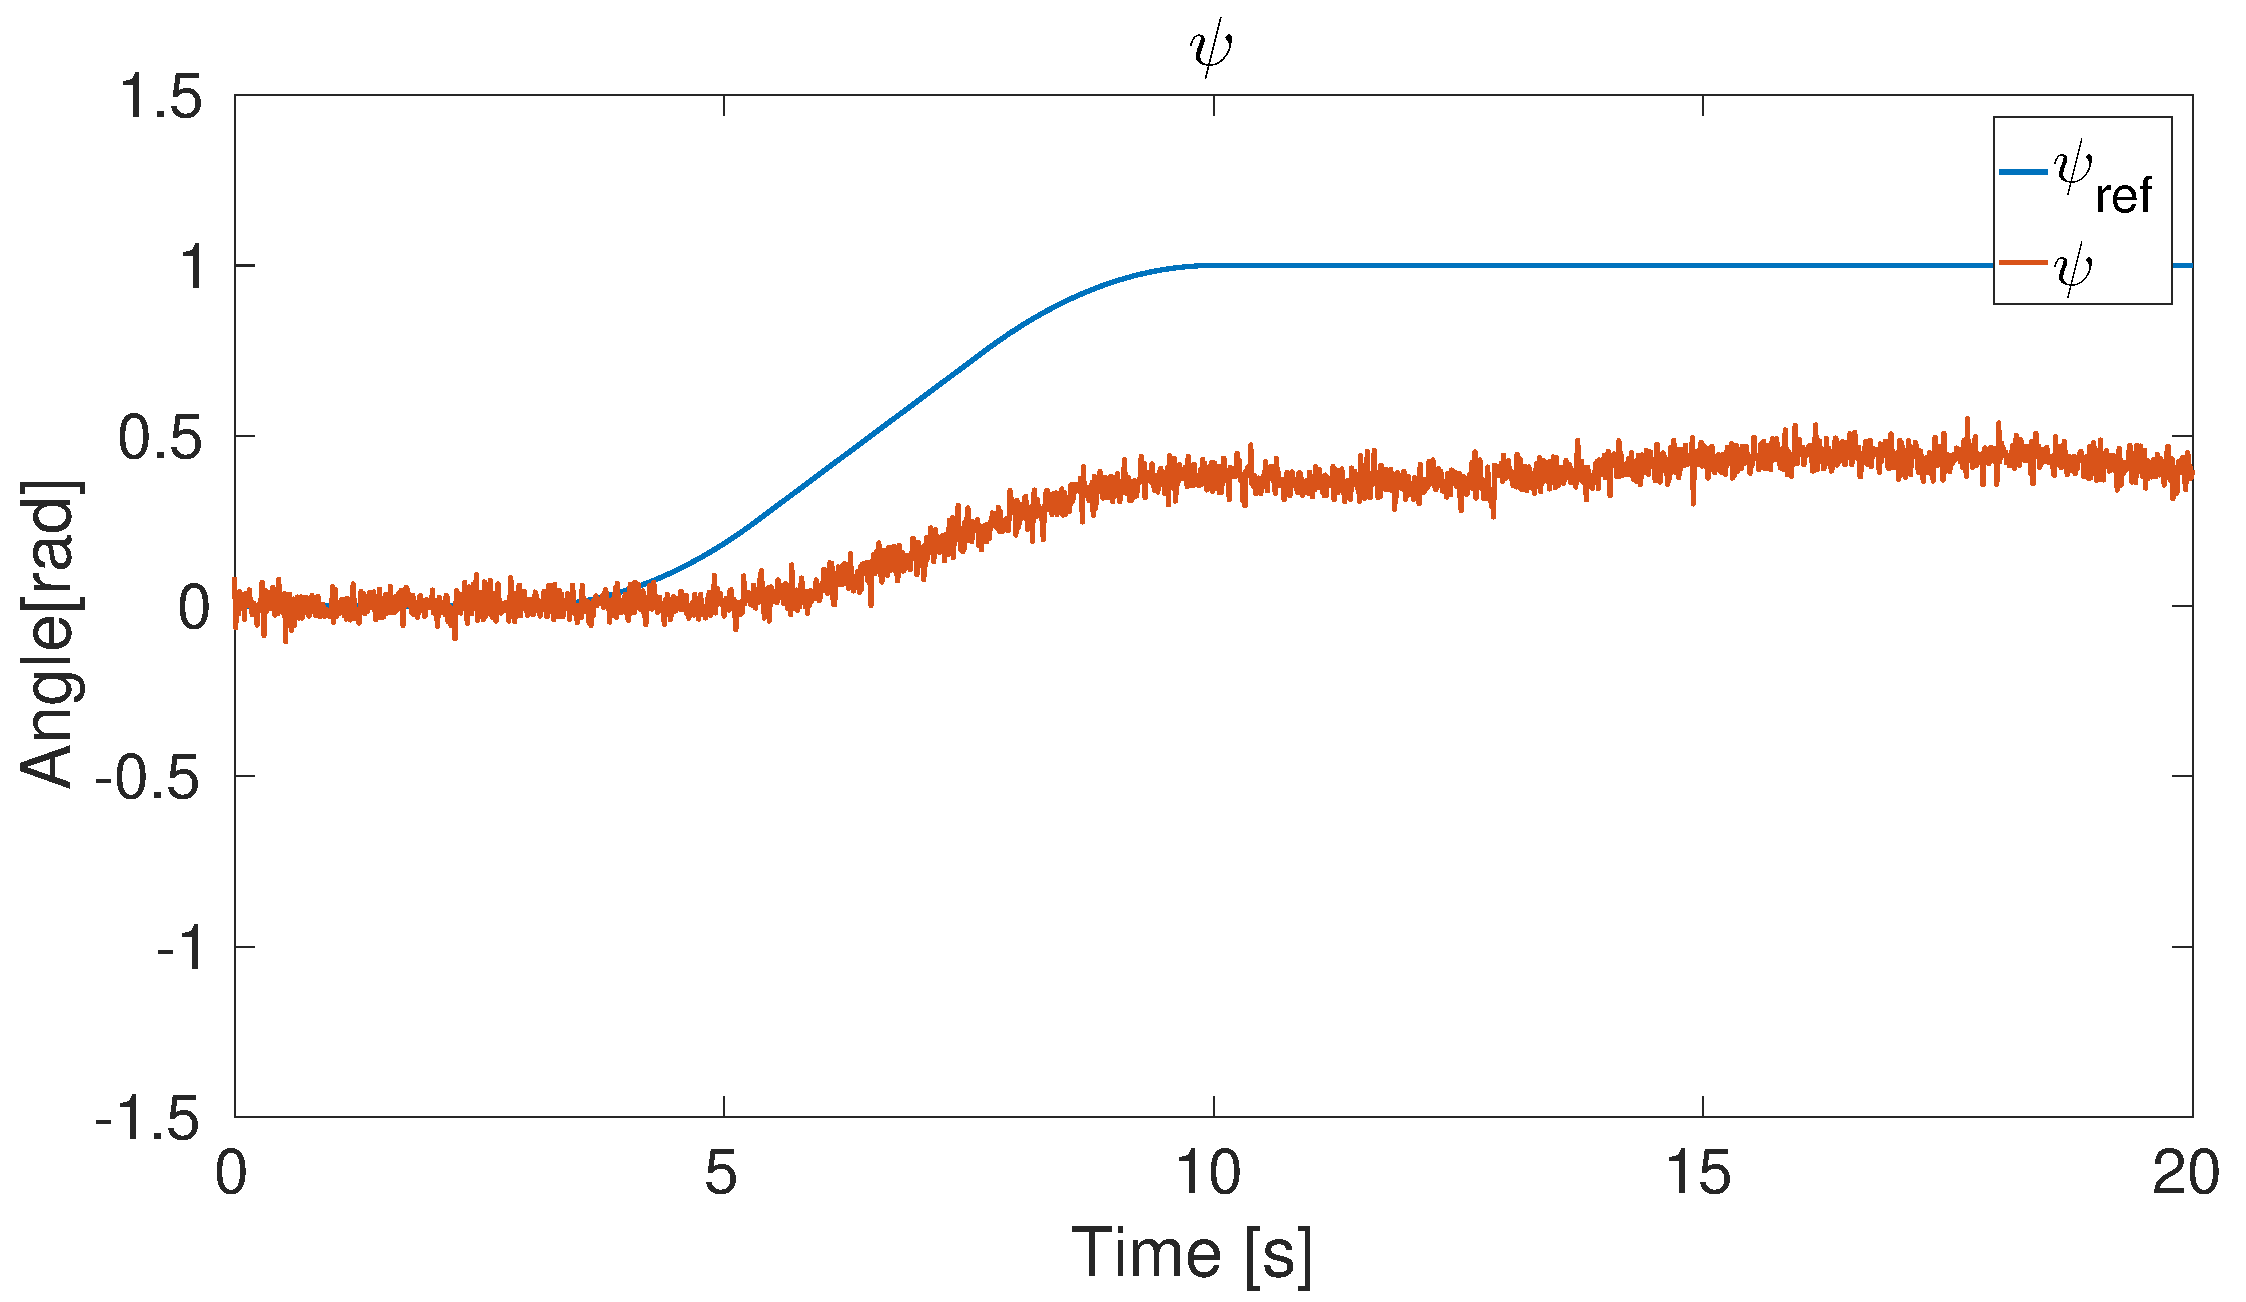
\includegraphics[width=0.4\textwidth]{simStepAllPsis3e10a1}}
  \caption{\label{fig:StepAllAttitude}% 
  Smooth steps were applied in all attitude angles at the same time while using the attitude controller.}
\end{figure}

\Figureref{fig:StepAllAttitude} shows smooth step reference signals applied in all attitude angles while using the attitude controller. Initially did $\rollAngle$ and $\pitchAngle$ follow the reference signals well in the real test. The $\rollAngle$ oscillated with a steady state error of 0.9 in the real test. However, $\pitchAngle$ was kept closer to the reference signal with a steady state error of 0.4. The attitude angle $\yawAngle$ could not be stabilised during the real test and drifted throughout the test. In the simulated test case did not the attitude angles reach the reference signal. The attitude angle $\pitchAngle$ had a steady state error of 0.3 and the other angles had a steady state error of 0.5.

\begin{figure}
\centering
  \subfloat[][\label{fig:testSinAllRollAttitude} A sine signal with amplitude $1$ and frequency $0.5\hertz$ applied in $\rollAngle$.]{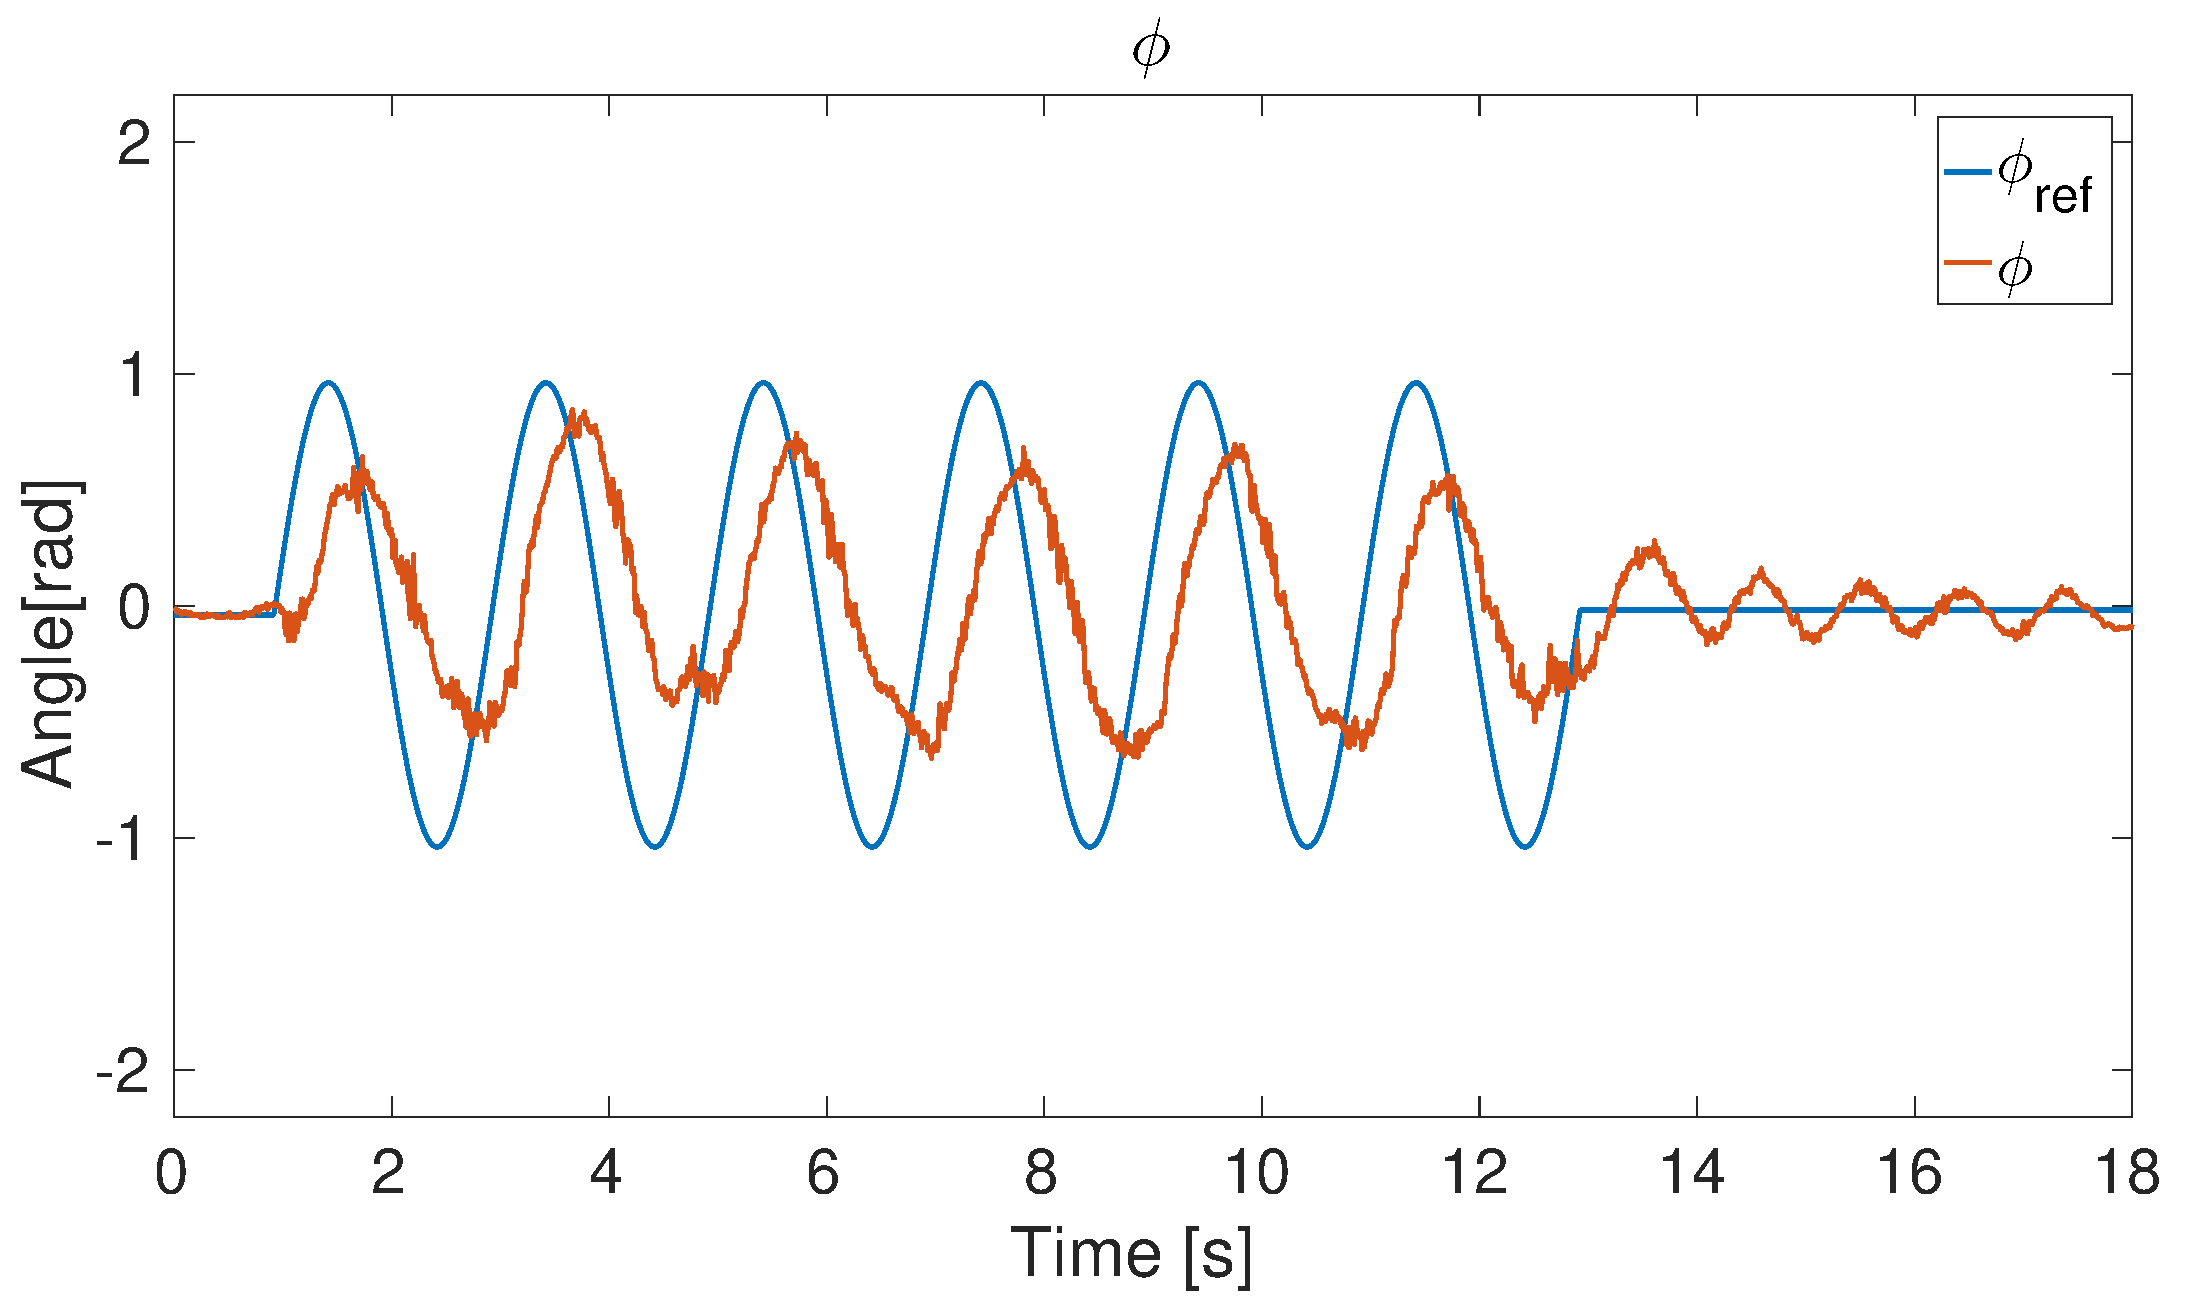
\includegraphics[width=0.4\textwidth]{testSinAllPhiA1}}
  \qquad
  \subfloat[][\label{fig:simSinAllRollAttitude} A sine signal with amplitude $1$ and frequency $0.5\hertz$ applied to the simulated \abbrROV in $\rollAngle$.]{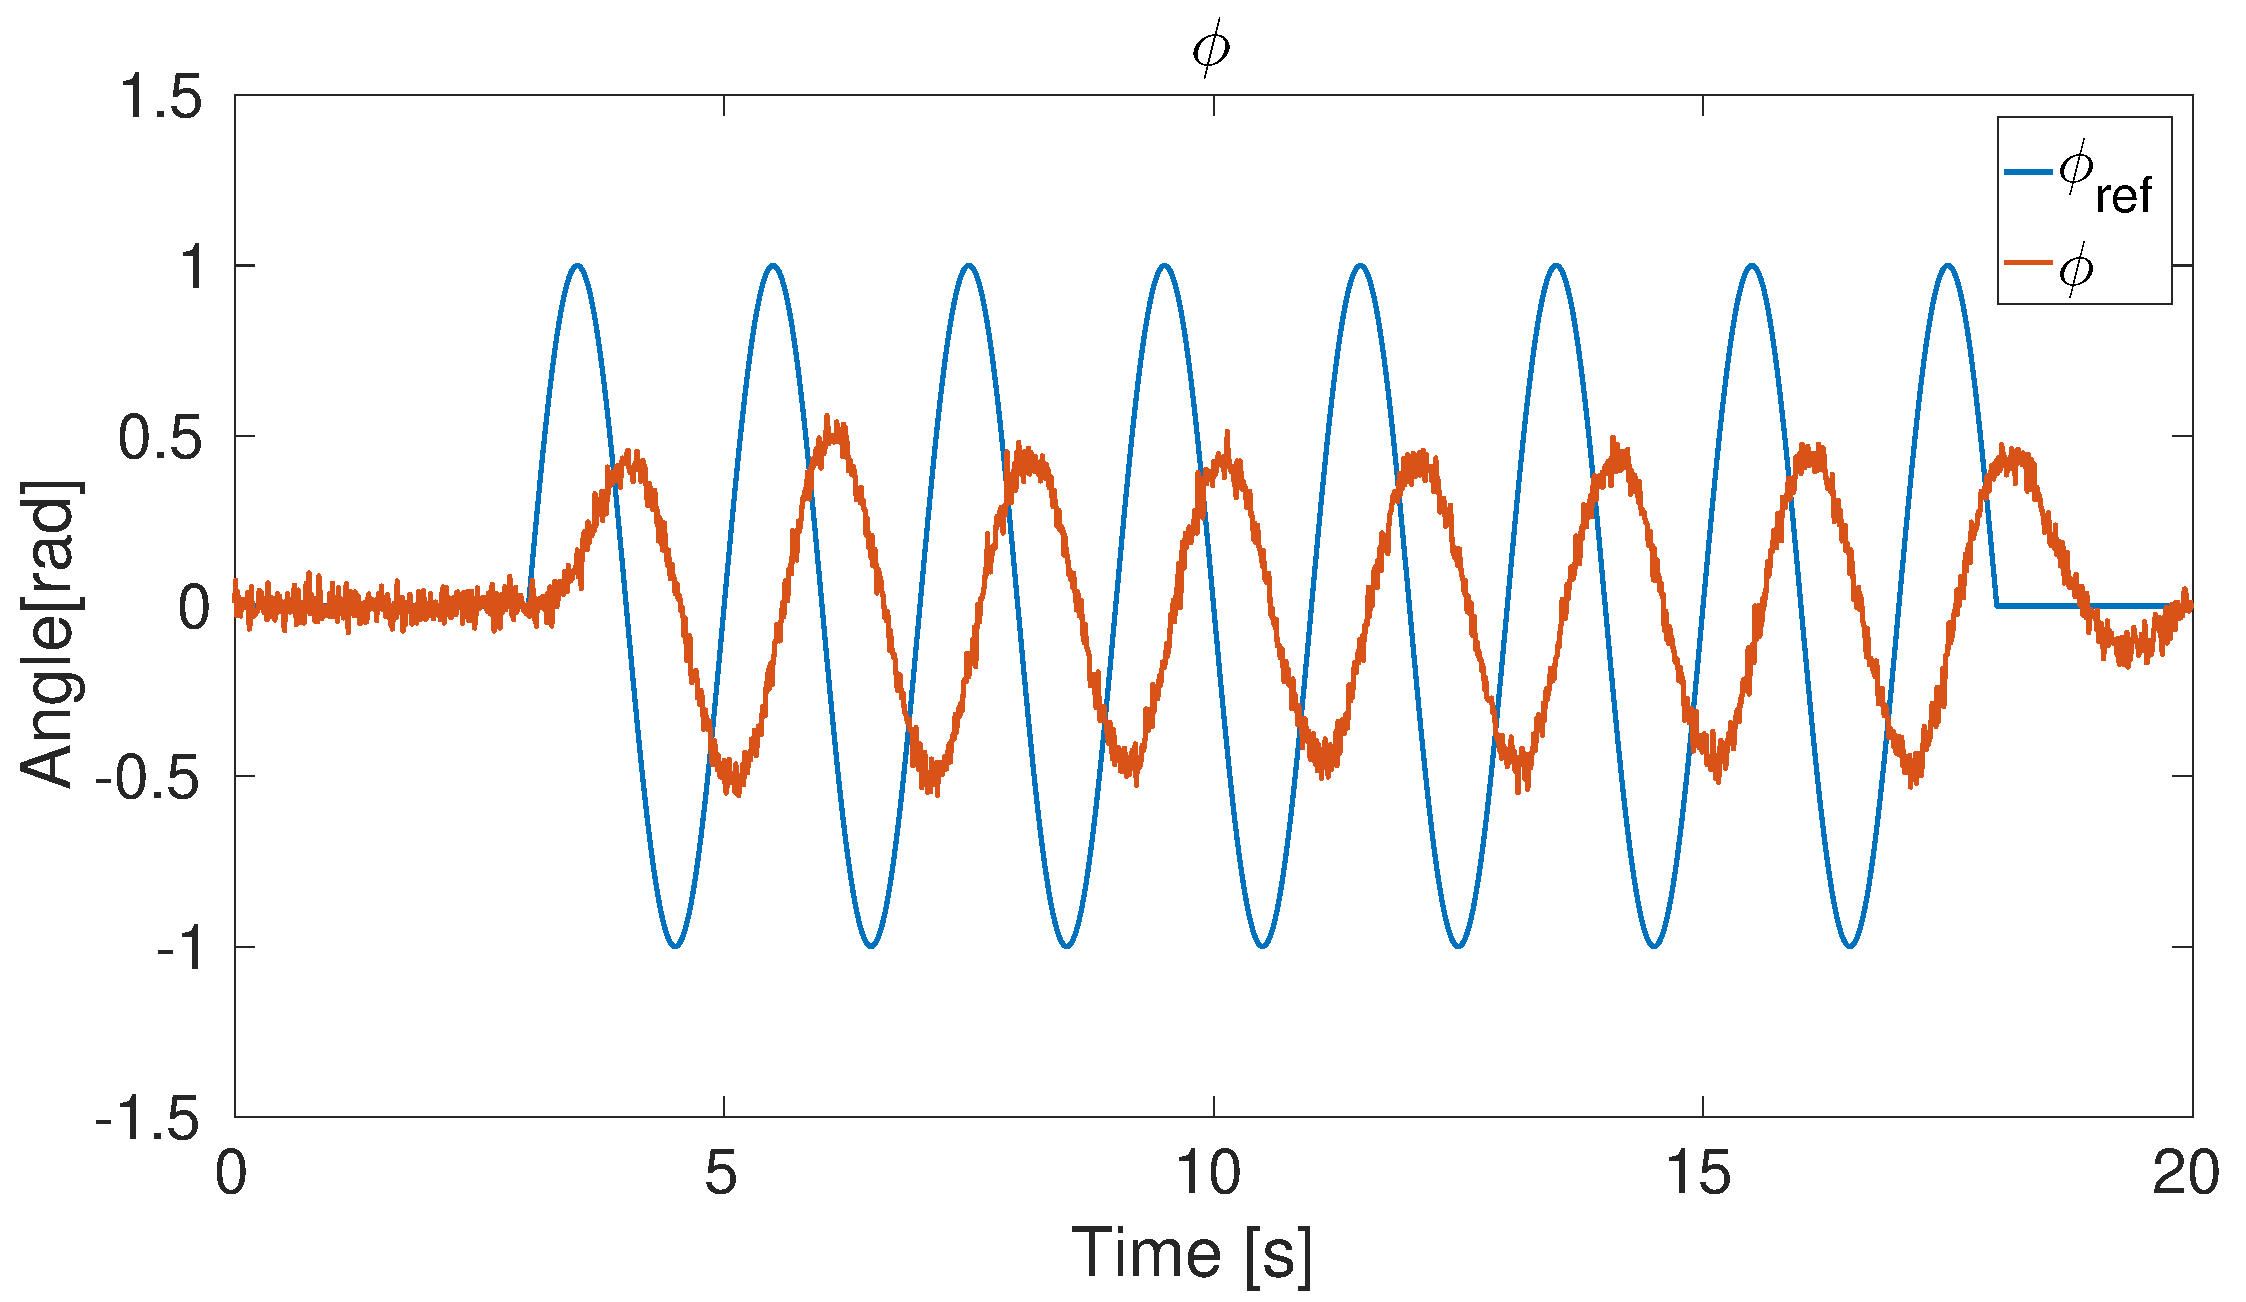
\includegraphics[width=0.4\textwidth]{simSinAllPhiA1}}
  \qquad
  \subfloat[][\label{fig:testSinAllPitchAttitude} A sine signal with amplitude $1$ and frequency $0.5\hertz$ applied in $\pitchAngle$.]{\includegraphics[width=0.4\textwidth]{testSinAllThetaA1}}
  \qquad
  \subfloat[][\label{fig:simSinAllPitchAttitude} A sine signal with amplitude $1$ and frequency $0.5\hertz$ applied to the simulated \abbrROV in $\pitchAngle$.]{\includegraphics[width=0.4\textwidth]{simSinAllThetaA1}}
  \qquad
  \subfloat[][\label{fig:testSinAllYawAttitude} A sine signal with amplitude $1$ and frequency $0.5\hertz$ applied in $\yawAngle$.]{\includegraphics[width=0.4\textwidth]{testSinAllPsiA1}}
  \qquad
  \subfloat[][\label{fig:simSinAllYawAttitude} A sine signal with amplitude $1$ and frequency $0.5\hertz$ applied to the simulated \abbrROV in $\yawAngle$.]{\includegraphics[width=0.4\textwidth]{simSinAllPsiA1}}
  \caption{\label{fig:SinAllAttitude}%
  Sine signals were applied in all attitude angles at the same time while using the attitude controller.}
\end{figure}

Sine reference signals with amplitude 1 and frequency $0.5 \hertz$ can be seen in \Figureref{fig:SinAllAttitude}. The angles $\rollAngle$ and $\pitchAngle$ did not reached the assigned amplitude in the real test. However, did they have the general form of a sine but phase shifted relative to the reference signals. The $\yawAngle$ follows the reference signal well but with a phase shift and a bias. In simulation tests the same phase shift and lack of amplitude happened in $\rollAngle$ and $\pitchAngle$. The simulated result in $\yawAngle$ did not follow the reference signal at all. 

\begin{figure}
\centering
  \subfloat[][\label{fig:testStepPhiTheta05RollAttitude} A smooth step applied in $\rollAngle$.]{\includegraphics[width=0.4\textwidth]{testStepThetaPhiPhis3e10a1}}
  \qquad
  \subfloat[][\label{fig:simStepPhiTheta05RollAttitude} A smooth step applied to the simulated \abbrROV in $\rollAngle$.]{\includegraphics[width=0.4\textwidth]{simStepThetaPhiPhis3e10a1}}
  \qquad
  \subfloat[][\label{fig:testStepPhiTheta05PitchAttitude} A smooth step applied in $\pitchAngle$.]{\includegraphics[width=0.4\textwidth]{testStepThetaPhiThetas3e10a1}}
  \qquad
  \subfloat[][\label{fig:simStepPhiTheta05PitchAttitude} A smooth step applied to the simulated \abbrROV in $\pitchAngle$.]{\includegraphics[width=0.4\textwidth]{simStepThetaPhiThetas3e10a1}}
  \caption{\label{fig:StepPhiThetaAttitude}%
  Smooth steps were applied in \pitchAngle and \rollAngle at the same time while using the attitude controller. The attitude angle $\yawAngle$ was kept free during the test.}
\end{figure}

A smoothed step in $\rollAngle$ and $\pitchAngle$ can be seen in \Figureref{fig:StepPhiThetaAttitude}. During the test was the attitude angle $\yawAngle$ kept free. Both $\rollAngle$ and $\pitchAngle$ followed the reference signal well did not reach the reference angle. The steady state error for $\rollAngle$ and $\pitchAngle$ was approximately $0.35$. The simulated results in $\rollAngle$ and $\pitchAngle$ were worse than the real test. The attitude $\rollAngle$ had a steady state error 0.5 and the steady state error for $\pitchAngle$ was 0.4.

%%%%%%%%%%%%%%%%%%%%%%%%%%%Rate%%%%%%%%%%%%%%%%
\begin{figure}
\centering
  \subfloat[][\label{fig:testStepAllPRate} A smooth step applied in $\rollVelocity$.]{\includegraphics[width=0.4\textwidth]{testStepAllPs3e10a1}}
  \qquad
  \subfloat[][\label{fig:simStepAllPRate} A step applied to the simulated \abbrROV in $\rollVelocity$.]{\includegraphics[width=0.4\textwidth]{simStepAllPs3e10a1}}
  \qquad
  \subfloat[][\label{fig:testStepAllQRate} A smooth step applied in $\pitchVelocity$.]{\includegraphics[width=0.4\textwidth]{testStepAllQs3e10a1}}
  \qquad
  \subfloat[][\label{fig:simStepAllQRate} A step applied to the simulated \abbrROV in $\pitchVelocity$.]{\includegraphics[width=0.4\textwidth]{simStepAllQs3e10a1}}
  \qquad
  \subfloat[][\label{fig:testStepAllRRate} A smooth step applied in $\yawVelocity$.]{\includegraphics[width=0.4\textwidth]{testStepAllRs3e10a1}}
  \qquad
  \subfloat[][\label{fig:simStepAllRRate} A step applied to the simulated \abbrROV in $\yawVelocity$.]{\includegraphics[width=0.4\textwidth]{simStepAllRs3e10a1}}
  \caption{\label{fig:StepAllRate}% 
  Smooth steps were applied in all angular velocities at the same time while using the rate controller.}
\end{figure}

\Figureref{fig:StepAllRate} shows a smooth step applied in all angular velocities while using the rate controller. An overshoot of 0.5 is achieved in $\rollVelocity$ for the real test while in the simulation only has an overshoot of 0.2. Both the real test and the simulation in $\rollVelocity$ followed the reference signal well and had a small steady state error. The real and simulated test followed the reference value well in $\pitchVelocity$ and had negligible steady state errors. However, had the real test no overshoot while the simulation in $\pitchVelocity$ had an overshoot of 0.4. The simulated test in $\yawVelocity$ performed really well and almost followed the reference perfectly. The real test in $\yawVelocity$ performed well, but it was slow to rise to the requested reference signal and had a small steady state error of 0.1. 

\begin{figure}
\centering
  \subfloat[][\label{fig:testSinAllPRate} A sine signal with amplitude $1$ and frequency $0.5\hertz$ applied in $\rollVelocity$.]{\includegraphics[width=0.4\textwidth]{testSinAllPA1}}
  \qquad
  \subfloat[][\label{fig:simSinAllPRate}A sine signal with amplitude $1$ and frequency $0.5\hertz$ applied to the simulated \abbrROV in $\rollVelocity$.]{\includegraphics[width=0.4\textwidth]{simSinAllPA1}}
  \qquad
  \subfloat[][\label{fig:testSinAllQRate} A sine signal with amplitude $1$ and frequency $0.5\hertz$ applied in $\pitchVelocity$.]{\includegraphics[width=0.4\textwidth]{testSinAllQA1}}
  \qquad
  \subfloat[][\label{fig:simSinAllQRate} A sine signal with amplitude $1$ and frequency $0.5\hertz$ applied to the simulated \abbrROV in $\pitchVelocity$.]{\includegraphics[width=0.4\textwidth]{simSinAllQA1}}
  \qquad
  \subfloat[][\label{fig:testSinAllRRate} A sine signal with amplitude $1$ and frequency $0.5\hertz$ applied in $\yawVelocity$.]{\includegraphics[width=0.4\textwidth]{testSinAllRA1}}
  \qquad
  \subfloat[][\label{fig:simSinAllRRate} A sine signal with amplitude $1$ and frequency $0.5\hertz$ applied to the simulated \abbrROV in $\yawVelocity$.]{\includegraphics[width=0.4\textwidth]{simSinAllRA1}}
  \caption{\label{fig:SinAllRate}%
  Sine signals were applied in all angular velocities at the same time while using the rate controller.}
\end{figure}

Sine signals were applied to all angular velocities which can be seen in \Figureref{fig:SinAllRate} while using the rate controller. In the real test followed all the angular velocities the reference signals well, except for some overshoots and undershoots of the requested amplitude. The simulated test followed a general sine form but the reference amplitude was not reach and a phase shift could be noted.

%%%%%%%%%%%%%%%%%%%%%%%%%%%Depth%%%%%%%%%%%%%%%%
\begin{figure}[tbp]
  \centering
  \subfloat[][\label{fig:testStepD1} A smooth step applied in $\zPosition$.]{\includegraphics[width=0.4\textwidth]{testStepDepth3e10a1}}
  \qquad
  \subfloat[][\label{fig:testStepD2} A step applied in $\zPosition$.]{\includegraphics[width=0.4\textwidth]{testConstantD1}}
  \caption{\label{fig:StepD}%
    Steps applied to $\zPosition$. A smooth step from $0.4 \meter$ to $1 \meter$ is shown in (a) and a step from $0.5 \meter$ to $2 \meter$ is shown in (b).}
\end{figure}

\Figureref{fig:StepD} shows a smooth step from $0.4 \meter$ to $1 \meter$ and a step from $0.5 \meter$ to $2 \meter$. A delay in the response can be seen and overshoots of approximately 0.2.

%%%%%%%%%%%%%%%%%%%%%%%%%%%%%%%%%%%%%%%%
\section{Discussion}


\chapter{Conclusions}\label{cha:conclusions}


\section{Future Work}


\part*{Appendix}
\appendix
\chapter{Dependencies and Installation}\label{app:dependencies}
The following dependencies are some of the needed packages for compiling and running the \abbrROV.
\begin{itemize}
    \item Ubuntu 14.04
    \item ROS Indigo Igloo
    \item rosserial (Indigo)
    \item rosserial\_arduino (Indigo)
    \item image\_common (Indigo) 
    \item image\_transport (Indigo)
    \item joy (Indigo)
\end{itemize}

More details of the necessary packages are listed in the installation guide.

%%%%%%%%%%%%%%%%%%%%%%%%%%%%%%%%%%%%%%%%%%%%%%%%%%%%%%%%%%%%%%%%%%%%%%%%%%%%%%%%%%%
\section{Raspberry Pi installation}
This section summarises how to setup the Raspberry Pi. It is assumed that the Raspberry Pi is already running Ubuntu 14.04.

\subsection{\abbrROS Installation}
To install \abbrROS the \abbrROS source needs to be in the source listing run

\begin{lstlisting}[language=bash]
sudo sh -c 'echo "deb http://packages.ros.org/ros/ubuntu $(lsb_release -sc) main" > /etc/apt/sources.list.d/ros-latest.list' && sudo apt-get install ros-indigo-ros-base -y && sudo rosdep init && rosdep update && echo "source /opt/ros/indigo/setup.bash" >> ~/.bashrc && source ~/.bashrc && sudo apt-get upgrade -y && sudo ln -s /usr /opt/vc
\end{lstlisting}
to install \abbrROS and source the necessary files.

The packages needed and some other packages used in the \abbrROV is installed by
\begin{lstlisting}[language=bash]
sudo apt-get install libraspberrypi-bin libraspberrypi-dev openssh-server build-essential avahi-daemon linux-firmware python-rosinstall ros-indigo-rosserial ros-indigo-rosserial-arduino ros-indigo-image-common ros-indigo-image-transport-plugins git && sudo sh -c 'echo "start_x=1\ngpu_mem=128" >> /boot/config.txt'
\end{lstlisting}
then restart the Raspberry pi.

\subsection{Tether Setup}
For communication with the workstation the hostnames and Ethernet port needs to be setup.
Configure the host file 
\begin{lstlisting}
sudo nano /etc/hosts
\end{lstlisting}
add
\begin{lstlisting}
10.0.0.20 bluerov
10.0.0.10 workstation
\end{lstlisting}
to the host file. To use a static IP for the \abbrROV configure the interfaces file
\begin{lstlisting}
sudo nano /etc/network/interfaces
\end{lstlisting}
add 
\begin{lstlisting}
auto eth0
iface eth0 inet static
    address 10.0.0.20
    netmask 255.255.255.0
\end{lstlisting}
to the interfaces file. Reboot the computer or restart the networking services for changes to take effect.

\subsection{Installation of the \abbrROV package}
To download and to compile the package run
\begin{lstlisting}
git clone https://github.com/MrEkelund/ExjobbROV.git && cd ExjobbROV/catkin_ws && catkin_make && echo "source ~/path-to-package/ExjobbROV/catkin_ws/devel/setup.bash" >> ~/.bashrc 
\end{lstlisting}

Setup the communication with the arduino.
\begin{lstlisting}
sudo cp ExjobbROV/catkin_ws/src/bluerov/extra/99-bluerov.rules /etc/udev/rules.d/ && sudo udevadm trigger
\end{lstlisting}

Compile the arduino code and flash it to the arduino by running
\begin{lstlisting}
cd ExjobbROV/catkin_ws && catkin_make bluerov_arduino_firmware && catkin_make bluerov_arduino_firmware-upload
\end{lstlisting}

%%%%%%%%%%%%%%%%%%%%%%%%%%%%%%%%%%%%%%%%%%%%%%%%%%%%%%%%%%%%%%%%%%%%%%%%%%%%%%%%%%%
\section{Workstation Installation}
This section summarises how to setup the workstation for operation with the \abbrROV. It's assumed that the workstation is already running Ubuntu 14.04. 

\subsection{\abbrROS Installation}
To install \abbrROS run the following command
\begin{lstlisting}[language=bash]
sudo sh -c 'echo "deb http://packages.ros.org/ros/ubuntu $(lsb_release -sc) main" > /etc/apt/sources.list.d/ros-latest.list' && sudo apt-get install ros-indigo-ros-desktop-full && sudo rosdep init && rosdep update && echo "source /opt/ros/indigo/setup.bash" >> ~/.bashrc && source ~/.bashrc
\end{lstlisting}
then run 
\begin{lstlisting}
sudo apt-get install python-rosinstall ros-indigo-rosserial ros-indigo-rosserial-arduino ros-indigo-image-common ros-indigo-image-transport-plugins ros-indigo-joy sshpass git
\end{lstlisting}
to install some necessary packages.

\subsection{Tether Setup}
For communication with the \abbrROV the hostnames and Ethernet port needs to be setup.
Configure the host file 
\begin{lstlisting}
sudo nano /etc/hosts
\end{lstlisting}
add
\begin{lstlisting}
10.0.0.20 bluerov
10.0.0.10 workstation
\end{lstlisting}
to the host file. To use a static IP for the workstation configure the interfaces file
\begin{lstlisting}
sudo nano /etc/network/interfaces
\end{lstlisting}
add 
\begin{lstlisting}
auto eth0
iface eth0 inet static
    address 10.0.0.10
    netmask 255.255.255.0
\end{lstlisting}
to the interfaces file. Reboot the computer or restart the networking services for changes to take effect. The static IP can also be set in the network configuration GUI for Ubuntu.

\subsection{Installation of the \abbrROV package}
To download and to compile the package run
\begin{lstlisting}
git clone https://github.com/MrEkelund/ExjobbROV.git && cd ExjobbROV/catkin_ws && catkin_make
\end{lstlisting}
\chapter{Operation of the \abbrROV} \label{app:operation}

\section{Start up of the \abbrROV}
For starting the \abbrROV connect all cables according to \ref{sec:}.
\begin{itemize}
	\item Make sure that the battery is tightly fastened and is fully charged. 
	\item Slide the cradle gently into the \abbrROV tube. 
	\item If needed apply some silicone grease to the O-rings of the end cap. Then slide the end cap into the \abbrROV tube.
	\item Insert the vent bolt in to the vent nut on the end cap.
	\item Insert the cat 6 cable to the workstation.
 \end{itemize} 
Navigate to the catkin\_ws folder on the workstation and run the start script in a terminal for the \abbrROV
\begin{lstlisting}
 ./startrov.sh
\end{lstlisting}
Then in a new terminal navigate to the catkin\_ws folder and run the workstation script
\begin{lstlisting}
 ./startworkstation.sh
\end{lstlisting} 
%%%%%%%%%%%%%%%%%%%%%%%%%%%%%%%%%%%%%%%%%%%%%%%%
\section{Operating the ROV}

\subsection{Modes and controllers}

\subsubsection{Manual mode}

\subsection{Logging data}
For logging of data rqt-bag is used. In rqt on the workstation start rqt-bag by Plugins $\rightarrow$ Logging $\rightarrow$ Bag. Start the recording of data by pressing the red circle. A menu of available topics is showed, select the topics that you want to record. Then give the logfile a name in the pop-up.
To stop recording data press the red circle and close Bag by Running $\rightarrow$ Close:Bag.

\subsection{Sending test signals}


\subsection{Displaying the continuous plots}


%%%%%%%%%%%%%%%%%%%%%%%%%%%%%%%%%%%%%%%%%%%%%%%%
\section{New Parameter Estimation and Controllers}
\subsection{Parameter Estimation}


\subsection{Code Generation of the Controller Node}


%%%%%%%%%%%%%%%%%%%%%%%%%%%%%%%%%%%%%%%%%%%%%%%%
\section{Known issues and troubleshooting}

\subsection{\abbrROS debugging}

\subsection{Check Ethernet connection}

\subsection{One or several thrusters are unresponsive}

\subsection{Checking and changing polarity of thrusters}

\chapter{Thruster mapping}\label{app:thrustmapping}

\VerbatimInput{sections/measuredthrust.txt}

\chapter{Controller Test Results}\label{app:controllerTestResults}
\todo[inline]{Fix figures with sim results.}
\begin{figure}[tbp]
  \centering
  \subfloat[][\label{fig:ApptestStepRoll} A smooth step applied in $\rollAngle$.]{\includegraphics[width=0.4\textwidth]{testStepPhis3e10a1}}
  \qquad
  \subfloat[][\label{fig:AppsimStepRoll} A step applied to the simulated \abbrROV in $\rollAngle$.]{\includegraphics[width=0.4\textwidth]{velocityCompareq}}
  \qquad
  \subfloat[][\label{fig:ApptestStepPitch} A smooth step applied in $\pitchAngle$.]{\includegraphics[width=0.4\textwidth]{testStepThetas3e10a1}}
  \qquad
  \subfloat[][\label{fig:AppsimStepPitch} A smooth step applied to the simulated \abbrROV in $\pitchAngle$.]{\includegraphics[width=0.4\textwidth]{velocityCompareq}}
  \qquad
  \subfloat[][\label{fig:ApptestStepYaw} A smooth step applied in $\yawAngle$.]{\includegraphics[width=0.4\textwidth]{testStepPsis3e10a1}}
  \qquad
  \subfloat[][\label{fig:AppsimStepYaw} A smooth step applied to the simulated \abbrROV in $\yawAngle$.]{\includegraphics[width=0.4\textwidth]{velocityCompareq}}
   \caption{\label{fig:AppStepAttitude}%
   A smooth step was applied in one attitude angle at a time while using the attitude controller. While a smooth step was applied in one attitude angle the other attitude angles were not controlled.}
\end{figure}

\begin{figure}
\centering
  \subfloat[][\label{fig:ApptestStepAllRollAttitude} A smooth step applied in $\rollAngle$.]{\includegraphics[width=0.4\textwidth]{testStepAllPhis3e10a1}}
  \qquad
  \subfloat[][\label{fig:AppsimStepAllRollAttitude} A smooth step applied to the simulated \abbrROV in $\rollAngle$.]{\includegraphics[width=0.4\textwidth]{simStepAllPhis3e10a1}}
  \qquad
  \subfloat[][\label{fig:AppTestStepAllPitchAttitude} A smooth step applied in $\pitchAngle$.]{\includegraphics[width=0.4\textwidth]{testStepAllThetas3e10a1}}
  \qquad
  \subfloat[][\label{fig:AppsimStepAllPitchAttitude} A smooth step applied to the simulated \abbrROV in $\pitchAngle$.]{\includegraphics[width=0.4\textwidth]{simStepAllThetas3e10a1}}
  \qquad
  \subfloat[][\label{fig:AppTestStepAllYawAttitude} A smooth step applied in $\yawAngle$.]{\includegraphics[width=0.4\textwidth]{testStepAllPsis3e10a1}}
  \qquad
  \subfloat[][\label{fig:AppsimStepAllYawAttitude} A smooth step applied to the simulated \abbrROV in $\yawAngle$.]{\includegraphics[width=0.4\textwidth]{simStepAllPsis3e10a1}}
  \caption{\label{fig:AppStepAllAttitude}% 
  Smooth steps were applied in all attitude angles at the same time while using the attitude controller.}
\end{figure}

\begin{figure}[tbp]
  \centering
  \subfloat[][\label{fig:ApptestSinRoll} A sine signal with amplitude $1$ and frequency $0.5\hertz$ applied in $\rollAngle$.]{\includegraphics[width=0.4\textwidth]{testSinPhiA1}}
  \qquad
  \subfloat[][\label{fig:AppsimSinRoll} A sine signal with amplitude $1$ and frequency $0.5\hertz$ applied to the simulated \abbrROV in $\rollAngle$.]{\includegraphics[width=0.4\textwidth]{velocityCompareq}}
  \qquad
  \subfloat[][\label{fig:ApptestSinPitch} A sine signal with amplitude $1$ and frequency $0.5\hertz$ applied in $\pitchAngle$.]{\includegraphics[width=0.4\textwidth]{testSinThetaA1}}
  \qquad
  \subfloat[][\label{fig:AppsimSinPitch} A sine signal with amplitude $1$ and frequency $0.5\hertz$ applied to the simulated \abbrROV in $\pitchAngle$.]{\includegraphics[width=0.4\textwidth]{velocityCompareq}}
  \qquad
  \subfloat[][\label{fig:ApptestSinYaw} A sine signal with amplitude $1$ and frequency $0.5\hertz$ applied in $\yawAngle$.]{\includegraphics[width=0.4\textwidth]{testSinPsiA1}}
  \qquad
  \subfloat[][\label{fig:AppsimSinYaw} A sine signal with amplitude $1$ and frequency $0.5\hertz$ applied to the simulated \abbrROV in $\yawAngle$.]{\includegraphics[width=0.4\textwidth]{velocityCompareq}}
    \caption{\label{fig:AppSin1Attitude}% 
   A sine signal was applied in one attitude angle at a time while using the attitude controller. While a sine signal was applied in one attitude angle the other attitude angles were not controlled.}
\end{figure}

\begin{figure}
\centering
  \subfloat[][\label{fig:ApptestSinAllRollAttitude} A sine signal with amplitude $1$ and frequency $0.5\hertz$ applied in $\rollAngle$.]{\includegraphics[width=0.4\textwidth]{testSinAllPhiA1}}
  \qquad
  \subfloat[][\label{fig:AppsimSinAllRollAttitude} A sine signal with amplitude $1$ and frequency $0.5\hertz$ applied to the simulated \abbrROV in $\rollAngle$.]{\includegraphics[width=0.4\textwidth]{simSinAllPhiA1}}
  \qquad
  \subfloat[][\label{fig:ApptestSinAllPitchAttitude} A sine signal with amplitude $1$ and frequency $0.5\hertz$ applied in $\pitchAngle$.]{\includegraphics[width=0.4\textwidth]{testSinAllThetaA1}}
  \qquad
  \subfloat[][\label{fig:AppsimSinAllPitchAttitude} A sine signal with amplitude $1$ and frequency $0.5\hertz$ applied to the simulated \abbrROV in $\pitchAngle$.]{\includegraphics[width=0.4\textwidth]{simSinAllThetaA1}}
  \qquad
  \subfloat[][\label{fig:ApptestSinAllYawAttitude} A sine signal with amplitude $1$ and frequency $0.5\hertz$ applied in $\yawAngle$.]{\includegraphics[width=0.4\textwidth]{testSinAllPsiA1}}
  \qquad
  \subfloat[][\label{fig:AppsimSinAllYawAttitude} A sine signal with amplitude $1$ and frequency $0.5\hertz$ applied to the simulated \abbrROV in $\yawAngle$.]{\includegraphics[width=0.4\textwidth]{simSinAllPsiA1}}
  \caption{\label{fig:AppSinAllAttitude}%
  Sine signals were applied in all attitude angles at the same time while using the attitude controller.}
\end{figure}


\begin{figure}[tbp]
  \centering
  \subfloat[][\label{fig:ApptestSin05Roll} A sine signal with amplitude $0.5$ and frequency $0.5\hertz$ applied in $\rollAngle$.]{\includegraphics[width=0.4\textwidth]{testSinPhiA05}}
  \qquad
  \subfloat[][\label{fig:AppsimSin05Roll} A sine signal with amplitude $0.5$ and frequency $0.5\hertz$ applied to the simulated \abbrROV in $\rollAngle$.]{\includegraphics[width=0.4\textwidth]{velocityCompareq}}
  \qquad
  \subfloat[][\label{fig:ApptestSin05Pitch} A sine signal with amplitude $0.5$ and frequency $0.5\hertz$ applied in $\pitchAngle$.]{\includegraphics[width=0.4\textwidth]{testSinThetaA05}}
  \qquad
  \subfloat[][\label{fig:AppsimSin05Pitch} A sine signal with amplitude $0.5$ and frequency $0.5\hertz$ applied to the simulated \abbrROV in $\pitchAngle$.]{\includegraphics[width=0.4\textwidth]{velocityCompareq}}
  \qquad
  \subfloat[][\label{fig:ApptestSin05Yaw} A sine signal with amplitude $0.5$ and frequency $0.5\hertz$ applied in $\yawAngle$.]{\includegraphics[width=0.4\textwidth]{testSinPsiA05}}
  \qquad
  \subfloat[][\label{fig:AppsimSin50Yaw} A sine signal with amplitude $0.5$ and frequency $0.5\hertz$ applied to the simulated \abbrROV in $\yawAngle$.]{\includegraphics[width=0.4\textwidth]{velocityCompareq}}
    \caption{\label{fig:AppSin05Attitude}%
   A sine signal was applied in one attitude angle at a time while using the attitude controller. While a sine signal was applied in one attitude angle the other attitude angles were not controlled.}
\end{figure}

\begin{figure}
\centering
  \subfloat[][\label{fig:ApptestSinAll05RollAttitude} A sine signal with amplitude $0.5$ and frequency $0.5\hertz$ applied in $\rollAngle$.]{\includegraphics[width=0.4\textwidth]{testSinAllPhiA05}}
  \qquad
  \subfloat[][\label{fig:AppsimSinAll05RollAttitude} A sine signal with amplitude $0.5$ and frequency $0.5\hertz$ applied to the simulated \abbrROV in $\rollAngle$.]{\includegraphics[width=0.4\textwidth]{velocityCompareq}}
  \qquad
  \subfloat[][\label{fig:AppTestSinAll05PitchAttitude} A sine signal with amplitude $0.5$ and frequency $0.5\hertz$ applied in $\pitchAngle$.]{\includegraphics[width=0.4\textwidth]{testSinAllThetaA05}}
  \qquad
  \subfloat[][\label{fig:AppsimSinAll05PitchAttitude} A sine signal with amplitude $0.5$ and frequency $0.5\hertz$ applied to the simulated \abbrROV in $\pitchAngle$.]{\includegraphics[width=0.4\textwidth]{velocityCompareq}}
  \qquad
  \subfloat[][\label{fig:AppTestSinAll05YawAttitude} A sine signal with amplitude $0.5$ and frequency $0.5\hertz$ applied in $\yawAngle$.]{\includegraphics[width=0.4\textwidth]{testSinAllPsiA05}}
  \qquad
  \subfloat[][\label{fig:AppsimSinAll05YawAttitude} A sine signal with amplitude $0.5$ and frequency $0.5\hertz$ applied to the simulated \abbrROV in $\yawAngle$.]{\includegraphics[width=0.4\textwidth]{velocityCompareq}}
  \caption{\label{fig:AppSinAll05Attitude}%
  Sine signals were applied in all attitude angles at the same time while using the attitude controller.}
\end{figure}

\begin{figure}
\centering
  \subfloat[][\label{fig:ApptestStepPhiTheta05RollAttitude} A smooth step applied in $\rollAngle$.]{\includegraphics[width=0.4\textwidth]{testStepThetaPhiPhis3e10a1}}
  \qquad
  \subfloat[][\label{fig:AppsimStepPhiTheta05RollAttitude} A smooth step applied to the simulated \abbrROV in $\rollAngle$.]{\includegraphics[width=0.4\textwidth]{simStepThetaPhiPhis3e10a1}}
  \qquad
  \subfloat[][\label{fig:ApptestStepPhiTheta05PitchAttitude} A smooth step applied in $\pitchAngle$.]{\includegraphics[width=0.4\textwidth]{testStepThetaPhiThetas3e10a1}}
  \qquad
  \subfloat[][\label{fig:AppsimStepPhiTheta05PitchAttitude} A smooth step applied to the simulated \abbrROV in $\pitchAngle$.]{\includegraphics[width=0.4\textwidth]{simStepThetaPhiThetas3e10a1}}
  \caption{\label{fig:AppStepPhiThetaAttitude}%
  Smooth steps were applied in \pitchAngle and \rollAngle at the same time while using the attitude controller. The attitude angle \yawAngle was kept free during the test.}
\end{figure}

%%%%%%%%%%%%%%%%%%%%%%%%%%%Rate%%%%%%%%%%%%%%%%
\begin{figure}[tbp]
  \centering
  \subfloat[][\label{fig:ApptestStepP} A smooth step applied in $\rollVelocity$.]{\includegraphics[width=0.4\textwidth]{testStepPs3e10a1}}
  \qquad
  \subfloat[][\label{fig:AppsimStepP} A step applied to the simulated \abbrROV in $\rollVelocity$.]{\includegraphics[width=0.4\textwidth]{simStepPs3e10a1}}
  \qquad
  \subfloat[][\label{fig:ApptestStepQ} A smooth step applied in $\pitchVelocity$.]{\includegraphics[width=0.4\textwidth]{testStepQs3e10a1}}
  \qquad
  \subfloat[][\label{fig:AppsimStepQ} A step applied to the simulated \abbrROV in $\pitchVelocity$.]{\includegraphics[width=0.4\textwidth]{simStepQs3e10a1}}
  \qquad
  \subfloat[][\label{fig:ApptestStepR} A smooth step applied in $\yawVelocity$.]{\includegraphics[width=0.4\textwidth]{testStepRs3e10a1}}
  \qquad
  \subfloat[][\label{fig:AppsimStepR} A step applied to the simulated \abbrROV in $\yawVelocity$.]{\includegraphics[width=0.4\textwidth]{simStepRs3e10a1}}
   \caption{\label{fig:AppStepRate}%
   A smooth step was applied in one angular velocity at a time while using the rate controller. While a smooth step was applied in one angular velocity the other angular velocities were controlled with the reference zero.}
\end{figure}

\begin{figure}
\centering
  \subfloat[][\label{fig:ApptestStepAllPRate} A smooth step applied in $\rollVelocity$.]{\includegraphics[width=0.4\textwidth]{testStepAllPs3e10a1}}
  \qquad
  \subfloat[][\label{fig:AppsimStepAllPRate} A step applied to the simulated \abbrROV in $\rollVelocity$.]{\includegraphics[width=0.4\textwidth]{simStepAllPs3e10a1}}
  \qquad
  \subfloat[][\label{fig:ApptestStepAllQRate} A smooth step applied in $\pitchVelocity$.]{\includegraphics[width=0.4\textwidth]{testStepAllQs3e10a1}}
  \qquad
  \subfloat[][\label{fig:AppsimStepAllQRate} A step applied to the simulated \abbrROV in $\pitchVelocity$.]{\includegraphics[width=0.4\textwidth]{simStepAllQs3e10a1}}
  \qquad
  \subfloat[][\label{fig:ApptestStepAllRRate} A smooth step applied in $\yawVelocity$.]{\includegraphics[width=0.4\textwidth]{testStepAllRs3e10a1}}
  \qquad
  \subfloat[][\label{fig:AppsimStepAllRRate} A step applied to the simulated \abbrROV in $\yawVelocity$.]{\includegraphics[width=0.4\textwidth]{simStepAllRs3e10a1}}
  \caption{\label{fig:AppStepAllRate}% 
  Smooth steps were applied in all angular velocities at the same time while using the rate controller.}
\end{figure}

\begin{figure}[tbp]
  \centering
  \subfloat[][\label{fig:ApptestSinP} A sine signal with amplitude $1$ and frequency $0.5\hertz$ applied in $\rollVelocity$.]{\includegraphics[width=0.4\textwidth]{testSinPA1}}
  \qquad
  \subfloat[][\label{fig:AppsimSinP} A sine signal with amplitude $1$ and frequency $0.5\hertz$ applied to the simulated \abbrROV in $\rollVelocity$.]{\includegraphics[width=0.4\textwidth]{simSinPA1}}
  \qquad
  \subfloat[][\label{fig:ApptestSinQ} A sine signal with amplitude $1$ and frequency $0.5\hertz$ applied in $\pitchVelocity$.]{\includegraphics[width=0.4\textwidth]{testSinQA1}}
  \qquad
  \subfloat[][\label{fig:AppsimSinQ} A sine signal with amplitude $1$ and frequency $0.5\hertz$ applied to the simulated \abbrROV in $\pitchVelocity$.]{\includegraphics[width=0.4\textwidth]{simSinQA1}}
  \qquad
  \subfloat[][\label{fig:ApptestSinR} A sine signal with amplitude $1$ and frequency $0.5\hertz$ applied in $\yawVelocity$.]{\includegraphics[width=0.4\textwidth]{testSinRA1}}
  \qquad
  \subfloat[][\label{fig:AppsimSinR} A sine signal with amplitude $1$ and frequency $0.5\hertz$ applied to the simulated \abbrROV in $\yawVelocity$.]{\includegraphics[width=0.4\textwidth]{simSinRA1}}
    \caption{\label{fig:AppSin1Rate}% 
   A sine signal was applied in one angular velocity at a time while using the rate controller. While a sine signal was applied in one angular velocity the other angular velocities were controlled with the reference zero.}
\end{figure}

\begin{figure}
\centering
  \subfloat[][\label{fig:ApptestSinAllPRate} A sine signal with amplitude $1$ and frequency $0.5\hertz$ applied in $\rollVelocity$.]{\includegraphics[width=0.4\textwidth]{testSinAllPA1}}
  \qquad
  \subfloat[][\label{fig:AppsimSinAllPRate}A sine signal with amplitude $1$ and frequency $0.5\hertz$ applied to the simulated \abbrROV in $\rollVelocity$.]{\includegraphics[width=0.4\textwidth]{simSinAllPA1}}
  \qquad
  \subfloat[][\label{fig:ApptestSinAllQRate} A sine signal with amplitude $1$ and frequency $0.5\hertz$ applied in $\pitchVelocity$.]{\includegraphics[width=0.4\textwidth]{testSinAllQA1}}
  \qquad
  \subfloat[][\label{fig:AppsimSinAllQRate} A sine signal with amplitude $1$ and frequency $0.5\hertz$ applied to the simulated \abbrROV in $\pitchVelocity$.]{\includegraphics[width=0.4\textwidth]{simSinAllQA1}}
  \qquad
  \subfloat[][\label{fig:ApptestSinAllRRate} A sine signal with amplitude $1$ and frequency $0.5\hertz$ applied in $\yawVelocity$.]{\includegraphics[width=0.4\textwidth]{testSinAllRA1}}
  \qquad
  \subfloat[][\label{fig:AppsimSinAllRRate} A sine signal with amplitude $1$ and frequency $0.5\hertz$ applied to the simulated \abbrROV in $\yawVelocity$.]{\includegraphics[width=0.4\textwidth]{simSinAllRA1}}
  \caption{\label{fig:AppSinAllRate}%
  Sine signals were applied in all angular velocities at the same time while using the rate controller.}
\end{figure}


\begin{figure}[tbp]
  \centering
  \subfloat[][\label{fig:ApptestSin05P} A sine signal with amplitude $0.5$ and frequency $0.5\hertz$ applied in $\rollVelocity$.]{\includegraphics[width=0.4\textwidth]{testSinPA05}}
  \qquad
  \subfloat[][\label{fig:AppsimSin05P} A sine signal with amplitude $0.5$ and frequency $0.5\hertz$ applied to the simulated \abbrROV in $\rollVelocity$.]{\includegraphics[width=0.4\textwidth]{simSinPA05}}
  \qquad
  \subfloat[][\label{fig:ApptestSin05Q} A sine signal with amplitude $0.5$ and frequency $0.5\hertz$ applied in $\pitchVelocity$.]{\includegraphics[width=0.4\textwidth]{testSinQA05}}
  \qquad
  \subfloat[][\label{fig:AppsimSin05Q} A sine signal with amplitude $0.5$ and frequency $0.5\hertz$ applied to the simulated \abbrROV in $\pitchVelocity$.]{\includegraphics[width=0.4\textwidth]{simSinQA05}}
  \qquad
  \subfloat[][\label{fig:ApptestSin05R}  A sine signal with amplitude $0.5$ and frequency $0.5\hertz$ applied in $\yawVelocity$.]{\includegraphics[width=0.4\textwidth]{testSinRA05}}
  \qquad
  \subfloat[][\label{fig:AppsimSin50R}  A sine signal with amplitude $0.5$ and frequency $0.5\hertz$ applied to the simulated \abbrROV in $\yawVelocity$.]{\includegraphics[width=0.4\textwidth]{simSinRA05}}
    \caption{\label{fig:AppSin05Rate}%
      A sine signal was applied in one angular velocity at a time while using the rate controller. While a sine signal was applied in one angular velocity the other angular velocities were controlled with the reference zero.}
\end{figure}

\begin{figure}
\centering
  \subfloat[][\label{fig:ApptestSinAll05PRate} A sine signal with amplitude $0.5$ and frequency $0.5\hertz$ applied in $\rollVelocity$.]{\includegraphics[width=0.4\textwidth]{testSinAllPA05}}
  \qquad
  \subfloat[][\label{fig:AppsimSinAll05PRate} A sine signal with amplitude $0.5$ and frequency $0.5\hertz$ applied to the simulated \abbrROV in $\rollVelocity$.]{\includegraphics[width=0.4\textwidth]{simSinAllPA05}}
  \qquad
  \subfloat[][\label{fig:AppTestSinAll05QRate} A sine signal with amplitude $0.5$ and frequency $0.5\hertz$ applied in $\pitchVelocity$.]{\includegraphics[width=0.4\textwidth]{testSinAllQA05}}
  \qquad
  \subfloat[][\label{fig:AppsimSinAll05QRate} A sine signal with amplitude $0.5$ and frequency $0.5\hertz$ applied to the simulated \abbrROV in $\pitchVelocity$.]{\includegraphics[width=0.4\textwidth]{simSinAllRA05}}
  \qquad
  \subfloat[][\label{fig:AppTestSinAll05RRate} A sine signal with amplitude $0.5$ and frequency $0.5\hertz$ applied in $\yawVelocity$.]{\includegraphics[width=0.4\textwidth]{testSinAllRA05}}
  \qquad
  \subfloat[][\label{fig:AppsimSinAll05RRate} A sine signal with amplitude $0.5$ and frequency $0.5\hertz$ applied to the simulated \abbrROV in $\yawVelocity$.]{\includegraphics[width=0.4\textwidth]{simSinAllQA05}}
  \caption{\label{fig:AppSinAll05Rate}%
  Sine signals were applied in all angular velocities at the same time while using the rate controller.}
\end{figure}

%%%%%%%%%%%%%%%%%%%%%%%%%%%Depth%%%%%%%%%%%%%%%%
\begin{figure}[tbp]
  \centering
  \subfloat[][\label{fig:ApptestStepD1} A smooth step applied in $\zPosition$.]{\includegraphics[width=0.4\textwidth]{testStepDepth3e10a1}}
  \qquad
  \subfloat[][\label{fig:ApptestStepD2} A step applied in $\zPosition$.]{\includegraphics[width=0.4\textwidth]{testConstantD1}}
  \caption{\label{fig:AppStepD}%
      Steps applied to $\zPosition$. A smooth step from $0.4 \meter$ to $1 \meter$ is shown in (a) and a step from $0.5 \meter$ to $2 \meter$ is shown in (b).}
\end{figure}

\backmatter

\bibliography{bib/IEEEfull,bib/references}

\printindex

\end{document}
